op\documentclass[minted,nocolor]{thesis}

% Title
\title{Refundable}

% Authors
\author{Linus Dehner}{5BHIT}{Projektleitung \& Frontend - responsives Webdesign}
\author{Michael Beier}{5BHIT}{Backend - REST-Schnittstelle und Infrastruktur}
\author{Ryan Foster}{5BHIT}{Frontend - Webapplikation als REST-Client}

% Submission Date
\date{21. April 2021}

\mysubtitle{effiziente Reise- und Exkursionsverwaltung}
\myteacher{DI Stefan Zakall, BSc}
\myyear{2020/21}
\mydivision{Medientechnik \& Systemtechnik}
\selectlanguage{ngerman}			% Set language to german
% \setcode{frame=single} 			% Add a frame to codes
% \setcode{bgcolor=AlmostWhite}		% Add a background to codes (minted only)
% \usemintedstyle{rainbow_dash} 	% autumn, rainbow_dash, tango (default), trac
\AtBeginEnvironment{minted}{\dontdofcolorbox}
\def\dontdofcolorbox{\renewcommand\fcolorbox[4][]{##4}}
\makeatother
\begin{document}
%!TEX root=../main.tex

% German abstract
\begin{abstract}[ngerman]
Für viele Schülerinnen und Schüler zählen die unzähligen Exkursionen, Sportwochen, Sprachreisen, Skikurse und Projektwochen zu den schönsten Erinnerungen ihrer Schullaufbahn. Momentan sind diese jedoch noch mit viel Bürokratie hier am TGM verbunden. Für Exkursionen müssen diverse Anträge ausgefüllt und Reisekostenabrechnungen durchgeführt werden. Dies führt zu einer Mehrbelastung der Lehrkräfte. \textit{Refundable} soll den Lehrern eine einfache Verwaltung ihrer Exkursionen ermöglichen, sodass eine Mehrbelastung auf ein Minimum reduziert werden kann. Durch automatische Generierung und Verwaltung verschiedener Anträge samt Daten übernimmt und vereinfacht \textit{Refundable} die sonst notwendige Bürokratie. Das Ziel von \textit{Refundable} ist es, den Fokus weg von der Bürokratie auf die eigentliche Exkursion zu lenken.
\end{abstract}

% English abstract
\begin{abstract}[english]
For many students, the numerous excursions, sporting weeks, language and skiing trips as well as project weeks at the TGM are among the fondest moments of their school careers. Currently, these activities require considerable administrative work. Some of the necessary paperwork includes filling out numerous application forms and submitting travel expense reports, this can put additional unnecessary strain on teachers. \textit{Refundable} aims to provide teachers with a tool for easily managing their excursions and reduces the additional workload to a minimum. By automatically generating and managing various applications, the \textit{Refundable} software will eliminate much of the necessary paperwork. The aim of \textit{Refundable} is to shift the focus away from administrative tasks to allow teachers to focus on creating a memorable experience for all participants of a projekt week.
\end{abstract}
%!TEX root=../main.tex

\chapter*{Gender-Erklärung}

Zur besseren Lesbarkeit und zur Erhaltung eines beständigen Leseflusses wird in dieser Diplomarbeit die Sprachform des generischen Maskulinums verwendet. Es wird hiermit ausdrücklich darauf hingewiesen, dass etwaige männliche Bezeichnungen in jedem Fall geschlechtsunabhängig zu verstehen sind. Diese Entscheidung wurde nach langer Bedenkzeit unter Betrachtung des Aspekts der Lesbarkeit und des Leseflusses getroffen. Des Weiteren soll sie keinesfalls eine Geschlechterdiskriminierung darstellen.

% Table of contents
{\hypersetup{linkcolor=black}\tableofcontents}\glsresetall
\newpage\pagestyle{fancy}

\lfoot{Linus Dehner, Michael Beier, Ryan Foster}
%!TEX root=../main.tex
\chapter{Vorwort}
Dies ist die Diplomarbeit \textit{Refundable - effiziente Reise- und Exkursionsverwaltung} und wurde im Rahmen einer Abschlussarbeit, an einer höheren technischen Lehranstalt, dem TGM durchgeführt. Die Arbeit wurde von drei Personen verfasst und ist daher auch in verschiedene Unterabschnitte aufgeteilt. Die verschiedenen Themenbereiche sind das Erstellen, der responsiven Webapplikation, der \textit{REST}-Schnittstelle, als auch Infrastruktur und der Schnittstelle, zwischen Frontend und Backend.\\
~\\
Das Ziel dieser Diplomarbeit, welche dem Projektteam von Ihrem Betreuer Steafan Zakall vorgeschlagen wurde, war es, sämtliche Anträge, welche Intern, in der höhreren technischen Lehranstalt, dem TGM gestellt werden, zu digitalisieren und so gut es geht, durch technische Unterstützung zu automatisieren.\\
~\\
Das Projektteam von \textit{Refundable} wünscht Ihnen viel Freude, beim Lesen dieser Arbeit.
%!TEX root=../main.tex
\chapter{Danksagung} 
Der fünfte Jahrgang, der Maturajahrgang, ist keine einfache Zeit. Er ist für uns Schüler voller Herausforderungen. Seien es die beiden normalen Semester, die es zu absolvieren gilt, die Diplomarbeit oder die Vorbereitung auf die Matura. Danach gilt es bei der Matura selbst noch einmal alles zu geben und das unter Beweis zu stellen, was man während der mindestens 13 Jahre langen Schullaufbahn erlernt und geübt hat. Zusätzlich zu diesen Herausforderungen erschwert die Coronavirus-Pandemie dieses Jahr den schulischen Alltag massiv. Gerade deswegen wollen wir hiermit jenen ausdrücklich von Herzen danken, die uns in dieser schwierigen Zeit geholfen haben und zur Seite gestanden sind.\\

Zuerst wollen wir uns bei unserem Diplomarbeitsbetreuer Herrn Professor Zakall und unserem Betreuer aus dem ITP-Unterricht Herrn Professor Dolezal dafür bedanken, dass sie jederzeit ein offenes Ohr für unsere Probleme hatten und, sowie uns immer mit Rat und Hilfe bei der Lösung unserer Probleme beigestanden sind. Des Weiteren wollen wir Herrn Professor Borko für die Organisation des Diplomarbeitsseminars und für die immer klaren Antworten auf all unserer unzähligen Fragen bedanken.\\

Dieser Maturajahrgang war auf Grund der andauernden Pandemie wahrscheinlich einer der Schwierigsten und Aufwendigsten der letzten Jahre. Von Lockdown zu Lockdown wurden soziale Kontakte eingeschränkt, sodass wir mit Freunden und Klassenkollegen nur online reden konnten. Aus unserer Situation heraus wollen wir auch unseren Freunden in der Klasse danken, die uns durch diese schwere Zeit geholfen haben. Wir wollen hier speziell Maximilian Frühmann für die vielen Ratschläge, die er uns gegeben hat, und für das offene Ohr bei etwaigen Probleme danken, und ein weiterer Dank gilt Tobias Schrottwieser für die Aufheiterungen egal in welcher Situation und dass er uns auf bessere Gedanken gebracht hat, danken. Diese zwei besonders und einige weitere seid ein unersetzbarer Teil unseres Freundeskreises und Klassenkollegen, die sich andere nur wünschen können.\\

Zuletzt wollen wir auch unseren Familien danken, die in diesen turbulenten Zeiten immer für uns da waren und an unserer Seite standen. Wir glauben, dass wir aus der Pandemie mit neuen Fähigkeiten herausgehen werden, und dies nur auf Grund jener Förderung im Leben, die wir von unseren Familien erhalten haben. 
Speziell jenen, die unseren Abschluss leider nicht mehr miterleben können, wollen wir von ganzem Herzen für die unendliche Inspiration danken. Wenn wir eines mit Sicherheit wissen, dann, dass ihr immer stolz auf uns wart und das auch immer sein werdet.
%!TEX root=../main.tex
\chapter{Einleitung} 
Zu Beginn wird die Ausgangslage beschrieben, wobei interessant ist woher das Projekt kommt und welche Ansätze an dessen Konzept beteiligt waren. Hier werden auch Ziele gesetzt und Probleme bestimmt, welche in der Arbeit selbst eine große Rolle spielen.
\lfoot{Linus Dehner}
%!TEX root=../main.tex
\chapter{Projektmanagement}
Aufgrund der zeitlichen Befristung und der erheblichen Komplexität von \textit{Refundable} ist es notwendig, eine passende Projektmanagementmethode zu wählen. Zuerst gilt es aber zu klären, was der Begriff \Gls{pm} überhaupt bedeutet.\\
\begin{center}
	\textit{\enquote{Das \Gls{pm} umfasst die Führungsaufgaben, -organisation, -techniken und -mittel zur erfolgreichen Abwicklung eines Projekts. Die DIN 69901 definiert Projektmanagement als Gesamtheit von Führungsaufgaben, -organisation, -techniken und -mittel für die Abwicklung eines Projekts. Allgemeiner definiert das \Gls{pmi} im \Gls{pmbok} \Gls{pm} als Anwendung von Wissen, Fähigkeiten, Methoden und Techniken auf die Vorgänge innerhalb eines Projekts}} \cite{pm-definition}.
\end{center}
Das Projektteam hat während seiner Zeit am \textit{TGM} im Rahmen des Unterrichts für \textit{\Gls{itp}} vor allem mit der traditionellen Methode, dem Wasserfallmodell, und den zwei agilen Methoden Scrum und Kanban gearbeitet. Daher wird der Fokus nachfolgend auf diese Methoden gelegt.
\newpage
\section{Traditionelles Projektmanagement}
\label{chapter:tradi-pm}
Das traditionelle Projektmanagement hat einen linearen Ablauf. Das heißt, man notiert sich alle Aufgaben, die man abzuarbeiten hat und arbeitet sie alle der Reihe nach ab. Keine neue Aufgabe wird angefangen, bis diejenige davor abgearbeitet ist. Ein sehr wichtiger Punkt in diesem Managementsystem ist die viele Dokumentation, ohne die das System nicht funtkioniert. Verkörpert wird dieses Verfahren durch das Wasserfallmodell:
\begin{figure}[H]
	\centering
	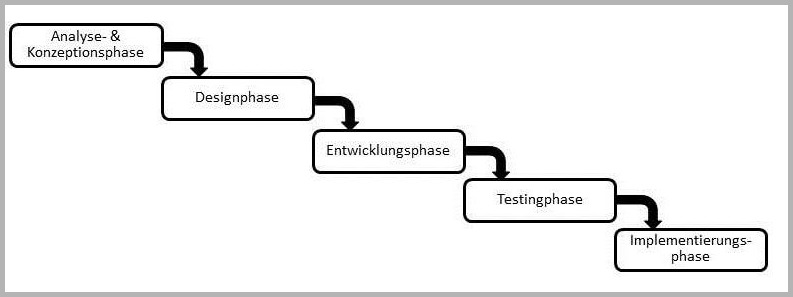
\includegraphics[width=0.6\linewidth]{images/projektmanagement/wasserfallmodell}
	\caption[Wasserfallmodell]{Illustration des Wasserfallmodells \cite{pm-wasserfall-online}}
	\label{fig:wasserfall}
\end{figure}
\subsection{Analyse und Konzeptionsphase}
In dieser Phase wird das Lastenheft und ein Projektstrukturplan erstellt, welche die groben Anforderungen des Projektes verkörpern. Danach wird die Machbarkeit (Grobanforderungen, Kosten, Ertrag, Realisierbarkeit, Umfeldanalyse, Projektorganisation, etc.) des Projektes mittels einer Machbarkeitsstudie analysiert \cite{pm-wasserfall-ionos}. In der Anforderungsdefinition werden alle möglichen Funktionen definiert, die das Software-Projekt beinhalten soll und kann. Diese werden im Pflichtenheft notiert, auch Fachspezifikationen oder Blueprint genannt. Alljene Dinge, die in der \textit{Analysephase} nicht bedacht werden, können im Laufe des Projektes gravierende Folgen auslösen \cite{pm-wasserfall-online}.
\subsection{Designphase}
Die \textit{Designphase} wird streng in Kundenkontakt durchgeführt \cite{pm-wasserfall-online} und ist dafür da, dass ein konkreter Lösungsvorschlag mit den definierten Anforderungen ausgearbeitet wird \cite{pm-wasserfall-ionos}. Es wird eine detaillierte Anleitung für die Erstellung der Software verfasst, die sich vor allem auf Komponenten wie Schnittstellen, Frameworks oder Bibliotheken bezieht. Als Resultat dieser Phase erhält man ein Entwurfsdokument mit Software-Bauplan, bzw. eine technische Spezifikation und Testplänen, die sich auf einzelne Komponenten beziehen.
\subsection{Entwicklungsphase}
In dieser Phase, werden die in der \textit{Designphase} entwickelten Konzepte und Spezifikationen umgesetzt. Der Projektleiter spielt hier eine tragende Rolle, denn er muss sich bei aufkommenden Fragestellungen sowohl um externe, als auch interne Probleme kümmern und in Kontakt mit dem Auftraggeber bleiben \cite{pm-wasserfall-online}. 
\subsection{Testphase}
In der \textit{Testphase} wird das Ergebnis der Entwicklungsphase getestet und auf Fehler geprüft \cite{pm-wasserfall-online}. Sollten diese auftreten werden, sie ausgebessert und einem \textit{Re-Test} zugeführt, bis der Kunde das angefragte und funktionierende Endprodukt hat.
\subsection{Implementierungsphase}
In der \textit{Implementierungsphase} findet der \textit{Rollout} statt, welcher mittels einem \textit{Rolloutplan}, der bereits in der \textit{Designphase} erstellt wurde, durchgeführt wird \cite{pm-wasserfall-online}. Sollte es sich bei dem Projekt um Erweiterungen für eine bestehende Applikation handeln, dann sollte der \textit{Rollout} nicht zu \textit{Peakzeiten} stattfinden.
\section{Agiles Projektmanagement}
\label{chapter:agil-pm}
In agilen Methoden steht vor allem die Funktionalität im Vordergrund und nicht die Dokumentation, wie im traditionellen System \cite{pm-agil-ursula}. Durch die kurzen Iterationen haben Entwickler und Kunden ein besseres Gefühl für das entstehende Produkt und die Kundenwünsche können besser implementiert werden. Alle agile Methoden sind Vorgehensmodelle, die auf einem Wertekanon, Prinzipien und Praktiken beruhen \cite{pm-agil-ursula}. 
\begin{center}
	\textit{\enquote{Agiles Projektmanagement bezeichnet Vorgehensweisen, 
			bei denen das Projektteam über hohe Toleranzen bezüglich Qualität, Umfang, Zeit und Kosten verfügt und eine sehr hohe Mitwirkung des Auftraggebers bei der Erstellung des Werks erforderlich ist. Charakteristisch für agiles Projektmanagement ist die Fokussierung auf das zu liefernde Werk und die Akzeptanz durch die Anwender. Hingegen werden geschäftliche Anforderungen, wie z. B. die Termintreue, Kostentreue oder Erfüllung eines spezifzierten Leistungsumfangs weniger oder nicht berücksichtigt}}  \cite{pm-agil-magazin}.
\end{center}
\subsection{Scrum}
Scrum ist ein empirisches Vorgehen, das in sogenannte \textit{Sprints} (ein zeitlich begrenztes Event) eingeteilt ist \cite{pm-agil-ursula}. Ein \textit{Sprint}, besteht aus dem \textit{Sprint Planning}, in dem der kommende, maximal vier wöchige \textit{Sprint}, geplant und durchgesprochen wird. Genauer gesagt werden Aufgaben von dem \textit{Project Backlog} (der Wunschliste, des Kunden), in den \textit{Sprint Backlog} (die Aufgaben, die das \textit{Development Team} in einem Sprint durchführen wird) verschoben. Jeden Tag im \textit{Sprint} gibt es einen \textit{Daily Scrum}, in dem ein 15 minütiges \textit{Standupmeeting} stattfindet. Dieser Ablauf ist grafisch in \autoref{fig:scrum} dargestellt.
\begin{figure}[H]
	\centering
	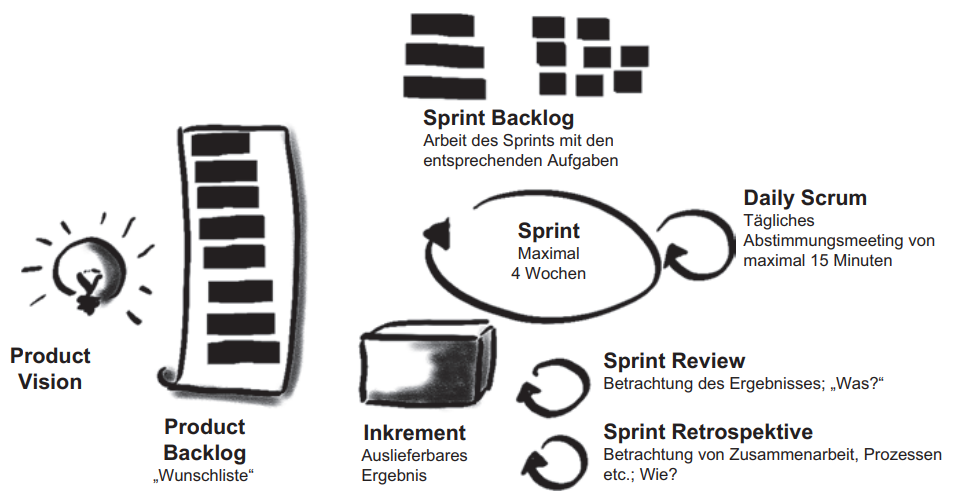
\includegraphics[width=0.6\linewidth]{images/projektmanagement/scrum2}
	\caption[Scrum]{Illustration Scrum \cite{pm-agil-ursula}}
	\label{fig:scrum}
\end{figure}
\subsubsection{Scrum-Rollen}
\paragraph{Product Owner}~\\
Der \textit{Product Owner} trägt die Verantwortung des Produktes. Üblicherweise bringt dieser ein ausgeprägtes Branchenwissen mit sich, das den Erfolg und die Profitabilität des Produktes garantieren soll.
\paragraph{Scrum Master}~\\
Der \textit{Scrum Master} hilft dem \textit{Development Team}, bei der Lösung, spezieller Herausforderungen. Seine Hauptaufgabe ist es, sich sowohl um die Scrum-Werte und Methoden, als auch um die Prozesse zwischen den verschiedenen Rollen zu kümmern.
\paragraph{Development Team}~\\
Das \textit{Development Team} setzt die \textit{Tasks} selbstständig um und erstellt die aus den \textit{Sprints} resultierenden Produktinkremente, die jeweils testbare Einheiten bilden sollten und im Anschluss getestet werden.

\subsection{Kanban}
In \textit{Kanban} gibt es keine bestimmten Rollen, die den Projektmitglieder zugewiesen werden, anders als in Scrum \cite{pm-agil-ursula}. Es gibt ein \textit{Kanban-Board}, welches einen strukturierten Aufbau, von Links nach Rechts beinhaltet. Alle Aufgaben aus dem \textit{Backlog} werden als sogenannte \textit{To do's} ganz Links angezeigt. Des Weiteren gibt es eine Spalte, in der die Aufgaben, die als Nächstes zu behandeln sind gesammelt werden. Dieses Verfahren wird bis zu der Spalte fortgeführt, in welcher die abgeschlossenen \textit{To do's} gesammelt werden. Der Ablauf dieser Spalten ist ähnlich inkrementell, wie bei \textit{Scrum}. Jedoch werden die Arbeitspakete nicht zugeteilt, sondern das \textit{Development Team} zieht sich die \textit{Tickets} selbstständig (auch unter dem Begriff \textit{Pull-Prinzip} bekannt). Siehe \autoref{fig:kanban} zur Veranschaulichung des \textit{Kanban-Boards}. 
\begin{figure}[H]
	\centering
	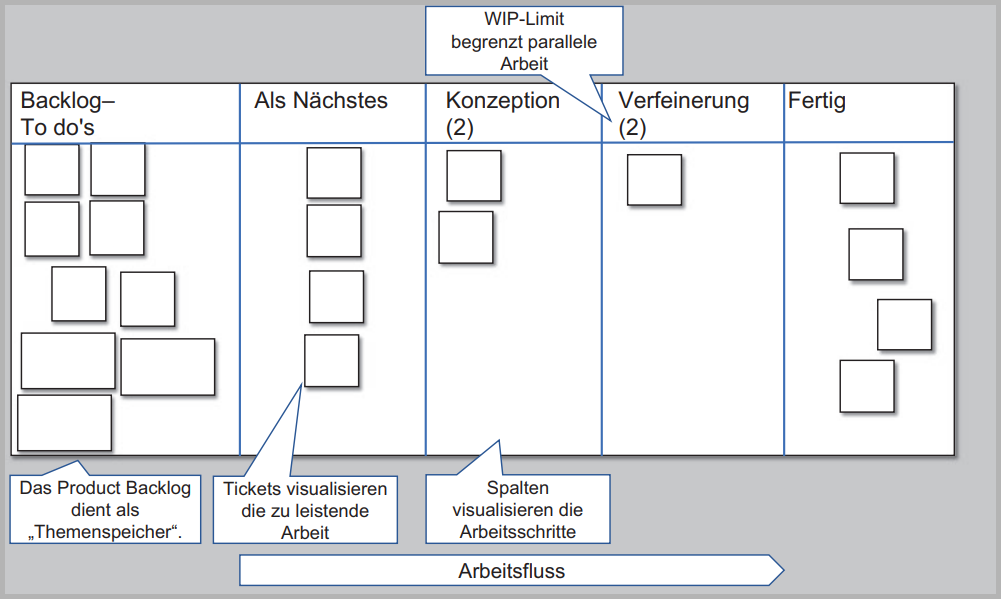
\includegraphics[width=0.6\linewidth]{images/projektmanagement/kanban}
	\caption[Kanban]{Illustration Kanban \cite{pm-agil-ursula}}
	\label{fig:kanban}
\end{figure}
\section{Fazit}
Angesichts des hohen Dokumentationsaufwandes im traditionellen Projektmanagement, hat sich das Team, wegen des Fokus, auf das Endprodukt für eine agile Methode entschieden. Da \textit{Kanban} im Gegensatz zu \textit{Scrum} nicht disruptiv, sondern evolutionär ist und man daher keine neuen Rollen zuweisen muss, hat sich das Projektteam für \textit{Kanban} entschieden, nicht zuletzt ob des geringen Implementierungsaufwandes. Ein weiterer Entscheidungsgrund war, dass das Projektteam parallel zu ihren schulischen Aktivitäten arbeiten muss und gleichmäßige Sprints nicht garantiert möglich sind. Ebenfalls hat die Integration, des \textit{Kanban-Boards} in \textit{GitHub} die Entscheidung für \textit{Kanban} beeinflusst.
\lfoot{Linus Dehner, Michael Beier, Ryan Foster}
%!TEX root=../main.tex
\chapter{Studie}
Unsere Studie beschäftigt sich mit aktuell am Markt befindlichen Technologien und vergleicht diese in einem projektspezifischen Kontext. Auf Basis der Analyse treffen wir schließlich im \hyperref[sec:fazit]{Fazit} eine fundierte Entscheidung über die im Projekt zu verwendenden Technologien, wie Programmiersprachen, \gls{framework}s und Werkzeuge, zur Entwicklung, sowie Auslieferung der Software.
\lfoot{Linus Dehner}
%!TEX root=../../main.tex

\section{Frontend - responsives Webdesign}
\label{chapter:study-frontend}
	\subsection{Einleitung}
	\label{chapter:study-frontend-einleitung}
	In diesem Kapitel werden die Anforderungen des \textit{\Gls{frontend}-Deisgns} geschildert. Da es mehrere Möglichkeiten gibt, das \textit{Frontend} zu realisieren, werden hier drei wesentliche Methoden verglichen. Die erste Variante wäre, ganz klassisch \Gls{html}, \Gls{css} und \Gls{js} zu verwenden. Die zweite Methode, die zum Vergleich herangezogen wird, verwendet statt \Gls{vanilla} CSS die etwas agilere Sprache \Gls{sass}. Die dritte und auch letzte Methode in diesem Vergleich ist, die Arbeit durch die Verwendung eines CSS \Gls{framework}s zu vereinfachen. Anschließend werden die drei verschiedenen Methoden gegenübergestellt und die für unser Projekt \textit{Refundable}, am besten geeignete Variante ausgewählt. Zu guter Letzt wird das Design im Hinblick auf die Zielgruppe der Lehrer analysiert, die sich möglichst gut und schnell auf der Website zurecht finden soll.
	
	\subsection{HTML, CSS, JS}
	\label{chapter:study-frontend-html-css-js}
	Der eigentliche Standard \textit{HTML5} wird in der Praxis meist als Überbegriff für \textit{HTML}, \textit{CSS} und \textit{JS} verwendet \cite{html5-css3-handbuch}. In den folgenden Kapiteln wird erklärt wozu \textit{HTML}, \textit{CSS} und \textit{JS} da sind und welche Funktionalitäten sie bieten.
	
		\subsubsection{HTML}
		\label{chapter:study-frontend-html}
		HTML ist eine \Gls{auszeichnungssprache}, sie steht für \enquote{Hypertext Markup Language} und wurde 1989 von dem britischen Informatiker Tim Burners-Lee veröffentlicht.\\ 
		\begin{center}
			\textit{\enquote{Hypertext bezeichnet die Möglichkeit, Texte mit Hilfe von Hyperlinks, oder kurz Links, miteinander zu verbinden}}\cite{html5-css3-def}.
		\end{center}
		Dies heißt, dass man mittels Hypertexts (Links) auf der Seite beliebig zwischen Sektionen hin und her springen kann.
		Auszeichnungssprachen werden im Fachjargon auch als \textit{Markup Language (ML)} bezeichnet \cite{auszeichnungssprachen}. \textit{Markup Languages} werden in zwei verschiedene Gruppen aufgeteilt, zum einen \textit{Procedural Markup Languages (PML)}, das sind jene Auszeichnungssprachen, die für die Verarbeitung von Daten optimiert sind. Zum anderen \textit{Descriptive Markup Languages (DML)}, diese sind für die logische Strukturierung von Daten da.\\Bekannte Beispiele hierfür sind:
		\begin{itemize}
		\item PML
		\subitem PDF
		\subitem TeX
		\item DML
		\subitem HTML
		\subitem SVG
		\end{itemize}
	\captionof{listing}{PML/DML Beispiele}
	\label{list:dmlbsp}~\\
		\textit{HTML} wird hauptsächlich verwendet, um Texte, Grafiken und Hyperlinks (Links) darzustellen \cite{html5-css3-handbuch, html5-css3-def}. Die Bearbeitung von \textit{HTML-Dokumenten} ist relativ einfach und unkompliziert, da es eine rein textbasierte Sprache ist und mit jedem Texteditor bearbeitet werden kann.\\
		Allerdings ist \textit{HTML} nicht mit einer Programmiersprache zu verwechseln, da nur \Gls{tag}s und keine Befehle oder Anweisungen verwendet werden. Solche Tags können wie folgt aussehen:
		\begin{code}{html}
			<tagname>Tag Inhalt</tagname>
			<einzeltag attribut="123">
		\end{code}
	\captionof{listing}{HTML Tags}
	\label{list:htmltags} ~\\
		Das grundlegende Gerüst von HTML besteht aus einer Deklaration von HTML, einem \textit{html-}, \textit{head-} und \textit{body-Tag}. In den \textit{html-Tag} kommt ein \textit{title-Tag}, in diesem wird der Titel der Website angegeben und ein \textit{meta-tag}, in diesem werden Meta-Informationen angegeben. In den \textit{Body-Tag} kommen wiederum Tags, die den Inhalt der Seite darstellt. 
		\begin{code}{html}
			<!DOCTYPE html>
			<html lang="de">
				<head>
					<meta charset="UTF-8">
					<meta name="viewport" content="width=device-width, initial-scale=1.0">
					<title>Kurzes BSP</title>
				</head>
				<body>
					<h1>Überschrift</h1>
					<button>Drück mich!</button>
				</body>
			</html>
		\end{code}
	\captionof{listing}{Kurzes HTML Beispiel}
	\label{list:htmlbsp} ~\\
		Wenn man die Datei nun im Browser öffnet, sieht dies wie folgt aus:
		\begin{figure}[H]
			\centering
			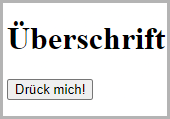
\includegraphics[width=0.2\linewidth]{images/ldehner_study/html1}
			\caption[HTML Beispielseite]{Beispiel einer HTML Seite mit einer Überschrift und einem Button}
			\label{fig:htmlbsp}
		\end{figure}
		~\\
		Da \textit{HTML} nur für die Grundstruktur einer Website gedacht ist, also zum Beschreiben der Struktur und des Inhalts, ist das Design noch nicht sonderlich ansprechend. Um dies zu verändern, wird CSS benötigt.
		
		\subsubsection{CSS}
		\label{chapter:study-frontend-css}
		\textit{Cascading Stylesheets}, oder kurz \textit{CSS}, ist für den \textit{Style}, also für das Aussehen der Website verantwortlich. Da \textit{HTML} anfangs nur im Printbereich verbreitet wurde, war es nicht notwendig, die Seiten zu gestalten \cite{html5-css3-def, html5-css3-handbuch}. Das Internet bekam aber einen immer stärker werdenden Einfluss und daher auch eine höhere Bekanntheit. Deswegen wurde \textit{HTML} mit der Formatierungssprache \textit{CSS} ergänzt.\\
		Mittels CSS sind unter anderem folgende Dinge möglich:
		\begin{itemize}
			\item Hintergrund ändern
			\item Schrift ändern
			\item Die Website automatisch an die Bildschirmgröße anpassen
			\item Den Formfaktor von Elementen verändern
			\subitem Größe
			\subitem Rand
			\subitem Farbe
			\subitem Form
			\subitem Schatten
			\subitem Hover-Effekt
		\end{itemize}
	\captionof{listing}{Beispiele Verwendung von CSS}
	\label{list:bspcss}~\\
		Man kann \textit{CSS} auf verschiedene Arten in \textit{HTML} benützen. Als Beispiel werden wir eine Überschrift in die Mitte der Website setzen, die Schriftgröße auf \textit{40pt} stellen und die Schriftart auf \enquote{sans-serif} ändern.\\
		Die Umsetzung kann auf mehrere Arten erfolgen. Beispielsweise fügt man einem Element ein \textit{Style-Attribut} hinzu und ändert direkt im Element das Aussehen. Hierbei ist darauf zu achten, dass nur das Element, in dem man diese Änderungen vornimmt, verändert wird:
		\begin{code}{html}
			<h1 style="text-align: center; font-size: 40pt; font-family: sans-serif;">Ich bin eine tolle Überschrift</h1>
		\end{code}
	\captionof{listing}{Beispiele Verwendung von Inline-CSS}
	\label{list:bspinlinecss}~\\
		Man kann auch im \enquote{head} einen \textit{style-Bereich} eröffnen und dort das Aussehen verändern. Dabei ist darauf zu achten, dass man den Style von allen Elementen mit dem Tag, den man ausgewählt hat, verändert. Um dies zu verhindern kann man Elementen auch eine \textit{ID} (für einzelne Elemente verwendbar), oder eine \textit{CLASS} (für mehrere Elemente verwendbar) hinzufügen, sowie diese im CSS-Code auswählen und verändern:
		\begin{code}{html}
				<head>
					<style>
					//Für das ganze Element
					h1 {
						text-align: center; 
						font-size: 40pt; 
						font-family: sans-serif;
					}
				
					//Für IDs
					#ueberschrift1 {
						text-align: center; 
						font-size: 40pt; 
						font-family: sans-serif;
					}
					
					//Für Klassen
					.ueberschriftenGruppe {
						text-align: center; 
						font-size: 40pt; 
						font-family: sans-serif;
					}
					</style>
				</head>
		\end{code}
	\captionof{listing}{Beispiel CSS}
	\label{list:cssbsp} ~\\
		Ebenfalls kann man ein \textit{CSS-File}, welches den Inhalt des obigen \textit{style-Tags} hat, im \textit{head} als externes File einbinden:
		\begin{code}{html}
			<head>
				<link rel="stylesheet" href="file.css" type="text/css">
			</head>
		\end{code}
	\captionof{listing}{CSS Verlinkung}
	\label{list:csslink} ~\\
		Wie man erkennen kann, ist dem ganzen kein Ende gesetzt und mit viel Aufwand kann man alles Denkbare verändern. Um den Aufwand jedoch gering zu halten, sind \textit{SASS} und \textit{CSS-Frameworks} da, welche in \autoref{chapter:study-frontend-sass} und \autoref{chapter:study-frontend-frameworks} erklärt werden.
		\subsubsection{Java Script}
		\label{chapter:study-frontend-js}
		\textit{JavaScript} wird verwendet, um Elementen Funktionen zu geben. Zum Beispiel, dass wenn man auf einen Button drückt, ein Fenster aufpoppt, ein neues Element hinzugefügt wird, oder ein Element im Nachhinein verändert wird. Da \textit{JavaScript} eine Skriptsprache ist, kann man auch eigene Funktionen schreiben und Variablen verwenden. Für das Designen braucht man JS nur, wenn man mit \textit{CSS} oder \textit{SASS} arbeitet. Wird ein \textit{Framework} verwendet, hat dieses meist ein \textit{JavaScript-Framework} inkludiert und man muss kein \textit{JavaScript} mehr verwenden.
	\subsection{SASS}
	\label{chapter:study-frontend-sass}
	\textit{Syntactically Awesome Style Sheets} oder kurz \textit{SASS} ist eine Erweiterung von \textit{CSS} \cite{jump-start-sass}. Es fügt \textit{CSS} ein paar Funktionalitäten von Java Script hinzu. \textit{SASS} wird aber nicht wie \textit{CSS} direkt in das \textit{HTML-File} eingebunden und kann auch nicht direkt in ein Element geschrieben werden. Das \textit{.sass} File muss erst kompiliert werden. Anschließend wird ein \textit{.css} File generiert, welches man im \textit{HTML-Code} einbinden kann. Man kann unter anderem Funktionen erstellen, um Elemente zu verändern. Zusätzlich kann man Variablen kreieren und so zum Beispiel eine Primärfarbe festlegen, wodurch man sich nicht immer den \textit{HEX-Code} von einer bestimmten Farbe merken muss. Ebenfalls kann man durch die Variablen die Farbe von mehreren Elementen auf einmal ändern. Dadurch kann man zum Beispiel Light- und Darktheme in die Website einbauen.

%	\begin{code}{sass}
	%	$standard-width: 200px
	%	$standard-color: #03f0fc
	%	
	%	.button {
	%		background-color: $standard-color;
	%		width: $standard-width;
	%	}
	%
	%	.button big{
	%		background-color: $standard-color;
	%		width: multiply($standard-width, 2);
	%	}
	%
	%	@function multiply($a, $b) {
	%		@return ($a * $b);
	%	}
%	\end{code}
	
	
	\subsection{Frameworks}
	\label{chapter:study-frontend-frameworks}
	Frameworks für HTML, CSS und JS beinhalten vorgestaltete Komponenten, welche mittels Klassen, einem HTML Element hinzugefügt werden. Da Frameworks das Arbeiten an einer Website wesentlich einfacher machen und wir dieses Hilfsmittel auch benutzen werden, müssen folgende Fragen beantwortet werden, um das optimale Framework für dieses Projekt auszuwählen:
	\begin{itemize}
		\item \textbf{Welche CSS-Frameworks unterstützen explizit die User-Experience und Usability?}
		\item \textbf{Welche Vor- und Nachteile bringen diese Frameworks mit sich?}
	\end{itemize}
\captionof{listing}{Fragestellungen - Frameworks}
\label{list:fragenframeworks} ~\\
	Zum Vergleich werden vier sehr verbreitete und geschätzte Frameworks herangezogen:
		\subsubsection{Bootstrap}
		\label{chapter:study-frontend-frameworks-bootstrap}
		Bootstrap ist ein Framework, welches am bekanntesten ist und am meisten verwendet wird \cite{introduction-bootstrap, learning-bootstrap}. Das von Twitter entwickelte Framework hat in der aktuellen Version 4.5 viele verschiedene Komponenten, die optimal für erfahrene Entwickler, aber auch für Anfänger geeignet sind. In der Dokumentation von Bootstrap gibt es einige Templates und sehr viel gut dokumentierten Beispiel Code\cite{introduction-bootstrap}. Bootstrap kann über einen Paketmanager, ein CDN, oder als heruntergeladene Datei zur HTML Datei hinzugefügt werden \cite{bootstrap-docu}. Durch diesen großen Verwendungsgrad gibt es viele Erweiterungen und zahlreiche Plattformen auf denen man sich informieren kann, falls man Probleme bei der Entwicklung der Website hat \cite{learning-bootstrap}. Bootstrap bietet, mit seinem überschaubaren Grid-System, eine gute Umsetzung für die Responsivität der Seite, damit sie auf allen möglichen Endgeräten perfekt aussieht.
		\paragraph{Pro / Contra}
		\subparagraph{Pro}
		\begin{itemize}
			\item HTML/CSS/JS Framework
			\item Umfangreich
			\item Mittels SASS veränderbar
			\item Zahlreiche Erweiterungen
			\item Viele Erkundungsmöglichkeiten
			\item Viele Einbindungsmöglichkeiten
			\item Arbeitet gut mit VueJS zusammen
			\item Responsiv
		\end{itemize}
	\captionof{listing}{Bootstrap Pro}
	\label{list:bootstrappro}
		\subparagraph{Contra}
		\begin{itemize}
			\item Viele Websites sehen gleich aus
			\item Komplexer zu erlernen
			\item Kein schönes Standarddesign
		\end{itemize}
	\captionof{listing}{Bootstrap Contra}
	\label{list:bootstrapcontra}
	
		\subsubsection{Materialize}
		\label{chapter:study-frontend-frameworks-materialize}
		Materialize ist wie Bootstrap ein intuitives HTML, CSS und JS Framework \cite{materialize-intro}. Es ist Bootstrap sogar sehr ähnlich, aber simpler aufgebaut. Dadurch hat es auch nicht so viele verschiedene Komponenten und nicht so viel Beispiel Code wie Bootstrap. Materialize legt vor allem Wert auf das Design, welches von Google's Material Design abstammt. Ein weiterer großer Punkt ist Usability und User Experience, welche unter anderem Hand in Hand mit dem Design gehen. Um die User Experience möglichst hoch zu halten, arbeitet Materialize viel mit Animationen. Materialize kann ebenfalls über ein \Gls{cdn}, Paketmanager oder als Datei in das Projekt eingebunden werden. Falls man das Design verändern will, stellt Materialize ebenfalls noch eine SASS Version zur Verfügung \cite{WebDocMaterialize}.
		\paragraph{Pro / Contra}
		\subparagraph{Pro}
		\begin{itemize}
			\item HTML/CSS/JS Framework
			\item Mittels SASS veränderbar
			\item Ansehnliches Standard-Design 
			\item Viele Animationen
			\item Viele Einbindungsmöglichkeiten
			\item Einfach zu verstehen
			\item Responsiv
		\end{itemize}
	\captionof{listing}{Materialize Pro}
	\label{list:materializepro}
		\subparagraph{Contra}
		\begin{itemize}
			\item Einige Probleme mit VueJS
			\item Weniger Erkundungsmöglichkeiten
			\item Beispielcode ist oft unvollständig
		\end{itemize}
	\captionof{listing}{Materialize Contra}
	\label{list:materializecontra}
	
		\subsubsection{ZURB Foundation}
		\label{chapter:study-frontend-frameworks-foundation}
		Foundation wird wie Bootstrap und Materialize, als intuitives Web-Framework bezeichnet \cite{foundation-intro}. Das von Zurb entwickelte Framework beinhaltet viele verschiedenen Komponenten, die für mobile Endgeräte optimiert sind. Mit dem Framework können Webseiten schnell und effizient gestaltet werden. Darum ist es auch in zwei verschiedene Kategorien geteilt, in das Framework für das Web und in das Framework, welches explizit für html-Mails gedacht ist. In der \enquote{Complete-Version} sind alle Komponenten enthalten. In der \enquote{Essential-Version} sind nur die essentiellen Komponenten, wie zum Beispiel Buttons, enthalten. Man kann sich seine ZURB-Datei auch mit allen Komponenten, die man benötigt, selbst konfigurieren. Auch eine SASS Version ist verfügbar, falls man nur das Aussehen der Komponenten verändern möchte. Natürlich ist auch eine CDN Einbindung möglich, die für die schnellste Ladegeschwindigkeit optimiert ist.
		\paragraph{Pro / Contra}
		\subparagraph{Pro}
		\begin{itemize}
			\item HTML/CSS/JS Framework
			\item Mittels SASS veränderbar
			\item Auf Bedürfnisse anpassbar
			\item Ansehnliches Standard-Design 
			\item Viele Einbindungsmöglichkeiten
			\item Einfach zu verstehen
			\item Responsiv
		\end{itemize}
	\captionof{listing}{ZURB Foundation Pro}
	\label{list:zurbpro}
		\subparagraph{Contra}
		\begin{itemize}
			\item Keine persönliche Erfahrung
			\item Relativ junges Framework
			\item Nicht so viele Erkundungsmöglichkeiten
			\item Kein ansprechendes Standarddesign
		\end{itemize}
	\captionof{listing}{ZURB Foundation Contra}
	\label{list:zurbcontra}

	\subsection{Vergleich}
	\label{chapter:study-frontend-vergleich}
	Der Vergleich der Frameworks setzt sich aus dem Umfang, den Erweiterungen, dem Aussehen, der Leichtigkeit im Bezug auf das Erlernen des Frameworks, dem Umfang der Dokumentation, der Kompatibilität mit VueJS und unserer Erfahrung, mit dem jeweiligen Framework zusammen.\\
	Die Punkte (0-9) setzen sich immer in der Relation mit den anderen Frameworks zusammen, wobei 9 die Beste, also maximale Punktzahl ist. Die Basis 0 ist in diesem Vergleich mit den Funktionen und Aufwand von Vanilla CSS gleichzusetzen. Alle dafür benötigten Informationen wurden von der jeweiligen Dokumentationsseite bezogen.
	~\\
	\captionof{table}[Vergleich HTML Frameworks]{Vergleich zwischen Bootstrap, Materialize und Foundation}\label{tbl:comparison}
	\begin{center}
		\begin{table}
			\centering
		\begin{tabular}{rccc}
			\hline
			\multicolumn{1}{|r|}{{\underline{\textbf{Kriterien}}}} & \multicolumn{1}{c|}{{\underline{\textbf{Bootstrap}}}} & \multicolumn{1}{c|}{{ \underline{\textbf{Materialize}}}} & \multicolumn{1}{c|}{{\underline{\textbf{Foundation}}}} \\ \hline
			\multicolumn{1}{|r|}{\textbf{Umfang}}          & \multicolumn{1}{c|}{9}                        & \multicolumn{1}{c|}{9}                          & \multicolumn{1}{c|}{7}                         \\ \hline
			\multicolumn{1}{|r|}{\textbf{Erweiterungen}}   & \multicolumn{1}{c|}{9}                        & \multicolumn{1}{c|}{3}                          & \multicolumn{1}{c|}{7}                         \\ \hline
			\multicolumn{1}{|r|}{\textbf{Aussehen}}        & \multicolumn{1}{c|}{6}                        & \multicolumn{1}{c|}{9}                          & \multicolumn{1}{c|}{5}                         \\ \hline
			\multicolumn{1}{|r|}{\textbf{Leichtigkeit}}    & \multicolumn{1}{c|}{6}                        & \multicolumn{1}{c|}{9}                          & \multicolumn{1}{c|}{8}                         \\ \hline
			\multicolumn{1}{|r|}{\textbf{Dokumentation}}   & \multicolumn{1}{c|}{9}                        & \multicolumn{1}{c|}{6}                          & \multicolumn{1}{c|}{9}                         \\ \hline
			\multicolumn{1}{|r|}{\textbf{Kompatibilität}}  & \multicolumn{1}{c|}{9}                        & \multicolumn{1}{c|}{5}                          & \multicolumn{1}{c|}{7}                         \\ \hline
			\multicolumn{1}{|r|}{\textbf{Erfahrung}}       & \multicolumn{1}{c|}{5}                        & \multicolumn{1}{c|}{9}                          & \multicolumn{1}{c|}{0}                         \\ \hline
			\textbf{Gesamt}                                & 53                                            & 50                                              & 43                                            
		\end{tabular}
	\end{table}
	\end{center}
\subsubsection{Umfang}
\label{chapter:study-frontend-vergleich-umfang}
Die Punktevergabe des Umfangs setzt sich zusammen aus der Anzahl, der Komponenten und Hilfsklassen. Bootstrap und Materialize haben in etwa die selbe Anzahl (53 \& 55) und bekommen daher die Maximalpunktzahl \cite{bootstrap-docu,WebDocMaterialize,foundation-webdocu}. Foundation hat hingegen deutlich weniger Komponenten (41), als die anderen zwei Frameworks und hat daher nur 7 Punkte bekommen.
\subsubsection{Erweiterungen}
\label{chapter:study-frontend-vergleich-erweiterungen}
Bootstrap hat durch das langjährige Bestehen und durch die große Reichweite unzähliger Erweiterungen, die Schwächen, wie zum Beispiel das Standarddesign wieder auszumerzen. Deswegen hat Bootstrap hier auch die volle Punkteanzahl bekommen \cite{introduction-bootstrap}. Materialize hat nur kostenpflichtige, offizielle Plugins, deswegen hat dieses Framework nur 3 Punkte bekommen. Foundation hingegen, hat wiederum eine ausreichende Auswahl an Plugins, die sogar in der Dokumentation verlinkt sind \cite{foundation-webdocu}. 
\subsubsection{Aussehen}
\label{chapter:study-frontend-vergleich-aussehen}
Bei dem Aussehen des Standard-Designs gewinnt klar und deutlich Materialize, da es die ansprechendste Darstellung mit einem schönen Design bietet \cite{WebDocMaterialize}. Bootstrap und Foundation legen mehr Wert auf die Funktionalität des Frameworks und weniger auf das Aussehen \cite{bootstrap-docu, foundation-webdocu}. Dies merkt man daran, dass die Elemente optisch nur minimal von den HTML-Standardelementen abweichen. Materialize hat hingegen ein komplett neues und modernes Design aufgezogen.
\subsubsection{Leichtigkeit}
\label{chapter:study-frontend-vergleich-leichtigkeit}
Aus eigener Erfahrung können wir sagen, dass Materialize wirklich einfach zu erlernen ist \cite{WebDocMaterialize}. Bei einem groben Einlernen in Foundation hat das Team festgestellt, dass es dem Aufbau von Materialize sehr ähnelt. Bootstrap hingegen sah auf den ersten Blick sehr kompliziert aus und war am Anfang sehr schwer zu verstehen. Nach ein paar Stunden Einlernen war schon ein sehr guter Workflow vorhanden.
\subsubsection{Dokumentation}
\label{chapter:study-frontend-vergleich-doku}
Auf den ersten Blick erscheint die Dokumentation von Materialize als sehr gut, jedoch ist der Beispielcode zu einzelnen Komponenten in manchen Fällen unvollständig und man muss sich mit mühsamer Recherche nach Lösungen erkunden \cite{WebDocMaterialize}. Bootstrap und Foundation sind sehr gut dokumentiert, haben viele Code-Beispiele und sind in manchen Fällen sogar mit \Gls{codepen} Beispielen bestückt \cite{bootstrap-docu, foundation-webdocu}.

\subsubsection{Kompatibilität}
\label{chapter:study-frontend-vergleich-kompatibilität}
Wie in \autoref{chapter:study-datenschnittstelle} erklärt wird, werden wir als JS Framework VueJS verwenden. Kompatibel sind alle Frameworks, jedoch ist Bootstrap für die Zusammenarbeit mit Vue optimiert \cite{bootstrap-docu}. Da das Projektteam in einem früheren Projekt bereits Materialize mit Vue benutzt hat, ist bekannt, dass in Verbindung der beiden Frameworks Probleme auftreten können. Foundation ist nicht speziell dafür optimiert mit Vue zusammenzuarbeiten. Die Funktionalität ist trotzdem vorhanden. Jedoch wurde Foundation bis jetzt von keinem Mitglied der Projektes in Verbindung mit Vue verwendet.

\subsubsection{Erfahrung}
\label{chapter:study-frontend-vergleich-erfahrung}
Das Frontend-Team hat bis jetzt hauptsächlich Erfahrung mit Materialize gemacht. Bootstrap wurde in der Schule kurz angeschnitten, aber im privaten Umfeld etwas vertieft. Mit Foundation hingegen wurde noch keine Erfahrung gesammelt.

\subsection{Fazit}
\label{chapter:study-frontend-vergleich-fazit}
Nach dem Vergleich, der in dieser Arbeit durchgeführt wurde, ist es leicht, die optimale Auswahl der Umsetzung für Refundable zu treffen. Eine Entwicklung ohne ein Framework kommt auf Basis der Analyse nicht zu Stande, da der Aufwand für die Umsetzung, wesentlich höher wäre. Wir haben uns schließlich für Bootstrap entschieden, da es im Vergleich eindeutig am besten abschneidet und auch am Besten mit VueJS harmoniert.


\lfoot{Michael Beier}
%!TEX root=../../main.tex

\section{Backend - REST-Schnittstelle und Infrastruktur}
\label{chap:backendsota}
	\subsection{Einleitung}
	Das Backend besteht aus mehreren Komponenten. Einerseits soll eine gewisse System-Infrastruktur aufgebaut werden, um das \gls{webinterface} und die REST-Schnittstelle bereitzustellen. Andererseits muss die Anwendung selbst entwickelt werden. Diese besteht aus mehreren Teilen. Darunter fällt die REST-Schnittstelle, inklusive der implementierten Endpoints, Schnittstellen zu diversen Diensten, wie dem TGM-LDAP Server, zur Datenbank und zu WebUntis, aber auch die allgemeine Funktionalität der Anwendung, unter anderem das Erstellen von PDF-Dateien. Für die Verbindung zu den Schnittstellen sowie zur Implementierung der geforderten Funktionalität werden diverse  \gls{tpp} genutzt werden. Die folgende Grafik gibt einen Überblick hinter der Infrastruktur und den verwendeten Diensten:
	\begin{figure}[H]
		\centering
		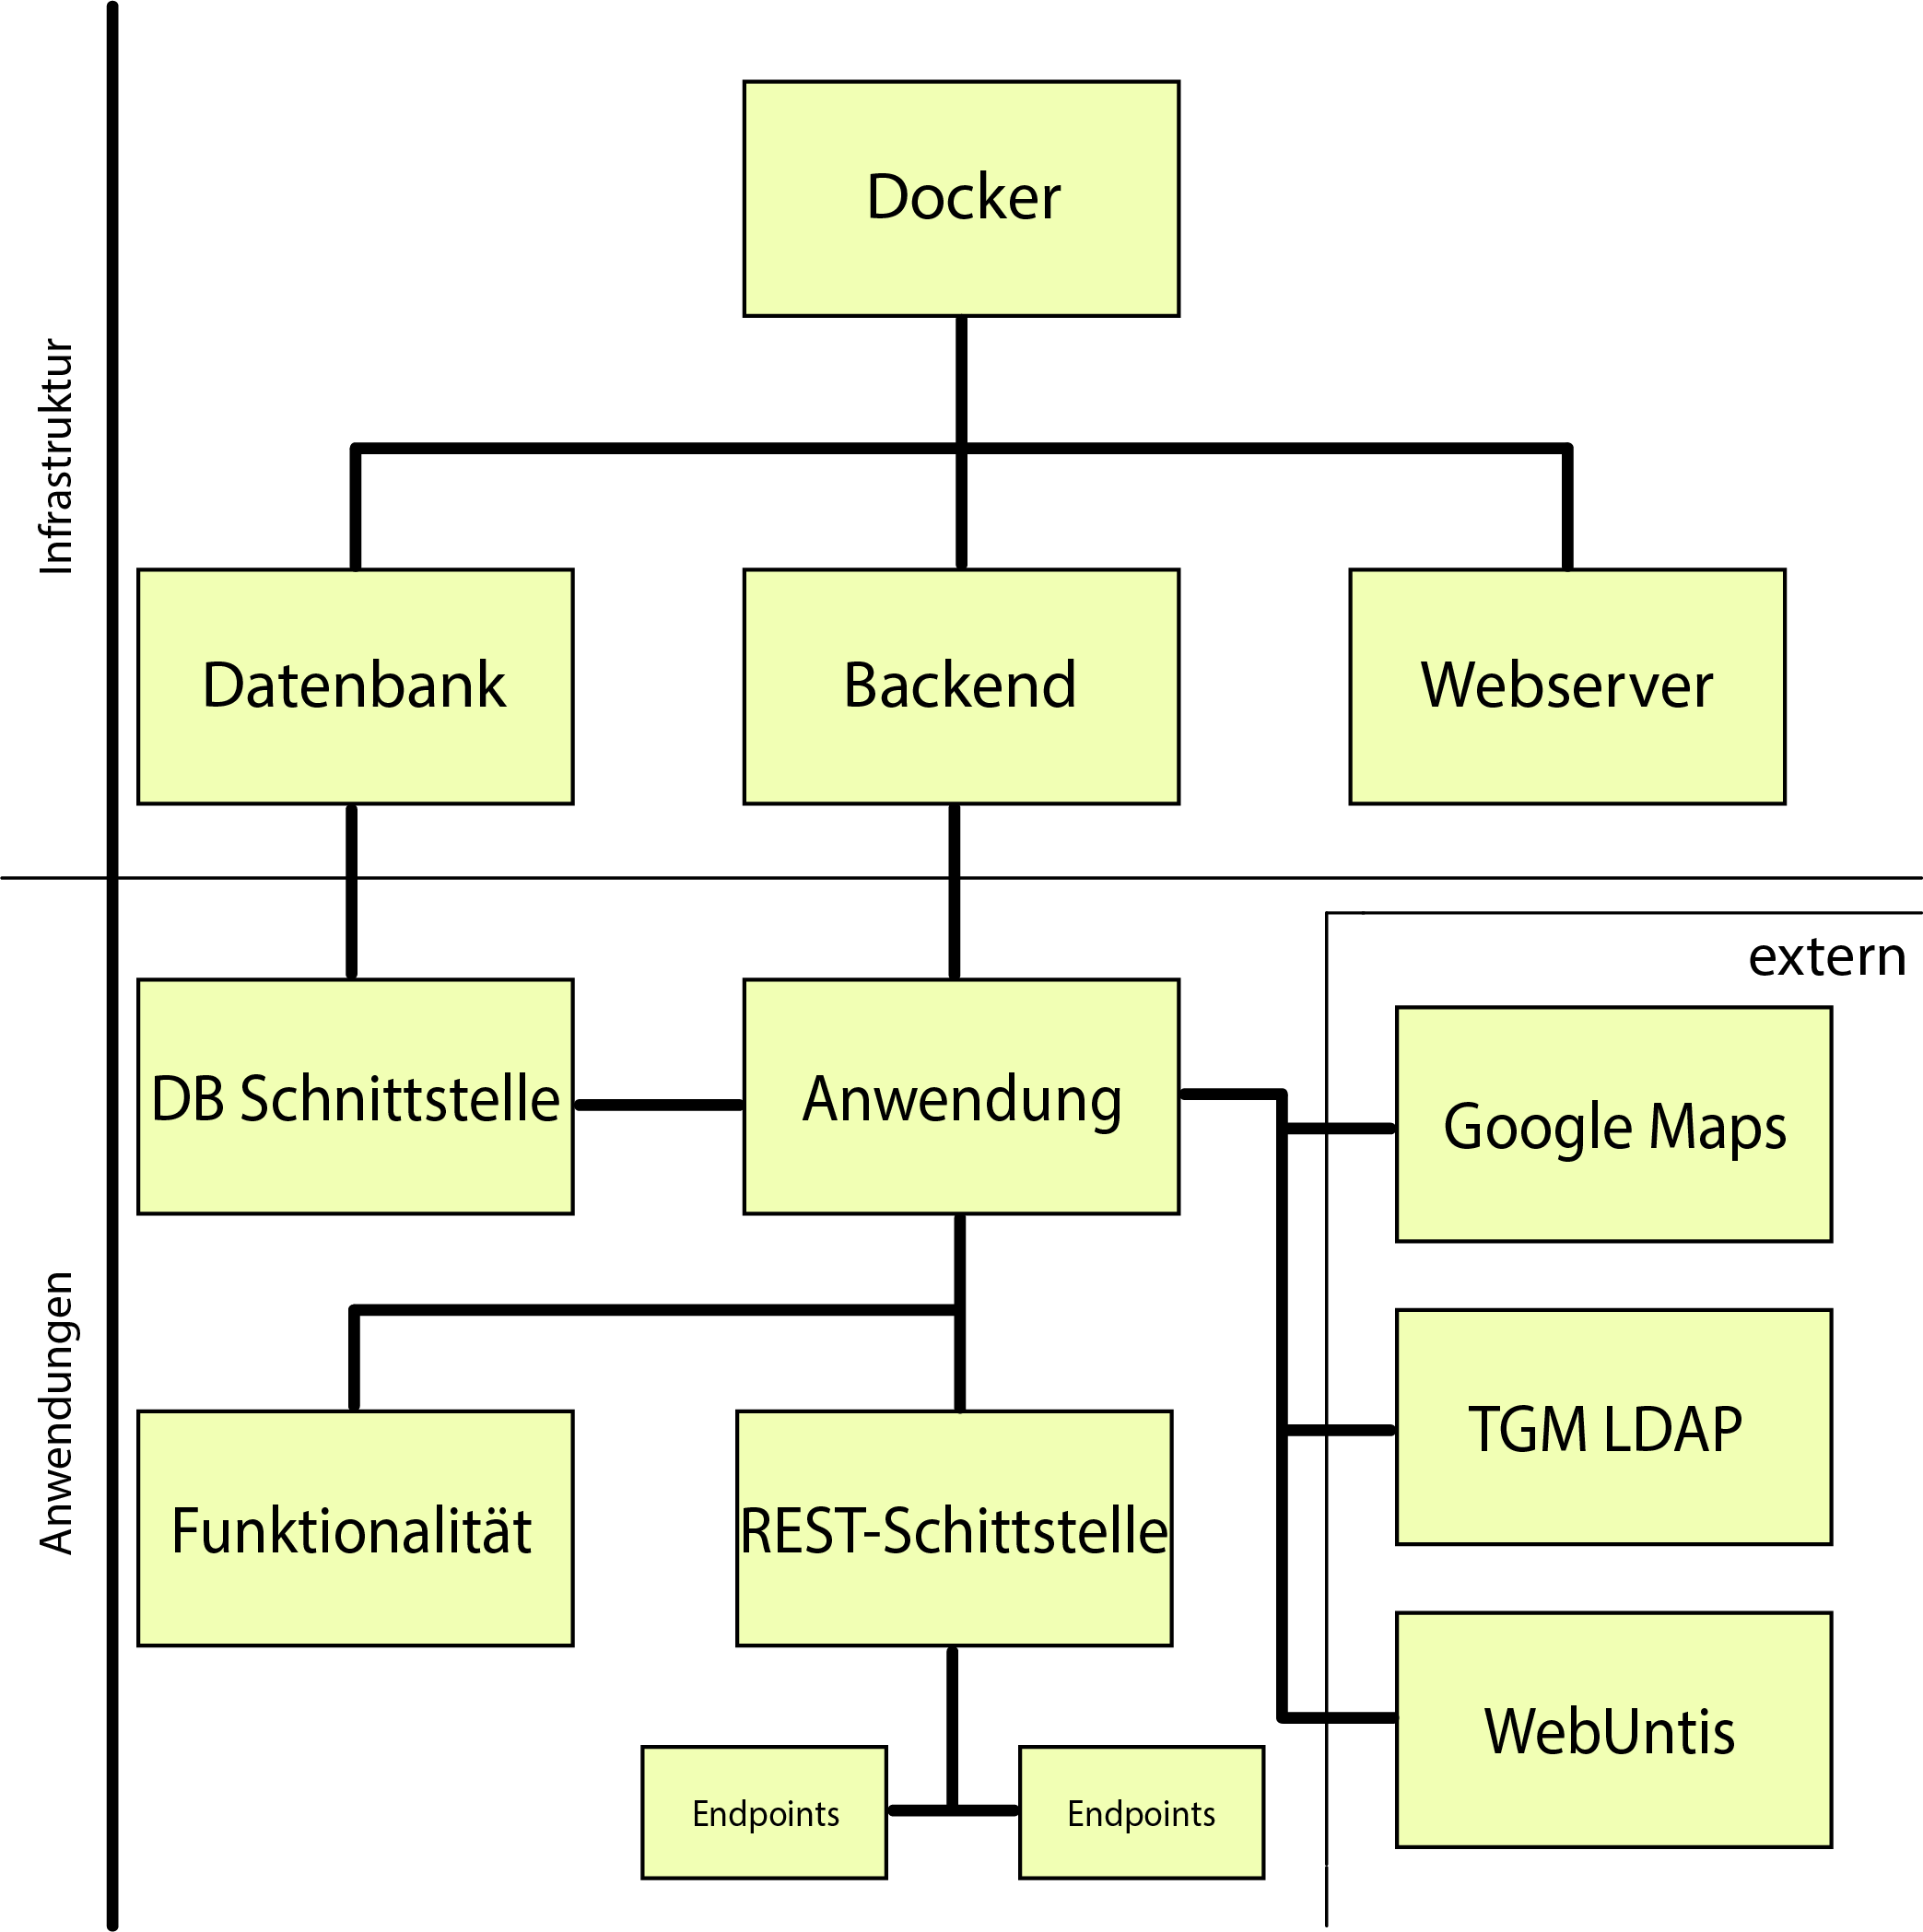
\includegraphics[width=0.8\linewidth]{images/uebersicht}
		\caption[Übersicht über die Komponenten]{Übersicht über die verschiedenen Komponenten der Infrastruktur und der Anwendung}
		\label{fig:uebersicht}
	\end{figure}
	
	\newpage
	In den folgenden Kapiteln werden die aktuell verfügbaren Technologien, welche für die Umsetzung im Backendbereich in Frage kommen, beschrieben und gegebenenfalls - sofern mehrere sinnvolle Kandidaten vorhanden sind - auch verglichen. Auf einen detaillierten Vergleich jeglicher verwendbaren Third Party Packages, welche dazu genutzt werden könnten, um die Funktionalität im Backend zu implementieren, wird auf Grund der extrem hohen Anzahl im Sinne der Übersichtlichkeit verzichtet. Unter die benutzten Packages, fallen jedenfalls Module wie maroto (zum Erstellen von PDF-Dateien \cite{maroto}), excelize (zum Erstellen von Excel-Dateien \cite{excelize}) und jwt-go (zum Erstellen von \Gls{jwt} \cite{jwt-go}) 
	\subsection{Docker}
	Um die Infrastruktur des Projektes einfach aufbauen zu können, wird \Gls{docker} genutzt. Da es sich hier um eine komplex strukturierte Infrastruktur handelt, wird zusätzlich das Werkzeug \Gls{dcompose} genutzt. Mit Docker Compose kann eine Infrastruktur aufgebaut werden, die der \hyperref[fig:uebersicht]{Abbildung 5.2} entspricht. Für diese sind folgende Container vorgesehen, die in den nächsten Kapiteln noch im Detail beschrieben werden.
		\subsubsection{Datenbank}
		\label{sec:db}
		Um die Daten, die durch Refundable erhoben und generiert werden, zu speichern, wird eine \gls{db} benötigt. Auf Grund der Daten, welche sich durch unterschiedliche Datenstrukturen auszeichnen, ist der Einsatz einer \gls{relDb} nicht sinnvoll. Stattdessen empfiehlt sich die Verwendung einer \gls{nosqlDb}.
		Standardmäßig wird zwischen 4 verschiedenen Typen von NoSQL Datenbanken unterschieden, welche jeweils nur in ihrem eigenen Use Cases sinnvoll anwendbar sind \cite{nosqltypes}:
		\begin{itemize}
			\item Key-Value Datenbank
			\item spaltenorientierte Datenbank
			\item graphenorientierte Datenbank
			\item dokumentenorientierte Datenbank
		\end{itemize}
		\captionof{listing}{NoSQL Datenbank-Typen}
		\label{code:nosqltypes}~\\	
		Bei Key-Value Datenbanken wird einem Schlüssel ein Wert hinterlegt. Dieser Wert ist dann jederzeit über den Schlüssel in der Datenbank abrufbar. Für unseren Use Case ist dieses System nicht sinnvoll anzuwenden, da die von uns benutzten Daten hierfür zu komplex im Aufbau sind.~\\
		Bei spaltenorientierten Datenbanken werden Daten vorrangig über ihre Spalten (statt wie bei relationalen \gls{db}s in Zeilen) analysiert. Dies ermöglicht die einfache Umsetzung statistischer Methoden auf Basis der Spalten. Da jedoch wieder eine Tabelle als Grundstruktur vorliegt, ist dieser Typ von Datenbank nicht sinnvoll anwendbar für Refundable.~\\
		Bei graphenorientierten Daten wird die Beziehung zwischen einzelnen Elementen hervorgehoben. Daten werden hier in Knoten gespeichert, welche zu anderen verbunden werden können. Die primären Elemente sind hierbei die Beziehungen, anstatt der Daten selbst. Da die Daten von Refundable nicht über starke Beziehungen charakterisiert sind, ist auch dieser Datenbank-Typ nicht sinnvoll zu benutzen.~\\		
		Zuletzt bei dokumentenorientierten Datenbanken unterliegt jeder Datensatz in einem eigenen Dokument, welches in \Gls{json}, \Gls{yaml}, \Gls{xml} oder ähnlichen Datenformaten gespeichert wird. Dadurch ist auch eine jeweils von einander unabhängige Datenstruktur möglich. Auf Grund der Flexibilität bei Datenstrukturen ist eine dokumentenorientierte Datenbank eindeutig sinnvoll zu verwenden.~\\
		Als \gls{dbms} kommt bei dieser Auswahl einige Software in Frage. Die am meisten verbreitete Software hier ist MongoDB und CouchDB \cite{mongo}. Wo MongoDB auf strenge \gls{konsistenz} setzt, setzt CouchDB auf hohe \gls{verfugbarkeit}. Da in unserem Projekt Konsistenz wichtiger ist als Verfügbarkeit wird MongoDB in einem Container als Datenbankmanagementsystem verwendet.
		
		\subsubsection{Backend-Container}
		
		Ebenfalls wird ein Container, also eine Umgebung, in dem das Backend laufen kann, erstellt. Dieser wird direkt zu den anderen Containern hinzugefügt, damit dieser über ein Docker-Netzwerk mit den anderen Containern kommunizieren kann.~\\
		Um diesen Container zu realisieren wird als Basis ein golang-Image genutzt \cite{golang}. Dieses stellt eine sehr sparsame Linux-Instanz dar, welche mit einer golang-Umgebung ausgestattet ist. Um diesen Container noch entsprechend anzupassen, wird ein entsprechendes Docker-Image über ein Dockerfile gebaut.
		
		\subsubsection{Webserver}
		
		Als Webserver wird ein Apache2 Server genutzt \cite{apache}. Der Service stellt hierbei das Webinterface (Frontend) im Internet zur Verfügung. Dieser Container ruft automatisch das Frontend auf und kopiert es in seine Umgebung. Ebenfalls muss der Container Zugriff auf Zertifikaten bekommen, um einen sicheren Zugriff über \gls{https} gewährleisten zu können.
				
	\subsection{Deployment}
	
	Das Deployment soll automatisch geschehen. Um dies einfach zu ermöglichen, werden die oben zuvor beschriebenen Docker-Container, GitHub und ein Skript, welches die Schritte ausführt, genutzt. Das Skript ist hier der Hauptbaustein, welcher den Vorgang startet und steuert. Zusätzlich zum Installationsvorgang, soll das Skript auch die weitere Steuerung der Software, also starten, stoppen, updaten, cleanen und deinstallieren, beinhalten.~\\
	Das Skript liegt in einem eigenem Install-\Gls{repo}, in welchem sonst keine weiteren Dateien liegen. Dadurch kann es einfach geklont und direkt installiert werden; die restlichen Installations-Schritte werden automatisch erledigt.~\\
	Da das Deployment auf einer Linux-Maschine ermöglicht werden soll, wird \Gls{bash} als Standard-Skriptsprache benutzt. Zur Verteilung des Scripts wird, wie erwähnt, \Gls{git} mit dem Online Repository-Hosting Service \Gls{github} verwendet.
	\subsection{REST-Schnittstelle}
	Bei einer REST-Schnittstelle handelt es sich um einen bestimmten Aufbau einer Softwareschnittstelle bei verteilten Systemen \cite{Patni2017}. Das hierbei angewendete Prinzip nennt sich \enquote{Representational State Transfer} (kurz REST). Es zeichnet sich durch folgende Eigenschaften aus:
	\begin{itemize}
		\item \textbf{Client-Server}, wobei es um eine strikte Trennung zwischen dem Client (dem REST-Client) und dem Server (der REST-Schnittstelle, als Webservice) geht
		\item \textbf{Stateless}, wobei es um die Zustandslosigkeit des Servers geht. Das heißt, dass der Server sich keinerlei Zustände der Clients merkt.
		\item \textbf{Caching}: Der Server speichert die Responses zwischen. Dadurch kann die Latenzzeit minimiert werden, da Daten öfters zurückgegeben werden, anstatt sie jedes Mal erneut berechnen zu müssen.
		\item \textbf{Einheitliche Schnittstelle} bedeutet, dass die Schnittstelle ein einheitliches Datenformat verwendet, um via HTTP über CRUD-Methoden (Create, Read, Update, Delete) zu kommunizieren.
		\item \textbf{Layer-System} bedeutet, dass die Schnittstelle, als Webservice so designed wird, dass auch weitere Schichten, wie Gateways und Proxies, transparent dazwischen aufgebaut werden können.
		\item \textbf{Code-on-demand} (optional): Hierbei besteht die Möglichkeit ausführbaren Code an die Clients zu schicken, sodass diese den dann ausführen können.
	\end{itemize}
	\captionof{listing}{Prinzipien des Representation State Transfer}
	\label{code:rest}
		\subsubsection{Java und Spring}
		Java ist eine der bekanntesten Programmiersprachen. Sie zeichnet sich durch Plattform-Unabhängigkeit aus \cite{jdkDocs}. Um dies zu erreichen, wird Bytecode von einem eigenem Programm, der Java Virtual Machine, interpretiert. Java arbeitet objektorientiert und ist statisch typisiert. Dies bedeutet, dass bereits vor dem Ausführen die Datentypen definiert sind. Java unterstützt auch Multithreading. Um einfach eine REST-Schnittstelle in Java bauen zu können, wird Spring Boot genutzt \cite{springDocs}. Die Verwendung von Spring ermöglicht Webapps, Tasks oder Microservices einfacher umzusetzen. Prinzipiell arbeitet Spring asynchron und flexibel, sodass es einfach zu skalieren ist. 
		
		\subsubsection{Python und Flask}
		Um mit Python eine REST-Schnittstelle zu realisieren muss auf das Package (Framework) Python Flask zurückgegriffen werden \cite{flaskDocs}. Flask wird hierbei dazu genutzt, um den Webservice zu bauen. Python und Java unterscheiden sich prinzipiell sehr. Python ist im Gegensatz zu Java dynamisch typisiert, dies bedeutet, dass eine Variablendeklaration nicht notwendig ist und der Datentyp einer Variable erst zur Laufzeit klar ist \cite{pythonDocs}. Anders als Java setzt Python auf Third-Party Packages, welche sehr einfach importiert werden können. Durch die große Community Pythons ist ein Großteil der Tools, die man benötigt, meist schon vorprogrammiert und kann einfach importiert werden. Zusätzlich ist der Syntax (speziell was Zeichensetzung anbelangt) einfacher zu verstehen, als jener von Java.
		
		\subsubsection{Golang}
		\label{chapter:golanganalyse}
		Golang (kurz Go) ist eine von Google entwickelte und publizierte Programmiersprache \cite{goDocs}. Sie wurde aus der Unzufriedenheit über Java, C++ und Python heraus entwickelt, welche am häufigsten bei Google eingesetzt wurden. All diese Programmiersprachen haben Nachteile in Googles Business Case, deswegen wurde Go speziell für skalierbare Netzwerkdienste und Cloud Computing entwickelt. Aus diesem Grund besitzt Go auch eine native Möglichkeit für den einfachen Aufbau von REST-Schnittstellen. Da bei der Entwicklung von Go speziell aus den Fehlern in Performance und Sprachdesign aus anderen Sprachen gelernt wurde, verbindet Go die Vorteile der anderen Sprachen. Darunter fallen die starke und statische Typisierung, Objektorientierung, Pointer und eine verbesserte Compiler-Effizienz.
		\newpage
		\subsubsection{Vergleich}
		Diese drei Sprachen werden nun in den Aspekten der Performance, dem Sprachdesign, der Komplexität des Aufbaus einer REST-Schnittstelle, das Vorhandensein von Frameworks, die Erfahrung des Teams und eine vorhandene ausführliche Dokumentation analysiert und verglichen. Hierbei wird auf einer Punkteskala von 0 - 9 bewertet.
		\captionof{table}{Vergleich zwischen Java, Python und Golang}\label{tbl:comparisonlang}
		\begin{table}
			\begin{tabular}{|l|r|r|r|r|r|r|r|}
				\hline
				\multicolumn{1}{|c|}{\textbf{Kriterien}} & \multicolumn{1}{c|}{\textbf{Gewichtung}} & \multicolumn{2}{c|}{\textbf{Java und Spring}} & \multicolumn{2}{c|}{\textbf{Python und Flask}} & \multicolumn{2}{c|}{\textbf{Golang}} \\ \cline{3-8} 
				& \multicolumn{1}{l|}{} & \multicolumn{1}{c|}{Punkte} & \multicolumn{1}{c|}{Wertung} & \multicolumn{1}{c|}{Punkte} & \multicolumn{1}{c|}{Wertung} & \multicolumn{1}{c|}{Punkte} & \multicolumn{1}{c|}{Wertung} \\ \hline
				Performance & 15\% & 6 & 0,9 & 3 & 0,45 & 9 & 1,35 \\ \hline
				Sprachdesign & 25\% & 6 & 1,5 & 4 & 1 & 8 & 2 \\ \hline
				\begin{tabular}[c]{@{}l@{}}Aufbau einer \\ REST-Schnittstelle\end{tabular} & 5\% & 7 & 0,35 & 8 & 0,40 & 9 & 0,45 \\ \hline
				\begin{tabular}[c]{@{}l@{}}Vorhandensein von\\ Frameworks\end{tabular} & 15\% & 7 & 1,05 & 9 & 1,35 & 9 & 1,35 \\ \hline
				\begin{tabular}[c]{@{}l@{}}Erfahrung des \\ Teams\end{tabular} & 20\% & 4 & 0,8 & 3 & 0,6 & 6 & 1,2 \\ \hline
				Dokumentation & 20\% & 8 & 1,6 & 7 & 1,4 & 9 & 1,8 \\ \hline
				\textbf{Summe} & 100\% & \multicolumn{1}{l|}{} & \multicolumn{1}{c|}{\textbf{6,2}} & \multicolumn{1}{c|}{\textbf{}} & \multicolumn{1}{c|}{\textbf{5,2}} & \multicolumn{1}{c|}{\textbf{}} & \multicolumn{1}{c|}{\textbf{8,15}} \\ \hline
			\end{tabular}
		\end{table}
		~\\
		Daraus und aus der durchgeführten Recherche, lässt sich schließen, dass Golang sich speziell bei den Punkten Performance und Sprachdesign durchsetzen kann. Ansonsten schneiden die verschiedenen Sprachen inklusive der teilweise benötigten Frameworks großteils ähnlich hoch ab. Zusammenfassend eignet sich die Verwendung von Golang am Besten als Programmiersprache für unser Projekt, da sie im numerischen Vergleich mit der höchsten Punktezahl abschnitt, aber auch durch die speziellen Hintergründe ihrer Entwicklung genau zu den Voraussetzungen passt.
	\subsection{Kommunikation und Datenformate}
	Wie bereits erwähnt, zeichnen sich REST-Schnittstellen unter anderem dadurch aus, dass sie ein einheitliches Datenformat voraussetzen. Aus diesem Grund stellen sich die Fragen: \\~\\
	Welche Datenformate eignen sich für einen konsistenten und performanten Datenaustausch zwischen Datenbank, REST-Schnittstelle und Client? \\~\\
	Welche Vor- und Nachteile bringen diese im Hinblick auf Performance, Softwarewartung und -evolution?\\~\\
	Um diese Fragen zu beantworten werden in den nächsten Kapiteln entsprechende Datenformate vorgestellt, beschrieben und analysiert.
	
	\newpage
		\label{sec:json}
		\subsubsection{JSON}
		\Gls{json} (JavaScript Object Notation) ist ein Textformat, welches für die Serialisierung von Daten genutzt werden kann \cite{rfc4627}. 
		Es umfasst 6 Datentypen, davon 4 Primitive und 2 Strukturen:
		\begin{itemize}
			\item \Gls{string}s
			\item Zahlen
			\item \Gls{bool}s
			\item \Gls{null}
			\item \Gls{array}s
			\item \Gls{object}e
		\end{itemize}
		\captionof{listing}{JSON - Datentypen}
		\label{code:jsontypes}~\\	
		Wie so eine Serialisierung aussieht, wird in folgendem Beispiel ersichtlich: 
		
		\begin{code}{json}
		{
			"classes": [
				{
					"name": "1AHIT",
					"lastYear": false,
					"students": 35,
					"class-rep": "Michaela Musterfrau"
				},
				{
					"name": "5BHIT",
					"lastYear": true,
					"students": 25,
					"class-rep": "Maximilian Frühmann"
				}
			],
			"date": "2021-09-01"
		}
		\end{code}
		\captionof{listing}{JSON Beispiel}
		\label{code:json}~\\
		Das in \hyperref[code:json]{Auflistung 5.8} stehende Beispiel stellt ein Objekt mit zwei Feldern dar. Das erste Feld ist ein \enquote{classes}-Array, welches verschiedene Schulklassen beinhaltet. Diese Schulklassen haben jeweils einen String als Namen, einen Boolean als Feld, das angibt, ob es sich um eine Abschlussklasse handelt, die Anzahl der Schüler als Zahl und den Namen des Klassensprechers. Nachdem die Definition des Arrays abgeschlossen ist, wird noch ein weiteres Feld im obersten Objekt angegeben, welches das aktuelle Datum als String beinhaltet.
		\\~\\
		Der JSON-Standard umfasst genaue Regeln, wie mit den Datentypen, speziell mit Strings und Zahlen, umzugehen ist \cite{rfc4627}.
		Über einen JSON-Generator kann ein JSON-Text auf Basis eines Dateninputs generiert werden. Wenn die Daten aus dem JSON-Textformat wieder extrahiert werden sollen, spricht man vom \enquote{parsen} von Daten.\\
		Jede moderne Programmiersprache hat einen eigenen JSON-Parser implementiert oder es ist möglich einen über ein \Gls{tpp} zu laden.
		\subsubsection{XML}
		\Gls{xml} (Extensible Markup Language) ist ein strukturiertes textbasiertes Datenformat \cite{xmlStandard}. Es handelt sich hierbei um eine Markup-Language. Als Syntax von XML werden Tags verwendet. Ein <Tag> ist ein Anfangs-Tag und ein </Tag> ein End-Tag. Ebenfalls können Attribute in einem Anfangs-Tag definiert werden (<Tag attribut=\dq wert\dq ). XML-Dateien brauchen im Gegensatz zu JSON-Texten ein Wurzelelement.
		\begin{code}{xml}
		<school>
			<classes>
				<class lastYear="false" students="35" class-rep="null">1AHIT</class>
				<class lastYear="true" students="25" class-rep="null">5BHIT</class>
			</classes>
			<date>2021-09-01</date>
		</school>
		\end{code}
		\captionof{listing}{XML Beispiel}
		\label{code:xml}~\\
		Das Beispiel definiert ein Wurzelelement für die Datenstruktur namens \enquote{school}. Dieses hat ein Kindelement \enquote{classes}. In diesem sind einzelne \enquote{class}-Tags mit den nötigen Attributen und dem Namen der Klasse innerhalb der Tags. Dies wird als Alternative für die in XML nicht vorhandenen Arrays genutzt. Zuletzt wird wieder ein untergeordnetes \enquote{date}-Element mit dem aktuellem Datum als Inhalt hinzugefügt.\\~\\
		Das XML-Dateiformat kann entweder gültig oder wohlgeformt sein \cite{xmlStandard}. Dies beschreibt die Einhaltung des Syntax und der Regeln des XML Standards.\\
		Des Weiteren besteht die Möglichkeit die Struktur von XML-Dateien anhand der XML-Schema-Sprache oder durch die Document Type Definition zu beschreiben. XML Dateien brauchen aus diesen Gründen unbedingt einen Parser für die Umwandlung.
		
		\newpage
		
		\subsubsection{CSV}
		CSV (Comma-Separated Values) ist ein Textformat, mit welchem man Tabellen textbasiert darstellen kann \cite{rfc4180}. Hierbei werden Spalten durch \dq , \dq  ~(Beistriche) getrennt und Zeilen durch einen Zeilenumbruch (CRLF; LF). Die erste Zeile repräsentiert die Namen der Spalten. Eine Beschreibung einer Tabelle mit CSV sieht wie folgt aus:
		\begin{code}{python}
			Class,lastYear,students,class-rep
			1AHIT,false,35,null
			5BHIT,true,25,null
		\end{code}
		\captionof{listing}{CSV Beispiel}
		\label{code:csv}~\\
		Im Beispiel werden die beiden Klassen als zwei Datensätze in einer Tabelle aufgelistet. Auf Grund der Struktur von CSV ist es nur möglich den Array-Teil des Objektes darzustellen. Ansonsten ist der CSV-Standard recht simpel gehalten. Der letzte Punkt auf den der Standard hierbei eingeht ist, dass "-Zeichen um die Daten gesetzt werden können \cite{rfc4180}. Sollten, diese nicht geschlossen werden kann es jedoch zu unvorhersehbaren Verhalten kommen.
		\subsubsection{Vergleich}
		Ein Vergleich zwischen den Datenformaten JSON, XML und CSV ist auf dem ersten Blick nicht zielführend. Wie aus den einzelnen Beschreibungen der Technologien oben entnommen werden kann, handelt es sich beim CSV-Format um Tabellen. Bereits bei der \hyperref[sec:db]{Wahl der dokumentenorientierten Datenbank MongoDB} war der Hintergedanke relationale Datenbanken und ihrer Speicherstruktur, Tabellen, weitestmöglich zu vermeiden. 
		
		Wenn man sich nun auch das CSV Format und speziell das \hyperref[code:csv]{Beispiel} anschaut, merkt man, dass die Umwandlung des ursprünglichen Objektes nur indirekt möglich war und als Auflistung der Klassen endete. Das Resultat ist, dass Objekte zu CSV-Tabellen mit vielen Spalten und einer Zeile werden und Arrays zu Tabellen mit wenigen Spalten und vielen Zeilen. Eine Darstellung beider Datentypen in einer Tabelle ist nicht möglich. Dies disqualifiziert CSV für den Einsatz als Datenformat im Projekt.
		
		Vergleicht man nun JSON und XML so scheinen diese erst ähnlich. Jedoch besteht bei XML keine Möglichkeit Arrays zu definieren. Des Weiteren wird XML nicht nur als Datenformat zur Kommunikation genutzt, sondern hat noch weitere Nutzen als Markup Language. Demnach ist XML sehr überladen, speziell deswegen weil es einen eigenen speziellen XML-Parser braucht.
		
		Auch JSON braucht einen sogenannten Parser, jedoch handelt es sich hierbei nur um das Einlesen des JSON-Textes und dem Generieren des Objekts. Eine Validierung wie in XML bleibt aus. Zuletzt ist JSON nicht nur schneller, sondern auch effizienter was den Verbrauch an CPU-Leistung und an Arbeitsspeicher angeht \cite{Nurseitov}.
		
		Aus diesen Gründen wird JSON als Datenformat zur Kommunikation zwischen den einzelnen Komponenten Refundables genutzt werden.
\lfoot{Ryan Foster}
%!TEX root=../../main.tex

\section{Frontend - Webapplikation als REST-Client}
\subsection{Einleitung}
Das \Gls{backend} muss mit dem \Gls{frontend} verbunden werden. Es gibt unterschiedliche Möglichkeiten dies zu realisieren. Beim Realisieren muss darauf geachtet werden, dass eine Struktur vorhanden ist. Es werden zwei verschiedene \Gls{designpattern} betrachtet und verglichen. Umgesetzt wird dann ein Entwurfsmuster mithilfe von \Gls{js}. Hier kann ein \Gls{js}-\Gls{framework} zum Einsatz kommen. Dazu werden hier verschiedene JavaScript-Frameworks miteinander verglichen. Für die Verarbeitung der Daten ist es wichtig, Datenformate festzulegen. Die Aufbereitung der Elemente für das Frontend mit den Daten des Backends wird ebenfalls untersucht.
\\\\
Die Fragestellung der Studie ist erstens, welche Unterschiede es bei der Datenrepräsentation und -manipulation zwischen den Entwurfsmustern Model-View-ViewModel (\Gls{mvvm}) und Model-View-Controller (\Gls{mvc}) gibt und zweitens, mit welchen Werkzeugen bzw. JavaScript-Frameworks die jeweiligen Methoden zugriffsperformant umgesetzt werden können.
\subsection{Entwurfsmuster}
Dieser Teil des Projektes wird in Verwendung eines Entwurfsmusters umgesetzt. Zwei \Gls{mv*} Entwurfsmuster werden hierbei in Betrachtung gezogen: zum einen MVVM und zum anderen MVC. Es kommen diese zwei Entwurfsmuster in Frage, da MVC ein sehr bekanntes Entwurfsmuster ist und MVVM eine neuere und spezifischere Variante von MVC ist \cite{mvvm_vue}.
\subsubsection{MVC}
\Gls{mvc} ist ein Entwurfsmuster, mit dem eine Software in die drei Teile (Model, View und Controller) geteilt wird \cite{mvc}. Das Model beinhaltet alle Daten der Software und auch alle Funktionen, die mit den Daten interagieren oder mit ihnen rechnen. Die View ist der Teil der Software, den Benutzer sehen und mit dem sie interagieren. Dieser Teil der Software beinhaltet keine wichtigen Daten oder Funktionen, welche Daten bearbeiten. Die View hört nur auf Benutzereingaben und zeigt die bereitgestellten Daten an. Der Controller ist der Teil der Software, der Model und View verbindet. Im Controller wird auf die Benutzereingaben reagiert und es werden die gewünschten Funktionen aus dem Model aufgerufen.
\begin{figure}[H]
	\centering
	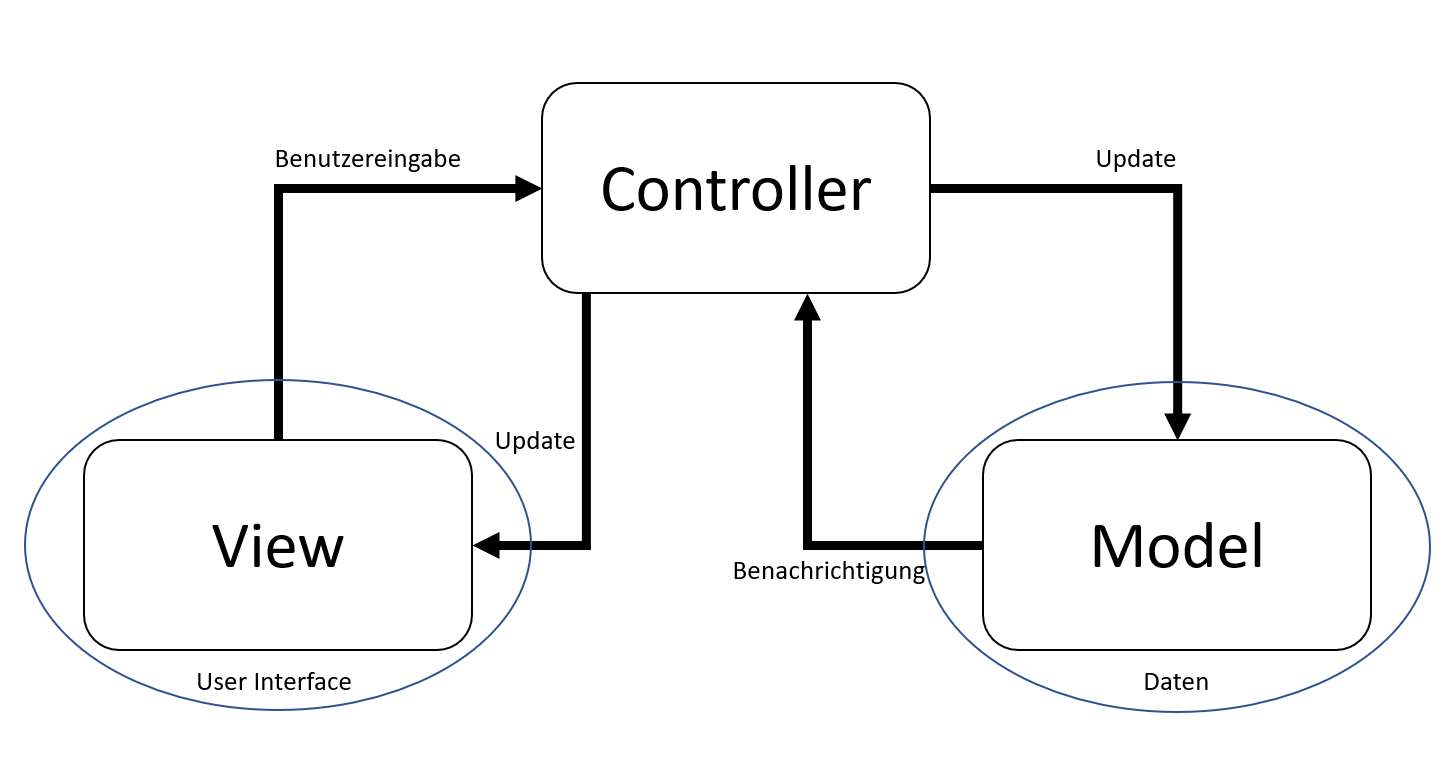
\includegraphics[width=0.8\linewidth]{images/mvc}
	\caption[Übersicht des MVC-Patterns]{Übersicht über die Komponenten des MVC-Patterns und ihre Zusammenhänge}
	\label{fig:mvc}
\end{figure}
\subsubsection{MVVM}
\Gls{mvvm} oder auch \Gls{mvvc} ist ein \Gls{designpattern} mit dem eine Software in drei Teile geteilt wird \cite{mvvm_vue}. Jedoch wird bei MVVM die Software in Model, View und ViewModel aufgeteilt. 
Das Model beinhaltet, wie im konventionellen \Gls{mvc}-Pattern, alle wichtigen Daten und Funktionen. 
Die View ist, wie beim MVC-Pattern, der Teil der Software, mit dem der Benutzer interagiert. 
Das ViewModel ist ein Bindeglied zwischen Model und View \cite{mvvm_vue}. Dabei stellt das ViewModel der View Funktionen zur Verfügung. Diese können auch Daten verändern bzw. mit Daten rechnen. Das Model kann über das ViewModel auch mit der View direkt interagieren. 
MVVM sieht nicht vor, dass ein Controller verwendet wird. Diese Funktion übernimmt zu einem gewissen Teil das ViewModel bzw. auch die View und das Model.
\begin{figure}[H]
	\centering
	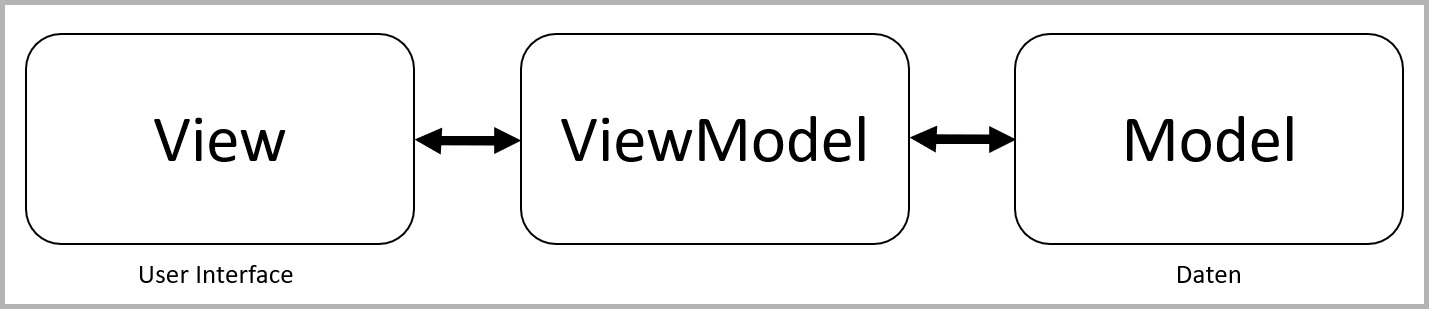
\includegraphics[width=0.8\linewidth]{images/mvvm}
	\caption[Übersicht des MVVM-Patterns]{Übersicht über die Komponenten des MVVM-Patterns und ihre Zusammenhänge}
	\label{fig:mvvm}
\end{figure}
\subsubsection{Vergleich}
Diese zwei \Gls{designpattern} sind zwar sehr ähnlich, jedoch gibt es wichtige Unterschiede zwischen ihnen.\\\\
\Gls{mvc} ist ein Entwurfsmuster, welches auf einem niedrigen Level überall im Einsatz ist - z.B. bei Tastatureingaben \cite{mvc}. Dieses Entwurfsmuster ist zwar schon lange verfügbar, jedoch kann es bei Webapplikationen zu Problemen führen.\\
Bei der Entwicklung einer Webapplikation ist es nicht einfach, das Model von dem Controller zu trennen.\\
\Gls{mvvm} auf der anderen Seite zielt explizit auf HTML5 ab \cite{mvvm_vue}. Somit ist es bei webbasierten Applikationen zu bevorzugen.
\newpage
\subsection{Umsetzungsmöglichkeiten}
Dieser Teil des Projekts wird mittels \Gls{js} umgesetzt. Hierbei kommen unterschiedliche \Gls{js}-\Gls{framework} in Frage. Hier werden die verbreitetsten JavaScript-Frameworks vorgestellt und dann verglichen. \Gls{angular} wird nicht in Betrachtung gezogen, da dies ein \Gls{framework} für professionelle Projekte ist und demnach nicht für vergleichsweise kleine Projekte verwendbar ist, wegen dem Aufwand das Framework zu erlernen \cite{angular_ex}.
\subsubsection{VueJS}
\gls{vue} ist ein progressives JavaScript-Framework. Dies bedeutet, dass VueJS in bereits bestehende Webseiten bzw. in webbasierte Software implementiert werden kann.\\
VueJS kann aber auch von Anfang an verwendet werden, wobei man hier mit den Bibliotheken von VueJS skalieren kann \cite{vuedoc}. VueJS kann Teile einer Webseite in Komponenten aufteilen, um diese mehrmals zu verwenden, falls dies notwendig ist. Jeder dieser Komponenten hat sein eigenes \Gls{html}-, \Gls{css}- und \Gls{js} File, die gebraucht werden, um diese Komponente zu rendern.\\
Um einzelnen Elementen VueJS-Funktionalität zu geben, kann auf diese Elemente folgender Code angewendet werden \cite{vuedoc}:
\begin{code}{html}
	<!DOCTYPE html>
	<html lang="de">
		<head>
			<meta charset="UTF-8">
			<meta name="viewport" content="width=device-width, initial-scale=1.0">
			<title>Kurzes VueJS-Beispiel</title>
		</head>
		<body>
			<h1>Überschrift</h1>
			<div id="app">
				<!-- Der Text, welcher weiter unten Definiert wird, wird hier eingefügt -->
				<!-- Ändert sich die Variable, dann ändert sich auch der Text auf der Webseite -->
				<p> {{ text }} </p>
			</div>
			<script src="https://unpkg.com/vue"></script>
			<script>
				const app = new Vue({
					el: '#app',
					data: {
						text: 'Hier steht Text!'
					}
				})
			</script>
		</body>
	</html>
\end{code}
\captionof{listing}[VueJS Beispiel]{Beispiel für VueJS Webseite}~\\
\subsubsection{React}
\Gls{react} ist eine \Gls{js}-Bibliothek, mit der man Benutzeroberflächen entwickeln kann \cite{reactdoc}. React hat, wie \Gls{vue}, Komponenten. Dies bedeutet, dass man einzelne Elemente mehrfach verwenden kann, falls man dies benötigt.\\
React wurde von Facebook entwickelt und wurde 2013 als \Gls{opensource}-Lösung veröffentlicht.\\
Folgender Code beschreibt eine Beispiel-React-Webseite \cite{reactdoc}:
\begin{code}{html}
	<!DOCTYPE html>
	<html lang="de">
		<head>
			<meta charset="UTF-8">
			<meta name="viewport" content="width=device-width, initial-scale=1.0">
			<title>Kurzes React-Beispiel</title>
		</head>
		<body>
			<h1>Überschrift</h1>
			<div id="likebuttoncontainer"></div>
			
			<!-- Load React. -->
			<!-- Note: when deploying, replace "development.js" with "production.min.js". -->
			<script src="https://unpkg.com/react@17/umd/react.development.js" crossorigin></script>
			<script src="https://unpkg.com/react-dom@17/umd/react-dom.development.js" crossorigin></script>
			<!-- Load our React component. -->
			<script src="likebutton.js"></script>
		</body>
	</html>
\end{code}
\captionof{listing}[React-Webseite Beispiel]{Beispiel für React Webseite}~\\
\newpage
In der letzten Zeile des body-Tags, wird auf \textit{likebutton.js} referenziert. Dies ist eine Komponente und muss noch erstellt werden \cite{reactdoc}:
\begin{code}{js}
	'use strict';
	
	const e = React.createElement;
	
	class LikeButton extends React.Component {
		constructor(props) {
			super(props);
			this.state = { liked: false };
		}
		
		render() {
			if (this.state.liked) {
				return 'You liked this.';
			}
			
			return e(
			'button',
			{ onClick: () => this.setState({ liked: true }) },
			'Like'
			);
		}
	}
	
	const domContainer = document.querySelector('#likebuttoncontainer');
	ReactDOM.render(e(LikeButton), domContainer);
\end{code}
\captionof{listing}[React-Komponente Beispiel]{Beispiel für eine React-Komponente}
\newpage
\subsubsection{Ohne Framework}
Die Schnittstelle zwischen \Gls{backend} und \Gls{frontend} kann auch ohne ein \Gls{framework} umgesetzt werden. Dies ist bei kleinen und leichten Applikationen von Vorteil, da keine umständlichen \Gls{js}-\Gls{framework}s aufgesetzt und richtig implementiert werden müssen. Ohne Framework implementiert man eine \Gls{js}-Datei in eine Webseite, um die gewünschte Funktionalität einzufügen. Mit folgendem Code kann eine Implementierung einer JavaScript-Datei umgesetzt werden:
\begin{code}{html}
	<!DOCTYPE html>
	<html lang="de">
		<head>
			<meta charset="UTF-8">
			<meta name="viewport" content="width=device-width, initial-scale=1.0">
			<title>Kurzes Plain-Beispiel</title>
		</head>
		<body>
			<div id="inhalt">
				<h1>Überschrift</h1>
			</div>
			<!-- Die Implementierung der JavaScript-Datei -->
			<script src="javascript.js"></script>
		</body>
	</html>
\end{code}
\captionof{listing}[Ohne Framework Beispiel]{Beispiel für Webseite ohne Framework}~\\
Es kann auch direkt in ein \Gls{html}-File \Gls{js} in ein \textit{<script></script>} geschrieben werden.
\newpage
\subsubsection{Vergleich}

Verglichen werden diese unterschiedlichen Umsetzungsmöglichkeiten an Design, Entwicklungszeit, Performanz und \Gls{loc}.\\
Die Webseite, die für den Vergleich umgesetzt werden soll, wird mit den unterschiedlichen Umsetzungsmöglichkeiten umgesetzt.\\
\begin{figure}[H]
	\centering
	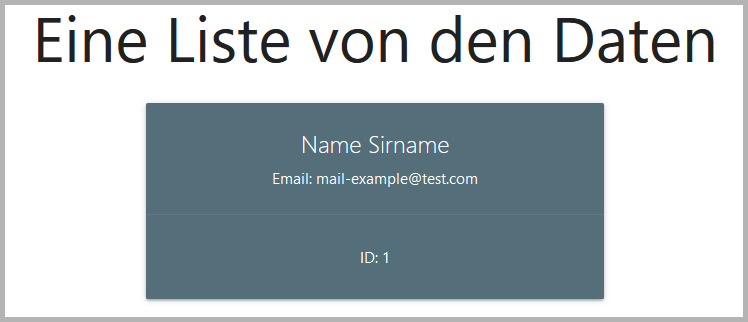
\includegraphics[width=0.8\linewidth]{images/example_page}
	\caption[Die Beispielwebseite]{Die Beispielwebseite, die mit den Umsetzungsmöglichkeiten umgesetzt werden soll.}
	\label{fig:example}
\end{figure}
Folgende Tabelle zeigt die unterschiedlichen Werte bei der Umsetzung der Beispielwebseite:
\begin{table}
	\captionof{table}[Vergleich JavaScript-Frameworks]{Vergleich von \Gls{js}-\Gls{framework}s}\label{tab:vergleich}
	\centering
	\refstepcounter{table}
	\label{center}
	\begin{tabular}{l|c|c|c|c}
		Kriterium        & Maximale Punkte & VueJS & React & Ohne Framework  \\\hline
		Design           & -                        &            \checkmark               &             \checkmark              &          \checkmark                           \\
		Entwicklungszeit & 10                         &             9              &               7            &               10                      \\
		Performanz       & 10                         &             8              &               5            &                 10                    \\
		\Gls{loc}              & 10                         &             10              &               9            &                   3                  \\
		Gesamtpunkte     & 30                         &              27             &               21            &                23                    
	\end{tabular}
\end{table}
\textbf{Kriterien:}\\\\
\textbf{Design}\\
Das Design fällt in die Wertung, da hier angegeben wird, ob die Beispiel-Website so umgesetzt werden kann oder ob die Umsetzung in diesem Design nicht möglich ist.\\\\
\newpage
\textbf{Entwicklungszeit}\\
\Gls{vue}: 40min\\
\Gls{react}: 55min\\
Ohne \Gls{framework}: 20min\\
Die Entwicklungszeit zwischen den zwei \Gls{framework}s ist sehr ähnlich. Jedoch ist zu beachten, dass bei dem VueJS-Framework bereits mit Komponenten gearbeitet worden ist und dadurch die Entwicklungszeit höher ist als notwendig. Ohne Framework war die Entwicklungszeit am kürzesten, da nichts installiert, importiert oder aufgesetzt werden musste.\\\\
\textbf{Performanz}\\
\Gls{vue}: 112ms\\
\Gls{react}: 175ms\\
Ohne \Gls{framework}: 21ms\\
Ohne Framework ist die Performanz sehr gut, da im Hintergrund keine Frameworks geladen werden müssen. Das \Gls{js} wird direkt ausgeführt. Bei VueJS und React werden viele Bibliotheken im Hintergrund geladen, wodurch die Performanz sinkt. Obwohl Komponenten bei der Umsetzung mittels VueJS verwendet worden sind, ist VueJS performanter als React.\\\\
\textbf{Lines of Code}\\
Die beiden Frameworks haben besonders gut abgeschnitten, da für die Umsetzung mit VueJS nur wenige Codezeilen geschrieben werden mussten. Durch die Funktionalität von VueJS können viele Codezeilen eingespart werden. React ist in dem Aspekt für das Projekt geeignet, da auch sehr wenige Codezeilen geschrieben werden mussten. Jedoch musste bei React deutlich mehr entwickelt werden, wodurch es nicht die vollen Punkte erreicht.
Ohne \Gls{framework} konnten weniger Punkte erreicht werden, da die Umsetzung im Vergleich nicht nur unübersichtlicher und komplizierter ist, sondern auch damit zu rechnen ist, dass die Umsetzung bei größeren Beispielen zu großen Problemen führen kann.
\newpage
\subsection{Aufbereitung der Daten}
Die Daten, welche von der REST-Schnittstelle gelesen werden, sind im \Gls{json}-Format. Dies wird genauer im Kapitel \autoref{sec:json} erklärt. Um die Daten von der REST-Schnittstelle zu bekommen, wird \Gls{axios} verwendet. Mit dieser Bibliothek kann eine \Gls{http}-Anfrage gesendet und damit die Daten von der REST-Schnittstelle ausgelesen werden. Im folgenden Code wird eine Beispiel-Anfrage gesendet:
\begin{code}{html}
	<html>
		<head>
			<!-- Import von Axios -->
			<script src="https://unpkg.com/axios/dist/axios.min.js"></script>
			<meta charset="UTF-8">
			<title>Axios-Anfrage</title>
		</head>
		<body>
			<script>
				// Anfrage an den Server um die Daten zu bekommen
				axios.get("http://localhost:3000/data").then(response => {
					//Die Daten, die zurückkommen werden in der Konsole ausgegeben
					console.log(response.data);
				})
			</script>
		</body>
	</html>
\end{code}
\captionof{listing}[HTTP-Anfrage mittels Axios]{Umsetzung einer HTTP-Anfrage mittels Axios}~\\
Die Daten, welche von der Anfrage zurückkommen, können dann verwendet werden, um \Gls{html}-Elemente zu erstellen oder zu verändern, um das \Gls{frontend} dynamisch mit den Daten zu füllen.\\Nachdem nicht alle Daten immer benötigt werden, kann bei den Anfragen die Endung verändert werden, um spezifische Daten abzufragen. Dies muss natürlich von der REST-Schnittstelle unterstützt werden. Eine Beispielanfrage für solch eine spezifische Anfrage ist wie folgt:
\begin{code}{js}
	// Hier werden z.B.: die Daten von dem Benutzer 1234 abgefragt.
	axios.get("http://localhost:3000/user/1234/infos").then(response => {
		//Die Daten, die zurückkommen werden in der Konsole ausgegeben
		console.log(response.data);
	})
\end{code}
\captionof{listing}[Axios Anfrage mit genauem Pfad]{Umsetzung einer Axios Anfrage unter Verwendung eines genauen Pfades}~\\
Die praktische Durchführung ist, wie bereits im vorherigen Kapitel besprochen, bei den Umsetzungsmöglichkeiten unterschiedlich.
\subsection{Zusammenfassung}
\label{sec:rfoster_fazit}
Nach dieser Arbeit ist die Entscheidung für eine Umsetzungsmöglichkeit einfach. \Gls{mvvm} ist genau auf webbasierte Anwendungen zugeschnitten und bei \Gls{vue} kann durch die vordefinierten Komponenten viel Zeit und Arbeit gespart werden. VueJS hat im Vergleich zu \Gls{react} den Vorteil, dass hier bereits mehr Erfahrung in der Umsetzung besteht, woraus folgt, dass VueJS die effizienteste Variante für die Umsetzung ist.
\lfoot{Linus Dehner, Michael Beier, Ryan Foster}
%!TEX root=../main.tex
\chapter{Konzept}


\lfoot{Linus Dehner}
%!TEX root=../../main.tex
\section{Frontend}
In diesem Kapitel geht es darum ein Konzept für das Frontend zu erstellen. Dabei müssen Faktoren wie beispielsweise unsere Zielgruppe, die Lehrerschaft beachtet werden. Im folgenden Kapitel werden die theoretischen Hintergründe des Konzeptes überlegt, danach werden erste Entwürfe mittels Mockups erstellt. 
\subsection{Theoretische Konzeption}
Da die Zielgruppe \enquote{Lehrer} nicht gleichaltrig ist, sondern die darin enthaltenen Menschen ein Alter von 25 bis 65 Jahren haben gibt es keine Literatur zur \enquote{perfekten Usability für Lehrpersonal}. Daher richten wir uns nach dem Buch \enquote{Don't Make Me Think: A Common Sense Approche to Web Usability} von Steve Krug und an dem Buch \enquote{101 UX Principles} von Will Grant. Um eine gute Usability für die Lehrer des TGMs zu gewährleisten werden wir den Prozess der Entwicklung streng in Kontakt zu Lehrern begleiten und das Produkt auch mit nicht Technik affinen Menschen testen.  
\subsection{Visuelle Konzeption}
\paragraph{Login-Seite}
~\\
Wie man auf der Abbildung 6.1 sehen kann ist die Login-Seite sehr schlicht gehalten. Neben dem Schriftzug \enquote{Refundable} soll das Formular zum einloggen sein. Da die Plattform nur für das Personal des TGMs zugänglich sein soll, wird bei der Eingabe der E-Mail Adresse automatisch eine \enquote{@tgm.ac.at} Adresse gefordert. Wird der \enquote{Passwort vergessen?} Link betätigt, soll automatisch auf die Seite des TGMs verwiesen werden, da wir über LDAP die Daten der Lehrer abrufen. Bei der Eingabe von validen Daten und des betätigen des \enquote{Anmelden} Buttons wird der Benutzer auf die Startseite weitergeleitet.
\begin{figure}[H]
	\centering
	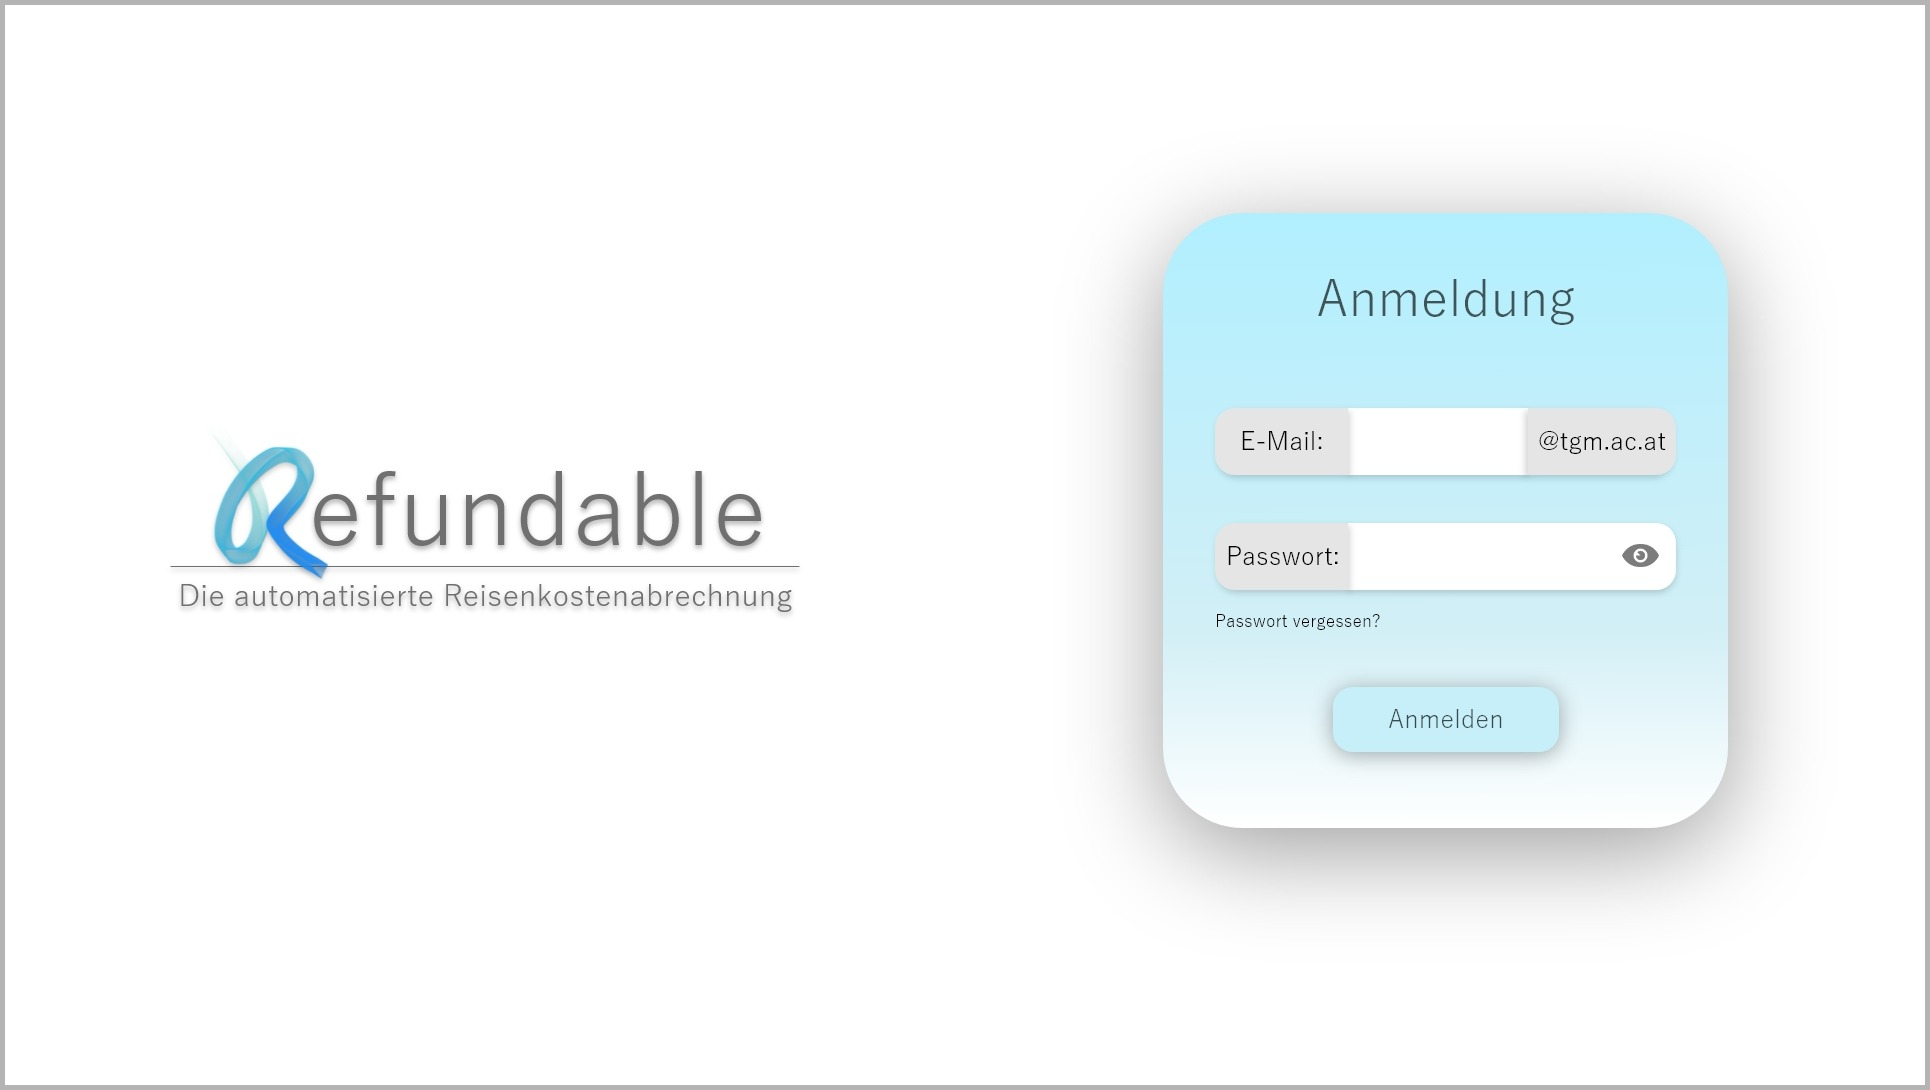
\includegraphics[width=1\linewidth]{images/Mockup-Startseite}
	\caption[Mockup Login]{Das Mockup der Login Seite}
	\label{fig:mockupLogin}
\end{figure}
\paragraph{Startseite}
~\\

\begin{figure}[H]
	\centering
	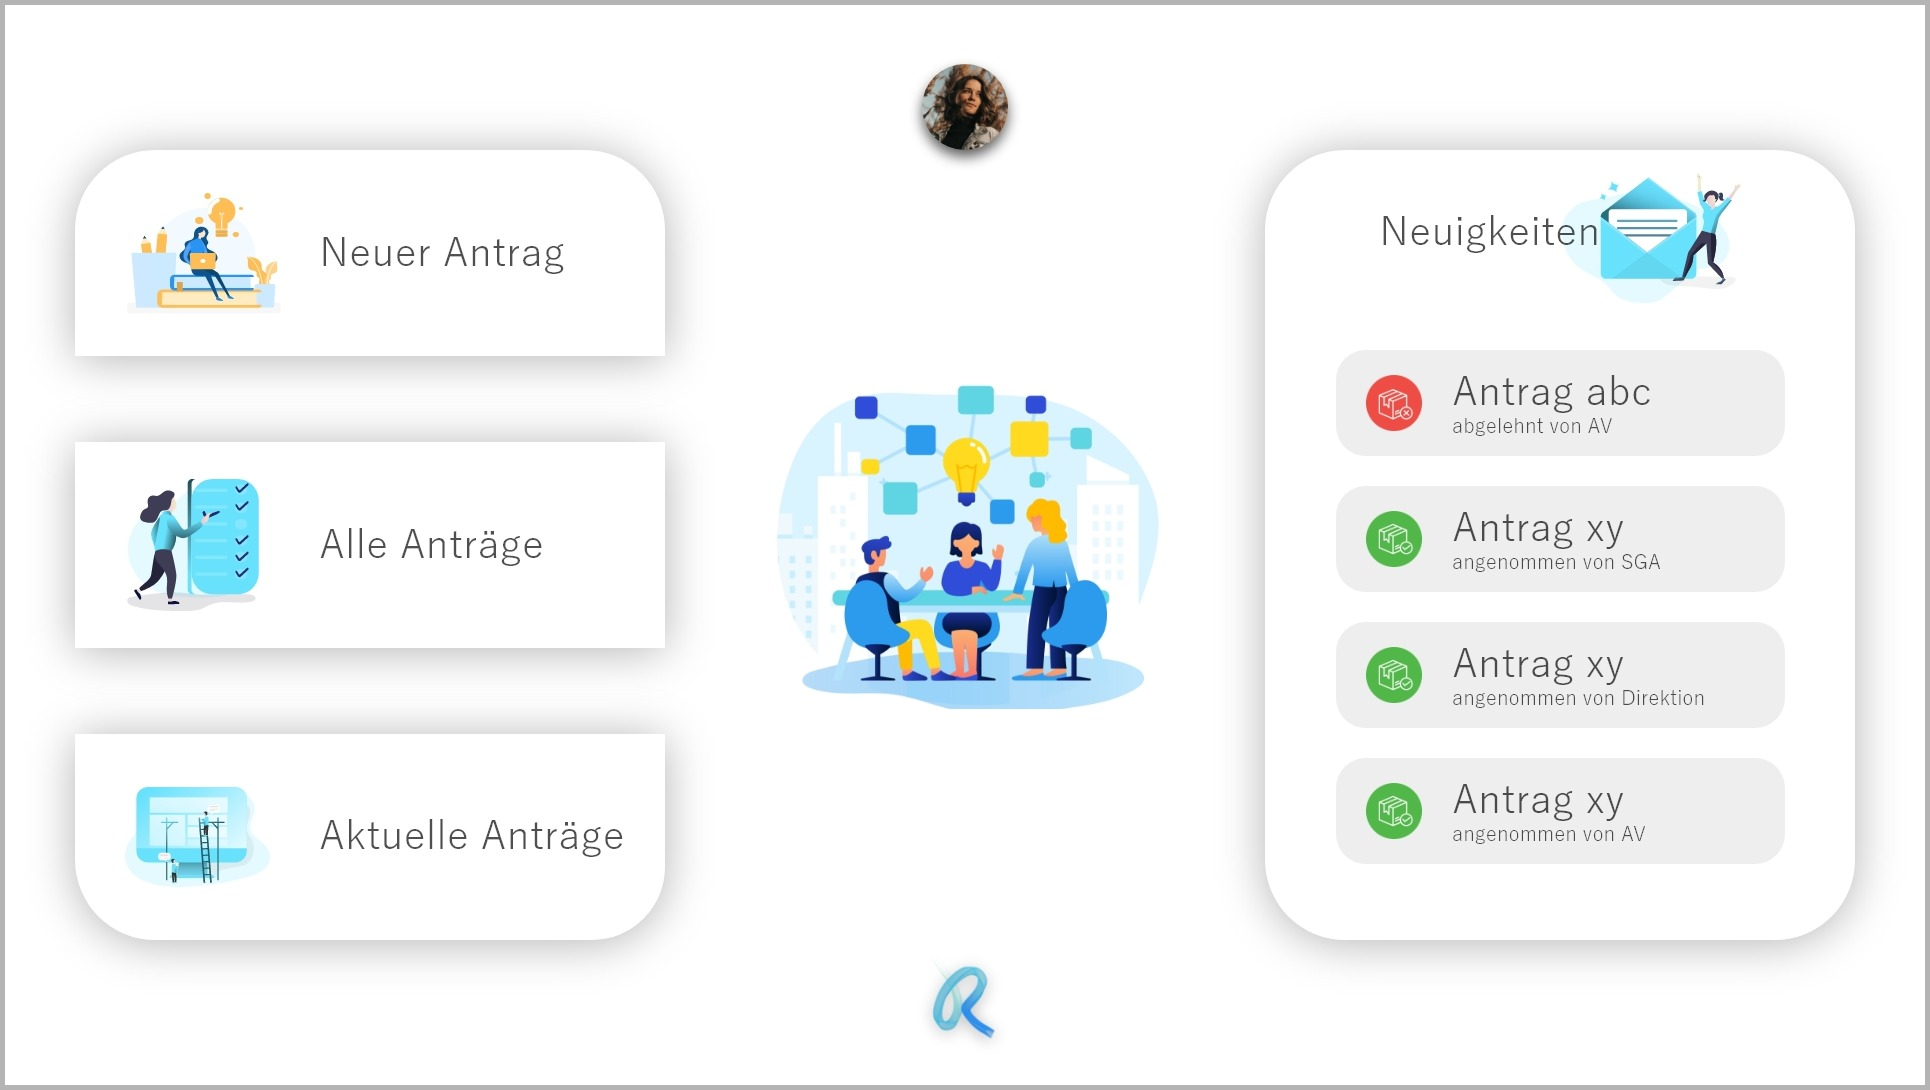
\includegraphics[width=1\linewidth]{images/Mockup-Startseite-eingeloggt}
	\caption[Mockup Startseite]{Das Mockup der Startseite, nachdem man sich eingeloggt hat}
	\label{fig:mockupStart}
\end{figure}
\paragraph{Neuer Antrag}
~\\

\begin{figure}[H]
	\centering
	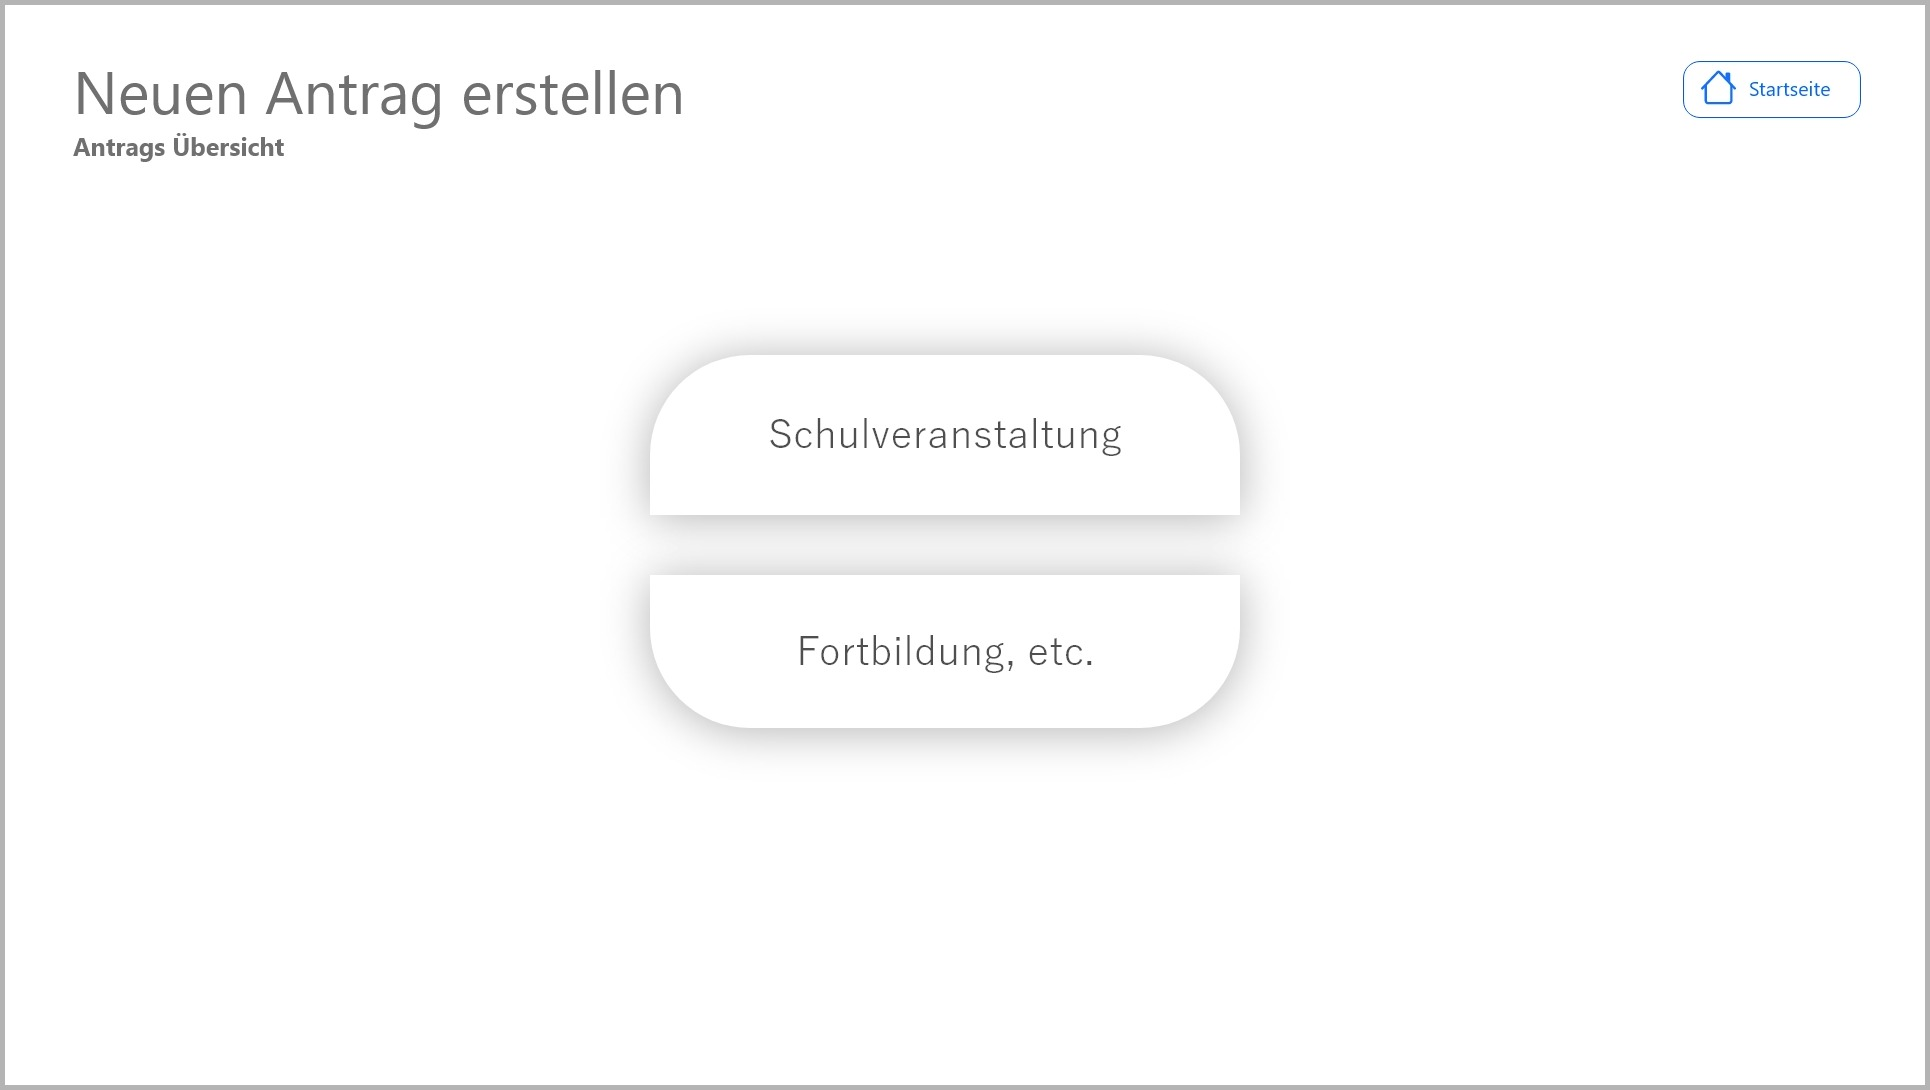
\includegraphics[width=1\linewidth]{images/Mockup-Neuer-Antrag}
	\caption[Mockup neuer Antrag]{Das Mockup der Seite, auf der man eine Antragsart auswählen kann}
	\label{fig:mockupNeu}
\end{figure}
\paragraph{Antrag ausfüllen}
~\\

\begin{figure}[H]
	\centering
	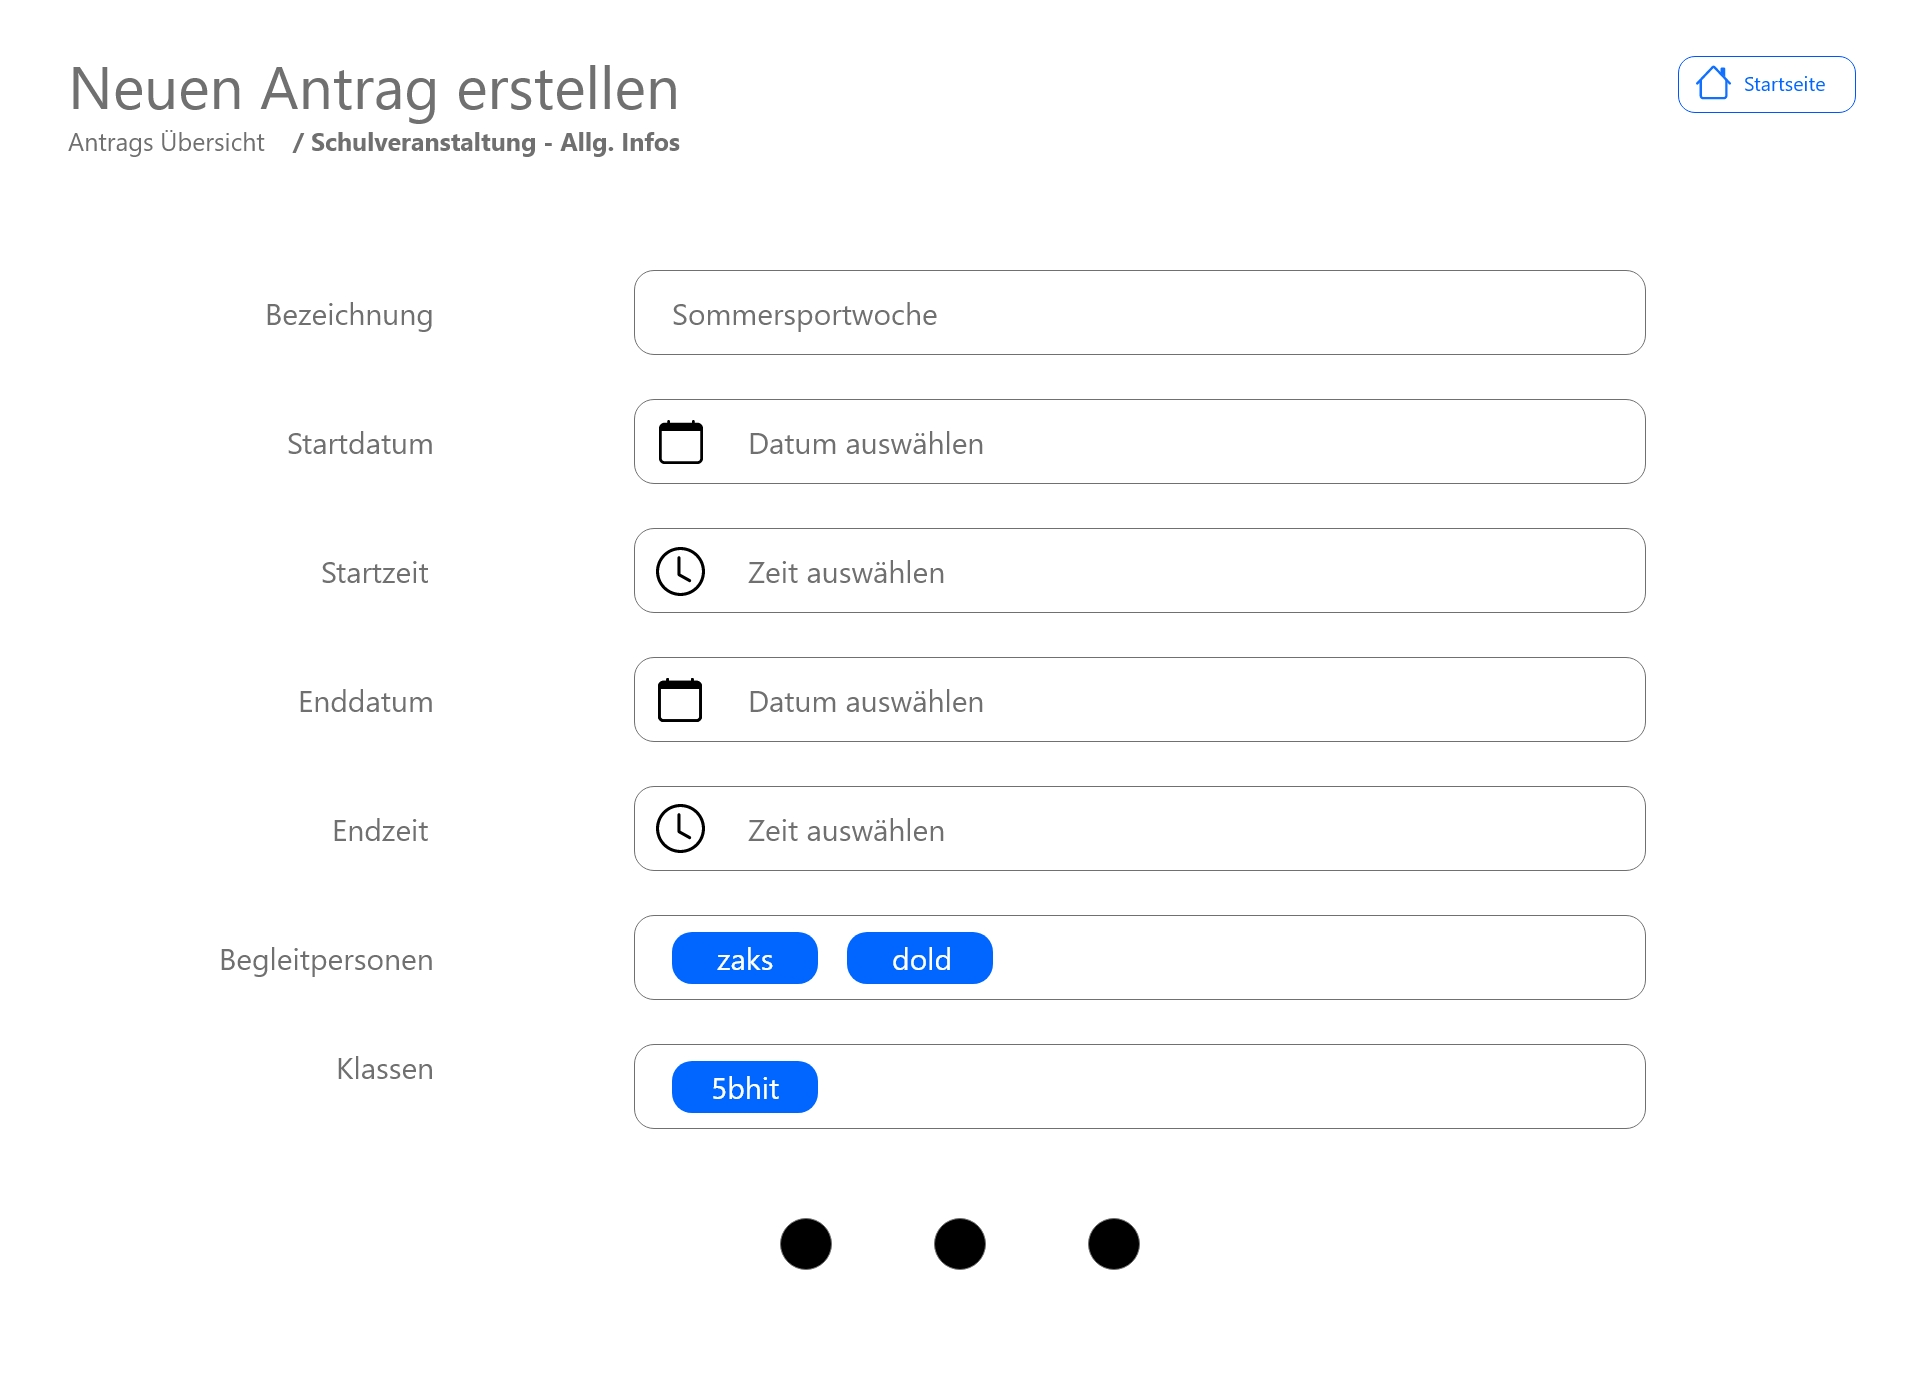
\includegraphics[width=1\linewidth]{images/Mockup-Antrag-erstellen}
	\caption[Mockup Antrag erstellen]{Das Mockup zum erstellen einer neuen Schulveranstaltung}
	\label{fig:mockupErstellen}
\end{figure}
\paragraph{Ansicht Alle Anträge}
~\\

\begin{figure}[H]
	\centering
	\includegraphics[width=1\linewidth]{images/Mockup-Alle-Anträge}
	\caption[Mockup Alle Anträge]{Das Mockup, welches alle Anträge einer gewissen Person veranschaulicht}
	\label{fig:mockupAlle}
\end{figure}
\paragraph{Ansicht Aktive Anträge}
~\\

\begin{figure}[H]
	\centering
	\includegraphics[width=1\linewidth]{images/Mockup-Aktive-Anträge}
	\caption[Mokup aktive Anträge]{Das Mockup, welches alle aktiven Anträge einer gewissen Person veranschaulicht}
	\label{fig:mockupAktive}
\end{figure}
\paragraph{Administrator Ansicht}
~\\

\begin{figure}[H]
	\centering
	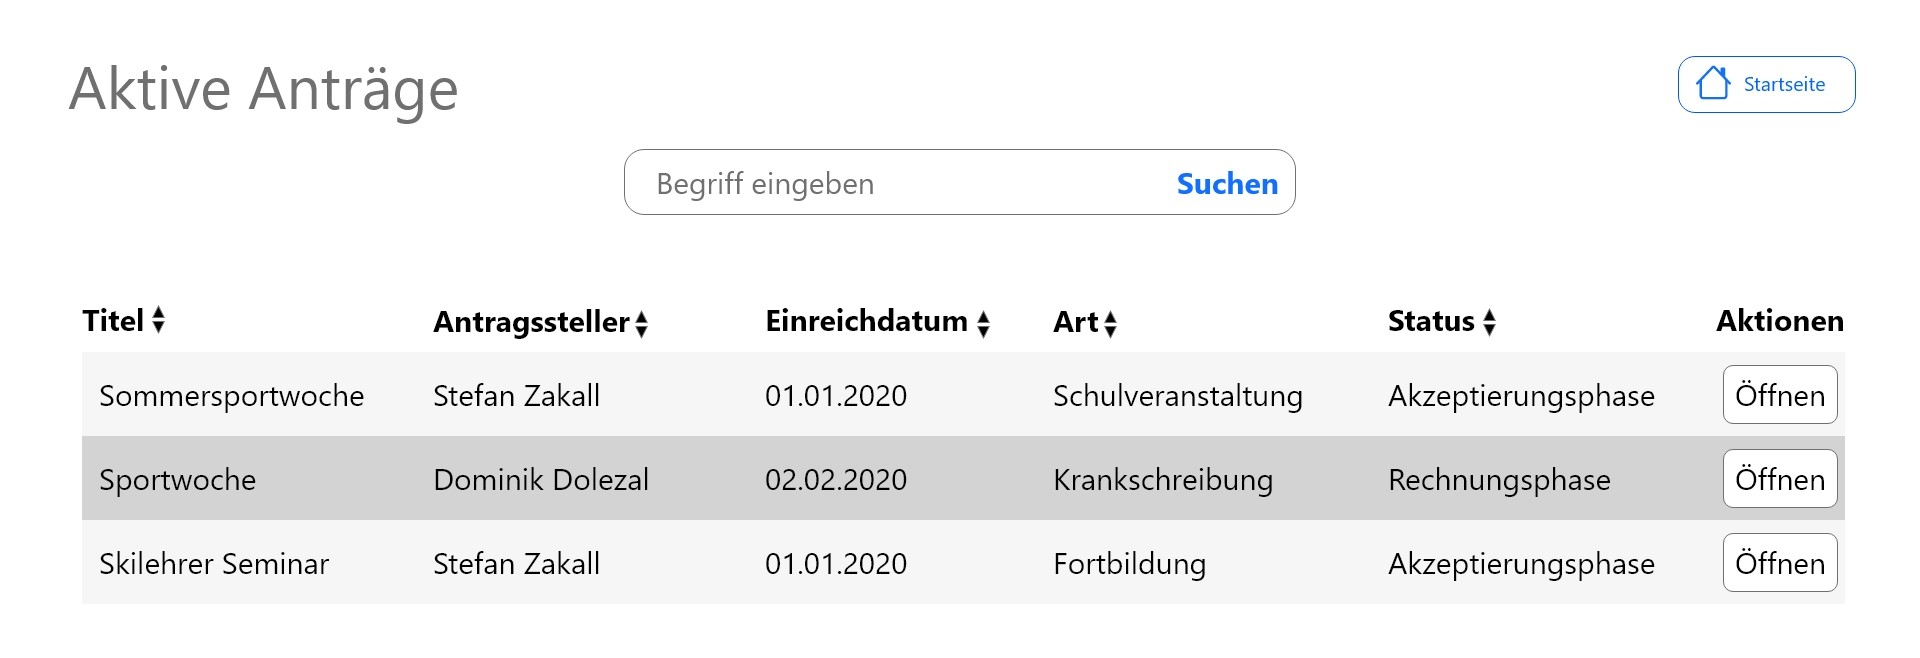
\includegraphics[width=1\linewidth]{images/Mockup-Admin}
	\caption[Mockup Adminansicht]{Das Mockup, der Admin Ansicht, zum akzeptieren und ablehnen von Anträgen}
	\label{fig:mockupAdmin}
\end{figure}
\paragraph{Antragsansicht}
~\\

\begin{figure}[H]
	\centering
	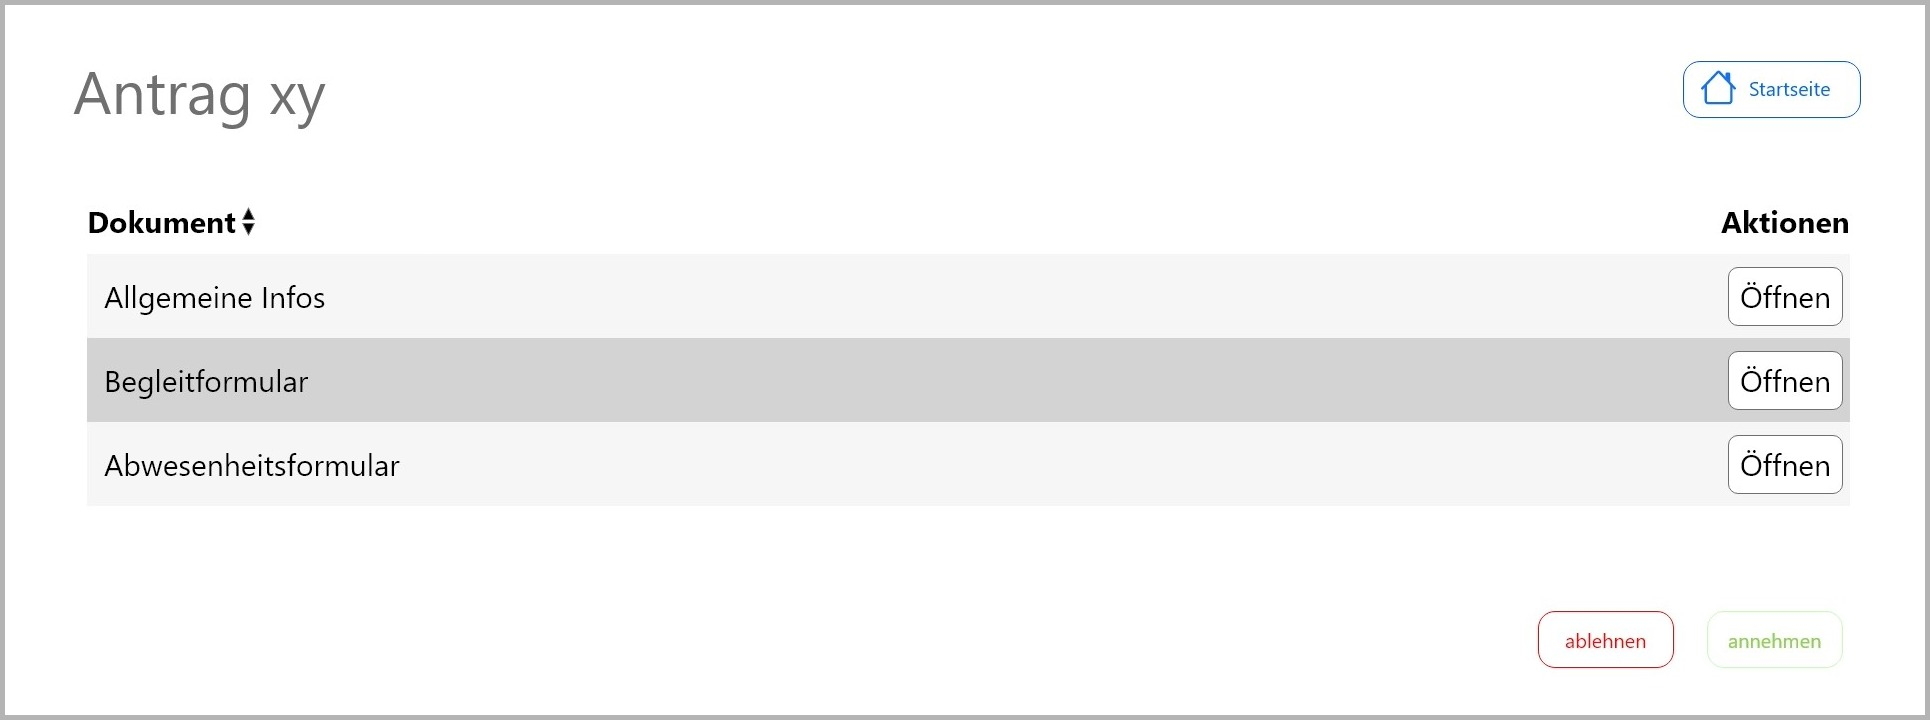
\includegraphics[width=1\linewidth]{images/Mockup-Antragsansicht}
	\caption[Mockup Antragsansicht]{Das Mockup, welches einen eingereichten Antrag veranschaulicht}
	\label{fig:mockupAntrag}
\end{figure}
\lfoot{Michael Beier}
%!TEX root=../../main.tex

\section{Backend und Infrastruktur}
\subsection{Einleitung}
Der Anspruch an die Infrastruktur und an das Backend besteht darin, die Software als ganzes zu steuern und zu erhalten. Die Infrastruktur muss einfach zu aufbauen und zu starten sein. Die folgenden Kapiteln erläutern nach der generellen Analyse von Lösungsmöglichkeiten im \autoref{chap:backendsota} nun einen ausgearbeiteten Plan, wie die später folgende Implementierung aussehen soll. Hierfür werden Graphiken oder Tabelle verwendet. Sie sollen ausreichend Informationen über Abläufe oder verschiedene Funktionalität vorgeben, um diese entsprechend daraufhin zu implementieren. Des Weiteren sollen die genormten Diagrammarten dazu dienen das komplexe Backend und die Infrastruktur einfach und übersichtlich darzustellen, um speziell die Schnittstellenherausforderungen verständlich zu machen.
\subsection{Infrastruktur}
Die Infrastruktur enthält jegliche Dienste und Anwendungen, welche von der Software in der Projektumgebung benötigt werden. Um diese Dienste mit einfach aufbauen zu können wird eine Virtualisierung über Container mittels Docker umgesetzt. Diese virtuellen Instanzen verbunden in einem Docker-Compose Stack werden über ein eigenes Skript gesteuert.
\subsubsection{Docker Stack}
\begin{figure}[H]
	\centering
	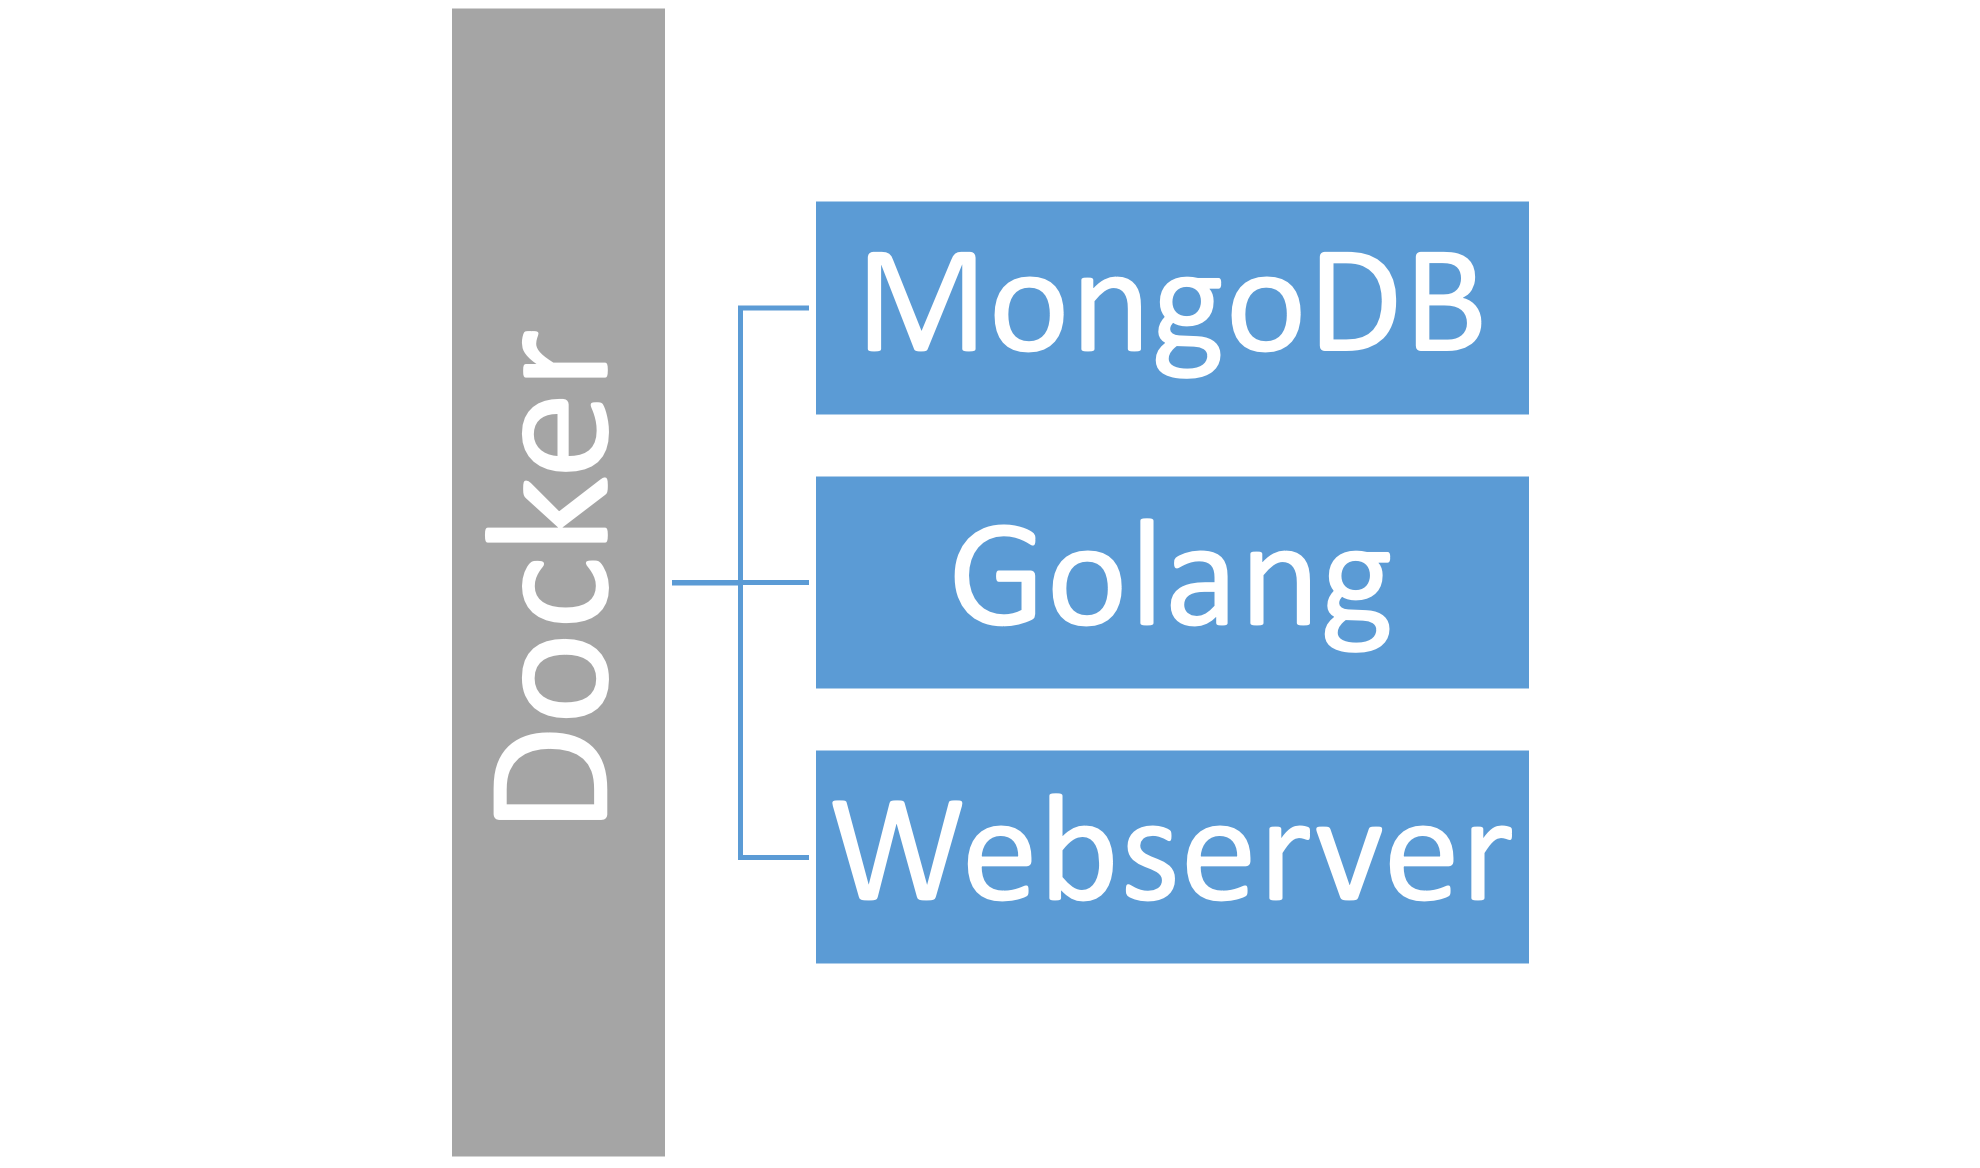
\includegraphics[width=\linewidth]{images/mbeier_konzept/docker-stack}
	\caption[Docker-Compose Stack]{Übersicht über die Container des Docker-Compose Stack}
	\label{fig:docker-stack}
\end{figure}

\newpage

Diese in Docker Container befindlichen Dienste und Anwendungen werden benötigt um die Software funktionsfähig bereitzustellen. Der automatische Aufbau dieser Container-Infrastruktur geschieht auf Basis einer Docker-Compose Konfiguration automatisch. \\

Docker Container stellen eigene Umgebungen dar, welche nach dem stoppen oftmals vollständig zerstört und gelöscht werden. Die Daten, auf die die Software und auch die anderen Anwendungen zugreifen müssen, sind jedoch über die Lebenszeit eines Docker Container darüber hinaus zu persistieren. Um dies garantieren zu können, werden Volumes in die Container eingehängt, so dass die Daten prinzipiell außerhalb der Container gespeichert wird und nur von außen in die Umgebungen eingehängt werden. Dies ist bei dem MongoDB Container erforderlich, um die Daten, welche in der Datenbank gespeichert werden, permanent zu speichern. Ebenso ist es erforderlich die generierten Dateien des Golang-Backends zu persistieren, um auf diese später wieder zugreifen zu können. Auch werden im Backend diverse gleichbleibende Passphrasen, beispielsweise zum Signieren von Tokens, auf die gleiche Art und Weise gespeichert. \\

Die Zugangsdaten für den Nutzeraccount, welche beim Installieren abgefragt werden (siehe \autoref{fig:install}), der Datenbank werden über Dockers Secrets-Management sowohl in den Datenbank-, als auch in den Golang-Container, damit sich dieser zur Datenbank verbinden kann, eingehängt. In der Datenbank müssen initial neben den Datenbanknutzern auch die Datenbankinstanz selbst angelegt werden. Dies geschieht über ein eigenes zum Start ausführendes Skript. \\

Das Frontend selbst besteht aus zwei Ebenen. Zu Beginn am Start wird das Frontend selbst kompiliert und installiert. Hierfür gibt es einen eigenen Container, der hierfür eine Umgebung bietet. Danach wird der eigentliche Webserver-Container gestartet und die zuvor kompilierten Dateien werden in den neuen Container kopiert. Ebenfalls wird eine angelegte Konfigurationsdatei, die den Webserver Dienst weitergehend konfiguriert, in das entsprechende Verzeichnis hinzugefügt.\\

% ToDo HTTPS Certificates

\newpage

\subsubsection{Steuerungsskript}

Das Steuerungsskript ermöglicht die genaue und einfache Steuerung der Infrastruktur.
Hierfür implementiert das Steuerungsskript folgende Submethoden mit entsprechenden Abläufen und Funktionalität:\\

\textbf{Installationsvorgang:}

\begin{figure}[H]
	\centering
	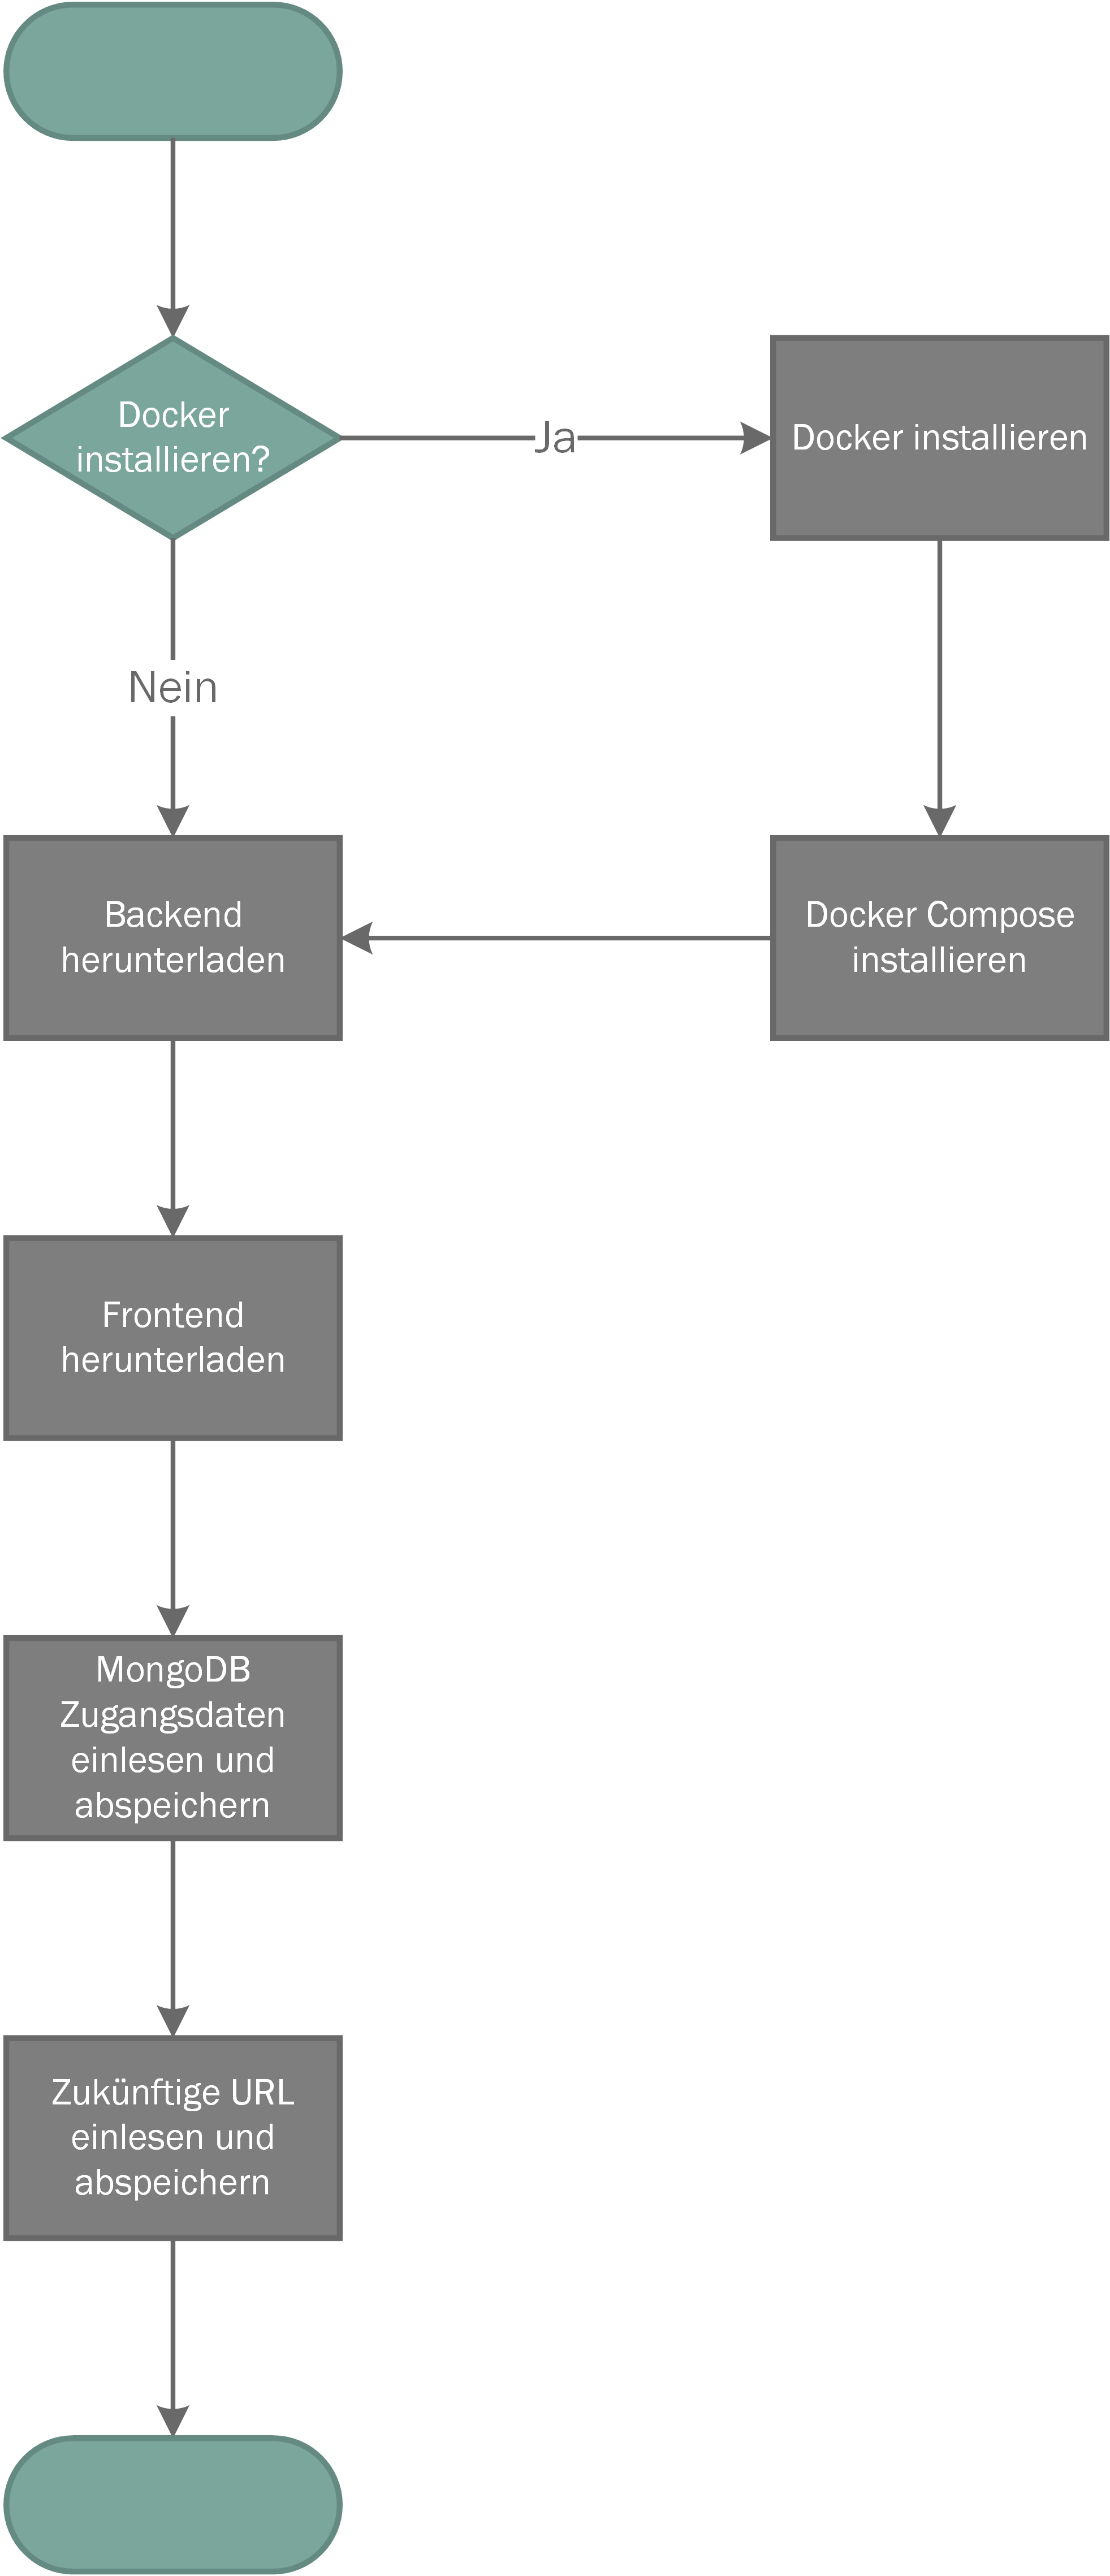
\includegraphics[width=0.5\linewidth]{images/mbeier_konzept/Install}
	\caption[Flussdiagramm über den Installationsvorgang]{Flussdiagramm über den Installationsvorgang}
	\label{fig:install}
\end{figure}

\newpage

Die Idee hinter der Etablierung eines Installationsvorganges soll die Einfachheit der Steuerung der Software hervorheben. Das Install-Repository beinhaltet hierbei lediglich eine grundlegende Ordnerstruktur und das Steuerungsskript selbst. Durch den Installationsvorgang werden die restlichen benötigten Daten automatisch heruntergeladen und installiert.

~\\~\\~\\
\textbf{Startvorgang:}

\begin{figure}[H]
	\centering
	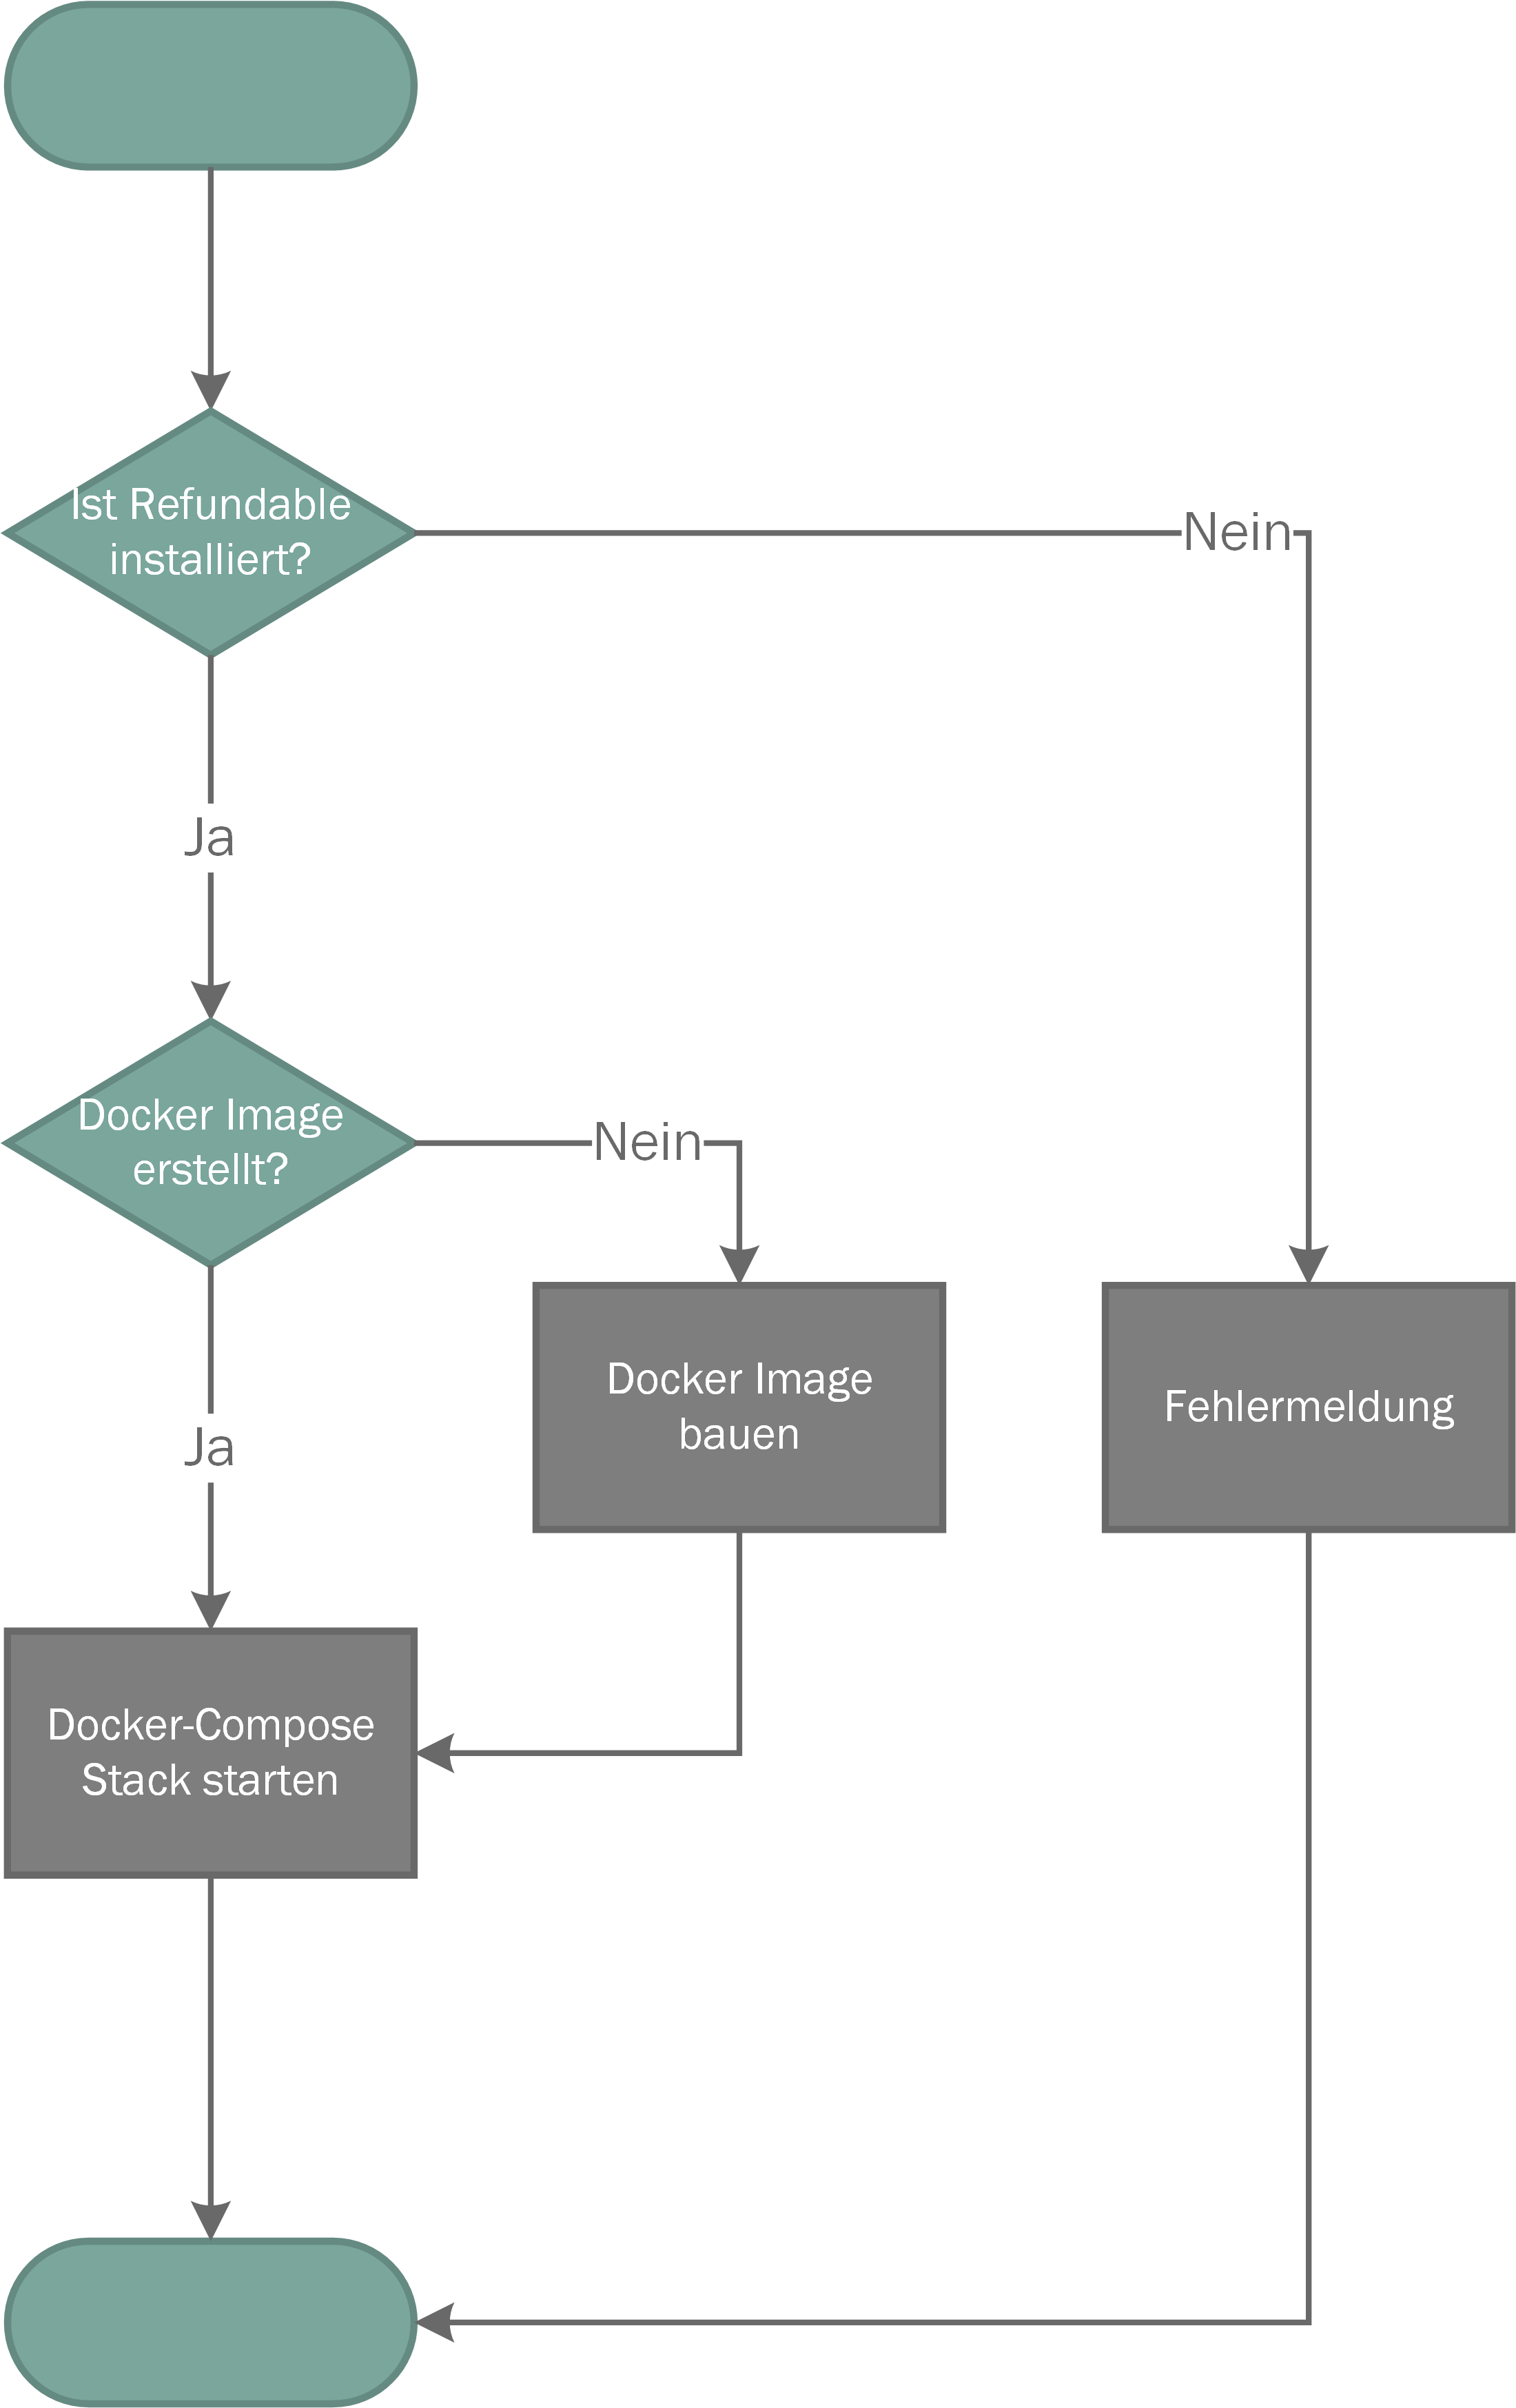
\includegraphics[width=0.5\linewidth]{images/mbeier_konzept/Start}
	\caption[Flussdiagramm über den Startvorgang]{Flussdiagramm über den Startvorgang}
	\label{fig:start}
\end{figure}

Der Startvorgang baut die Docker-Images, sofern diese noch nicht vorhanden sind, grundlegend auf Basis der installierten Dateien auf und startet daraufhin den gesamten Stack auf einmal. Voraussetzung hierfür ist, dass der Installationsvorgang bereits abgeschlossen ist und die heruntergeladenen Dateien vorhanden sind.

\newpage  

\textbf{Stoppvorgang:}

\begin{figure}[H]
	\centering
	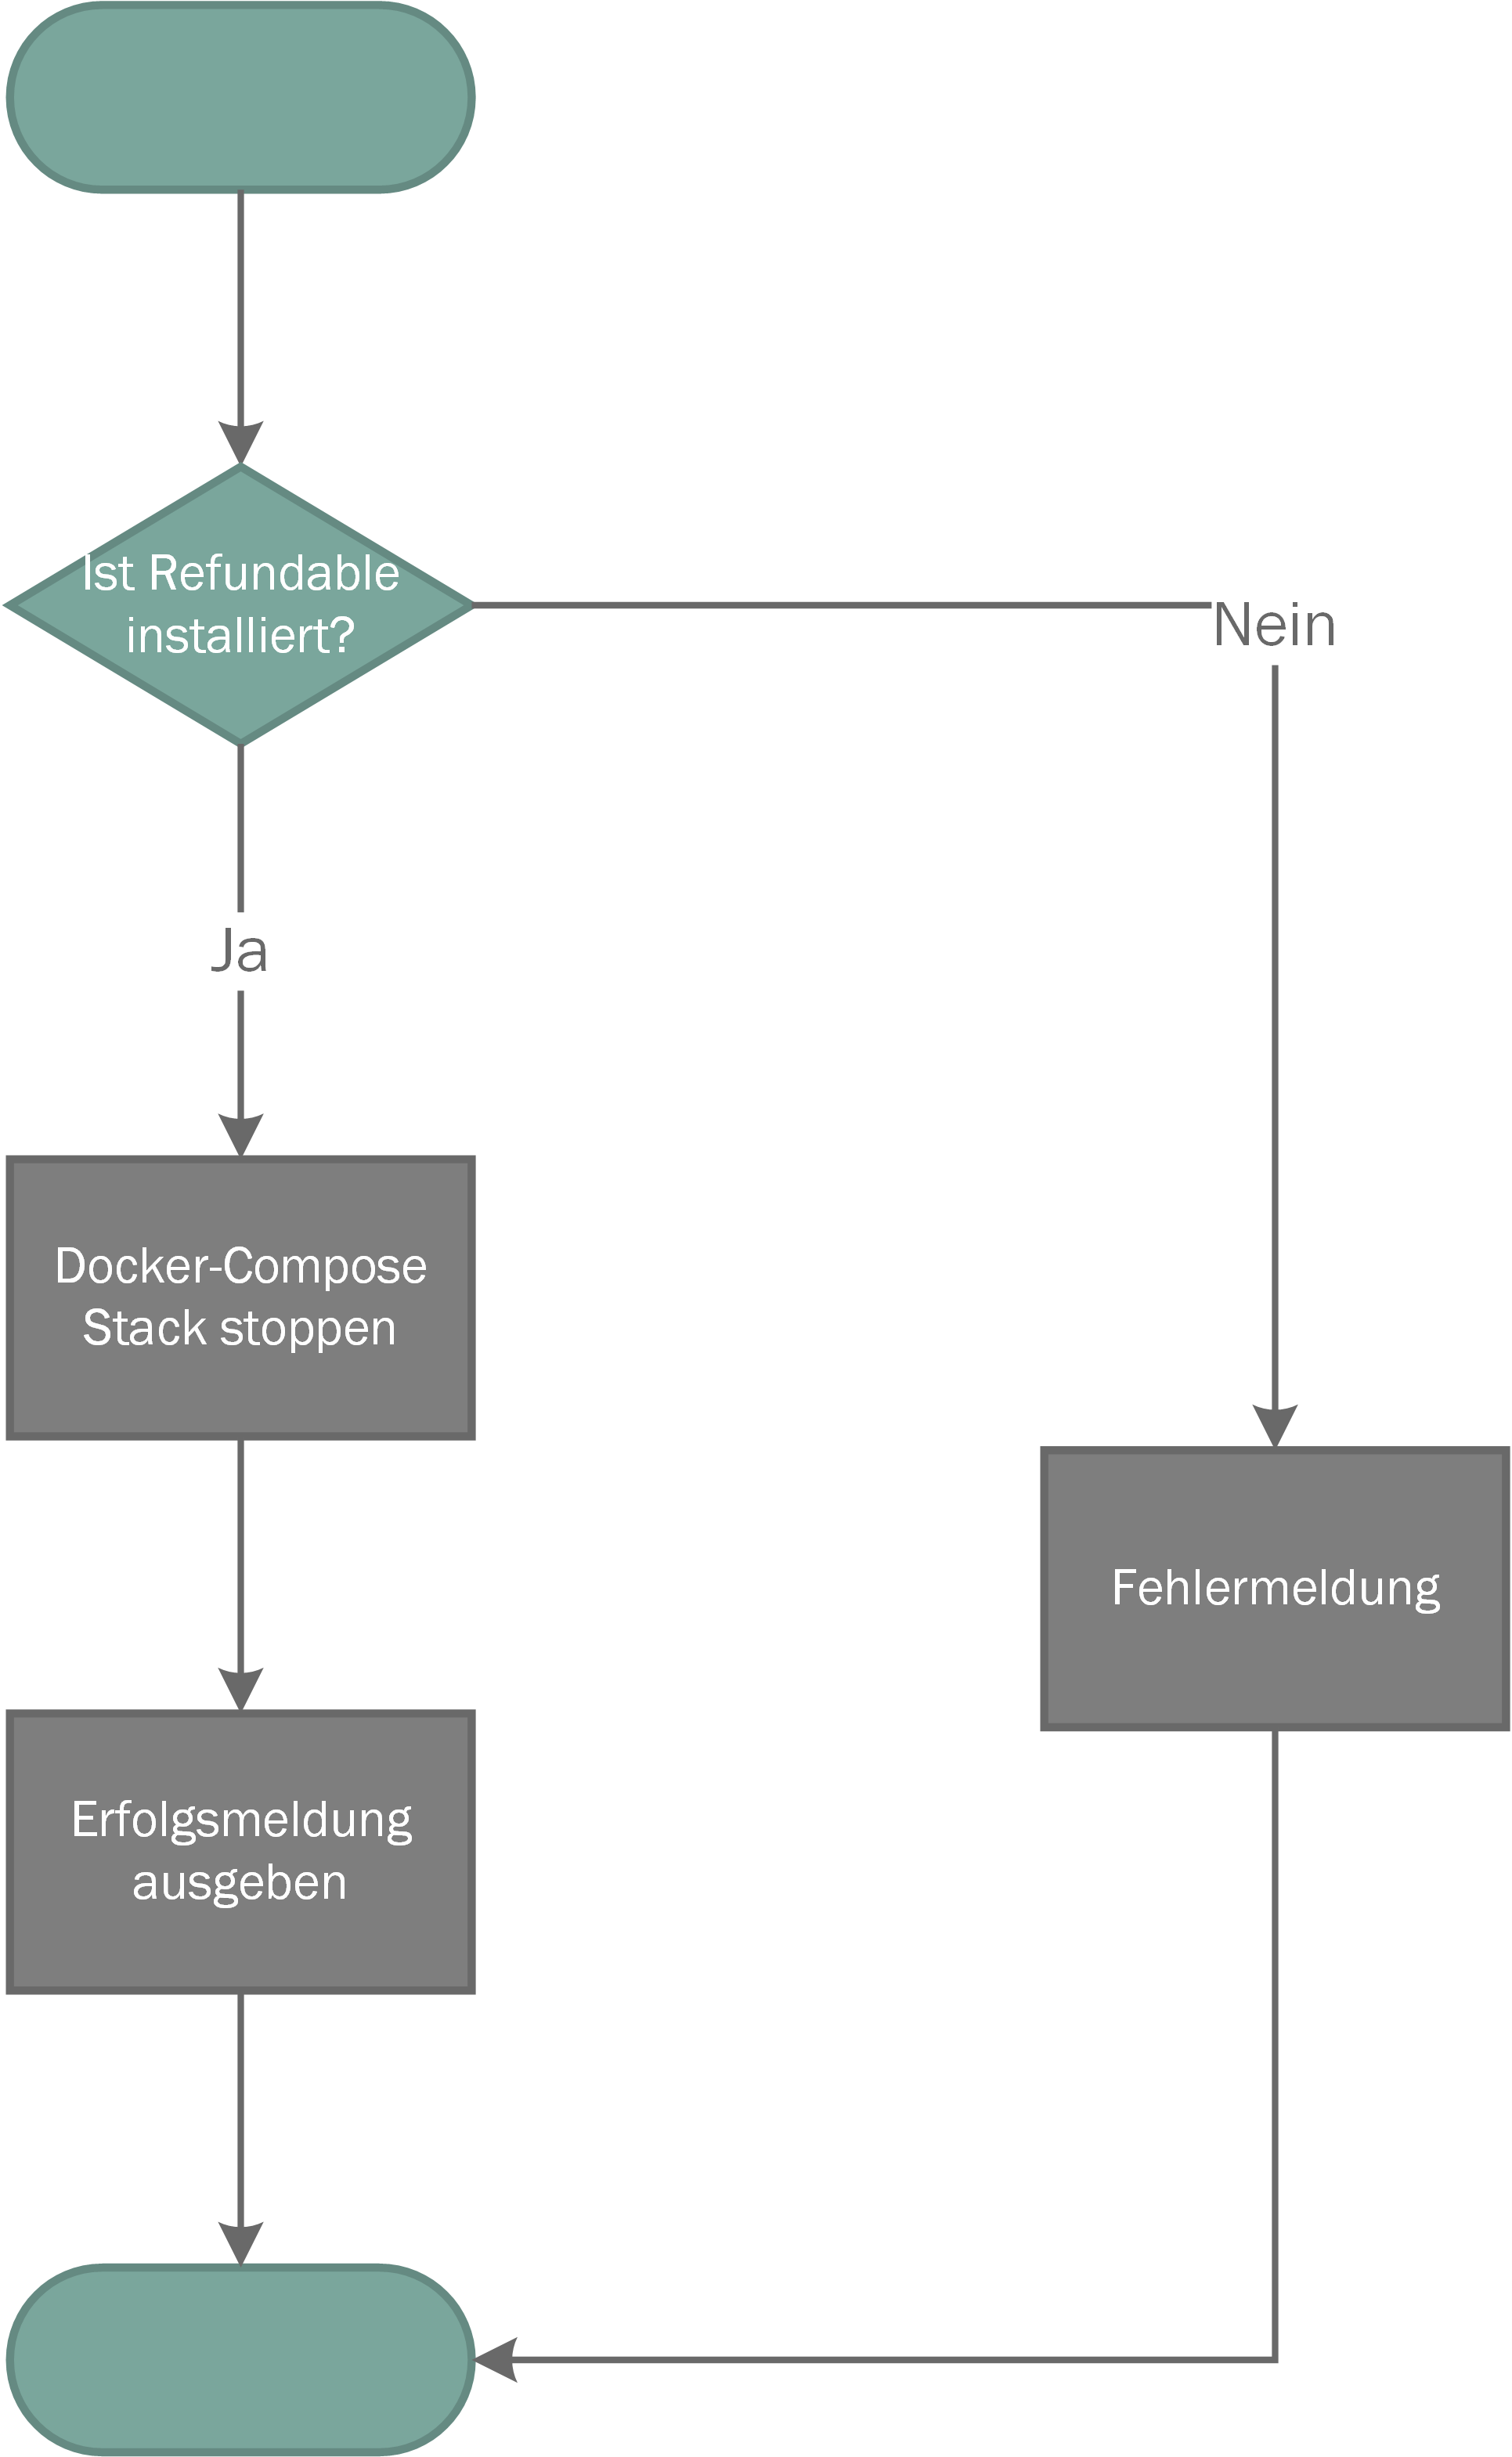
\includegraphics[width=0.5\linewidth]{images/mbeier_konzept/Stop}
	\caption[Flussdiagramm über den Stoppvorgang]{Flussdiagramm über den Stoppvorgang}
	\label{fig:stop}
\end{figure}

~\\
Der Stoppvorgang stoppt die laufenden Docker-Container und entfernt diese aus der Docker Umgebung. Dies führt dazu, dass garantiert wird, dass sich die wieder neu aufbauende Umgebung tatsächlich neu ist, und nicht nur eine alte Instanz wiederverwendet wird.

\newpage

\textbf{Neustartvorgang:}

\begin{figure}[H]
	\centering
	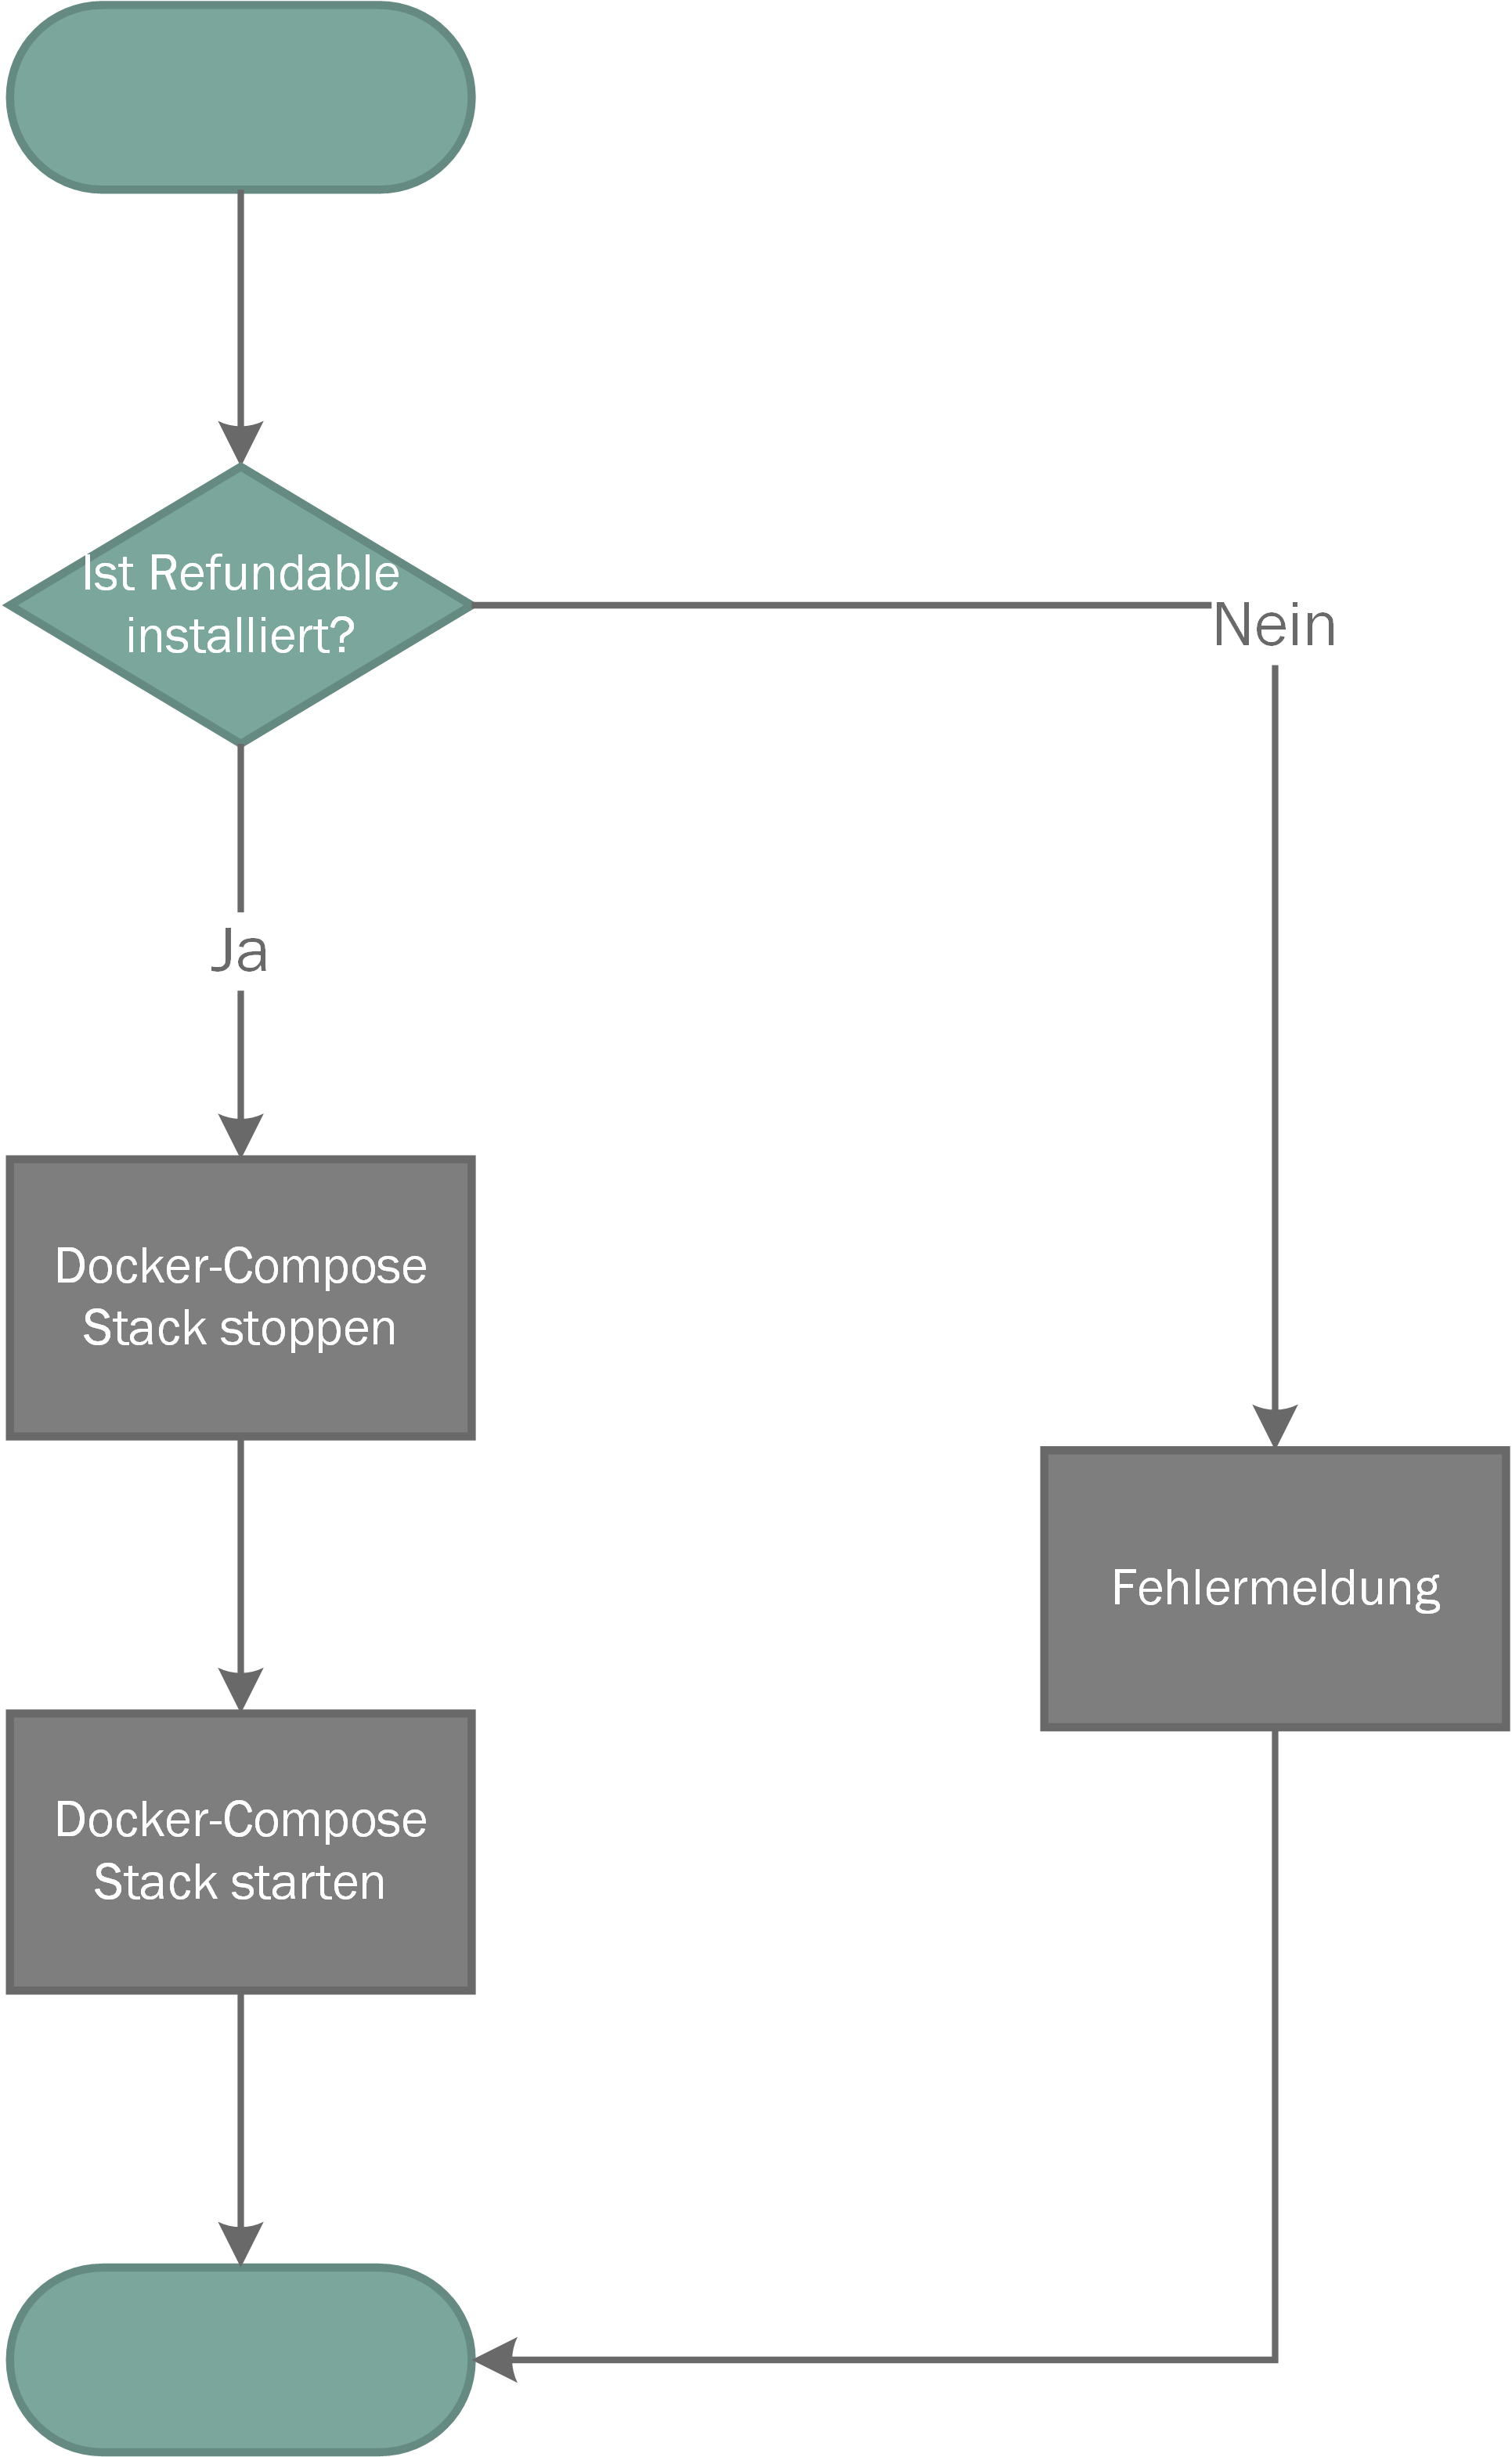
\includegraphics[width=0.5\linewidth]{images/mbeier_konzept/Restart}
	\caption[Flussdiagramm über den Neustartvorgang]{Flussdiagramm über den Neustartvorgang}
	\label{fig:restart}
\end{figure}
~\\
Der Neustartvorgang kombiniert den Start- und Stoppvorgang und führt diese beiden auf einmal aus. Er wird hauptsächlich dafür genutzt, um neue Konfigurationen, welche nur beim Start des Systems eingelesen werden, von der Software übernehmen zu lassen.

\newpage

\textbf{Aktualisierungsvorgang:}

\begin{figure}[H]
	\centering
	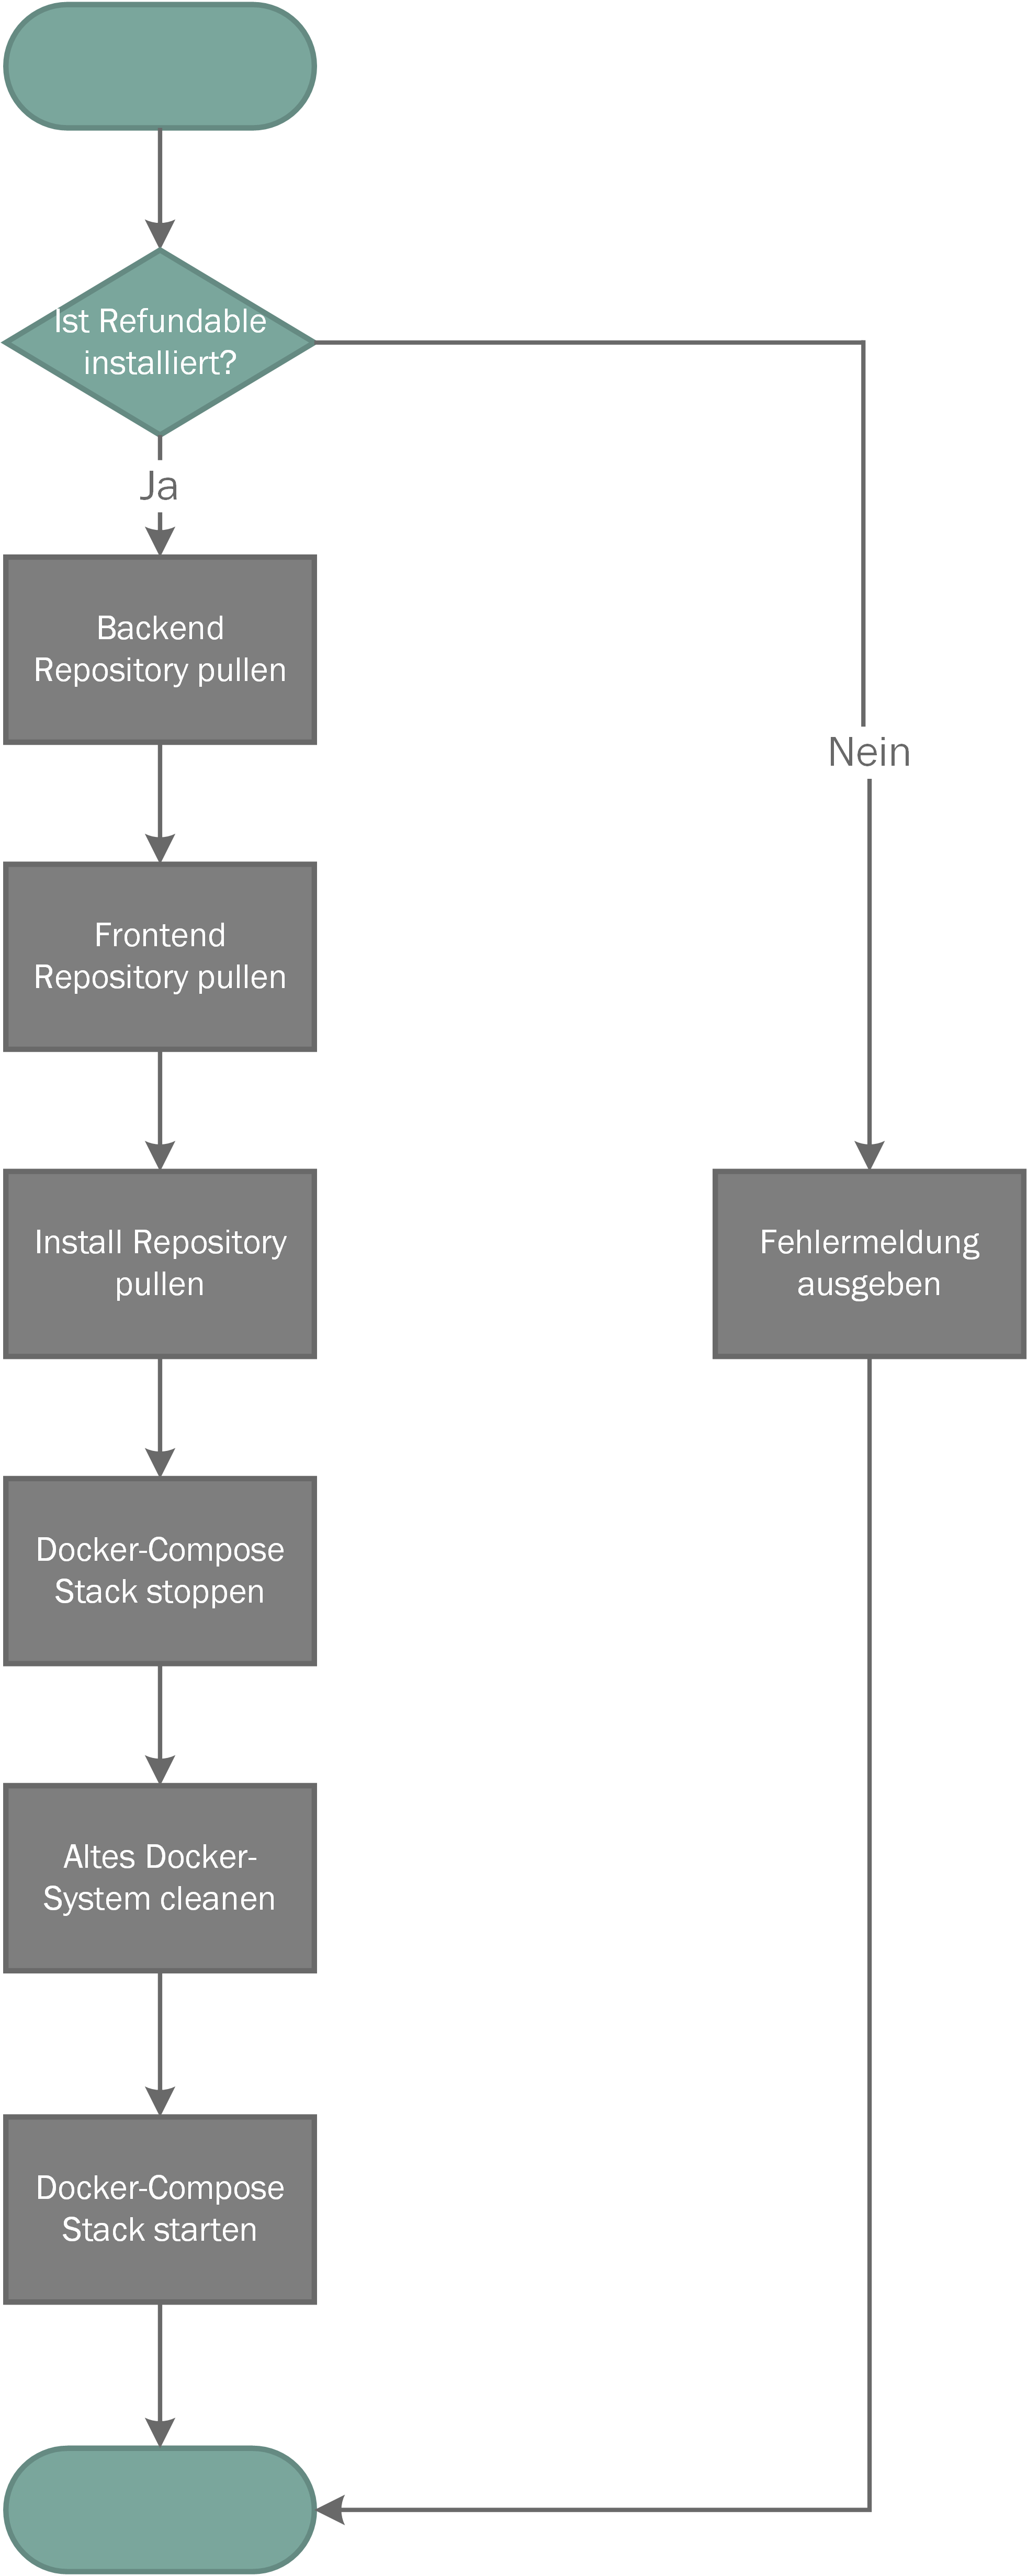
\includegraphics[width=0.47\linewidth]{images/mbeier_konzept/Update}
	\caption[Flussdiagramm über den Aktualisierungsvorgang]{Flussdiagramm über den Aktualisierungsvorgang}
	\label{fig:update}
\end{figure}
~\\
Der Aktualisierungsvorgang ist dem Installationsvorgang sehr ähnlich. Da es sich bei den installierten Dateien um solche aus Git-Repositories handelt, können diese auch einfach aktualisiert werden. Daraufhin wird nur noch ein Neustart des Systems durchgeführt.

\newpage

\textbf{Bereinigungsvorgang:}

\begin{figure}[H]
	\centering
	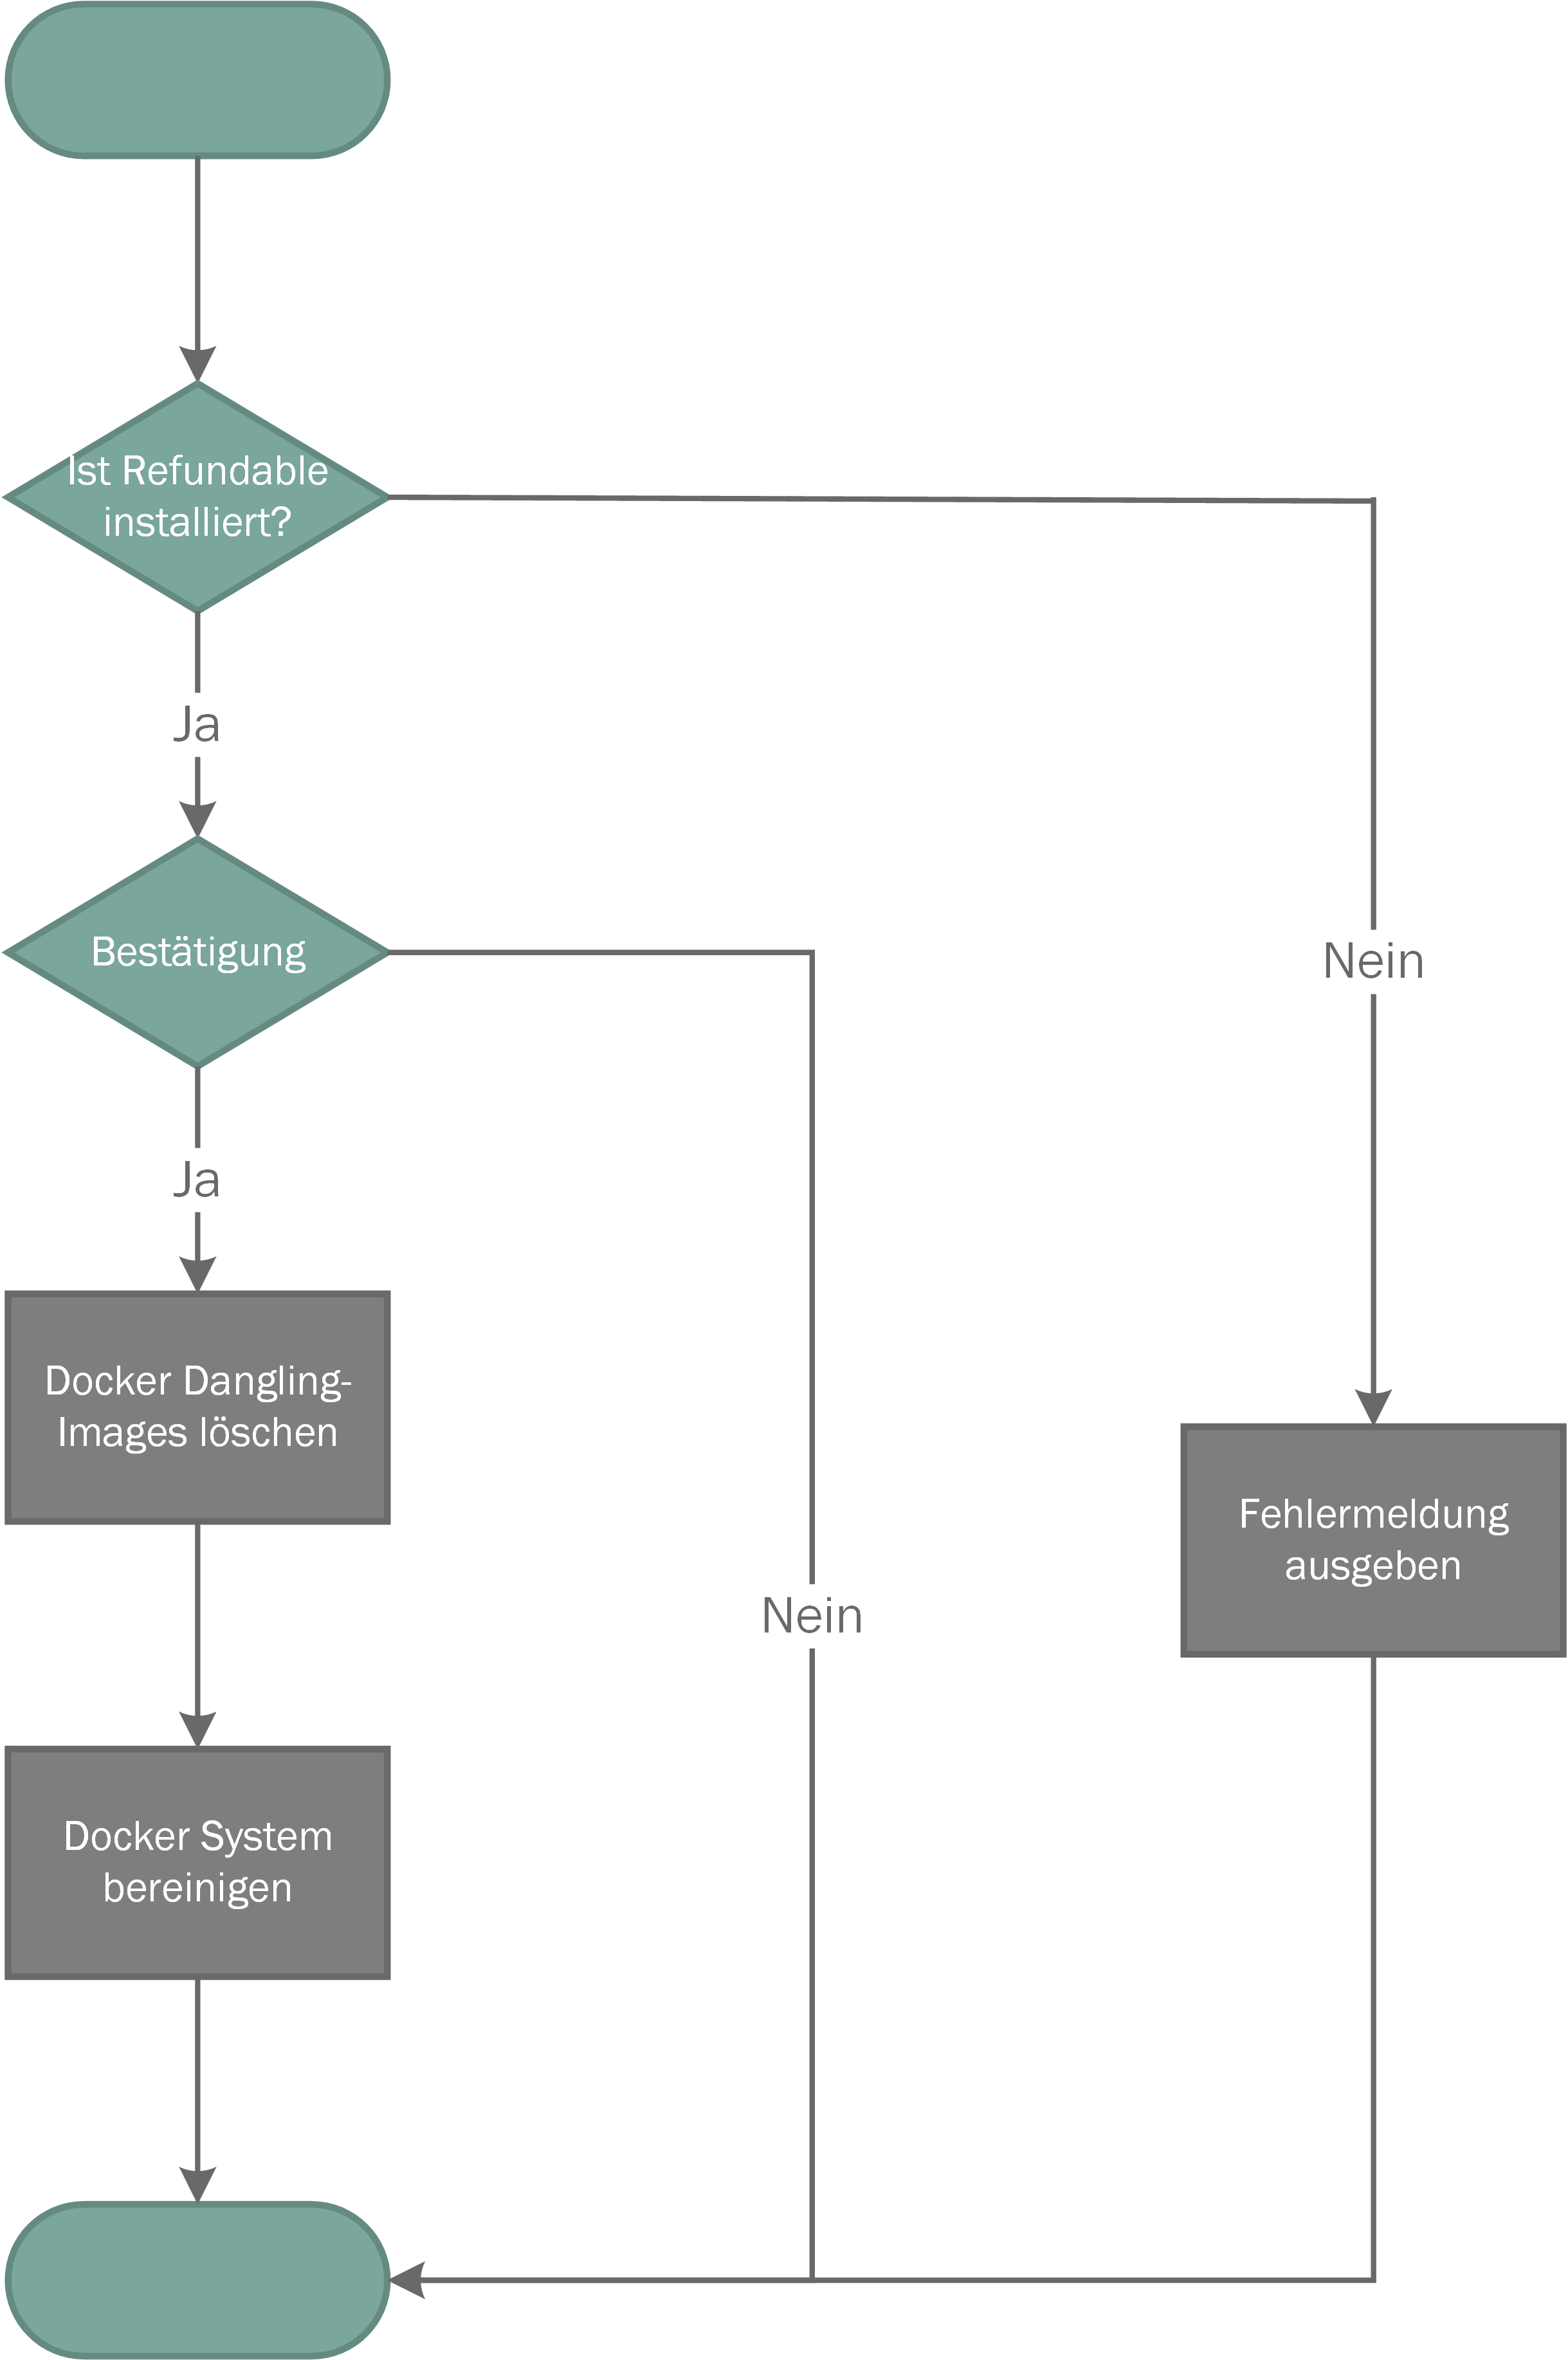
\includegraphics[width=0.55\linewidth]{images/mbeier_konzept/Clean}
	\caption[Flussdiagramm über den Bereinigungsvorgang]{Flussdiagramm über den Bereinigungsvorgang}
	\label{fig:clean}
\end{figure}
~\\
Der Bereinigungsvorgang nutzt die Docker Funktionen zum Löschen von nicht mehr benutzten Docker Images (Dangling Images). Nachdem werden die danach nicht mehr benutzten Ressourcen über die entsprechende Docker-Funktion aus dem System und der Docker Umgebung entfernt.

\newpage

\textbf{Deinstallation:}

\begin{figure}[H]
	\centering
	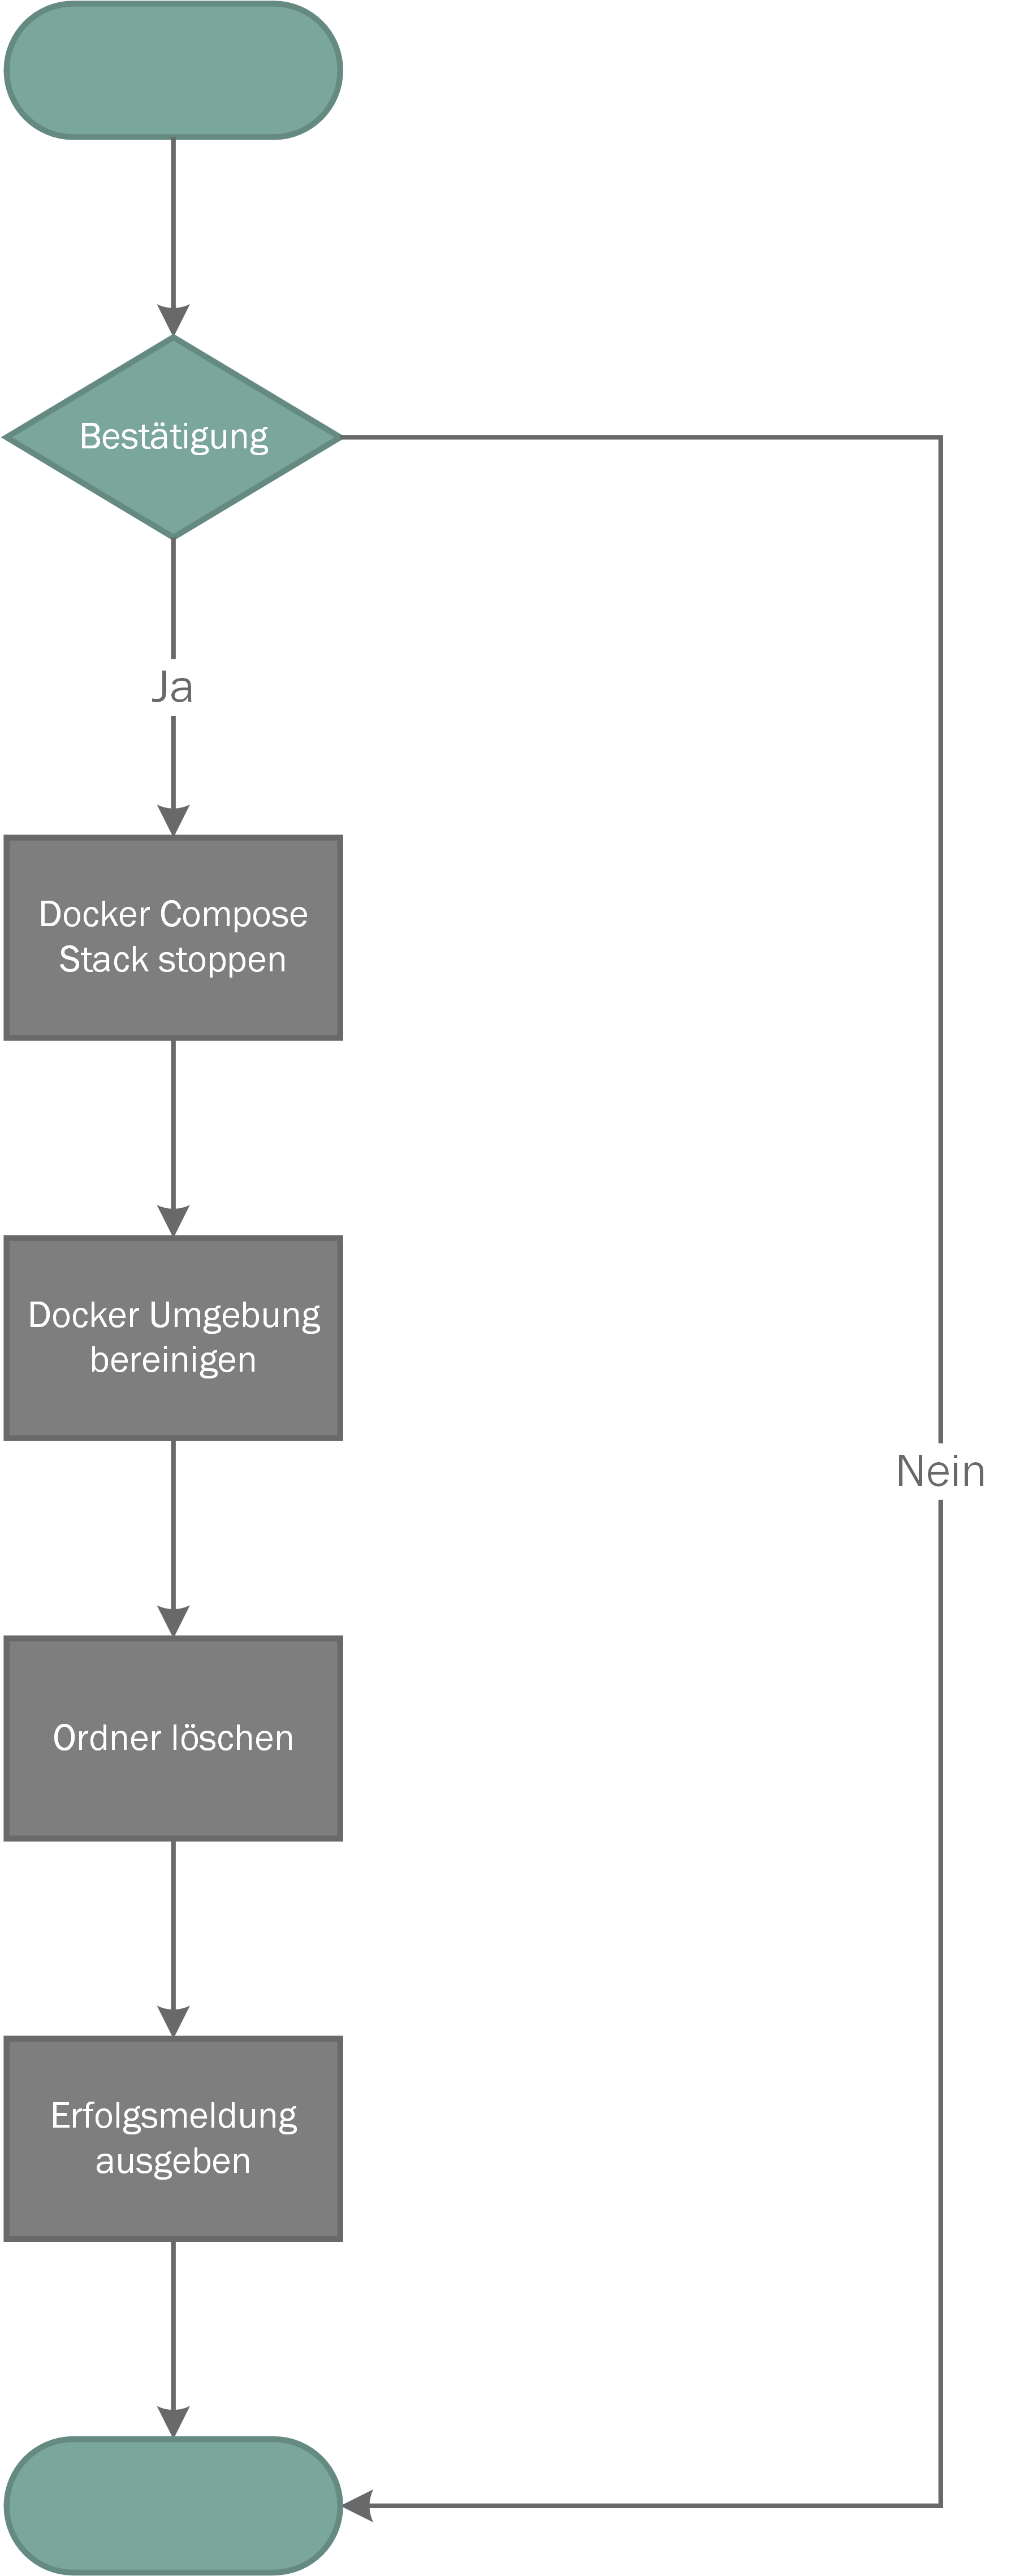
\includegraphics[width=0.48\linewidth]{images/mbeier_konzept/Purge}
	\caption[Flussdiagramm über die Deinstallation]{Flussdiagramm über die Deinstallation}
	\label{fig:purge}
\end{figure}
~\\
Der Vorgang hinter der Deinstallation löscht jegliche Information der Software aus der Docker Umgebung und auch alle Dateien, welche mit den Diensten assoziiert sind.

\newpage

\subsection{Datenmodell}

Auf Basis der zu erstellenden Anträge und der allgemeinen Nutzerverwaltung wurde folgendes Datenmodell entwickelt. Darin wurde speziell darauf geachtet, dass jegliche Information auch wirklich dort zu finden ist, wo sie auch auf einem papieren Antrag zu finden wäre. 

\begin{figure}[H]
	\centering
	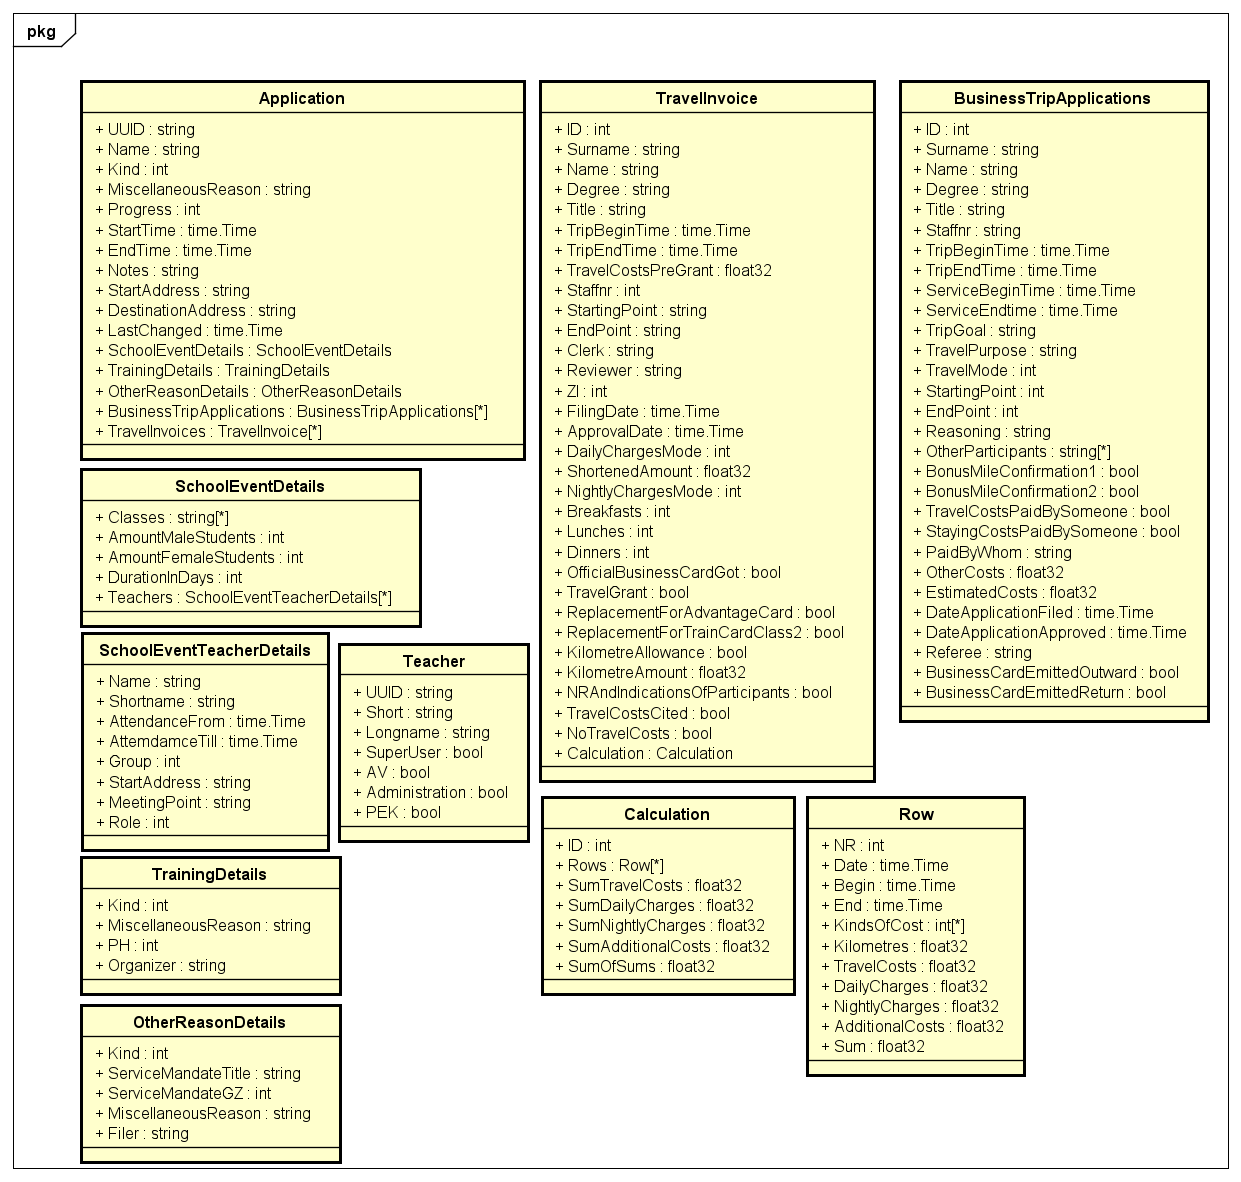
\includegraphics[width=\linewidth]{images/mbeier_konzept/Datamodel}
	\caption[Zentrales Datenmodell]{Das zentrale Datenmodell beinhaltet jegliche Daten, die von der Software benötigt werden.}
	\label{fig:datamodel}
\end{figure}

Im Gesamten gibt es zehn verschiedene Datenstrukturen, wobei hierbei neun die eigentlichen Anträge inklusive Subinformationen widerspiegeln und einer die Lehrkraft-Datenstruktur, welche das Schlüsselelement der Nutzerverwaltung darstellt.

\newpage

\subsection{REST-Schnittstelle}

Die REST-Schnittstelle im Backend ist die Kommunikationsschnittstelle mit dem Systemeigenen Frontend. Sie stellt jegliche Daten und generierte Files zur Verfügung und nimmt diverse Eingaben durch Lehrkräfte auf. Um jeweils diese Daten anzunehmen oder zurückzugeben werden sogenannte Endpoints erstellt. Diese sind in sich abgeschlossene Vorgänge, welche sich jeweils immer auf eine Aufgabe beschränken. Im folgenden Kapitel sind alle geplanten Endpoints beschrieben.

\subsubsection{Endpoints}
\label{chapter:endpoints}

Die folgende Tabelle beschreibt die geplanten Endpoints, wobei  sie jeweils mit der Protokollmethode (GET, POST, PUT oder DELETE), dem Pfad zum Endpoint, einer kurzen Beschreibung, Rückgaben, Eingaben und dem Erfordernis eines Tokens beschrieben werden.

\captionof{table}[REST-Endpoints 1]{Übersicht REST-Endpoints: Teil 1}
\label{table:endpoints1}
\begin{table}
	\centering
	\begin{tabular}{|l|l|l|l|l|}
		\hline
		\multicolumn{1}{|c|}{\textbf{Methode}} & \multicolumn{1}{c|}{\textbf{Endpoint}}                                                  & \multicolumn{1}{c|}{\textbf{Beschreibung}}                                                                  & \multicolumn{1}{c|}{\textbf{\begin{tabular}[c]{@{}c@{}}Rückgabe\\ (Erfolg)\end{tabular}}} & \multicolumn{1}{c|}{\textbf{Eingabe}}                                                                          \\ \hline
		
		
		POST                                   & /login                                                                                  & Loggt eine Lehrkraft ein                                                                                    & Tokenpaar                                                                                 & \begin{tabular}[c]{@{}l@{}}Benutzerinformationen\\ (Nutzername Passwort)\end{tabular}                          \\ \hline
		POST                                   & /logout                                                                                 & Loggt eine Lehrkraft aus                                                                                    & Erfolg                                                                                    & \multicolumn{1}{c|}{--}                                                                                        \\ \hline
		GET                                    & /login/refresh                                                                          & Erneuert einen Login                                                                                        & Tokenpaar                                                                                 & Refresh-Token (als Token)                                                                                      \\ \hline
		GET                                    & /getTeacherByShort                                                                      & \begin{tabular}[c]{@{}l@{}}Gibt Informationen zu \\ einer Lehrkraft zurück\end{tabular}                     & Lehrkraft                                                                                 & \begin{tabular}[c]{@{}l@{}}Abkürzung\\ einer  Lehrkraft\end{tabular}                                           \\ \hline
		GET                                    & /getTeacher                                                                             & \begin{tabular}[c]{@{}l@{}}Gibt Informationen zu\\ einer Lehrkraft zurück\end{tabular}                      & Lehrkraft                                                                                 & UUID einer Lehrkraft                                                                                           \\ \hline
		GET                                    & \begin{tabular}[c]{@{}l@{}}/setTeacher\\ Permissions\end{tabular}                       & \begin{tabular}[c]{@{}l@{}}Setzt die Berechtigungen\\ einer Lehrkraft\end{tabular}                          & Erfolg                                                                                    & \begin{tabular}[c]{@{}l@{}}Lehrkraft-\\ Berechtigungen\end{tabular}                                            \\ \hline
		GET                                    & \begin{tabular}[c]{@{}l@{}}/getActive\\ Applications\end{tabular}                       & \begin{tabular}[c]{@{}l@{}}Gibt alle aktiven Anträge\\ (einer Lehrkraft) zurück\end{tabular}                & \begin{tabular}[c]{@{}l@{}}Liste an\\ Anträgen\end{tabular}                               & \begin{tabular}[c]{@{}l@{}}optional: Name einer\\ Lehrkraft\end{tabular}                                       \\ \hline
		GET                                    & /getAllApplications                                                                     & Gibt alle Anträge zurück                                                                                    & \begin{tabular}[c]{@{}l@{}}Liste an\\ Anträgen\end{tabular}                               & \begin{tabular}[c]{@{}l@{}}optional: Name einer\\ Lehrkraft\end{tabular}                                       \\ \hline
		GET                                    & /getNews                                                                                & \begin{tabular}[c]{@{}l@{}}Gibt die letzt veränderten\\ Anträge zurück\end{tabular}                         & \begin{tabular}[c]{@{}l@{}}Liste an\\ Anträgen\end{tabular}                               & \multicolumn{1}{c|}{--}                                                                                        \\ \hline
		GET                                    & \begin{tabular}[c]{@{}l@{}}/getAdmin\\ Application\end{tabular}                         & \begin{tabular}[c]{@{}l@{}}Gibt alle Anträge zurück,\\ die von einem Admin \\ anzuschauen sind\end{tabular} & \begin{tabular}[c]{@{}l@{}}Liste an\\ Anträgen\end{tabular}                               & \multicolumn{1}{c|}{--}                                                                                        \\ \hline
		
	\end{tabular}
\end{table}	

\newpage
		
\captionof{table}[REST-Endpoints 2]{Übersicht REST-Endpoints: Teil 2}	
\label{table:endpoints2}
\begin{table}
	\centering
	\begin{tabular}{|l|l|l|l|l|}
		\hline
		\multicolumn{1}{|c|}{\textbf{Methode}} & \multicolumn{1}{c|}{\textbf{Endpoint}}                                                  & \multicolumn{1}{c|}{\textbf{Beschreibung}}                                                                  & \multicolumn{1}{c|}{\textbf{\begin{tabular}[c]{@{}c@{}}Rückgabe\\ (Erfolg)\end{tabular}}} & \multicolumn{1}{c|}{\textbf{Eingabe}}                                                                          \\ \hline
		
		GET                                    & /getApplication                                                                         & \begin{tabular}[c]{@{}l@{}}Gibt Informationen zu\\ einem Antrag zurück\end{tabular}                         & Antrag                                                                                    & UUID des Antrages                                                                                              \\ \hline
		POST                                   & /createApplication                                                                      & Erstellt einen Antrag                                                                                       & Erfolg                                                                                    & Antragsdaten                                                                                                   \\ \hline
		PUT                                    & /updateApplication                                                                      & Aktualisiert einen Antrag                                                                                   & Erfolg                                                                                    & Antragsdaten                                                                                                   \\ \hline
		DELETE                                 & /deleteApplication                                                                      & Löscht einen Antrag                                                                                         & Erfolg                                                                                    & Antragsdaten                                                                                                   \\ \hline
		GET                                    & \begin{tabular}[c]{@{}l@{}}/getAbsenceForm\\ ForClasses\end{tabular}                    & \begin{tabular}[c]{@{}l@{}}Erstellt das Abwesenheits-\\ formular von Klassen\end{tabular}                   & PDF                                                                                       & \begin{tabular}[c]{@{}l@{}}UUID des Antrages, \\ optional: Liste an Klassen\end{tabular}                       \\ \hline
		GET                                    & \begin{tabular}[c]{@{}l@{}}/getAbsenceForm\\ ForTeacher\end{tabular}                    & \begin{tabular}[c]{@{}l@{}}Erstellt das Abwesenheits-\\ formular einer Lehrkraft\end{tabular}               & PDF                                                                                       & \begin{tabular}[c]{@{}l@{}}UUID des Antrages, \\ Name der Lehrkraft\end{tabular}                               \\ \hline
		GET                                    & \begin{tabular}[c]{@{}l@{}}/getCompensation\\ ForEducational\\ SupportForm\end{tabular} & \begin{tabular}[c]{@{}l@{}}Erstellt das Formular\\ für pädagogische Betreuung\end{tabular}                  & PDF                                                                                       & UUID des Antrages                                                                                              \\ \hline
		GET                                    & \begin{tabular}[c]{@{}l@{}}/getTravel\\ InvoiceForm\end{tabular}                        & \begin{tabular}[c]{@{}l@{}}Erstellt ein \\ Reiserechnungsformular\end{tabular}                              & PDF                                                                                       & \begin{tabular}[c]{@{}l@{}}UUID des Antrages, \\ Name der Lehrkraft, \\ ID der Reiserechnung\end{tabular}      \\ \hline
		GET                                    & \begin{tabular}[c]{@{}l@{}}/getBusinessTrip\\ ApplicationForm\end{tabular}              & \begin{tabular}[c]{@{}l@{}}Erstellt ein \\ Dienstantragsformular\end{tabular}                               & PDF                                                                                       & \begin{tabular}[c]{@{}l@{}}UUID des Antrages, \\ Name der Lehrkraft, \\ ID des Dienstreiseantrags\end{tabular} \\ \hline
		GET                                    & \begin{tabular}[c]{@{}l@{}}/getTravel\\ InvoiceExcel\end{tabular}                       & \begin{tabular}[c]{@{}l@{}}Erstellt eine Reiserechnung\\ als Excel-Datei\end{tabular}                       & Excel                                                                                     & \begin{tabular}[c]{@{}l@{}}UUID des Antrages, \\ Name der Lehrkraft, \\ ID der Reiserechnung\end{tabular}      \\ \hline
		GET                                    & \begin{tabular}[c]{@{}l@{}}/getBusinessTrip\\ ApplicationExcel\end{tabular}             & \begin{tabular}[c]{@{}l@{}}Erstellt einen Dienstantrag\\ als Excel-Datei\end{tabular}                       & Excel                                                                                     & \begin{tabular}[c]{@{}l@{}}UUID des Antrages, \\ Name der Lehrkraft, \\ ID des Dienstreiseantrags\end{tabular} \\ \hline
		POST                                   & /saveBillingReceipt                                                                     & \begin{tabular}[c]{@{}l@{}}Speichert einen \\ Beleg als PDF ab\end{tabular}                                 & \multicolumn{1}{c|}{--}                                                                   & PDF                                                                                                            \\ \hline
	\end{tabular}
\end{table}

\newpage

\subsubsection{Token System}

Die Implementierung eines nicht-persistenten Token Systems, um die Kommunikation mit der REST-Schnittstelle weiter zu schützen, ist gerade, wenn es sich um sensible Daten handelt sehr wichtig. Ansonsten könnte jeder einfach die Endpoints der Schnittstelle ansprechen. Durch die Ausgabe von sogenannten \enquote{Access Tokens} und \enquote{Refresh Tokens} werden diese jedoch abgesichert. Dies geschieht dadurch, dass diese bei jeder Anfrage nach dem Login mit übergeben werden müssen (im Headerfeld \enquote{Authorization}), wodurch sich der Absender als eingeloggte Lehrkraft verifiziert. Anfragen ohne Tokens werden in Folge automatisch abgewiesen. 
\\Diese Tokens sind verschlüsselte Zeichenketten, welche nur durch das Backend entschlüsselbar sind, da nur das System selbst den Schlüssel hierfür kennt. Im Token selbst werden Informationen über die Sitzung und den Nutzer gespeichert, sodass er nur durch die Angabe des Tokens verifiziert werden kann.\\
Das \enquote{Access Token} ist genau 15 Minuten lang gültig und erlaubt solange direkten Zugriff auf die Schnittstelle. Sobald dieses abgelaufen ist, kann mit dem \enquote{Refresh Token}, welches 7 Tage lang gültig ist, ein neues Tokenpaar bei der Schnittstelle generiert werden. Da es sich um zwei komplett neue Tokens handelt, verlängert sich auch die Gültigkeit des Logins hierbei. Sollte keines der beiden Token mehr gültig sein, so muss ein neues Paar durch einen neuen Loginvorgang erstellt werden.

\subsection{Backend}
Um jene in  \autoref{chapter:endpoints} beschriebenen Endpoints auch mit Funktionalität ausstatten zu können, müssen entsprechende Methoden im Backend implementiert werden. Hierzu gehören hauptsächlich die Schnittstellen zu folgenden Diensten und die Implementierungen von Hauptfunktionen des Systems. Diese sind in den folgenden Abschnitten beschrieben.

\subsubsection{Untis}

Die offizielle Untis-Schnittstelle ermöglicht dem System die Abfrage des aktuellen Stunden- und Supplierplans. Dadurch können diese Informationen auch auf den etwaigen Formularen direkt genutzt werden. Um mit dieser Schnittstelle einfach kommunizieren zu können, ist folgender Aufbau und Implementierung eines REST-Clients im Backend geplant. Mit Hilfe diesen kann das System einfach die Sitzung, welche schon durch die REST-Schnittstelle existiert, weiter nutzen und somit möglichst effizient arbeiten.

\begin{figure}[H]
	\centering
	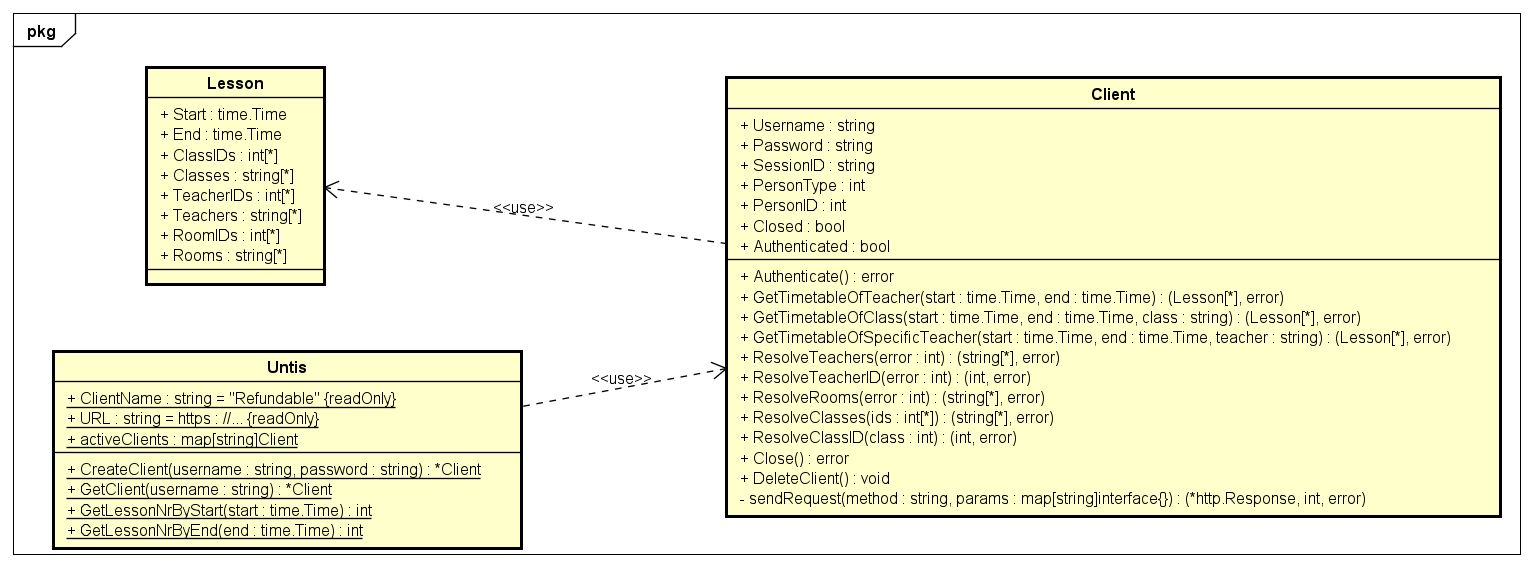
\includegraphics[width=\linewidth]{images/mbeier_konzept/Untis}
	\caption[Untis API-Client UML-Klassendiagramm]{UML-Klassendiagramm des Untis API-Client für das Abfragen von Stundenplaninformationen.}
	\label{fig:untis}
\end{figure}

\newpage

\subsubsection{LDAP}

LDAP ist ein Zugriffsprotokoll um auf ein Active Directory zugreifen zu können. In diesem wird im tgm weitere Informationen zu den Lehrkräften und Schülern gespeichert. Um diese Daten einsehen zu können, muss man sich bei diesem Dienst anmelden, was mit den jeweils eigenen tgm-Account Zugangsdaten möglich ist. Dadurch ist die Anmeldung mit den tgm-Nutzerdaten zu realisieren. Des Weiteren ist die Abfrage weiterer benötigter Daten hierdurch möglich. Der Ablauf einer solchen Interaktion über LDAP wird in folgendem Flussdiagramm veranschaulicht.

\begin{figure}[H]
	\centering
	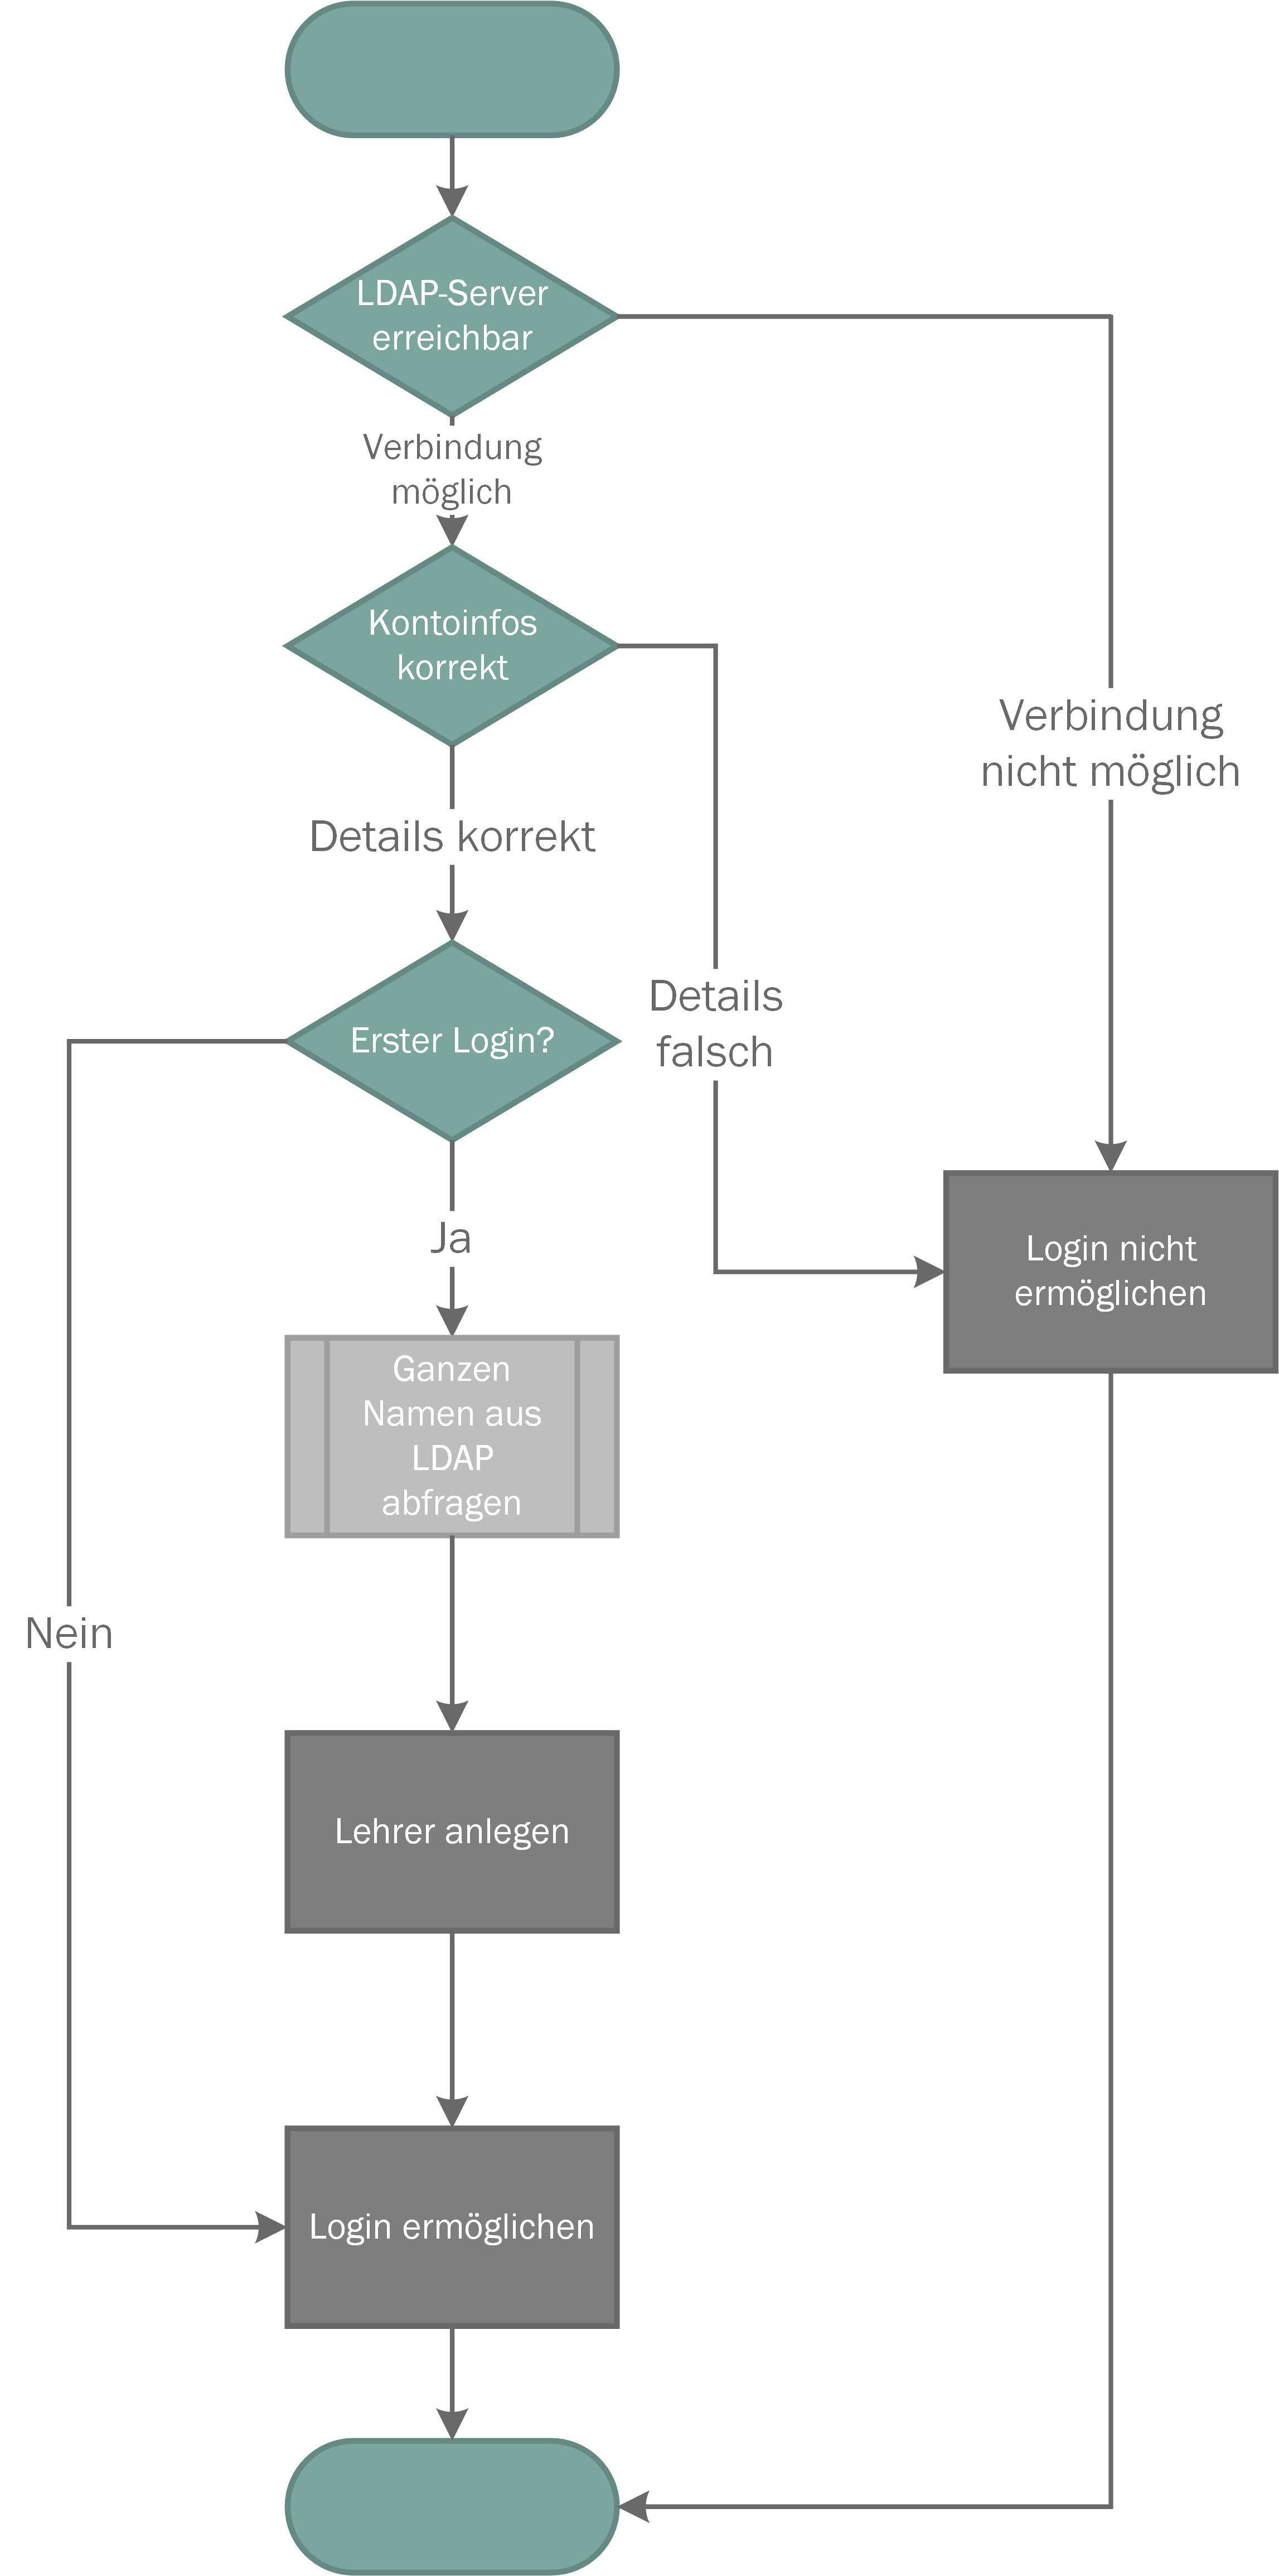
\includegraphics[width=0.5\linewidth]{images/mbeier_konzept/LDAP_Authenticate}
	\caption[Authentifizierung über LDAP]{Authentifizierung über den tgm-eigenen LDAP Server}
	\label{fig:ldapauthenticate}
\end{figure}

\newpage

Um jenen in \autoref{fig:ldapauthenticate} abgebildeten Ablauf einfach implementieren zu können, bietet sich folgender Aufbau eines LDAP-Clients an. Dieser kann dann hierbei die Zugangsdaten durch eine einfache Anmeldung beim Dienst verifizieren und auch die benötigten Daten, den kompletten Namen der Lehrkraft, beim Dienst abfragen.

\begin{figure}[H]
	\centering
	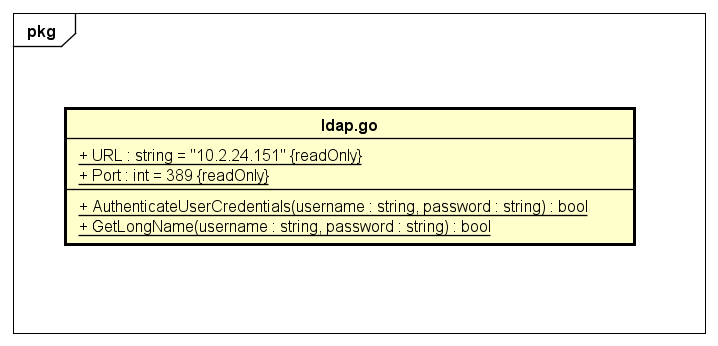
\includegraphics[width=\linewidth]{images/mbeier_konzept/LDAP}
	\caption[lLDAP UML-Klassendiagramm]{UML-Klassendiagramm des LDAP Packages für die Authentifizierung von Lehrkräften}
	\label{fig:ldap}
\end{figure}

\newpage

\subsubsection{Dateierstellung}

Die Datei- und Formularerstellung ist die Hauptfunktion der Software. Das Generieren folgender Forms wird unterstützt. Bei \enquote{Reiserechnung} und \enquote{Dienstreiseantrag} werden auf Grund des festgelegten Designs auch eine Excel Variante angeboten, in der dieses umgesetzt ist. Das Format steht hierbei für Hoch- oder Querformat, wobei Portrait das Hochformat und Landscape das Querformat ist.

\captionof{table}[Dateierstellung - Dateien]{Übersicht über die verschiedenen Dateien, die durch das Backend erstellt werden.}	
\label{tbl:files}
\begin{table}
	\centering
	\begin{tabular}{|l|l|l|}
		\hline
		\multicolumn{1}{|c|}{\textbf{Formular}} & \multicolumn{1}{c|}{\textbf{Dateityp}} & \multicolumn{1}{c|}{\textbf{Format}} \\ \hline
		Abwesenheitsmeldung eines Jahrganges & PDF & Portrait \\ \hline
		Abwesenheitsmeldung eines Lehrers & PDF & Portrait \\ \hline
		Abgeltung für pädagogische Betreuung & PDF & Portrait \\ \hline
		Reiserechnung & PDF & Landscape \\ \hline
		Dienstreiseantrag & PDF & Portrait \\ \hline
		Reiserechnung & Excel & Landscape \\ \hline
		Dienstreiseantrag & Excel & Portrait \\ \hline
	\end{tabular}
\end{table}

~\\
Alle eigens generierten PDFs sind jedenfalls mit einer Kopfzeile ausgestattet. In dieser ist in der linken Ecke das tgm-Logo zu sehen, in der Mitte steht der Name des Formulars (siehe \autoref{tbl:files}) und rechts ein QR-Code, welcher einen nach dem Scan auf die Website führt und den zugehörigen Antrag dort direkt öffnet.

\begin{figure}[H]
	\centering
	
\includegraphics[width=\linewidth]{images/mbeier_konzept/Kopfleiste_PDF_border}
	\caption[Kopfleiste PDF-Datei]{Beispiel einer Kopfleiste in den vom Backend generierten PDF-Dateien}
	\label{fig:kopfleiste-pdf}
\end{figure}


\lfoot{Ryan Foster}
%!TEX root=../../main.tex
\section{Datenschnittstelle und Webseitenlogik}
Die Schnittstelle zwischen Frontend und Backend wird mittels eines JavaScript-Frameworks umgesetzt. Wie in Kapitel \hyperref[sec:rfoster_fazit]{5.3.5} beschrieben, wird hierfür VueJS verwendet. VueJS bietet viele passende Funktionen und Features um solch eine Webseite umzusetzen.
\subsection{Webseitenlogik}
\label{sec:webseitenlogik}
Die Webseite wird mittels Vue-Komponenten aufgebaut werden. Eine Seite besteht aus einer Hauptkomponente und möglicherweise noch zusätzliche Nebenkomponenten. Die Struktur der einzelnen Komponenten und Links der Webseite wird wie folgt aussehen:
\begin{figure}[H]
	\centering
	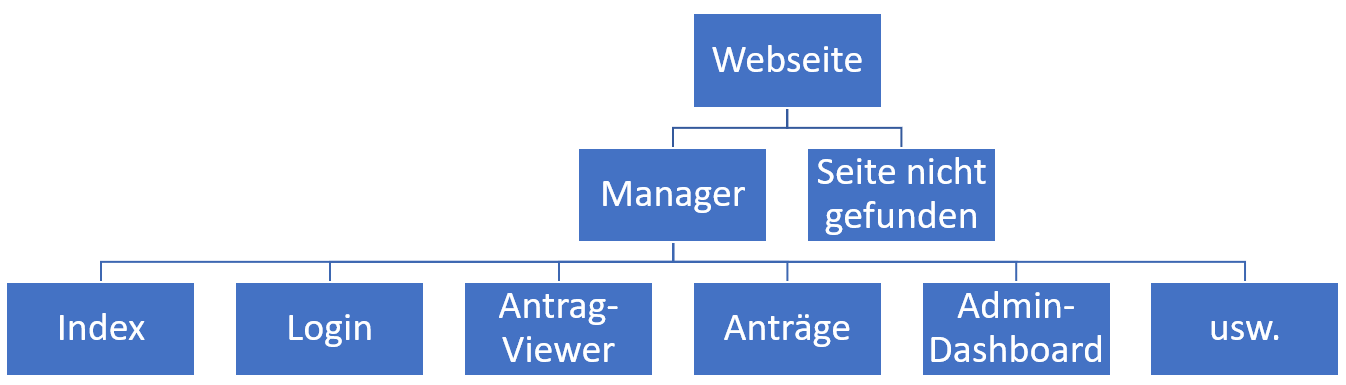
\includegraphics[width=0.8\linewidth]{images/Webseite_hierarchie}
	\caption[Hierarchie der Webseite]{Übersicht der Hierarchie der Webseite}
	\label{fig:webseitehierachie}
\end{figure}

\subsubsection{Seite nicht gefunden}
Wird ein Link eingegeben werden, welcher nicht die Seite selbst oder eine definierte Unterseite ist, wird eine Seite geladen, bei der der Benutzer darauf hingewiesen wird, dass er keinen korrekten Link eingegeben hat.
\begin{figure}[H]
	\centering
	
\includegraphics[width=0.6\linewidth]{images/page_not_found}
	\caption[Seite nicht gefunden]{Seite nicht gefunden}
	\label{fig:pagenotfound}
\end{figure}

\subsubsection{Manager}
Der Manager ist der Hauptbestandteil der Webseite. Er beinhaltet alle einzelnen Seiten und zeigt immer die gewünschten Seite an. In dem Manager werden auch Cookie-Einstellungen und Rechte gespeichert. Fast alle Komponenten werden dem Manager untergeordnet sein. Der Manager ist auch dafür verantwortlich zwischen Komponenten Daten zu senden.

\subsubsection{Komponenten}
Einzelne Komponenten laden die Daten eigenständig aus dem Backend. Dies ist eine Maßnahme, um den Manager nicht mit Funktionen zu überladen und damit nicht Daten bei jedem Aufruf von dem Manager an die einzelnen Komponenten gesendet werden müssen.\\
Im Falle, dass eine Komponente Daten an eine weitere Komponente sendet, wird diese Kommunikation von dem Manager übernommen.

\subsubsection{Antrag-Viewer}
Es wird eine weitere Seite vorhanden sein, auf die man durch einen Link gelangen kann. Auf dieser Seite ist es möglich, einen Antrag per ID anzeigen zu lassen. Da dieser extra Link technisch auf der selben Ebene, wie der Manager ist, wird dafür gesorgt, dass dieser extra Link dem Manager nahtlos untergeordnet ist. Der Antrag-Viewer ist nur verwendbar, sofern der Benutzer angemeldet ist und auch die Berechtigung hat diesen Antrag zu betrachten.
\\\\
Wird in den Parametern des Links bereits spezifiziert, welcher Antrag geöffnet werden soll, wird nach der Anmeldung dem Benutzer dieser Antrag angezeigt. Es können nur jene Anträge angezeigt werden, zu denen der Benutzer die erforderlichen Berechtigungen besitzt. Besitzt der Benutzer nicht die erforderlichen Berechtigungen, wird eine Fehlermeldung ausgegeben.

\subsubsection{Navigation}
Da fast alle Komponenten dem Manager untergeordnet sind, ist es auch die Verantwortung des Managers die Navigation zu steuern. Dazu gibt es eine zentrale Funktion im Manager, welche die derzeit geladene Seite verändern kann. Des Weiteren werden die benötigten Informationen geladen bzw. erstellt, welche die Komponenten benötigen.
\\\\
Die Funktion zum Verändern der derzeitigen Anzeige, wird von den untergeordneten Komponenten aufgerufen. Hinzu kommt, dass mit dem Aufruf der Funktion auch spezifiziert wird, welche Seite geladen werden soll. Spezielle Seiten, wie z.B: der Antrag-Viewer benötigen zusätzlichen Informationen, welche über diese Funktion mitgegeben werden.

\subsubsection{Features}
Es werden auch Funktionen implementiert, welche das Benützen der Webseite erleichtern.
\\\\
Es ist möglich bei erneutem Laden der Webseite auf die zuletzt geöffnete Seite zu gelangen. Bei Beenden des Browsers speichert die Webseite die aktuelle Seite und lädt diese bei erneutem Aufrufen der Webseite.
\\\\
Es ist auch möglich zwischen den Seiten durch die Browser-Pfeile zu navigieren. Dies ist wichtig, da durch versehentliches Drücken einer falschen Komponente ein Benutzer möglichst schnell wieder auf die vorherige Seite gelangen können muss. Durch die Implementierung der Browser-Pfeile ist es möglich intuitiv auf die vorherige Seite zu wechseln. Andere Funktionen, welche die selben Funktionalität haben, werden durch diese Implementierung auch unterstützt.
\newpage
\subsection{Daten laden}
Auf den Seiten, bei denen es benötigt wird, werden über Funktionen des Frameworks dynamisch Komponenten erstellt und geladen. Der Prozess um Daten aus dem Backend zu laden wird in folgender Grafik beschrieben:
\begin{figure}[H]
	\centering
	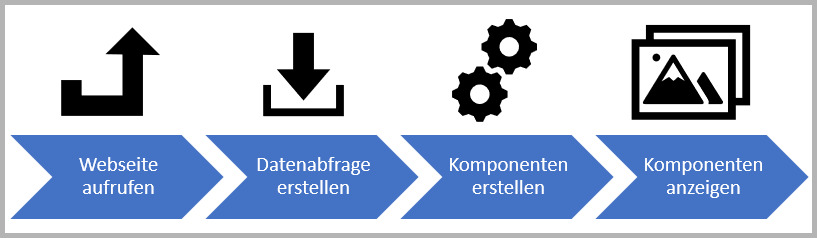
\includegraphics[width=0.8\linewidth]{images/Prozess_Daten_laden}
	\caption[Prozess der Daten zur Anzeige]{Übersicht über den Prozess, welcher Daten aus dem Backend lädt}
	\label{fig:prozessdatenladen}
\end{figure}

\subsubsection{Webseite aufrufen}
Die Webseite wird aufgerufen und der Benutzer bekommt die Startseite angezeigt.

\subsubsection{Datenabfrage erstellen und Daten erhalten}
Auf der Startseite der Webseite werden die neuesten Nachrichten angezeigt, welche für den Lehrer relevant sind. Hierfür müssen aus dem Backend Daten geladen werden. Dies erfolgt über eine Abfrage, welche aus dem Frontend gesendet wird. Diese werden ausgelesen und verwendet um Komponenten zu erstellen.

\subsubsection{Komponenten erstellen}
Die geladenen Daten aus dem Backend werden mittels Einbindung der Variablen in einzelne Komponenten eingebunden.\\
Seiten, auf denen viele gleiche Komponenten sind, werden mittels Schleifen erstellt. Diese sorgen dafür, dass nicht zu viele Komponenten auf der Seite geladen sind, wenn diese nicht gebraucht werden.
Ein Beispiel hierfür sind die neuen Nachrichten, welche in folgender Grafik gezeigt werden:
\begin{figure}[H]
	\centering
	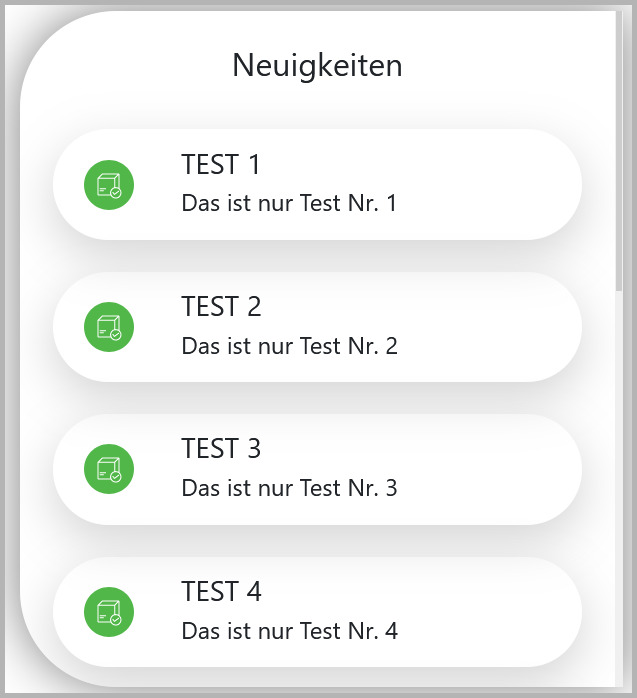
\includegraphics[width=0.3\linewidth]{images/messages_index}
	\caption[Neue Nachrichten]{Grafik der neuen Nachrichten}
	\label{fig:messagesindex}
\end{figure}

\subsubsection{Komponenten anzeigen}
Die bereits erstellten Komponenten werden über die Einbindung in der Webseite angezeigt. Dies kann durch einfache Implementierung bei einzelnen Komponenten sein.\\
Durch die Schleife, können auch die Komponenten angezeigt werden. Diese ordnet alle Komponenten hintereinander an und zeigt diese an.\\
Bei den Nachrichten kann man sich jede Nachricht als eigene Komponente vorstellen, welche jeweils erstellt und danach angezeigt wird.
%\newpage
\subsection{Befehle senden}
Die Webseite besitzt auch einige Aktionen, die von Benutzern ausgeführt werden können. Diese müssen je nach Aktion eine neue Seite aufrufen oder einen Befehl an das Backend senden.

\begin{figure}[H]
	\centering
	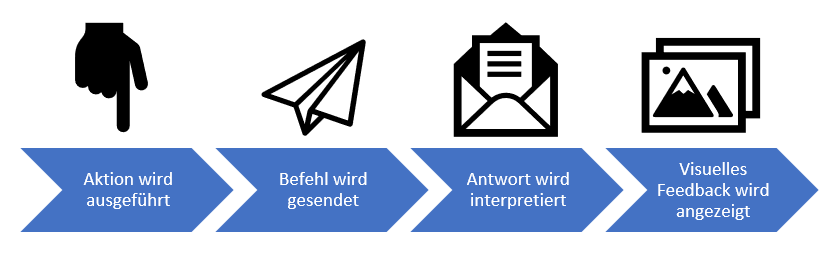
\includegraphics[width=0.8\linewidth]{images/Prozess_Befehl_senden}
	\caption[Prozess der Befehlssendung]{Übersicht über den Prozess welcher Befehle an das Backend sendet}
	\label{fig:prozessbefehlsenden}
\end{figure}

\subsubsection{Aktion ausführen}
Eine Aktion wird ausgeführt, wenn z.B: auf eine Komponente gedrückt wird. Dies ruft eine Funktion auf, bei der ein Befehl erstellt wird.

\subsubsection{Befehl senden}
Der Befehl beinhaltet alle wichtigen Informationen für das Backend. Beispielsweise, falls eine neue Nachricht gelöscht werden soll, wird die ID der Nachricht mitgesendet.

\subsubsection{Antwort interpretieren}
Sobald das Backend den Befehl ausgeführt hat, wird eine Antwort an das Frontend gesendet und wird dort interpretiert. Die Interpretation der Antwort wird durch den Status der Antwort geschehen. Der Status der Antwort beinhaltet einen Code, welcher aussagt, ob der Befehl funktioniert hat oder fehlgeschlagen ist. Sollte der Befehl fehlgeschlagen sein, so deutet der Code auf den genauen Fehlergrund hin.

\subsubsection{Information anzeigen}
Tritt ein Fehler auf, wird dem Benutzer dies offensichtlich mitgeteilt werden.\\
Sollte kein Fehler aufgetreten sein, soll dem Benutzer je nach Befehl dies auf unterschiedliche Weise mitgeteilt werden.\\
Um weiterhin das Beispiel zu nutzen: Wenn eine Nachricht gelöscht werden soll, dann wird dem Benutzer mitgeteilt, dass die Nachricht gelöscht worden ist, wenn diese Nachricht verschwindet.
\lfoot{Linus Dehner, Michael Beier, Ryan Foster}
%!TEX root=../main.tex
\chapter{Implementierung}
Hier wird die Umsetzung des Projekts beschrieben und auf Details zu den einzelnen Technologien eingegangen. Im Optimalfall werden die Lösungen und Wege zu den zuvor definierten Problemen und Zielen geschildert. Eine bestehende Dokumentation, welche während der Arbeit erstellt wurde kann hier von großem Vorteil sein!
\lfoot{Linus Dehner}
%!TEX root=../../main.tex
\section{Frontend}
In diesem Kapitel wird die Erstellung eines Konzepts für das Frontend erläutert. Dabei müssen Faktoren wie beispielsweise unsere Zielgruppe, die Lehrerschaft beachtet werden. Im folgenden Kapitel werden die theoretischen Hintergründe des Konzeptes überlegt, danach werden erste Entwürfe mittels Mockups erstellt. 
\subsection{Vorbereitung}
Wie im Kapitel 5.1 und 5.3 festgelegt wird im Frontend Bootstrap in Verbindung mit VueJS verwendet. Zu aller erst muss daher VueJS auf dem Computer, auf dem das Projekt erstellt wird, installiert werden. Dies geschieht auf Windows über den Node Packet Manager (NPM) \cite{vue-install}. Der Befehl um VueJS zu installieren schaut wie folgt aus:
\begin{code}{bash}
	npm install -g @vue/cli
\end{code}
Nachdem VueJS installiert ist kann man in das gewünschte Verzeichnis wechseln und über
\begin{code}{bash}
	vue create refundable
\end{code}
ein neues Vue Projekt erstellen, das in diesem Fall \enquote{Refundable} heißt \cite{vue-create-project}. Um die Funktionalität von Bootstrap und VueJS optimal auszunutzen wird Bootstrap direkt mit dem Node Packet Manager zu VueJS installiert \cite{bootstrap-vue-getting-started}:
\begin{code}{bash}
	npm install vue bootstrap-vue
\end{code}
Damit ist die Arbeit aber noch nicht getan, um in den Komponenten Bootstrap und dessen vordefinierte Icons zu verwenden, muss man in \enquote{main.js} folgendes importieren:
\begin{code}{html}
	import { BootstrapVue, BootstrapVueIcons } from "bootstrap-vue";
	import "./plugins/bootstrap-vue";
	
	Vue.use(BootstrapVue);
	Vue.use(BootstrapVueIcons);
\end{code}
\captionof{listing}{Benötigte Befehle um Bootstrap im VueJS Projekt einzubinden}
	\label{list:requcommands} ~\\
Alle Teile der Website sind in sogenannten Komponenten verpackt, die je nach Benutzereingaben dynamisch gewechselt werden. 

\newpage
\subsection{Komponenten der Website}
\subsubsection{Generell}
Die Struktur der Komponenten ist so aufgebaut, dass die Seite sowohl für Desktop- als auch mobile Endgeräte optimiert ist. Dazu wird das \enquote{Grid-System} von Bootstrap verwendet, welches seinen Platz im \enquote{template-Tag}, der VueJS Komponente findet. Dieses besteht aus einem Container, einer Reihe (Row) und einer Spalte (Column). Da es am Anfang das Problem gab, dass nicht der ganze Bildschirm ausgenutzt wurde, habe ich folgende Klassen in unserem CSS-Dokument erstellt:
\begin{code}{css}
	.template-main-container {
		height: 100vh;
		width: 100vw;
		margin: 0;
		padding: 0;
	}
	
	.template-main-row {
		height: 100vh;
		width: 100vw;
		margin: 0;
		padding: 0;
	}
\end{code}
\captionof{listing}{CSS Klassen für die Haupt- Contianer und Reihen}
	\label{list:cssmaincont} ~\\
Diese dienen dazu, dass der Hauptcontainer, als auch die Hauptreihe der Website, 100\% der Höhe (100 vertikale Einheiten), sowie 100\% der Breite (100 horizontale Einheiten) einnehmen. Außerdem wird in den Klassen definiert, dass die Elemente keinen Abstand zum Rand haben sollen.
\newpage
\subsubsection{Login-Seite}
Uns war sehr wichtig, dass die Login-Seite sehr schlicht gehalten ist und sofort zu verstehen ist. Da das Tool Refundable nur von Lehrern des TGMs verwendet werden soll, haben wir uns dazu entschlossen, dass in der Loginmaske die E-Mail-Endung \enquote{@tgm.ac.at} vordefiniert und unveränderbar ist. Außerdem wollten wir dem Aufrufer der Website sofort klar machen, um was es sich bei dieser Website handelt und haben daher den Projektnamen Refundable, als auch unseren Slogan auf der Seite platziert. Des weiteren war aufgrund der DSGVO eine Meldung zu realisieren, die den Benutzer darüber informiert, dass Cookies verwendet werden. Falls diese Meldung nicht akzeptiert wird und man versucht sich anzumelden, wird eine Fehlermeldung dargestellt. Diese Meldung wird jedoch dynamisch mit VueJS erstellt und nicht direkt mittels Bootstrap. In der Realität schaut die Login-Seite wie folgt aus (Abbildung 7.1):
\begin{figure}[H]
	\centering
	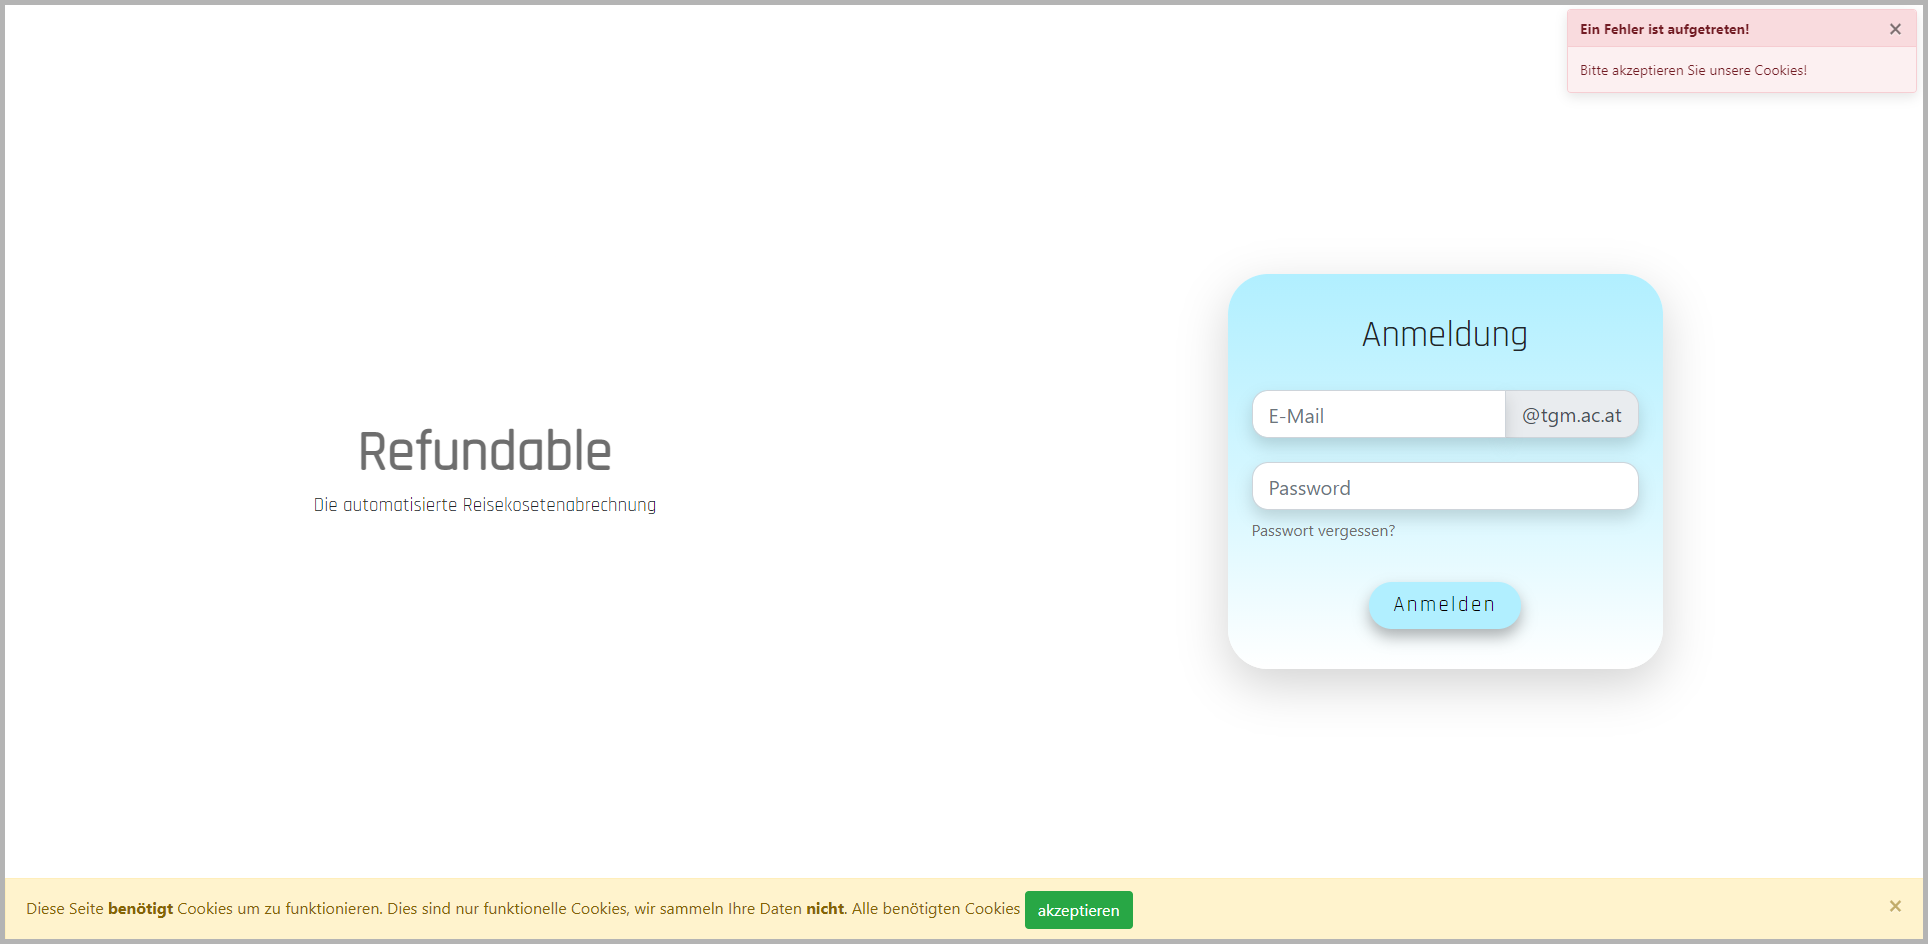
\includegraphics[width=1\linewidth]{images/website/login}
	\caption[Login]{Ein Bild der endgültigen Login-Seite}
	\label{fig:login}
\end{figure}
\paragraph{Login-Maske}
~\\
Die Login-Maske besteht aus einem eigenen Container, welcher ermöglicht die Maske vollkommen responsiv aufzubauen. Die Eingabefelder haben wir mit einer \enquote{input-groupe} gelößt (Code Z. 12). Um einen Wert optisch in einem Eingabefeld vorzugeben hat Bootstrap ein praktisches Element, namens \enquote{b-input-groupe-text} (Code Z. 14), welches vor oder nach dem Feld hinzugefügt werden kann. Da die Login-Daten, der TGM Server verwendet werden, haben wir einen Link eingebaut, falls man sein Passwort vergessen hat. Betätigt man diesen, wird man auf die entsprechende Seite des TGMs weitergeleitet.
\begin{code}{html}
	<!-- Anmeldungsformular -->
	<b-col cols="12" md="6">
		<b-container>
			<b-row align-h="center">
				<b-col cols="12" sm="10" md="10" lg="8" xl="6">
					<b-container id="login-wrap" class="shadow-lg">
						<b-row id="r-login" align-h="center">
							<h2 id="lheading2">Anmeldung</h2>
						</b-row>
						<b-row align-h="center" id="r-email">
							<b-col cols="12">
								<!-- Input des Benutzernamens / der Email -->
								<b-input-group size="lg">
									<b-input-group-text
										id="tgm-addon"
										class="shadow"
										slot="append"
										><span>@tgm.ac.at</span></b-input-group-text
										>
									<b-form-input
										id="email"
										class="shadow login-inputs"
										v-model="email"
										type="text"
										placeholder="E-Mail"
									></b-form-input>
								</b-input-group>
							</b-col>
						</b-row>
						<b-row id="r-password">
							<b-col cols="12">
								<!-- Input des Passworts -->
								<b-form-input
									id="password"
									class="shadow login-inputs"
									v-model="password"
									type="password"
									placeholder="Password"
									size="lg"
								></b-form-input>
							</b-col>
						</b-row>
						<b-row id="r-forgotten">
							<b-col cols="12">
								<!-- Passwort vergessen Weiterleitung auf Moodle -->
								<a
									id="forgotten-password"
									href="https://elearning.tgm.ac.at/login/forgot_password.php"
								>Passwort vergessen?</a
								>
							</b-col>
						</b-row>
						<b-row align-h="center" id="r-login-btn">
							<!-- Login Button -->
							<b-button size="lg" id="login-btn" v-on:click="login"
							>Anmelden</b-button
							>
						</b-row>
					</b-container>
				</b-col>
			</b-row>
		</b-container>
	</b-col>
\end{code}
\captionof{listing}{HTML Code der Login-Maske}
	\label{list:loginmask} ~\\
Da einige Elemente unseren Ansprüchen optisch nicht genügt haben, haben wir eigene Änderungen in unserem CSS-Code hinzugefügt. Dabei wurde vor allem die Gestaltung, der Eingabefelder und des Buttons verändert, aber auch die des Containers, welcher die Maske beinhaltet. Genauer gesagt haben wir den Farbverlauf des Logos in der Maske eingebaut, die Ecken der Elemente etwas abgerundet und Schatten hinzugefügt.
\begin{code}{css}
/* -- Login -- */

#login-wrap {
	background: rgb(255, 255, 255);
	background: -moz-linear-gradient(
	0deg,
	rgba(255, 255, 255, 1) 0%,
	rgba(220, 248, 255, 1) 38%,
	rgba(177, 239, 255, 1) 100%
	);
	background: -webkit-linear-gradient(
	0deg,
	rgba(255, 255, 255, 1) 0%,
	rgba(220, 248, 255, 1) 38%,
	rgba(177, 239, 255, 1) 100%
	);
	background: linear-gradient(
	0deg,
	rgba(255, 255, 255, 1) 0%,
	rgba(220, 248, 255, 1) 38%,
	rgba(177, 239, 255, 1) 100%
	);
	filter: progid: DXImageTransform.Microsoft.gradient(startColorstr="#ffffff", endColorstr="#b1efff", GradientType=1);
	padding: 1.5rem;
	border-radius: 2.5rem;
}

#email {
	border-radius: 1rem 0 0 1rem;
}

#tgm-addon {
	border-radius: 0 1rem 1rem 0;
}

.input-group-append {
	border-radius: 0 1rem 1rem 0;
}

.input-group-text {
	border-radius: 0 1rem 1rem 0;
}

#password {
	border-radius: 1rem 1rem 1rem 1rem;
}

#login-btn {
	font-family: "Rajdhani", sans-serif;
	padding: 0.5rem 1.5rem 0.5rem 1.5rem;
	font-size: 1.3rem;
	letter-spacing: 2.5px;
	font-weight: 500;
	color: #000;
	background-color: rgba(177, 239, 255, 1);
	border: none;
	border-radius: 45px;
	box-shadow: 0px 8px 15px rgba(0, 0, 0, 0.3);
	transition: all 0.3s ease 0s;
	cursor: pointer;
	outline: none;
}

#login-btn:hover {
	background-color: #2ec0e5;
	box-shadow: 0px 15px 20px rgba(46, 229, 157, 0);
	color: #fff;
	transform: translateY(3px);
}
\end{code}
\captionof{listing}{CSS Code der Login-Maske}
	\label{list:csslogin} ~\\
\paragraph{Cookie-Meldung}
~\\
Die Meldung, dass Cookies benutzt werden, sollte schlicht und einfach sein. Außerdem haben wir uns als Ziel gesetzt, dass sie dem Nutzer deutlich klar machen soll, dass wir ausschließlich funktionelle und notwendige Cookies verwenden. Für diese Meldung hat sich perfekt das vordefinierte \enquote{Alert-Element} von Bootstrap geeignet:
\makeatletter
\begin{code}{html}
	<!-- Bestätigung, dass diese Seite Cookies benutzt -->
	<b-alert
		v-model="showBottom"
		class="position-fixed fixed-bottom m-0 rounded-0"
		style="z-index: 2000;"
		variant="warning"
		dismissible
	>
		Diese Seite <b>benötigt</b> Cookies um zu funktionieren. Dies sind nur
		funktionelle Cookies, wir sammeln Ihre Daten <b>nicht</b>. Alle benötigten
		Cookies
		<!-- Button zum akzeptieren -->
		<b-button variant="success" @click="validateCookies()"
			>akzeptieren
		</b-button>
	</b-alert>
\end{code}
\makeatother
\captionof{listing}{HTML Code Cookie akzeptieren }
	\label{list:cookiehtml} ~\\
\newpage
\subsubsection{Startseite}
Die Startseite sollte so intuitiv und übersichtlich wie möglich sein. Deswegen haben wir uns für ein \enquote{Drei Spalten Design} entschieden. In der ersten Spalte befinden sich alle wichtigen Funktionen - drei Knöpfe, zum erstellen von neuen Anträgen, um alle aktiven Anträge anzuschauen und um alle Anträge zu betrachten, die man jemals gestellt hat. In der 2. Spalte befindet sich das Logo, eine Illustration für das Dashboard und ein Knopf zum Ausloggen. Falls man ein Administrator ist, wird hier ebenfalls ein Knopf, zum wechseln in die Administratoransicht angezeigt. In der dritten Spalte werden Neuigkeiten zu den Anträgen des Benutzers angezeigt, falls man auf eine Neuigkeit klickt, wird man zu dem jeweiligen Antrag weitergeleitet. In der Realität schaut die Startseite wie folgt aus (Abbildung 7.2):
\begin{figure}[H]
	\centering
	
\includegraphics[width=1\linewidth]{images/website/dashboard}
	\caption[Dashboard]{Ein Bild der endgültigen Startseite}
	\label{fig:dashboard}
\end{figure}
Jedoch ist dieses System auf mobilen Geräten nicht sonderlich übersichtlich, deshalb haben wir diese etwas abgeändert. Diese ist sehr schlicht gehalten, jedoch macht dies das Ganze auf Smartphones um einiges einfacher die Website zu bedienen. Die mobile Version der Startseite schaut in der Realität wie folgt aus (Abbildung 7.3):
\begin{figure}[H]
	\centering
	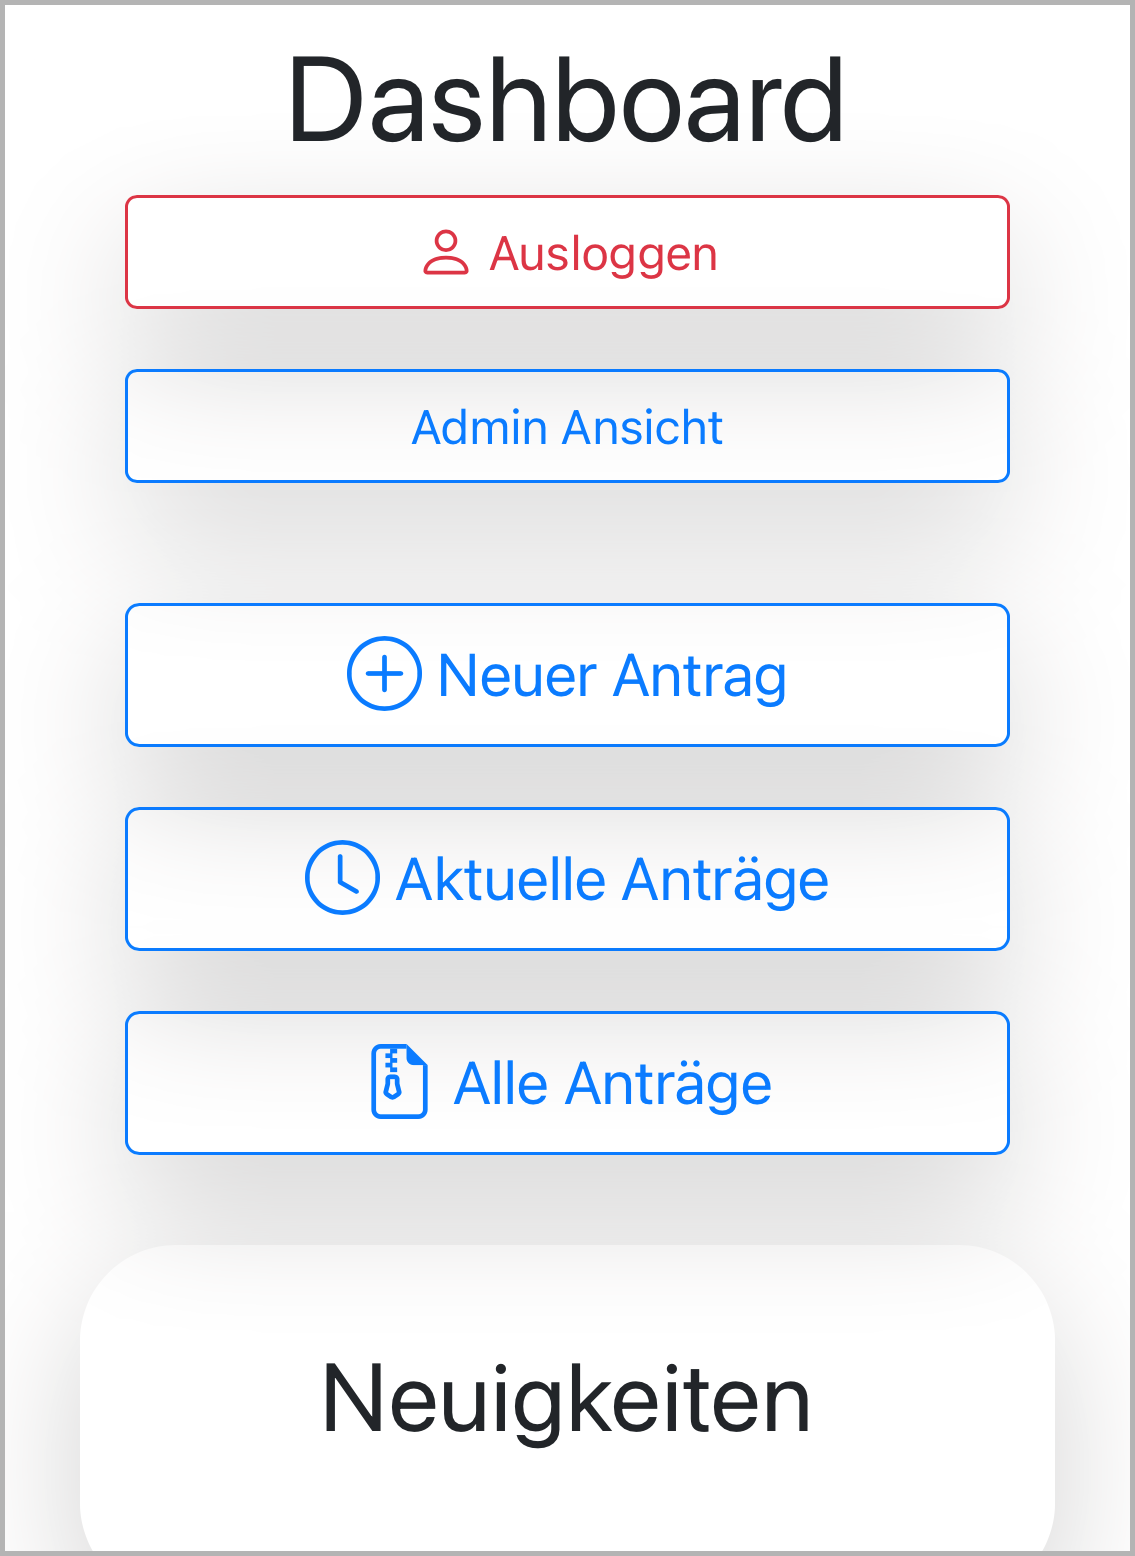
\includegraphics[width=0.4\linewidth]{images/website/dashboard_mobile}
	\caption[Dashboard Mobil]{Ein Bild der endgültigen Startseite (Mobil)}
	\label{fig:dashboardmobile}
\end{figure}

\paragraph{Menü-Element Desktop}
~\\
Der Container mit den Funktionselementen, hat wie beim Login einen Schatten, der ihn von dem Hintergrund abhebt. In diesem Container befinden sich die Menü Bezeichnung und die klickbaren Elemente, die auch aus einem Container bestehen und eine responsive Illustration, die zu der jeweiligen Funktion passt und eine Bezeichnung, was dieser Knopf auslöst beinhaltet.
\begin{code}{html}
<b-col id="dash-main-cont" class="d-none d-md-block" cols="12" md="4">
	<b-container>
		<b-row
			id="dash-row"
			align-v="center"
			align-h="center"
			class="shadow-xl"
		>
			<b-col cols="12">
				<center><h2 id="menu-h2">Menü</h2></center>
			</b-col>
			<!-- Custom Button für einen neuen Antrag -->
			<b-col
				id="new"
				cols="12"
				class="shadow-lg dash-elem"
				v-on:click="newApplication"
			>
				<b-container style="height: 100%">
					<b-row align-h="center" align-v="center" style="height: 100%">
						<b-col cols="6" class="ill-wrapper d-none d-md-block">
						<!-- Illustration neuer Antrag -->
							<b-img
								id="all-ill"
								center
								src="@/assets/new.svg"
								alt="Illustration für alle Anträge"
							></b-img>
						</b-col>
						<b-col cols="12" md="6">
							<h2 id="new-h2" class="dh">Neuer Antrag</h2>
						</b-col>
					</b-row>
				</b-container>
			</b-col>
			
			...
		</b-row>
	</b-container>
</b-col>
\end{code}
\captionof{listing}{HTML-Code-Teile des Startseitenmenüs}
	\label{list:menuhtml} ~\\
Optisch wurde vor allem die Höhe des umschließenden Containers verändert und dessen umliegende Abstände. Wie man auf der Abbildung 7.2 sehen kann wurden hier auch wieder die Ecken abgerundet. Was man jedoch nicht sehen kann, ist, dass sich die Funktionselemente, optisch absenken und der Schatten entfernt und die Farbe verändert wird, wenn man mit der Maus, die sich zu einer zeigenden Hand verändert, über das Element fährt. 
\begin{code}{css}
#dash-main-cont {
	height: 70vh;
}

#dash-row {
	height: 70vh;
	padding-left: 2rem;
	padding-right: 2rem;
	padding-bottom: 1.5rem;
}

.dash-elem {
	background-color: rgb(255, 255, 255);
	height: 22%;
	transition: all 0.3s ease 0s;
	cursor: pointer;
	outline: none;
}

.dash-elem:hover {
	background-color: #8ff2ff;
	box-shadow: 0px 0px 50px rgba(0, 0, 0, 0.144);
	color: rgb(141, 141, 141);
	transform: translateY(3px);
}

#dash-row {
	border-radius: 6rem 6rem 6rem 6rem;
}
\end{code}
\captionof{listing}{Teile des CSS Codes, des Startseitenmenüs}
	\label{list:cssmenu} ~\\
\paragraph{Menü-Element Mobil}
~\\
Wie schon erwähnt ist die mobile Ansicht sehr schlicht gehalten, damit sie nicht überladen wirkt und dass sich auch vor allem die nicht Technik affinen Lehrer auskennen. Daher zeigen wir auf der mobilen Ansicht nur das Nötigste an (Siehe Abbildung 7.3). Alle Knöpfe werden nun vertikal angeordnet und mit einem passenden Icon bestückt. Die Newselemente unterscheiden sich kaum von denen der Desktop-Version, die Elemente sind lediglich mit etwas weniger Details bestückt und sind nicht in einem scrollbaren Container, da man auf der mobilen Version sonst doppelt scrollen müsste.
\begin{code}{html}
	<!-- DASH MOBILE -->
	<b-col class="d-block d-md-none" cols="12">
	  <!-- Column -->
	  <b-container fluid>
		<b-row align-v="center" align-h="center">
		  <b-col cols="12">
			<center><h1 style="margin-top:10px;">Dashboard</h1></center>
		  </b-col>
		  <b-col cols="12">
			<!-- Logout Button -->
			<b-button
			  variant="outline-danger"
			  class="shadow-lg"
			  v-on:click="logout"
			  style="margin-top:0px; margin-bottom:20px; width:100%"
			>
			  <b-icon icon="person" aria-hidden="true"></b-icon> Ausloggen
			  <!-- Icon -->
			</b-button>
		  </b-col>
		  <b-col cols="12">
			<!-- Neuer Antrag Button --><b-button
			  size="lg"
			  variant="outline-primary"
			  v-on:click="newApplication"
			  class="shadow-lg"
			  style="margin-bottom:20px; width:100%"
			>
			  <b-icon icon="plus-circle" aria-hidden="true"></b-icon> Neuer
			  Antrag
			</b-button></b-col
		  >	
\end{code}
\captionof{listing}{Teile des HTML-Codes der mobilen Startseite}
	\label{list:startmobile} ~\\
\paragraph{Neuigkeiten-Element}
~\\
Die Neuigkeiten-Elemente sind mit einer Illustration bestückt, die den momentanen Status des jeweiligen Antrags beschreiben soll. Außerdem wird ein Titel der Neuigkeit mitgegeben, die zum Beispiel \enquote{Antrag X abgelehnt} heißen könnte. Etwas mehr Details werden dann noch in einem Beschreibungsfeld mitgegeben, das wegen der Übersichtlichkeit nur auf Desktopgeräten sichtbar ist.
\begin{code}{html}
	<b-row align-v="center">
	<b-col cols="2">
	  <b-container style="height: 100%">
		<b-row align-v="center" align-h="center" style="height: 100%">
		  <!-- Illustration Angenommen/Abgelehnt -->
		  <img
			src="@/assets/accepted_1.svg"
			class="align-middle news-status"
			style="height: 50px; width: auto"
			alt="Illustration von arbeitenden Personen"
		  />
		</b-row>
	  </b-container>
	</b-col>
	<b-col cols="10">
	  <b-container>
		<b-row align-h="center" align-v="center">
		  <b-col cols="12">
			<!-- Titel der Neuigkeit -->
			<h3 class="news-elem-heading">{{ snews.title }}</h3>
		  </b-col>
		</b-row>
		<b-row align-h="center" class="d-none d-md-block">
		  <b-col cols="12">
			<!-- Beschreibung der Neuigkeit -->
			<h4 class="news-elem-heading">{{ snews.description }}</h4>
		  </b-col>
		</b-row>
	  </b-container>
	</b-col>
  </b-row>	
\end{code}
\captionof{listing}{HTML Code, des Neuigkeiten Elementes}
	\label{list:htmlnews} ~\\
\newpage
\subsubsection{Neuer Antrag}
Auf diese Seite gelangt der Nutzer entweder, durch die Betätigung des \enquote{Neuer Antrag} Buttons auf der Startseite, oder über die Verknüpfung auf der \enquote{Alle Anträge} oder \enquote{Aktive Anträge} Ansicht. Da es nicht möglich ist, ein einheitliches Formular zu kreieren, haben wir uns dazu entschieden, vor dem Formular eine Auswahlmöglichkeit der Antragsart einzubauen.
\paragraph{Auswahl}
~\\
Die von uns gewählte Auswahlmöglichkeit ist sehr einfach und intuitiv gestaltet. Die drei verschiedenen Hauptarten von Anträgen sind klar und deutlich zu unterscheiden. Optisch sind die Knöpfe ähnlich strukturiert, wie die der Hauptseite, damit sich ein einheitliches Design durch die Website zieht.
\begin{figure}[H]
	\centering
	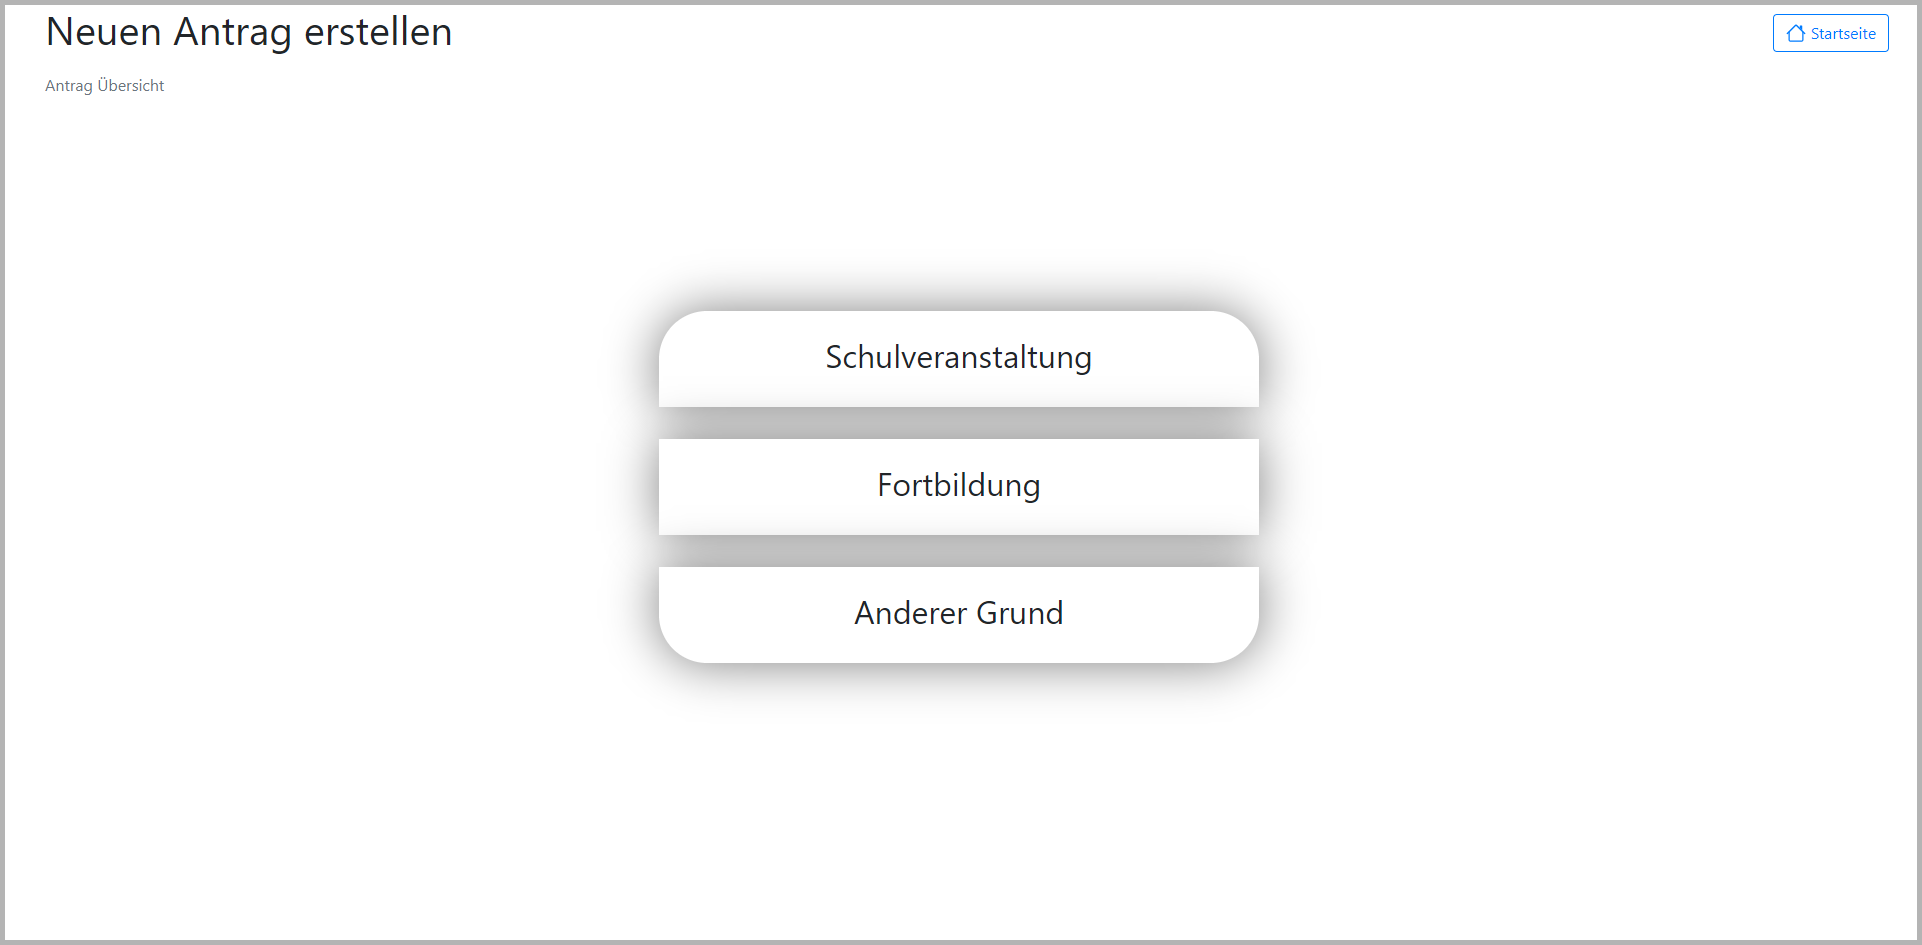
\includegraphics[width=1\linewidth]{images/website/neu}
	\caption[Neuer Antrag Auswahl]{Ein Bild der endgültigen Seite, um ein einen neuen Antrag auszuwählen}
	\label{fig:neuauswahl}
\end{figure}
Die Knöpfe sind wiedermals in eigenen Containern dargestellt, um sie optimal der Größe des Endgerätes anzupassen. In dem Container, der sich mit einem Schatten vom Hintergrund abhebt, ist eine eindeutige Bezeichnung der Funktion, des jeweiligen Elementes. Fährt man mit der Maus über einen Knopf, wird dieser, wie auf der Startseite in seiner Farbe verändert.
\begin{code}{html}
	<b-container id="school-button" class="na-elem shadow-xl">
	<!-- Custom Button zum erstellen eines Schulantrages -->
	<b-row
	  class="na-elem-sr"
	  align-v="center"
	  v-on:click="school()"
	>
	  <b-col cols="12">
		<h2 class="na-elem-h">Schulveranstaltung</h2>
	  </b-col>
	</b-row>
  </b-container>	
\end{code}
\captionof{listing}{HTML Code, einer Auswahlmöglichkeit}
	\label{list:htmlselect} ~\\
\paragraph{Schulveranstaltung}
~\\
Der Antrag für eine neue Schulveranstaltung ist der komplexeste Antrag mit den meisten Eingabefeldern. Außerdem gehören zu dem Antrag für eine Schulveranstaltung auch die Begleitpersonen Anträge. Um die Eingabe von Uhrzeiten und Daten einfacher zu machen, haben wir die Elemente \enquote{b-form-datepicker} und \enquote{b-form-timepicker} verwendet. Dies sind standardmäßige Elemente, die von BootstrapVue vordefiniert sind. Um den Lehrern auf den ersten Blick klar zu machen, welche Daten in welches Feld eingefügt werden, haben wir alle Eingabefelder mit einem Titel und einer Info bestückt.
\begin{figure}[H]
	\centering
	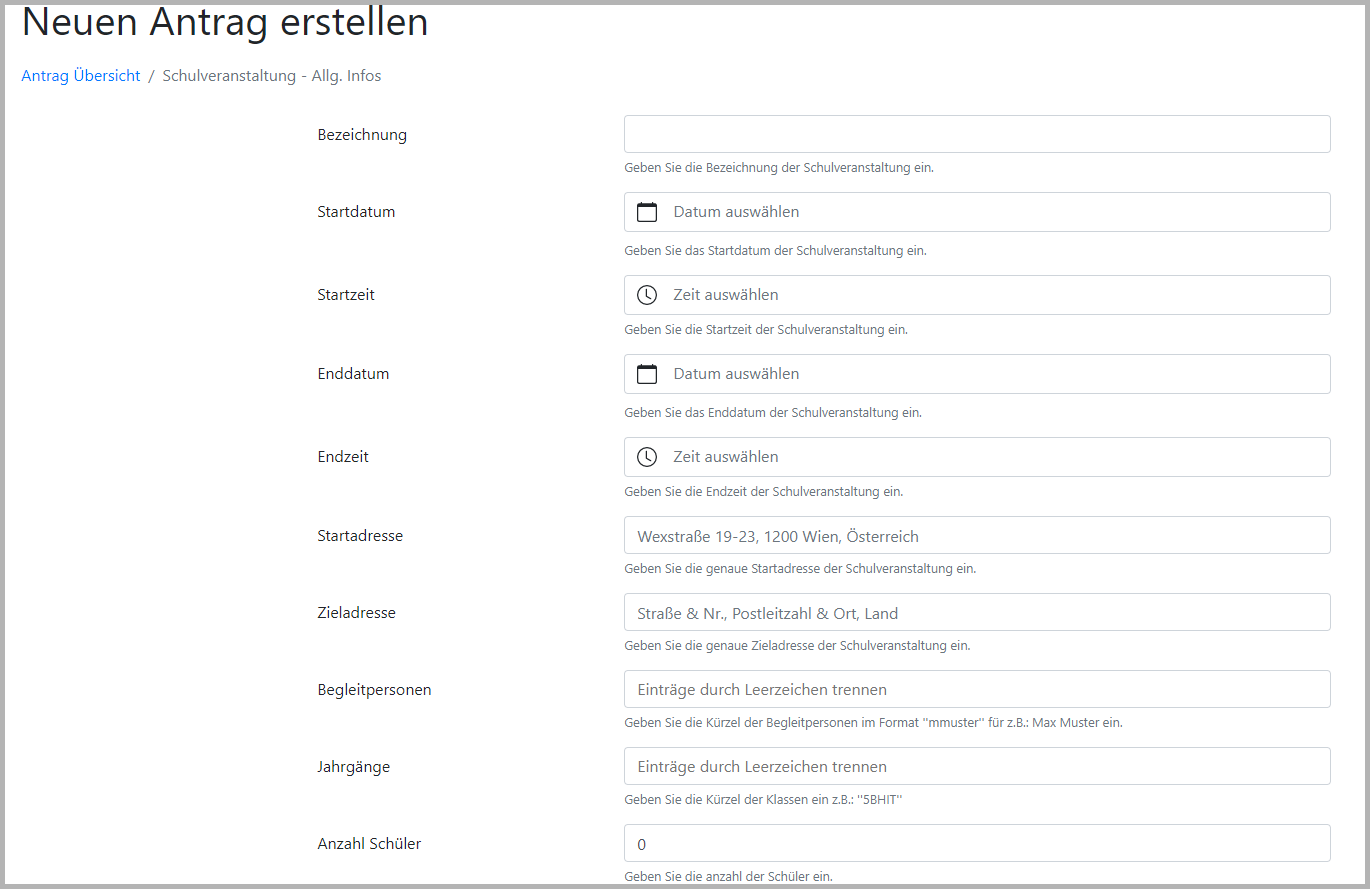
\includegraphics[width=1\linewidth]{images/website/schul_1}
	\caption[Neuer Schulantrag]{Ein Bild der Schulantrags Seite (Teil 1)}
	\label{fig:schulantrag1}
\end{figure}
\begin{figure}[H]
	\centering
	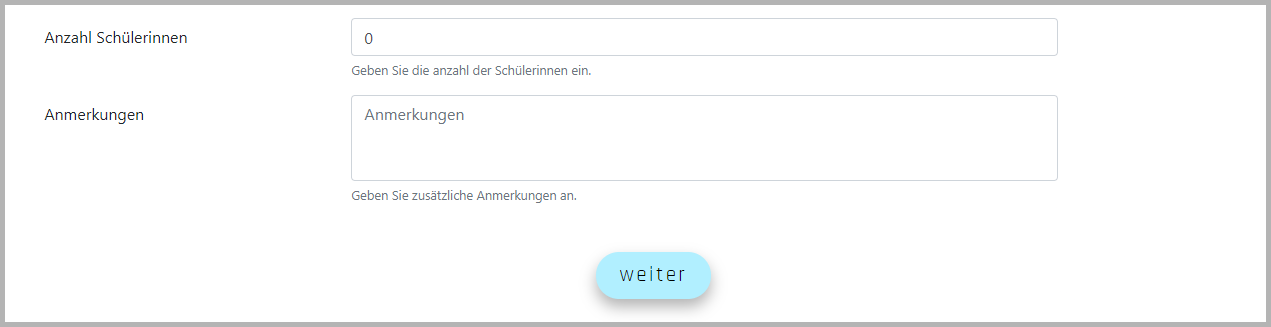
\includegraphics[width=1\linewidth]{images/website/schul_2}
	\caption[Neuer Schulantrag]{Ein Bild der Schulantrags Seite (Teil 2)}
	\label{fig:schulantrag2}
\end{figure}
Alle Eingabefelder sind in sogenannte \enquote{b-form-groups} eingefügt. Diese Elemente bieten die Möglichkeit, einen Titel, der in unserem Fall auf der linken Seite angebracht ist und eine Beschreibung, die unterhalb des Eingabefelds eingefügt ist, hinzuzufügen - natürlich sind diese Elemente auch responsiv. In der \enquote{form-group} wird dann das jeweilige Element eingefügt, welches man eigentlich einbauen will. Diese Elemente können beispielsweise normale Eingabefelder sein, Checkboxe, Radiobuttons, Timepicker, Datepicker, etc.. 
\begin{code}{html}
	<b-form-group
        id="bez"
        label-cols-sm="4"
        label-cols-lg="3"
        content-cols-sm
        content-cols-lg="7"
        description="Geben Sie die Bezeichnung der Schulveranstaltung ein."
        label="Bezeichnung"
        label-for="bezeichnung"
    >
        <b-form-input
            id="bezeichnung"
            v-model="data.Name"
            :readonly="readonly"
            @input="updateData"
        ></b-form-input>
    </b-form-group>
\end{code}
\captionof{listing}{Beispiel für eine Eingabegruppe}
Das Timepicker Element kann ganz einfach, wie im oberen Absatz beschrieben, in eine Eingabegruppe eingefügt werden. Da das Element von Bootstrap vordefiniert ist, muss man leidiglich die üblichen Werte, wie ID und Platzhalter setzen. Das Einzige, das man wirklich beachten muss, ist, dass man die Richtige Zeitzone (Auflistung 7.13 locale) wählt.
\begin{code}{html}
	<b-form-timepicker
		id="stz"
		v-model="startTime"
		:readonly="readonly"
		@input="updateTime"
		locale="de"
		placeholder="Zeit auswählen"
  	></b-form-timepicker>
\end{code}
\captionof{listing}{Timepicker}
Der Datepicker ist noch einfacher zu bedienen, als der Timepicker. Hier sind nur die üblichen Parameter zu setzen.
\begin{code}{html}
	<b-form-datepicker
		id="end"
		v-model="endDate"
		:readonly="readonly"
		@input="updateTime"
		class="mb-2"
		placeholder="Datum auswählen"
  	></b-form-datepicker>
\end{code}
\captionof{listing}{Datepicker}
	\label{list:bspinputgroup} ~\\
Aus den, im Formular angegebenen Daten, wird automatisch ein weiteres Formular generiert. Dies geschieht, nachdem der \enquote{weiter} Button betätigt wurde und alle Daten als Valide anerkannt wurden. Das Formular beinhaltet für jede Begleitperson die geforderten Eingabefelder (Abbildung 7.7). Die Struktur dieser Elemente ist exakt die Selbe, wie die, der Elemente, die in Abbildung 7.11 besprochen wurden. 
\begin{figure}[H]
	\centering
	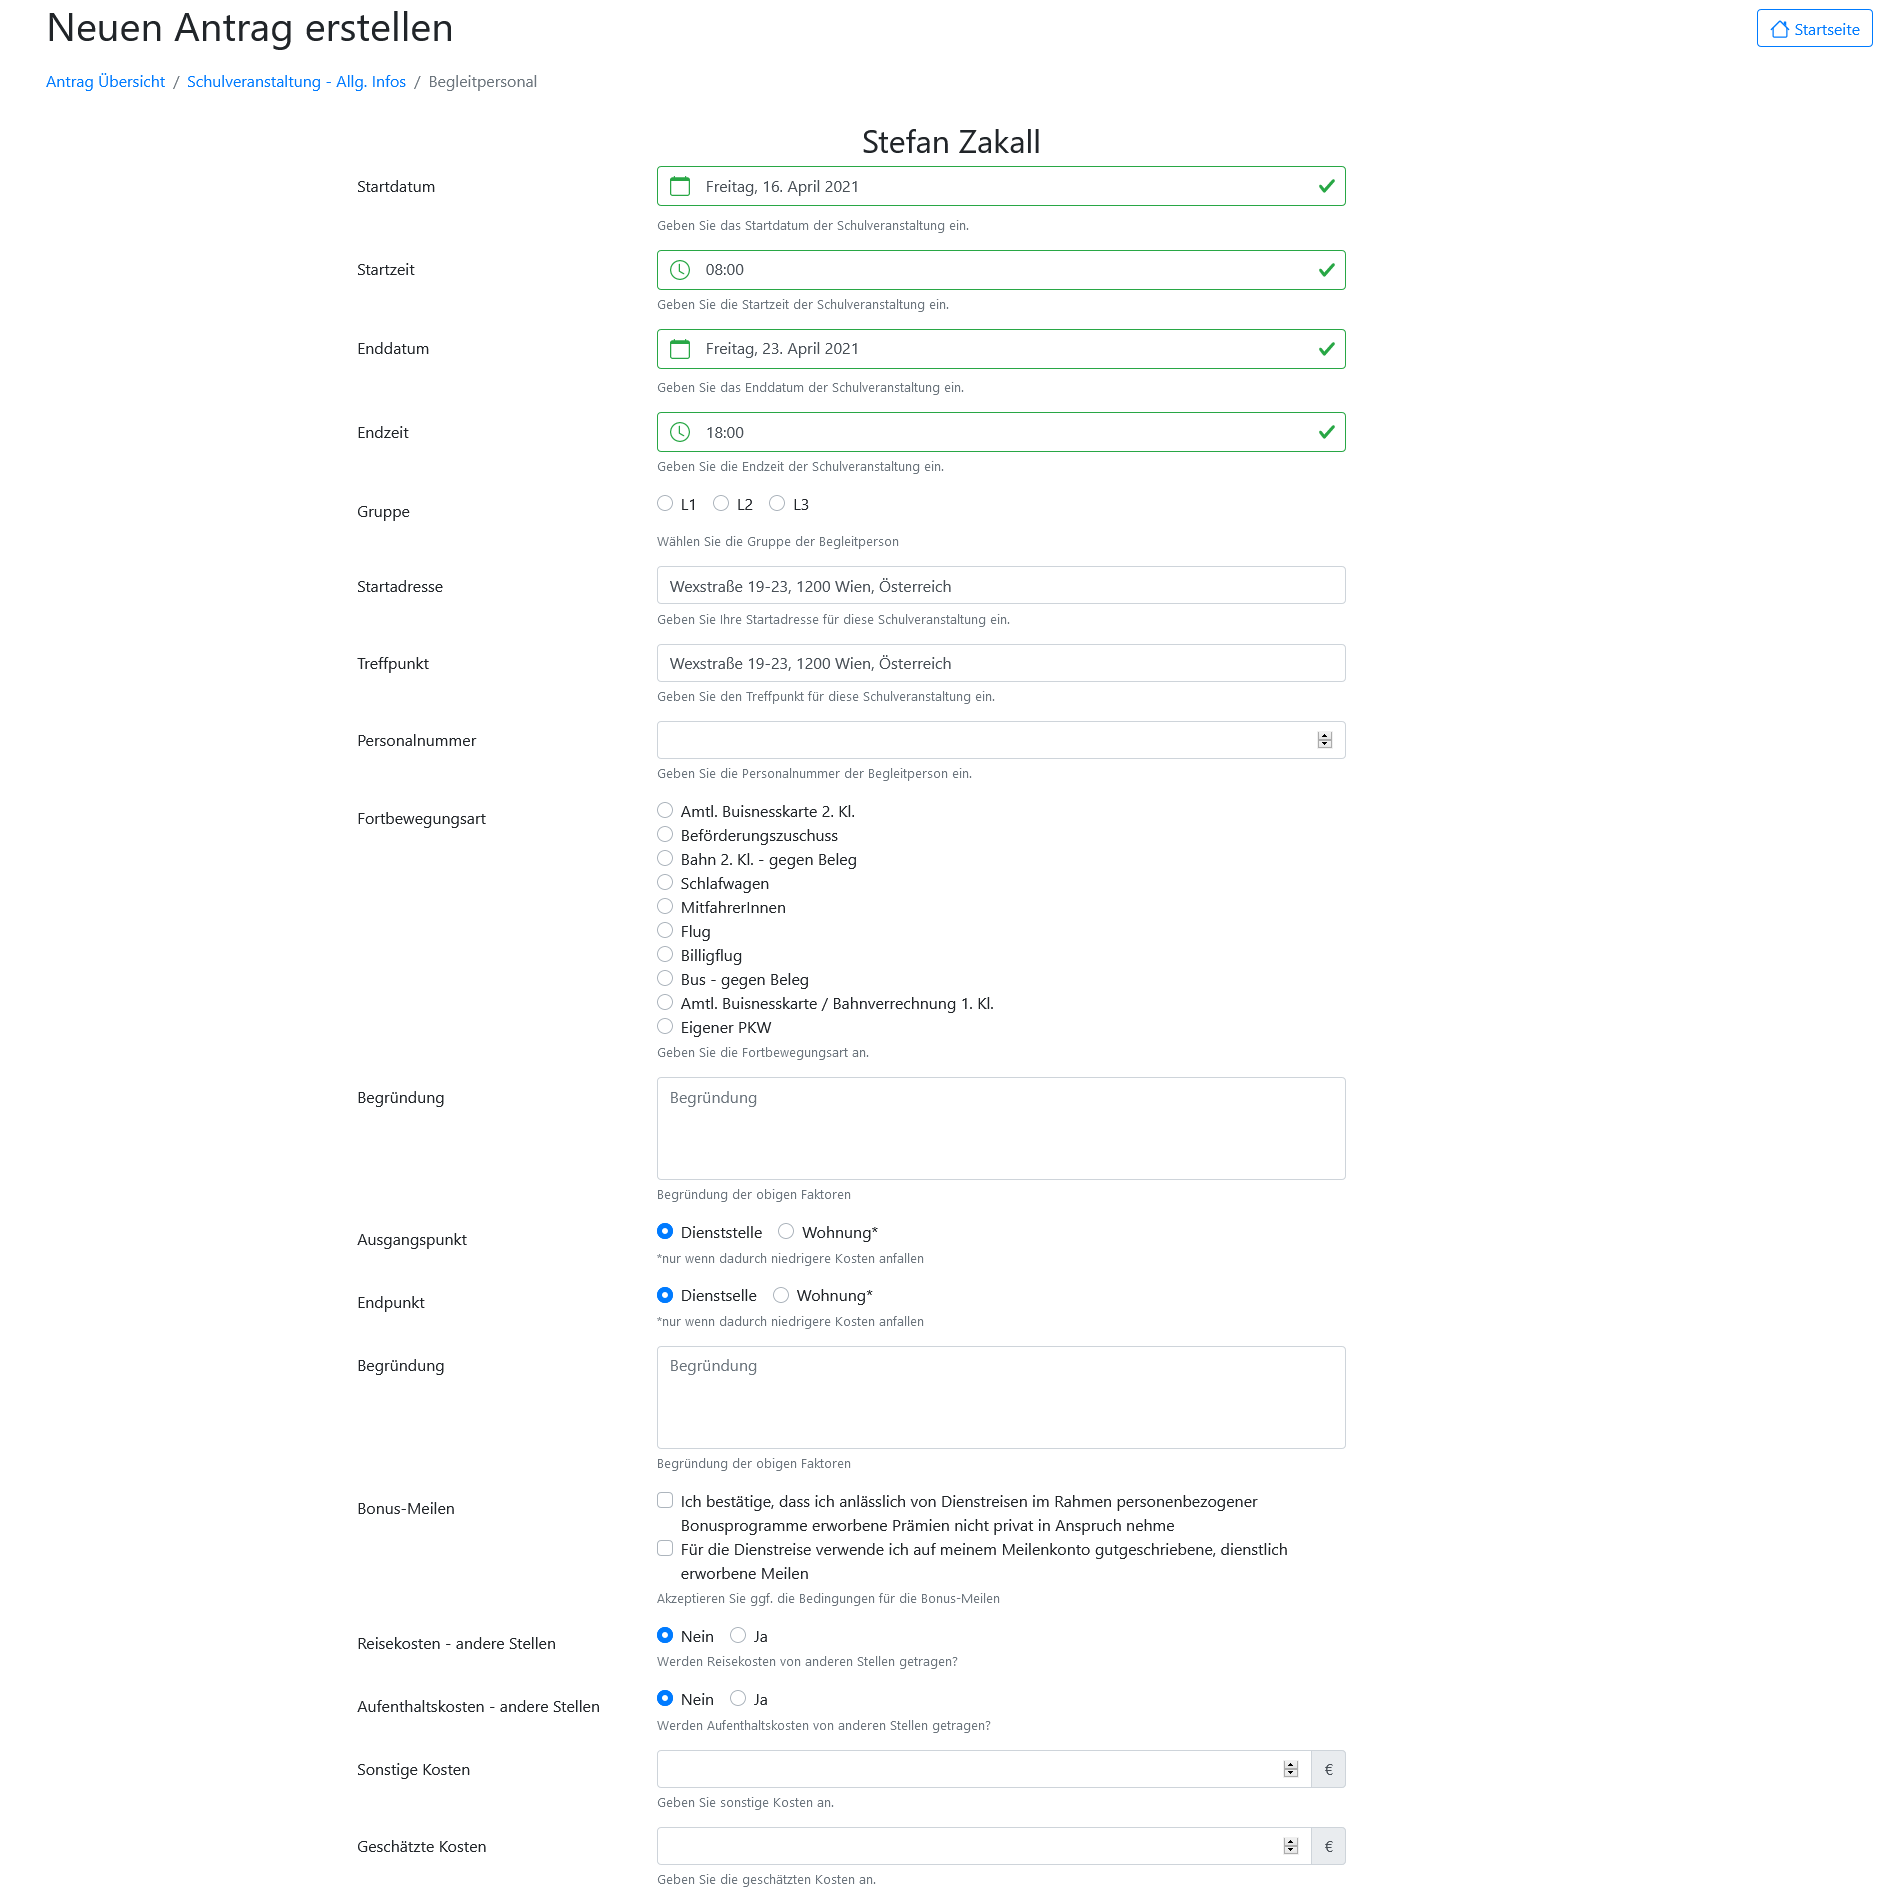
\includegraphics[width=1\linewidth]{images/website/schul_3_1}
	\caption[Neuer Schulantrag]{Ein Bild des Begleitformulars (Teil 1)}
	\label{fig:schulantrag3}
\end{figure}
\paragraph{Fortbildung}
~\\
Das Fortbildungsformular ist für Seminare, Tagungen, Lehrgänge und sonstige Events in dieser Art gedacht. Um die Formulare einheitlich zu halten, wurde auch hier wieder die selbe Struktur der Eingabefelder verwendet. Falls man die sonstige Art auswählt, fügt sich automatisch eine zusätzliche Eingabe hinzu, in der man das Anliegen genauer spezifizieren kann.
\begin{figure}[H]
	\centering
	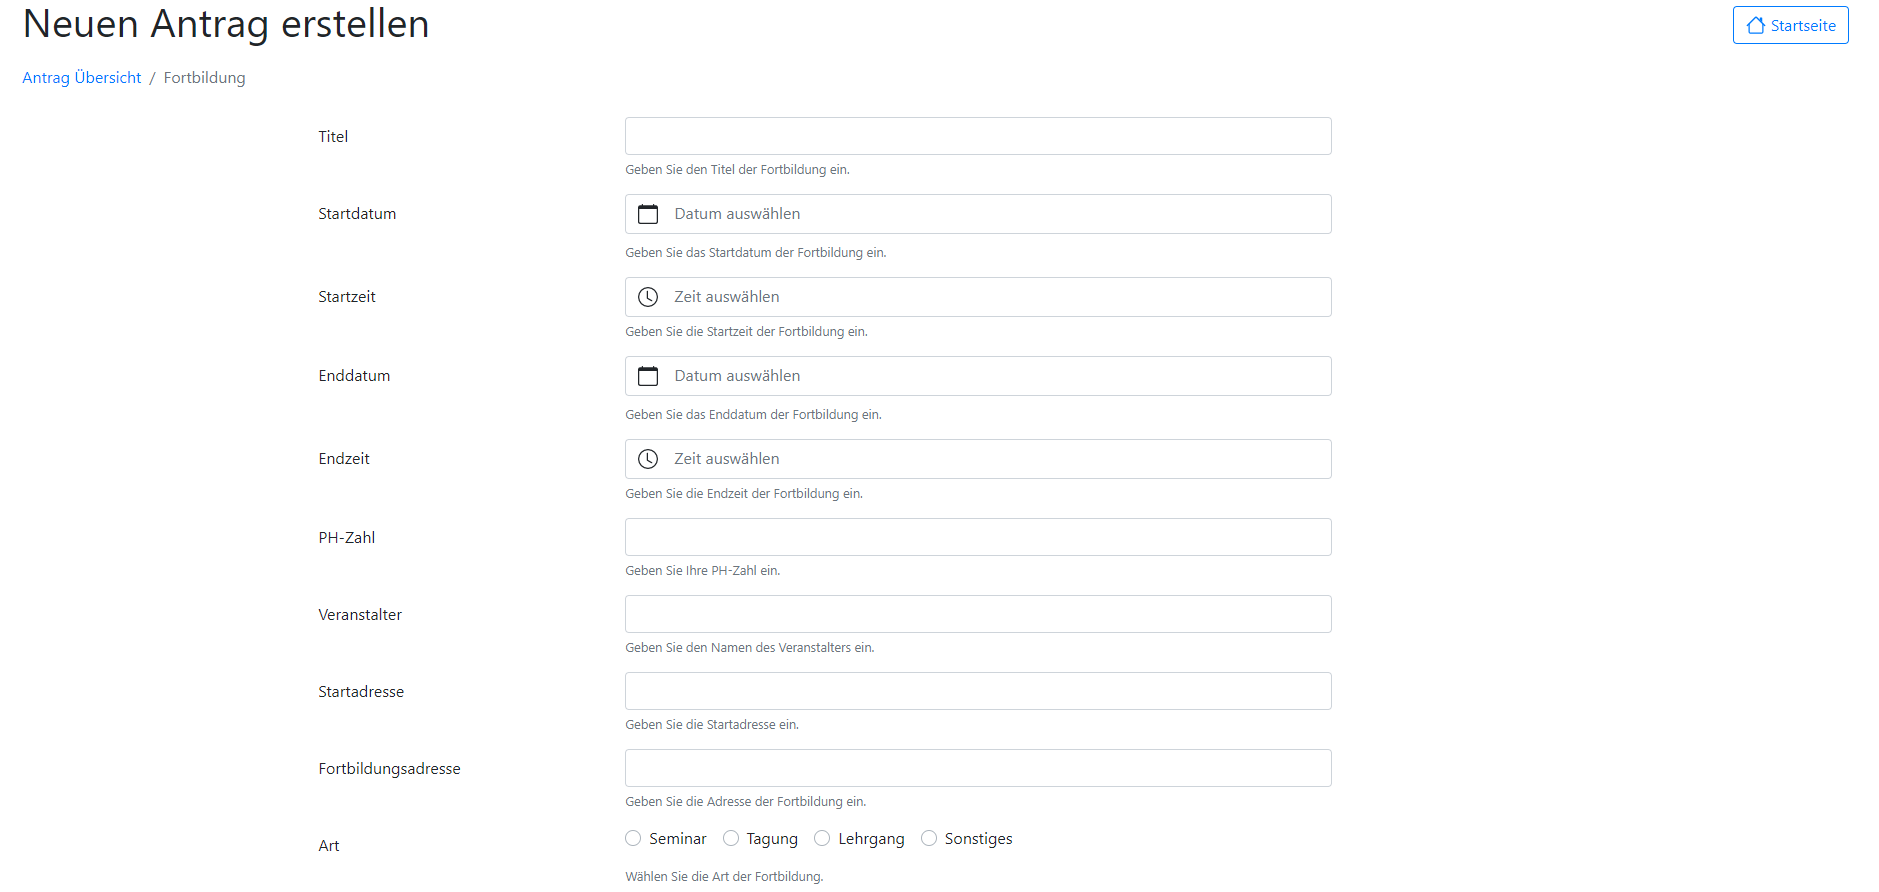
\includegraphics[width=1\linewidth]{images/website/fortbildung_1}
	\caption[Neuer Schulantrag]{Ein Bild des Begleitformulars (Teil 2)}
	\label{fig:frotbildung}
\end{figure}

\paragraph{Sonstige Anträge}
~\\
Zu den sonstigen Anträgen gehören Anliegen, wie Pflegefreistellungen, Dienstaufträge, Arzttermine und sonstige Freistellungen dieser Arten. Wählt man einen Dienstauftrag als Art aus, erscheinen automatisch noch Eingabefelder, die das Eingeben der GZ und des Titels, des Dienstauftrages ermöglichen.
\begin{figure}[H]
	\centering
	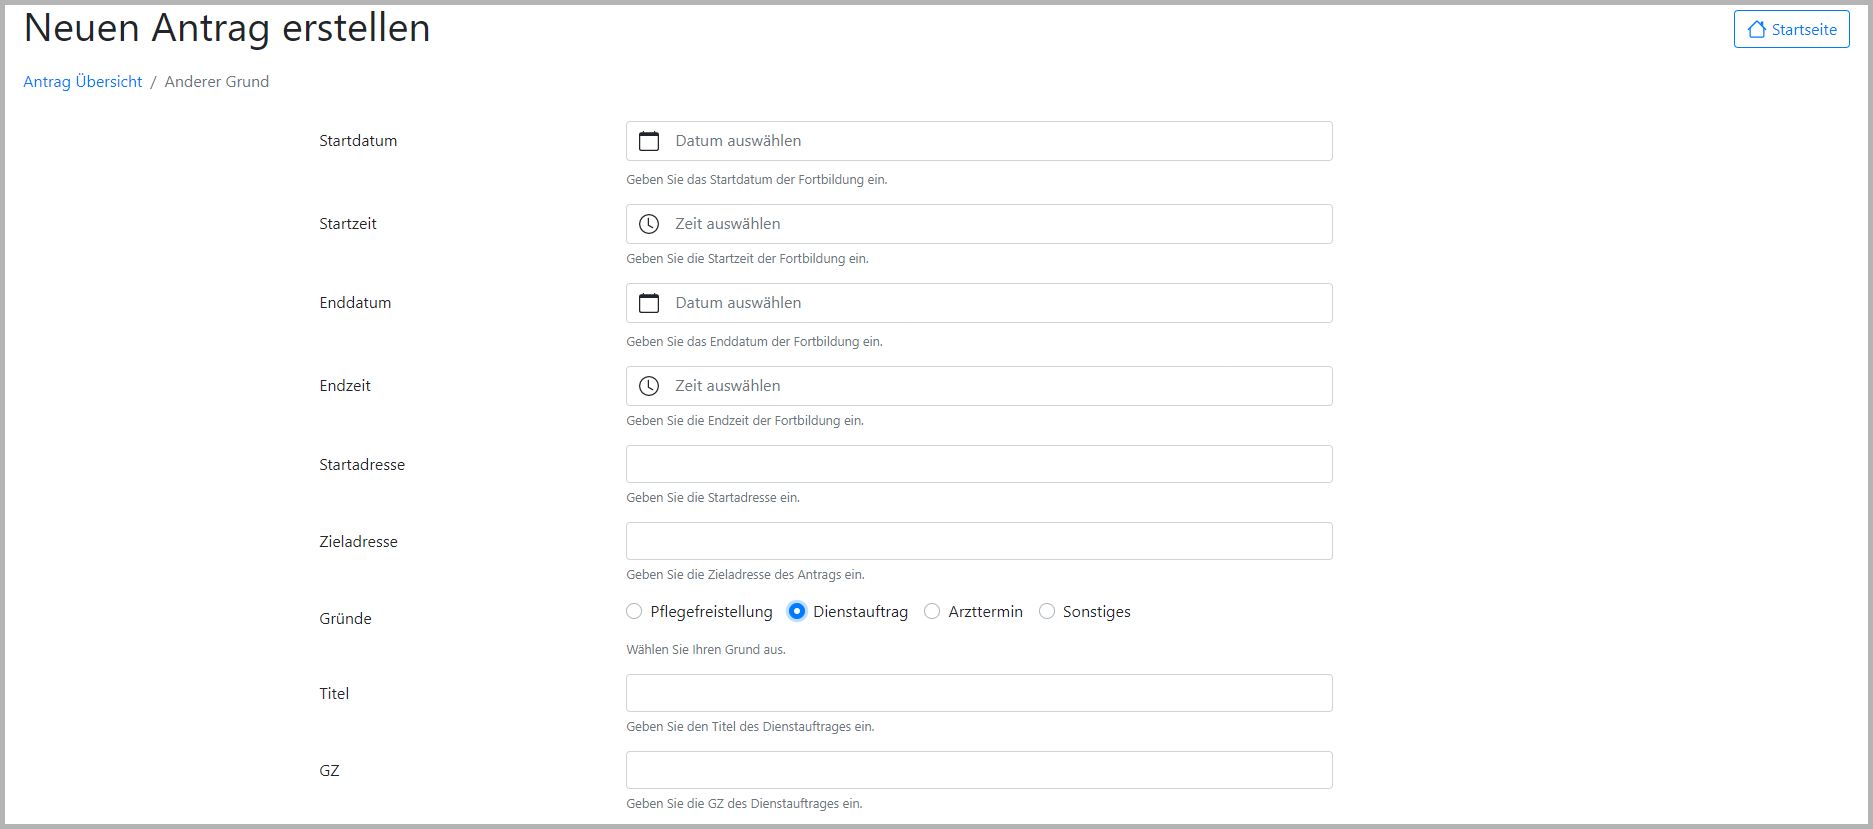
\includegraphics[width=1\linewidth]{images/website/dienstauftrag}
	\caption[Neuer Schulantrag]{Ein Bild des Begleitformulars (Teil 2)}
	\label{fig:dienst}
\end{figure}

\paragraph{Reiseantrag}
~\\
Der Reiseantrag wird automatisch bei den Formularen der Anträge angehangen, bei denen eine Reise nötig ist. Ist keine Reise für einen bestimmten Antrag (zum Beispiel ein Arztbesuch) vorgesehen, dann wird das Formular nicht angehangen und es müssen keine unnötigen Daten eingegeben werden. Die Struktur der Elemente ist ident zu denen, die bereits besprochen wurden.
\begin{figure}[H]
	\centering
	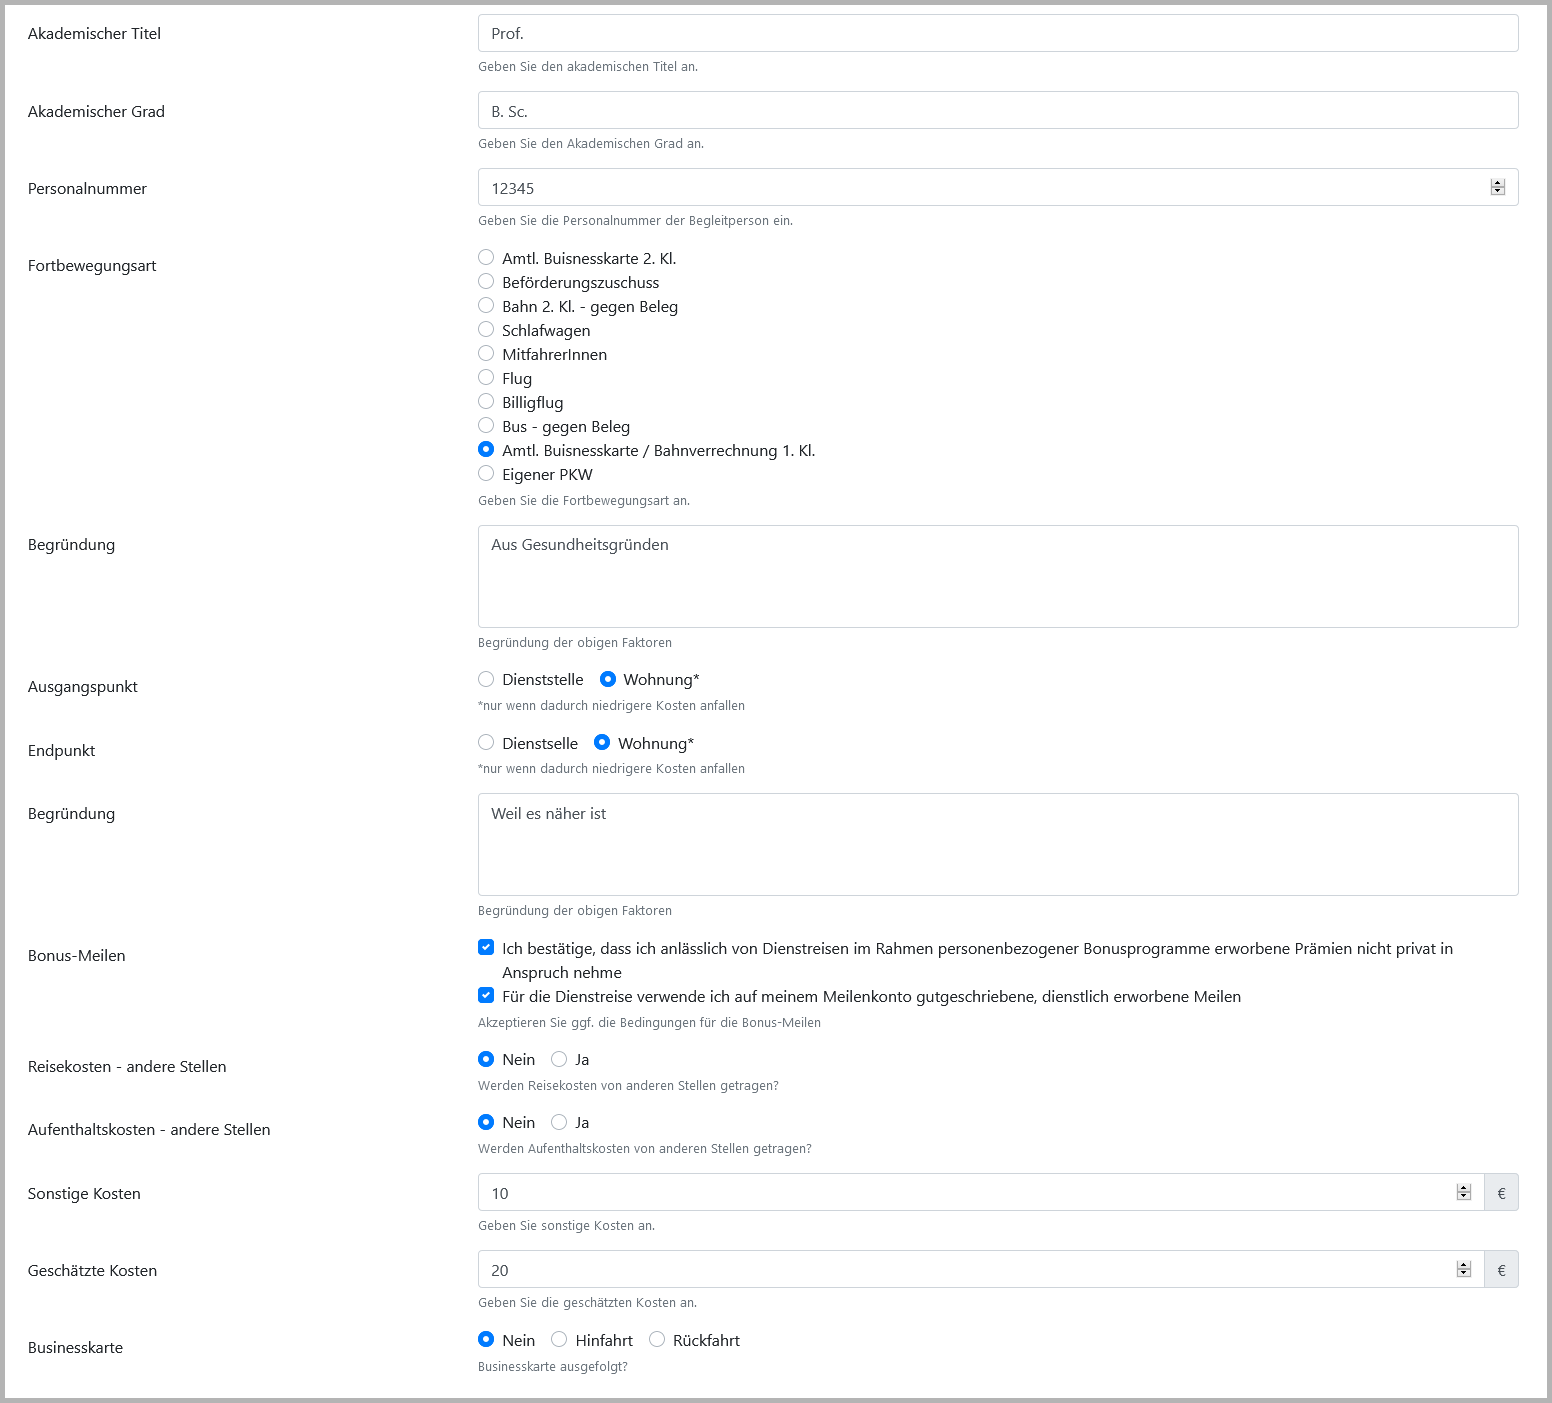
\includegraphics[width=1\linewidth]{images/website/zusatz_1}
	\caption[Neuer Schulantrag]{Ein Bild des Reiseantrages (Teil 2)}
	\label{fig:zusatz1}
\end{figure}

\subsubsection{Reisekostenabrechnung}
Das Formular der Reisekostenabrechnung fordert sehr viele verschiedene Werte von den Lehrern. Wir haben unser Bestes getan, um das Formular so einfach, wie möglich zu gestalten, jedoch ist vor allem die Tabelle mit der Berechnung der gesamten Kosten etwas komplizierter geworden. Durch die Unterstützung der Website, ist das Eingeben der Daten, aber wesentlich einfacher, als auf dem Papier, da gewisse Felder, je nach Eingabe des Benutzers, automatisch ausgegraut werden. Wenn wir uns zum Beispiel die Tabelle in folgender Abbildung anschauen, kann man nur in jene Felder schreiben, die man mit den Checkboxen angeklickt hat. Außerdem kann man direkt digital seine Belege an die Reisekostenabrechnung anhängen. Zudem wird automatisch die Zeitspanne des jeweiligen Antrages berechnet und entsprechend viele Zeilen in der Tabelle erzeugt.
\begin{figure}[H]
	\centering
	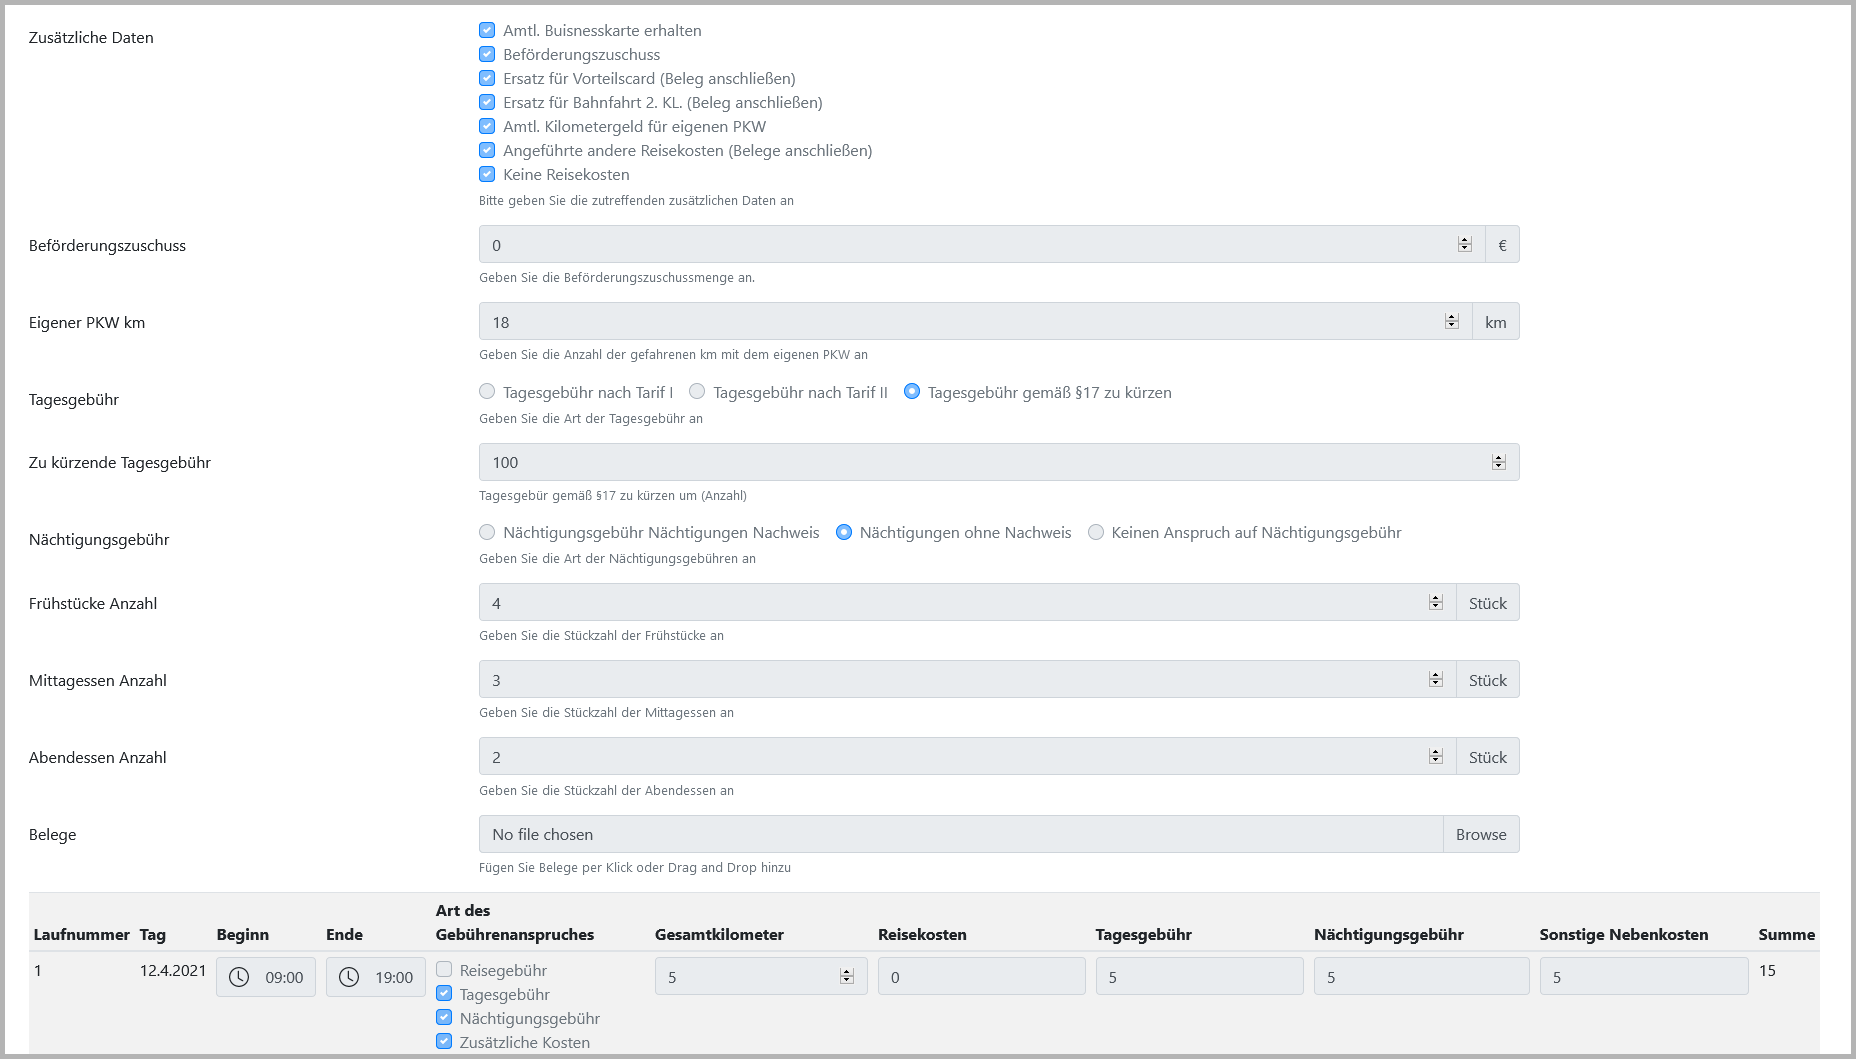
\includegraphics[width=1\linewidth]{images/website/reiserechnung_1}
	\caption[Neuer Schulantrag]{Ein Bild der Reiserechnung}
	\label{fig:reiserechnungsite}
\end{figure}
Hier wurden wieder die bekannten Elemente verwendet. Es gibt jedoch auch noch nicht verwendete Elemente, wie die Datei Auswahl und die Tabelle.
\paragraph{Datei Auswahl}
~\\
Wie auch bei den anderen Elementen der Formulare, wie zum Beispiel bei dem Timepicker, hat Bootstrap uns hier das Leben um einiges erleichtert. 
\begin{code}{html}
	<!-- Belege Input -->
	<b-form-group
	  id="belg"
	  label-cols-sm="4"
	  label-cols-lg="3"
	  content-cols-sm
	  content-cols-lg="7"
	  description="Fügen Sie Belege per Klick oder Drag and Drop hinzu"
	  label="Belege"
	  label-for="bel"
	>
	  <b-form-file
		multiple
		id="bel"
		v-model="invoices"
		v-on:input="convert"
		:disabled="readonly"
	  >
		<template slot="file-name" slot-scope="{ names }">
		  <b-badge variant="dark">{{ names[0] }}</b-badge>
		  <b-badge v-if="names.length > 1" variant="dark" class="ml-1">
			+ {{ names.length - 1 }} More files
		  </b-badge>
		</template>
	  </b-form-file>
	</b-form-group>
\end{code}
\captionof{listing}{Code - Datei auswählen}
	\label{list:dateiselect} ~\\
Wie auch andere Elemente, wird das Element zum Hochladen von Dateien in eine Eingabegruppe, mit Titel und Beschreibung eingesetzt. Nach dem Einsetzen des Elementes, kann sofort per Klick oder Drag and Drop eine, oder mehrere Dateien hinzugefügt werden. Bis die Funktionalität von dem Schnittstellen-Team hinzugefügt wurden ist, werden die Dateien nur rein optisch auf die Seite \enquote{hochgeladen}. 
\paragraph{Tabelle}
~\\
Um eine Tabelle zu erstellen, kann das Element \enquote{b-table} von Bootstrap benutzt werden. In diesem kann man direkt definieren, wie groß die Tabelle sein soll, was auf mobilen Geräten passieren soll, ob die Tabelle gestreift ist, oder nicht und so weiter. In diesem Element, haben wir dann wiederrum die verschiedenen Spalten eingebaut. Dies passiert wie folgt:
\begin{code}{html}
	<b-table
          striped
          :items="data.items"
          :fields="fields"
          stacked="md"
          show-empty
          small
    >

		...

		<template #cell(start)="data">
			<b-form-timepicker
				style="min-width: 100px;"
				id="begin"
				locale="de"
				placeholder="Zeit"
				v-model="data.item.start"
				:readonly="readonly"
				v-on:input="update()"
			></b-form-timepicker>
		</template>

		...

	</b-table>
\end{code}
\captionof{listing}{Beispielcode Tabelle}
	\label{list:bsptable} ~\\
Die Spalten werden mittels \enquote{Templates} erzeugt, danach können variabel Werte in diese Spalte, in jeder Zeile eingefügt werden. In diesem Fall befindet sich in der Zelle ein Timepicker, welcher zum auswählen der Startzeit dient.
\newpage
\subsubsection{Ansicht aktive Anträge}
Um den Lehrern das Betrachten von aktiven Anträgen einfacher zu machen, haben wir uns dazu entschlossen, eine extra Seite zu kreieren, die über das Menü auf der Startseite erreichbar ist. Hier werden alle aktiven Anträge (Ein Antrag gilt als \enquote{aktiv}, von der Antragsstellung, bis zur Rechnungsphase). Der Lehrer sieht mittels Farben (Rot: Antrag wurde abgelehnt, Gelb: Antrag wird bearbeitet, Grün: Antrag wurde angenommen) auf den ersten Blick, welchen Status der jeweilige Antrag hat. Außerdem werden in der Tabelle, der Titel des Antrages, der Leiter, das Einreichdatum und der genaue Status (In Bearbeitung, Rechnungsphase, ...) angezeigt. Falls der Lehrer viele Anträge auf einmal hat, haben wir eine Funktion zum Suchen von Anträgen im oberen Teil der Seite eingebaut. Ebenfalls ist es möglich, jede Spalte auf- und absteigend zu sortieren. Falls der Knopf namens \enquote{Antrag betrachten} betätigt wurde, kommt der Nutzer auf die \enquote{Antrags Ansicht}.
\begin{figure}[H]
	\centering
	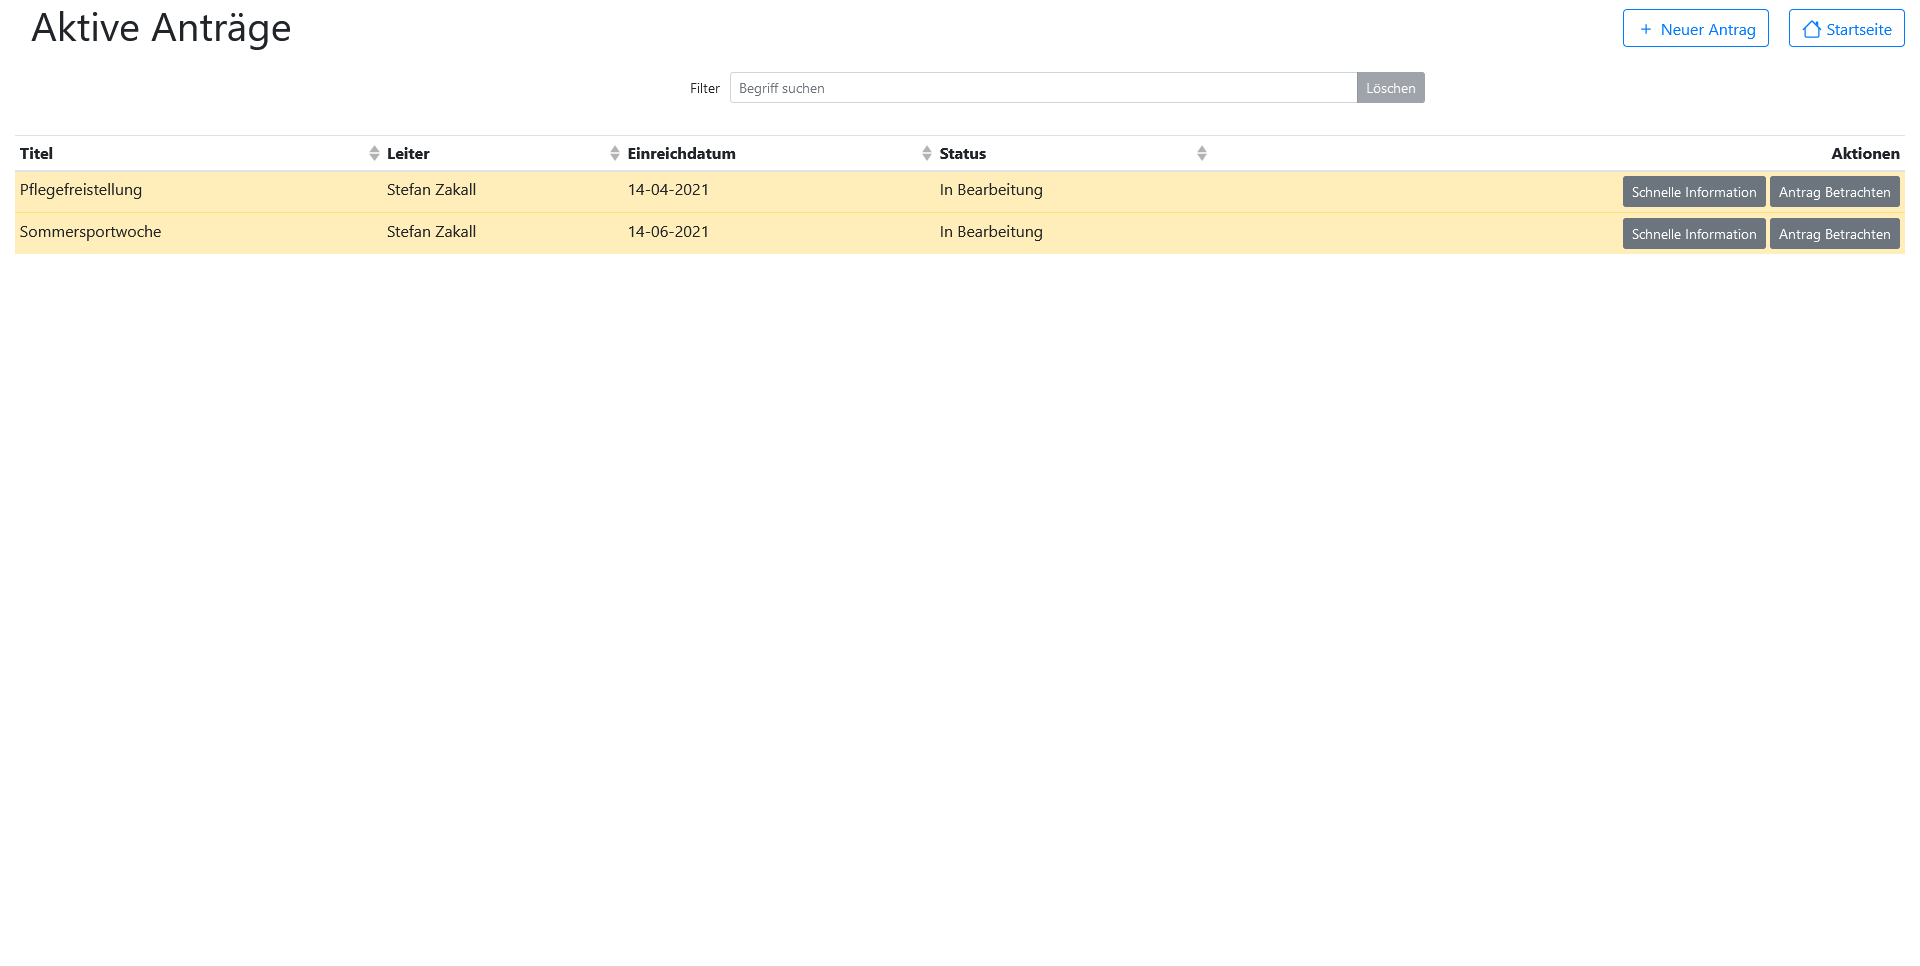
\includegraphics[width=1\linewidth]{images/website/aktiv}
	\caption[Aktiv]{Ein Bild der aktiven Anträge Seite}
	\label{fig:antragaktiv}
\end{figure}
Um die oben genannten Daten in einer geordneten Liste zu sehen kann der Lehrer auf \enquote{Schnelle Information} klicken. Dieser Vorgang öffnet folgendes Fenster:
\begin{figure}[H]
	\centering
	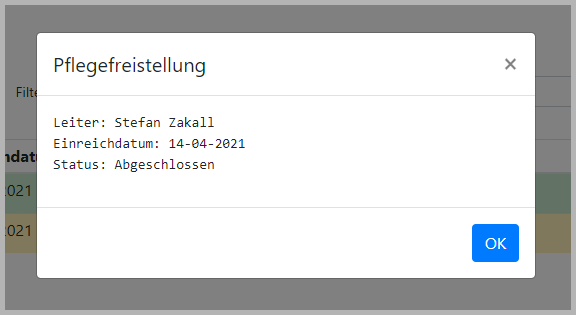
\includegraphics[width=0.6\linewidth]{images/website/aktiv_detail}
	\caption[Aktiv]{Ein Bild der Detail-Ansicht der aktiven Anträge Seite}
	\label{fig:antragaktivdetail}
\end{figure}
\paragraph{Such-Funktion}
~\\
Auch die Erstellung der Suchfunktion wurde wieder essentiell von den BootstrapVue Komponenten unterstützt. Wir mussten lediglich eine Eingabegruppe erstellen, die ein Eingabefeld mit dem Typ \enquote{search} hat. Um eine Eingabe schneller zu löschen haben wir dann noch einen Knopf hinzugefügt, der erscheint, sobald man etwas eintippt. Durch die gute Integration von Bootstrap in VueJS war die Implementierung der Suchfunktion für die Tabelle reibungslos. Die Vergabe der Funktionalität der Such-Funktion wurde im Backend/Frontend Teil durchgeführt.
\begin{code}{html}
	<!-- Such Element -->
    <b-row align-h="center" style="margin-top: 1rem; margin-bottom: 2rem">
      <b-col cols="12" md="6">
        <b-form-group
          label="Filter"
          label-for="filter-input"
          label-cols-sm="3"
          label-align-sm="right"
          label-size="sm"
          class="mb-0"
        >
          <b-input-group size="sm">
            <b-form-input
              id="filter-input"
              v-model="filter"
              type="search"
              placeholder="Begriff suchen"
            ></b-form-input>

            <b-input-group-append>
              <b-button :disabled="!filter" @click="filter = ''"
                >Löschen</b-button
              >
            </b-input-group-append>
          </b-input-group>
        </b-form-group>
      </b-col>
    </b-row>
\end{code}
\captionof{listing}{Code - Anträge Suchfunktion}
	\label{list:antragsearchcode} ~\\
\paragraph{Filterbare Tabelle}
~\\
Die Aktivierung der filterbaren Tabelle ist mittels BootstrapVue kinderleicht. Man muss lediglich folgende 3 Festlegungen im \enquote{b-table} Element hinzufügen:
\begin{code}{html}
	<b-table
		...
		:sort-by.sync="sortBy"
      	:sort-desc.sync="sortDesc"
      	:sort-direction="sortDirection"
		...
	>
	...
	</b-table>
\end{code}
\captionof{listing}{Code - Anträge filtern}
	\label{list:antragfiltercode} ~\\
\paragraph{Pop-Up Fenster}
~\\
Das Pop-Up Fenster haben wir mittels einem \enquote{Modal} von Bootstrap verwirklicht. Dieses kann über einen zugewiesenen Button geöffnet werden und beinhaltet, je nach Antrag, dessen spezifische Daten.
\begin{code}{html}
	<!-- Info modal -->
    <b-modal
      :id="infoModal.id"
      :title="infoModal.title"
      ok-only
      @hide="resetInfoModal"
    >
      <pre>{{ infoModal.content }}</pre>
    </b-modal>
\end{code}
\captionof{listing}{Code - Pop-Up Fenster}
	\label{list:codepopup} ~\\

\subsubsection{Ansicht Alle Anträge}
Diese Seite ist sehr ähnlich zu der \enquote{Aktive Anträge} Seite. Der einzige Unterschied ist, dass der Lehrer hier auch bereits abgeschlossene Anträge sieht. Auch hier haben wir die \enquote{Suchen} Funktion eingebaut, die hier eine wesentlich wichtigere Rolle spielt, als bei der Seite, der aktiven Anträge. Auch das Filtern der einzelnen Spalten ist wieder möglich.
\begin{figure}[H]
	\centering
	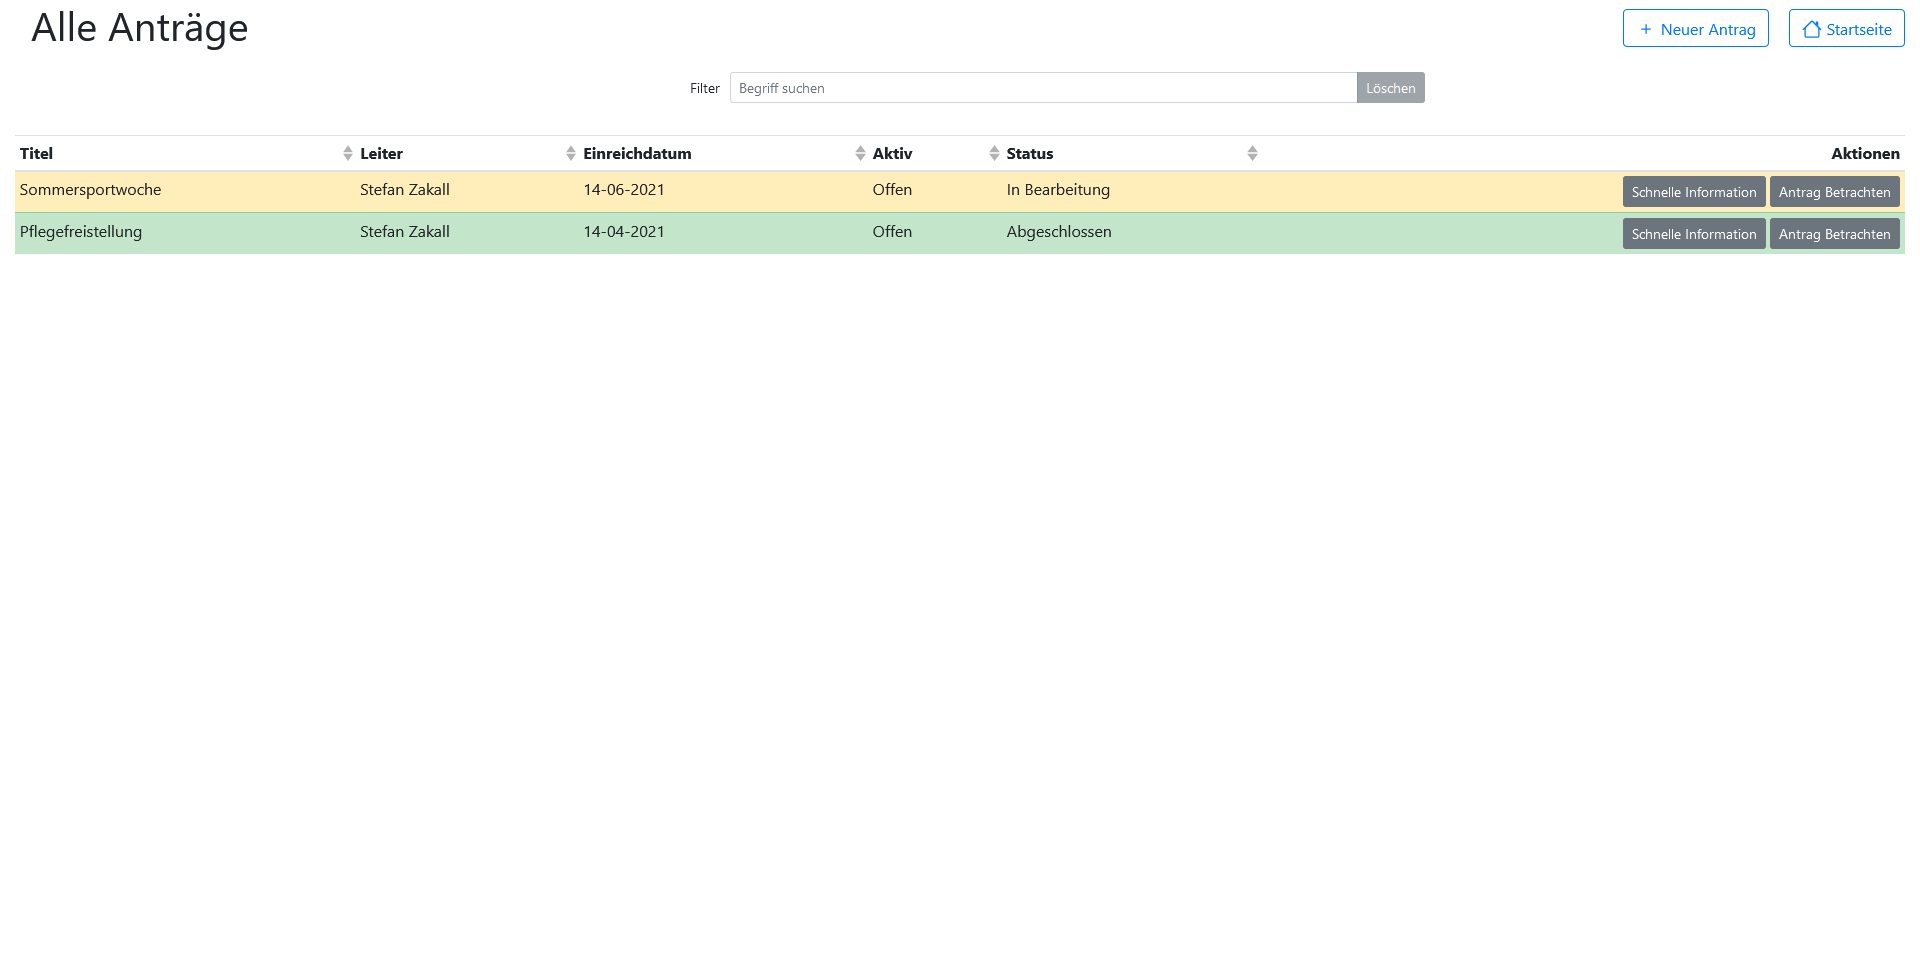
\includegraphics[width=1\linewidth]{images/website/alle}
	\caption[Aktiv]{Ein Bild der alle Anträge Seite}
	\label{fig:antragalle}
\end{figure}
~\\

\newpage
\subsubsection{Antragsansicht}
Die Antragsansicht bietet den Lehrern alle möglichen Informationen zu ihrem Antrag, die sie brauchen. Um den Lehrkräften einen besseren Überblick zu schaffen, in welcher Phase sich ihr Antrag befindet, haben wir eine Fortschrittsanzeige als erstes Element auf der Seite eingebaut. Desweiteren findet das Lehrpersonal eine aufklappbare Liste auf der Seite, in der sie je nach Status des Antrages, die Daten anzeigen und/oder editieren können. Außerdem bietet diese Seite die Funktion, eine generierte PDF von jedem Antrag zu öffnen. Falls der Lehrer Daten geändert hat, kann er diese Änderung mit einem Knopf, der sich am Schluss der Website befindet speichern. Ebenfalls ist es möglich den Antrag zu schließen, hierbei öffnet sich aber eine Warnmeldung, in der man das Schließen des Antrages nochmal bestätigen muss.
\begin{figure}[H]
	\centering
	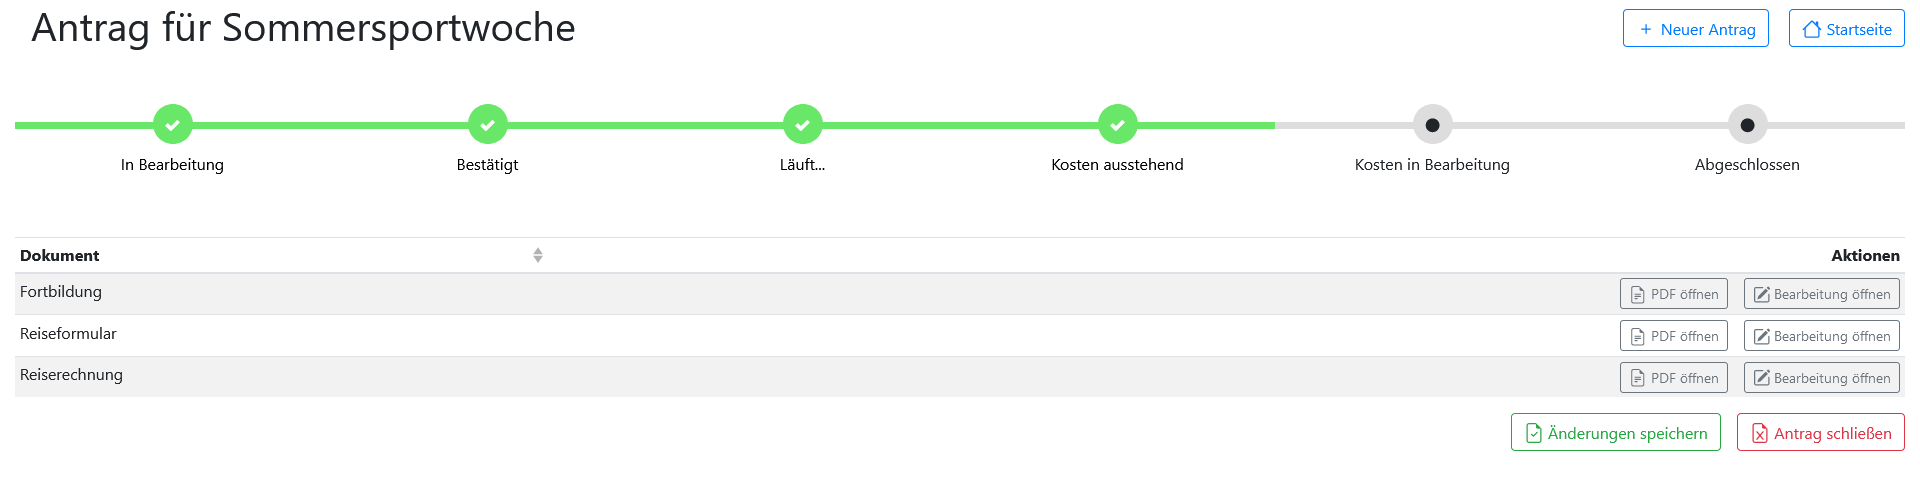
\includegraphics[width=1\linewidth]{images/website/antrag_zu}
	\caption[Aktiv]{Ein Bild der Detail-Ansicht der aktiven Anträge Seite}
	\label{fig:antragaktivdetail}
\end{figure}
\begin{figure}[H]
	\centering
	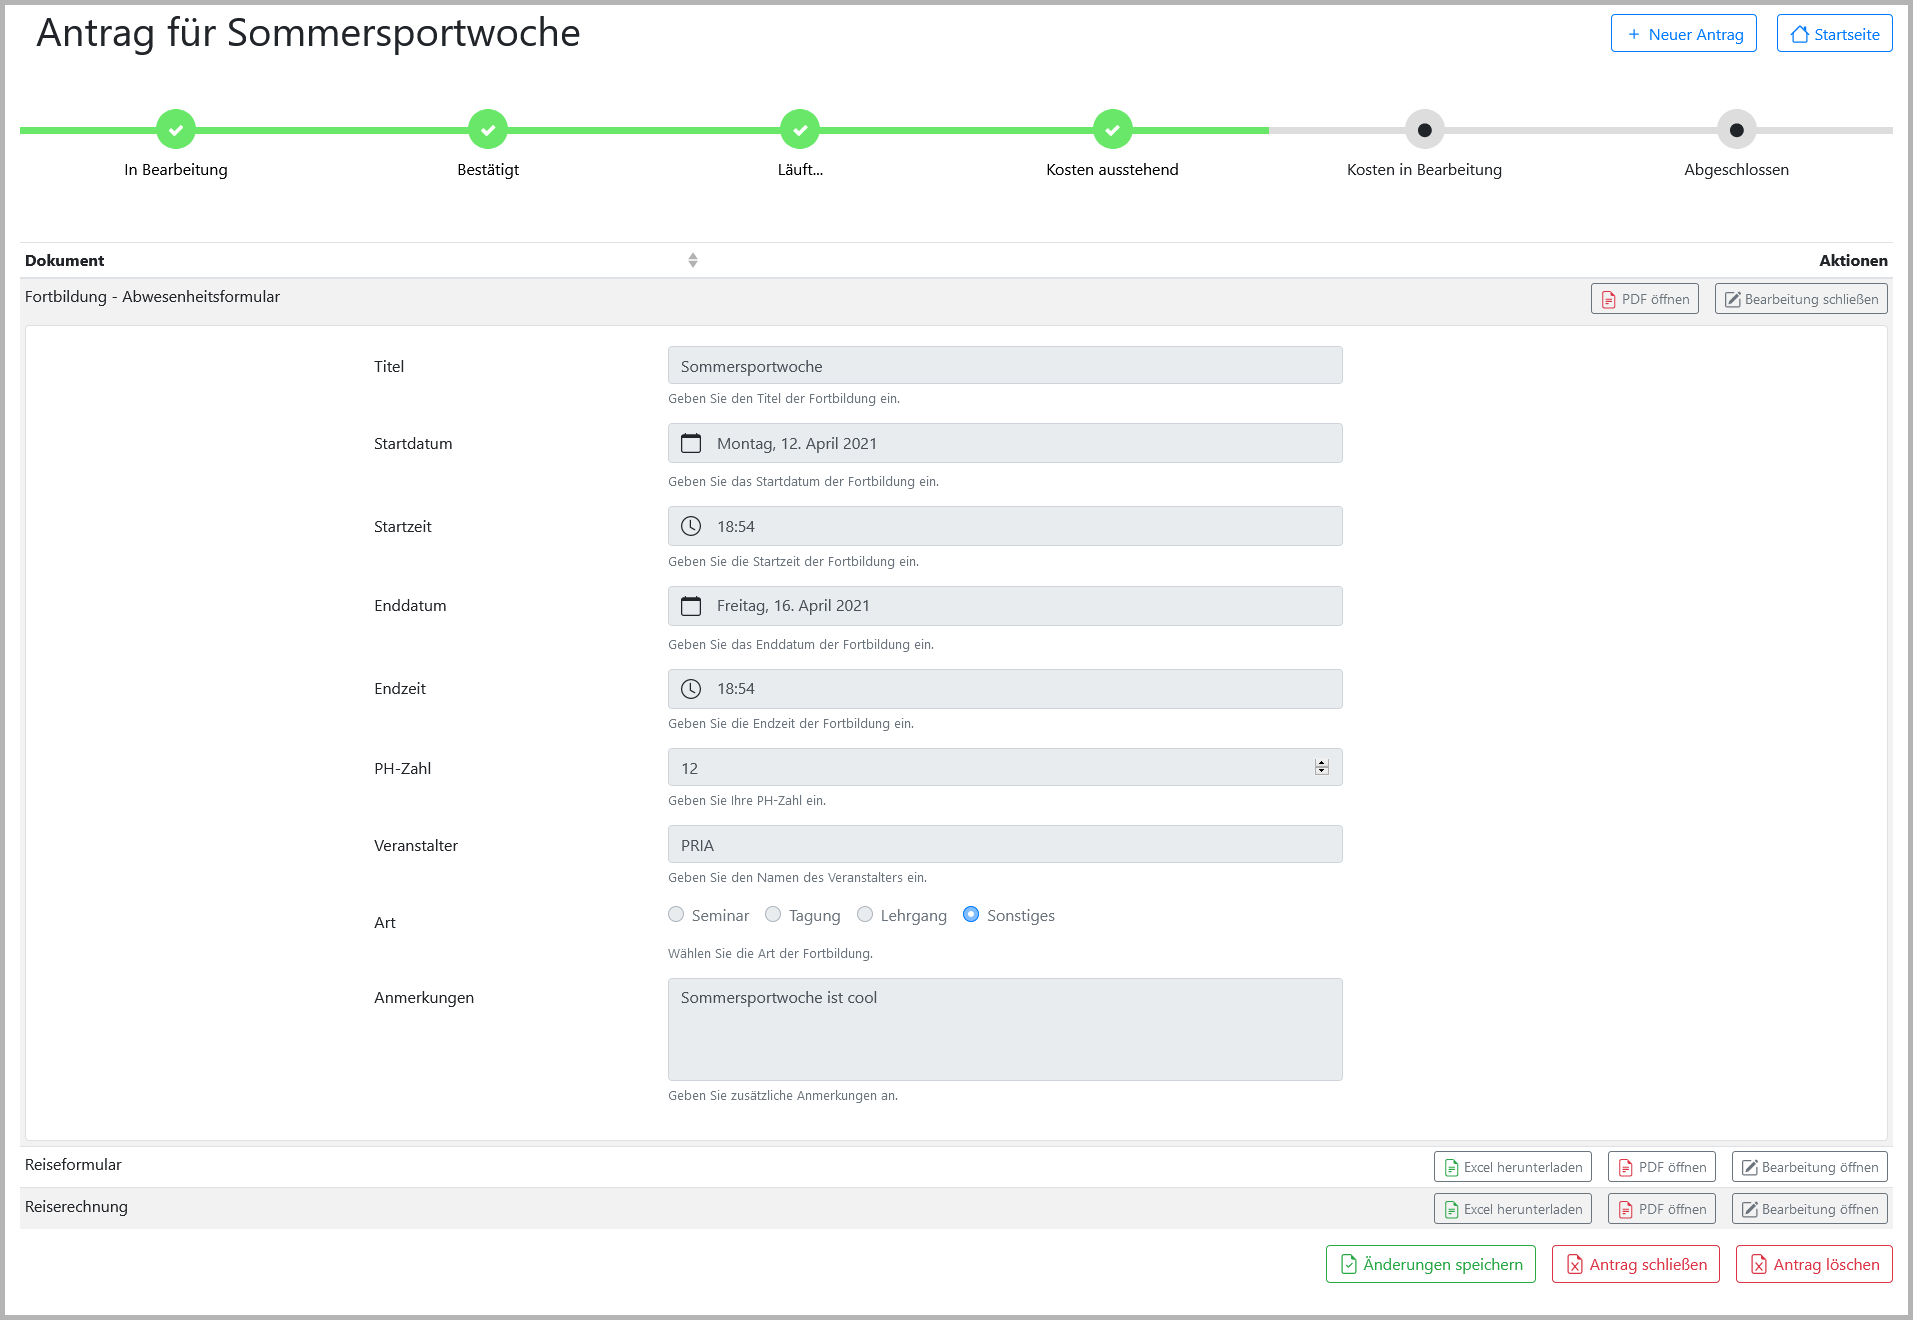
\includegraphics[width=1\linewidth]{images/website/antrag}
	\caption[Aktiv]{Ein Bild der Detail-Ansicht der aktiven Anträge Seite}
	\label{fig:antragaktivdetail}
\end{figure}
\begin{figure}[H]
	\centering
	\includegraphics[width=0.6\linewidth]{images/website/antrag_schliessen}
	\caption[Aktiv]{Ein Bild der Detail-Ansicht der aktiven Anträge Seite}
	\label{fig:antragaktivdetail}
\end{figure}

~\\
\paragraph{Fortschrittsanzeige}
~\\
Die Fortschrittsanzeige schaut sehr kompliziert aus, in Wahrheit ist sie das aber nicht. Ein Schritt der Fortschrittsanzeige besteht aus einem \enquote{div}, in dem sich ein \enquote{span} befindet. Das \enquote{div} ist ein \enquote{Strich} und in dem \enquote{span} befindet sich ein Icon, welches den Zustand beschreibt. Je nach Status des Fortschritts wird die Farbe mittels CSS-Klassen geändert.
\begin{code}{html}
	<div
            :class="{
              active: progress >= 1
            }"
            class="step"
          >
            <span class="icon">
              <i
                :class="{
                  'fa-check': progress >= 1,
                  'fa-circle': progress < 1 && progress > 0,
                  'fa-exclamation': progress == 0
                }"
                class="fa"
              ></i>
            </span>
            <span class="text text-truncate d-none d-md-block"
              >Einreichung</span
            >
          </div>
\end{code}
\captionof{listing}{Codeausschnitt - Fortschrittsanzeige}
	\label{list:codeprogress} ~\\

\begin{code}{css}
.track .step.fail:before {
  background: #ff3e3e;
}

.track .step.fail .icon {
  background: #ff3e3e;
  color: #fff;
}

.track .step.active .icon {
  background: #69e769;
  color: #fff;
}

.track .step.active:before {
  background: #69e769;
}
\end{code}
\captionof{listing}{CSS - Fortschrittsanzeige Farbklassen}
	\label{list:progresscolor} ~\\

\paragraph{Dokumente anzeigen}
~\\
Die verschiedenen Dokumente, die zu einem gewissen Antrag angehören werden in einer Tabelle gelistet. Falls man auf den \enquote{Bearbeitung öffnen} Knopf drückt, wird der Tabelle eine weitere Reihe hinzugefügt, mit allen Informationen zu dem jeweiligen Antrag. Wir verwenden mittels VueJS die bestehenden Formulare wieder (hier als Beispiel einen Schulveranstaltungsantrag), binden sie in der Tabelle ein und dann werden die Eingabefelder über die Datenschnittstelle mit Daten befüllt.
\begin{code}{html}
	<template #row-details="row">
        <b-card>
            <!-- Schulveranstaltung -->
            <SchoolGeneral
            v-bind:readonly="sgreadonly"
            v-bind:data="app"
            v-bind:token="token"
            v-bind:url="url"
            v-on:update="updateSG"
            v-if="isLeader && row.item.title == 'Allgemeine Infos'"
            />
		</b-card>
	</template>
\end{code}
\captionof{listing}{Code - Dokumente anzeigen}
	\label{list:docanz} ~\\

\paragraph{Funktionen}
~\\
Wird der \enquote{Antrag schließen} Knopf betätigt, erscheint eine Sicherheitsmeldung. Diese wird mit einem \enquote{Modal} erstellt, welches einen Text beinhaltet, der den Lehrer vor den Folgen dieser Tat warnt und zwei weitere Knöpfe. Einen grünen Knopf, um den Vorgang abzubrechen und einen roten Knopf, der einen rot blinkenden \enquote{Spinner} beinhaltet, um den Lehrkräften klar zu machen, dass man sich das Schließen, des Antrages gut überlegen sollte.
\begin{code}{html}
	<!-- Sicherheitshinweis Antrag schließen -->
    <b-modal ref="close-modal" hide-footer title="Antrag schließen">
      <b-container fluid>
        <b-row
          ><b-col cols="12">
            <div class="d-block text-center">
              <p>
                Sind Sie sich sicher, dass Sie den Antrag schließen wollen? Er
                wird danach nicht mehr für die Prüfer sichtbar sein und
                <b>kann nicht mehr geöffnet werden!</b>
              </p>
            </div>
          </b-col></b-row
        >
        <b-row>
          <b-col cols="6">
            <!-- Antrag schließen bestätigung -->
            <b-button class="mt-2" variant="outline-danger" block @click="delAn"
              >Antrag schließen <b-spinner small type="grow"></b-spinner
            ></b-button>
          </b-col>
          <b-col cols="6">
            <!-- Abbrechen Button --><b-button
              class="mt-2"
              variant="outline-success"
              block
              @click="hideClose"
              >Abbrechen</b-button
            ></b-col
          >
        </b-row>
      </b-container>
    </b-modal>
\end{code}
\captionof{listing}{Code - Antrag schließen Sicherheitshinweis}
	\label{list:securityalert} ~\\
~\\

\newpage
\subsubsection{Administrator Ansicht}
Die Administratoransicht ist wie die \enquote{alle Anträge} oder \enquote{aktive Anträge} Ansicht der Lehrer mit der Struktur einer Tabelle aufgebaut und hat eine Such- als auch Filterfunktion. Eine Zusatzfunktion, die es gibt ist, dass man direkt in der Übersicht, einen oder mehrere Anträge auswählen kann und diese direkt als PDFs exportieren kann. Außerdem sehen die Admitistratoren auf den ersten Blick wesentlich mehr Informationen, als normale Nutzer. Es wird der Titel des Antrages angezeigt, die Art, das Enreichdatum, für wann der Antrag ist, den Status (je nach Status sehen gewisse Rollen die Anträge) und den Antragssteller in Kurzschreibweise. Auch hier ist es wieder möglich die Antragsansicht zu öffnen.
\begin{figure}[H]
	\centering
	\includegraphics[width=1\linewidth]{images/website/admin}
	\caption[Aktiv]{Ein Bild der Admin Ansicht}
	\label{fig:adminview}
\end{figure}
Die farbig hinterlegten Elemente heißen \enquote{badges} und können wie folgt erstellt werden:
\begin{code}{html}
	<b-badge variant="danger">Rote Badge</b-badge>
	<b-badge variant="success">Grüne Badge</b-badge>
	<b-badge>Graue Badge</b-badge>
\end{code}
\captionof{listing}{Code - Badge Beispiel}
	\label{list:badgebsp} ~\\
~\\

\newpage
\paragraph{Administrator Antragsansicht}
~\\
Die Administrator Antragsansicht schaut exakt gleich aus, wie die Ansicht der Lehrer - mit einem Unterschied. Die Administratoren haben nicht die Funktionen \enquote{Speichern} und \enquote{Antrag schließen}, sondern \enquote{Antrag annehmen} und \enquote{Antrag ablehnen}. Falls der Antrag abgelehnt wird taucht wieder eine Sicherheitsmeldung auf. Hier muss der Administrator eine Begründung, für die Ablehnung angeben. 
\begin{figure}[H]
	\centering
	\includegraphics[width=0.6\linewidth]{images/website/admin_antrag_schiessen}
	\caption[Aktiv]{Ein Bild der Antrag ablehnen Meldung}
	\label{fig:adminclose}
\end{figure}
Im Code wird dieses Eingabefeld im \enquote{Modal} wie folgt erstellt:
\begin{code}{html}
	<!-- Antrag Ablehnen Warnhinweis -->
    <b-modal ref="close-modal" hide-footer title="Antrag ablehnen">
      <b-container fluid>
        <b-row
          ><b-col cols="12">
            <div class="d-block text-center">
              <p>
                Sind Sie sich sicher, dass Sie den Antrag ablehnen wollen?
              </p>
              <!-- Begründung der Ablehnung -->
              <b-form-textarea
                id="decline-reason"
                placeholder="Begründung"
                rows="3"
                no-resize
              ></b-form-textarea>
            </div> </b-col
        ></b-row>
        <b-row>
          <b-col cols="6">
            <!-- Antrag ablehnen Bestätigung -->
            <b-button class="mt-2" variant="outline-danger" block @click="delAn"
              >Antrag ablehnen <b-spinner small type="grow"></b-spinner
            ></b-button>
          </b-col>
          <b-col cols="6">
            <!-- Abbrechen Button -->
            <b-button
              class="mt-2"
              variant="outline-success"
              block
              @click="hideClose"
              >Abbrechen</b-button
            ></b-col
          >
        </b-row>
      </b-container>
    </b-modal>
\end{code}
\captionof{listing}{Code - Antrag ablehnen}
	\label{list:badgebsp} ~\\
\newpage
\subsubsection{Seite nicht Gefunden}
Falls der momentane Nutzer von Refundable eine ungültige URL aufruft, wollten wir diesem sofort klar machen, dass er etwas falsch gemacht hat. Desweiteren wollten wir dem Nutzer direkt eine Lösung vorschlagen, wie er dieses Problem beheben kann - ein \textit{Button}, der den Nutzer wieder zur Startseite bringt. Um dem Nutzer zu visualisieren, dass dieser Knopf die richtige Wahl ist, haben wir ihn in einem Grün hervorgehoben. Außerdem wird dem Aufrufer, der Seite mit schimmernden grauen Boxen, die einen \enquote{Lade-Zustand} visualisieren sollen gezeigt, dass die Seite, die der Nutzer aufrufen wollte nicht richtig lädt.
\begin{figure}[H]
	\centering
	\includegraphics[width=1\linewidth]{images/website/notfound}
	\caption[Neuer Schulantrag]{Ein Bild der nicht Gefunden Seite}
	\label{fig:notfoundsite}
\end{figure}
~\\
Die Elemente, welche den Lade-Zustand verkörpern sollen heißen \enquote{b-skeleton-img} und werden wie folgt erstellt:
\begin{code}{html}
	<b-skeleton-img animation="fade"></b-skeleton-img>
\end{code}
\captionof{listing}{Code - Skeleton}
	\label{list:codeskeleton} ~\\

\newpage
\subsubsection{Antrag suchen}
Um den Administratoren während ihren Tätigkeiten ein wenig Arbeit abzunehmen, haben wir eine Möglichkeit eingebaut, einen Antrag direkt über eine Seite zu suchen. Dazu muss der Administrator nur die Unterseite \enquote{/viewer} aufrufen und kann, wie man in Abbildung 7.13 sehen kann, die Antrags ID suchen und so direkt zu dem gewünschten Antrag gelangen.
\begin{figure}[H]
	\centering
	\includegraphics[width=1\linewidth]{images/website/search}
	\caption[Neuer Schulantrag]{Ein Bild der Antrag suchen Seite}
	\label{fig:searchsite}
\end{figure}
~\\

\newpage 
\subsubsection{Rechte vergeben}
Während der Entwicklung ist uns aufgefallen, dass die Funktion fehlt, einem bestimmten Benutzer gewisse Rechte zu geben. Daher ist es dem \textit{Superuser} möglich über das Admindashboard Rechte zu vergeben. Dazu muss er nur die E-Mail der bestimmten Person eingeben und kann mittels \textit{Radio-Buttons} die gewünschten Rechte auswählen. Auch hier wurden wieder die bekannten Elemente der restlichen Website verwendet.
\begin{figure}[H]
	\centering
	\includegraphics[width=1\linewidth]{images/website/rechte}
	\caption[Neuer Schulantrag]{Ein Bild der Rechte vergeben Seite}
	\label{fig:rightssite}
\end{figure}
\lfoot{Michael Beier}
%!TEX root=../../main.tex

\section{Backend und Infrastruktur}

\subsection{Einleitung}
Wie im Konzept (in \autoref{chapter:conceptbi}) zuvor ausführlich beschrieben soll eine den Plänen entsprechende automatisch aufbaubare Infrastruktur erstellt und ein dem System angepasstes Backend programmiert werden. Hierfür wurde bereits in der Studie (in \autoref{chapter:golanganalyse}) Golang als zu benutzende Sprache ausgewählt.
\subsection{Docker}

In den folgenden Kapiteln wird die genaue Umsetzung der einzelnen Docker-Images, jeweils definiert in Dockerfiles, des Docker-Compose Stack und des Aufbaus der Volumen, Umgebungsvariablen und Secrets beschrieben.

\subsubsection{MongoDB}

Das Dockerfile in der \autoref{code:dockermongo} beschreibt die Datenbank, eine MongoDB Instanz, die einen eigenen Container erhält. Das aus dem Dockerfile resultierende Image basiert auf der neuesten Version des offiziellen mongo-Images, welches die eigentliche MongoDB-Instanz beinhaltet. Des Weiteren wird das Initskript hinzugefügt, sodass dieses beim Erstellen des Containers immer ausgeführt wird. Zuletzt wird noch der Port 27017, der Standard Port der MongoDB Anwendung, nach außen hin freigegeben.

\begin{minted}{Dockerfile}
FROM mongo:latest

ADD ./init-db.sh /docker-entrypoint-initdb.d/

EXPOSE 27017
\end{minted}
\captionof{listing}[MongoDB Dockerfile]{MongoDB Dockerfile}
\label{code:dockermongo}
~\\
Das Bashskript in der \autoref{code:mongoskript} sorgt für die Erstellung eines Nutzers als Administrator, einer Datenbank und eines weiteren Benutzers mit einfacher Lese- und Schreibberechtigung. Dieser Vorgang ist nötig, damit die Datenbank direkt verwendbar ist, und nicht erst eine Datenbank von der Seite des Programmes aus erstellt werden muss. Der weitere User stellt ein Best-Practice da, indem man den User, mit welchen man jegliche Daten schreibt, nicht alle Berechtigungen zuschreibt, sondern lediglich jene, die er wirklich braucht. 

\newpage

\begin{minted}{bash}
#!/bin/bash

mongo -- "$MONGO_DATABASE" << EOF
	var rootUser = '$(cat "$MONGO_INITDB_ROOT_USERNAME_FILE")';
	var rootPassword = '$(cat "$MONGO_INITDB_ROOT_PASSWORD_FILE")';
	var admin = db.getSiblingDB("$MONGO_INITDB_DATABASE");
	admin.auth(rootUser, rootPassword);

	var user = '$(cat "$MONGO_USERNAME_FILE")';
	var passwd = '$(cat "$MONGO_PASSWORD_FILE")';
	db.createUser({user: user, pwd: passwd, roles: ["readWrite"]});
EOF
\end{minted}
\captionof{listing}[MongoDB Initskript]{MongoDB Initskript}
\label{code:mongoskript}
~\\
Die \autoref{code:mongocompose} zeigt wie das eigens definierte MongoDB Image weiterverwendet wird, speziell wie die verschiedenen Nutzerinformationen in den Container weitergegeben werden. Dies geschieht über Secrets. \cite{secretmongo} Hierbei handelt es sich um einfache Dateien, welche sicher in den Container eingehängt und dann darin ausgelesen werden können. In diesem Fall werden die Dateien durch den Installationsvorgang des Systems erstellt. 

\begin{minted}{yaml}
mongo:
	build: images/mongo/
	container_name: 'mongo-database'
	restart: always
	ports:
		- '27017:27017'
	volumes:
		- './volumes/mongo/:/data/db/'
	environment:
		MONGO_INITDB_ROOT_USERNAME_FILE: '/run/secrets/mongodb_root_username'
		MONGO_INITDB_ROOT_PASSWORD_FILE: '/run/secrets/mongodb_root_password'
		MONGO_INITDB_DATABASE: 'admin'
		MONGO_USERNAME_FILE: '/run/secrets/mongodb_username'
		MONGO_PASSWORD_FILE: '/run/secrets/mongodb_password'
		MONGO_DATABASE: 'refundable'
	secrets:
		- mongodb_root_username
		- mongodb_root_password
		- mongodb_username
		- mongodb_password
\end{minted}
\captionof{listing}[Docker-Compose File: MongoDB-Container]{Docker-Compose File: MongoDB-Container}
\label{code:mongocompose}

\newpage

\subsubsection{Backend}

Im Golang-Backend, welches in der \autoref{code:backgodocker} beschrieben wird, läuft nicht nur das Backend selbst, sondern es wird auch kompiliert. Dies bringt den Vorteil mit sich, dass es automatisch für das von Docker bereitgestellte System kompiliert wird und es also keine Auslieferung von bereits kompilierten Dateien braucht. Es wird hier ein neues Image gebaut, woraufhin in den Go-Path die Quellcodedateien hineinkopiert werden. Danach werden alle benötigten Dependencies heruntergeladen und das dann vollständige Projekt wird kompiliert. Nachdem der Port 8080 freigegeben wurde, wird das fertig kompilierte Programm gestartet.

\begin{minted}{Dockerfile}
FROM golang:1.14
	
WORKDIR /go/src/huginn
COPY . .
	
RUN go get -d -v ./...
RUN go install -v ./...
	
EXPOSE 8080
	
CMD ["huginn"]
\end{minted}
\captionof{listing}[Backend Dockerfile]{Backend Dockerfile}
\label{code:backgodocker}
~\\
Dieses Docker-Image ist auch ein Teil des Docker-Stacks und somit ist es auch in der Docker-Compose Konfiguration vorhanden (\autoref{code:golangbackendcompose}). Hier werden verschiedene Volumen eingehängt, um Dateien, wie die generierten Formulare, oder Secrets zum Signieren von Tokens, permanent zu speichern. Außerdem werden wieder die selben Secrets, die im MongoDB Container, die Nutzerinformationen des Datenbanknutzers gespeichert hatten, hinzugefügt. \cite{secretmongo} Dies ist darauf zurückzuführen, dass diese gleich durch das Backend wiederverwendet werden, um sich mit dem Nutzer einloggen zu können.

\begin{minted}{yaml}
rest:
	build: src/huginn/
	container_name: 'rest-api-backend'
	ports:
		- '8080:8080'
	volumes:
		- './volumes/secrets/:/vol/secrets/'
		- './volumes/files/:/vol/files/'
	environment:
		MONGO_USERNAME_FILE: '/run/secrets/mongodb_username'
		MONGO_PASSWORD_FILE: '/run/secrets/mongodb_password'
		MONGO_DATABASE: 'refundable'
	secrets:
		- mongodb_username
		- mongodb_password
\end{minted}
\captionof{listing}[Docker-Compose File: Backend-Container]{Docker-Compose File: Backend-Container}
\label{code:golangbackendcompose}

\newpage

\subsubsection{Frontend}

Zuletzt wird noch das Frontend in \autoref{code:dockerfrontend} definiert. Hierbei wird ein ähnlicher Zugang wie mit dem Backend gewählt, sodass auch das Frontend erst in einem Docker-Container kompiliert wird. Dies ist nicht so einfach, wie im Backend, da eine eigene Node.js Umgebung hierfür benötigt wird. Aus diesem Grund baut das Image grundsätzlich mal so eine auf und ladet darin die entsprechenden Dependencies herunter. Diese werden dann kompiliert. Das fertig kompilierte Frontend wird dann in einen anderen Docker-Container verschoben, welcher den eigentlichen Webserver umfasst, der das Frontend dann bereit stellt. Der nginx-Webserver wird nachdem er den Port 80 freigegeben hat noch formell gestartet.

\begin{minted}{Dockerfile}
FROM node:lts-alpine AS vue-builder
WORKDIR /app
COPY package*.json ./
RUN npm install
COPY . .
RUN npm run build
	
FROM nginx:stable-alpine as production
COPY --from=vue-builder /app/dist /usr/share/nginx/html
COPY history.conf /etc/nginx/conf.d/history.conf
EXPOSE 80
CMD ["nginx", "-g", "daemon off;"]
\end{minted}
\captionof{listing}[Frontend Dockerfile]{Frontend Dockerfile}
\label{code:dockerfrontend}
~\\
Auch dieses Image muss in der Docker-Konfiguration hinzugefügt werden. Dies wird durch die in \autoref{code:frontendcompose} aufgeführten Konfigurationen erreicht. Hierbei werden lediglich die entsprechenden Ports festgelegt, mehr Informationen, wie beispielsweise Secrets braucht der Webserver nicht.

\begin{minted}{yaml}
web:
	build: src/web/
	container_name: 'frontend-nginx-webapp'
	ports:
		- '80:80'
		- '443:443'
\end{minted}
\captionof{listing}[Docker-Compose File: Web-Container]{Docker-Compose File: Web-Container}
\label{code:frontendcompose}

\newpage

\subsubsection{Secrets}

Nachdem nun die verschiedenen Images, aus denen der Docker-Compose Stack bestehen soll, konfiguriert und in die zentrale Docker-Compose Datei hinzugefügt wurden, müssen zuletzt noch die benutzten Secrets registriert werden. \cite{secretmongo} Dies erfolgt wie in \autoref{code:dockersecrets} ersichtlich. Der Name des Secrets wird einer Datei zugeordnet, diese Datei wird dann, wie bereits erwähnt, in den entsprechenden Containern eingehängt. Hierdurch lässt sich einfach die bei der Installation eingelesenen Daten in die Container weitergeben.

\begin{minted}{yaml}
secrets:
	mongodb_root_username:
		file: config/mongodb_root_username
	mongodb_root_password:
		file: config/mongodb_root_password
	mongodb_username:
		file: config/mongodb_username
	mongodb_password:
		file: config/mongodb_password
\end{minted}
\captionof{listing}[Docker-Compose File: Secrets]{Docker-Compose File: Secrets}
\label{code:dockersecrets}

\subsection{Steuerungsskript}
\subsubsection{Docker Installation}

Bei der Docker Installation, welche in \autoref{code:dockerinstall} ersichtlich ist, wird Docker und Docker-Compose während des Installationsvorganges installiert, sofern dies so angegeben ist. Hierfür existiert der Parameter -d. Ist dieser vorhanden, so wird das offizielle Docker-Installer Skript heruntergeladen und ausgeführt. Danach wird noch Docker-Compose installiert. Dies geschieht durch das Herunterladen des eigentlichen Programms und der anschließenden Rechtezuteilung zur Ausführung dessen.

\begin{minted}{bash}
if [ "$1" = "-d" ]; then
	printf "Downloading Docker.\n"
	curl -fsSL get.docker.com -o docker-install.sh > /dev/null
	printf "Download complete. Now installing. This may take a while.\n"
	sudo sh docker-install.sh
	rm docker-install.sh
	printf "\n------\n\n"
	printf "Downloading Docker-Compose.\n"
	sudo curl -L "https://github.com/docker/compose/releases/download/1.27.4/docker-compose-$(uname -s)-$(uname -m)" -o /usr/local/bin/docker-compose
	printf "Download complete.\n"
	sudo chmod +x /usr/local/bin/docker-compose
	printf "Docker and Docker Compose installed successfully.\n"
	printf "\n------\n"
fi
\end{minted}
\captionof{listing}[Docker Installation - Steuerungsskript]{Docker Installation - Steuerungsskript}
\label{code:dockerinstall}

\subsubsection{Installation}

In der \autoref{code:installer} ist der Installationsvorgang ersichtlich. Der Kommentar signalisiert, wo die Docker-Installation eigentlich in der Methode stehen würde. Der Installationsvorgang gliedert sich in zwei Teile. Im ersten werden alle Git-Repositories automatisch geklont. Dadurch wurden nun alle Quellcodedateien, welche nach dem Starten in etwaigen Docker-Containern enden würden, heruntergeladen. Zusätzlich wird der Nutzer nun auch noch die Nutzerinformationen des Datenbankadministrators und des Datenbanknutzers gefragt. Diese Informationen werden in die entsprechenden Dateien gespeichert, sodass sie danach von Docker als Secrets genutzt werden können. Zuletzt wird sowohl im Backend als auch im Frontend die Adresse benötigt unter welcher der Server erreichbar ist. Diese URL wird jeweils in eine dafür vorgesehene Datei im Backend und Frontend gespeichert, sodass diese auslesbar sind.

\begin{minted}{bash}
sub_install() {
	# Docker Installation
	mkdir src/
	printf "Downloading the Backend (huginn).\n"
	git clone --quiet https://github.com/refundable-tgm/huginn.git src/huginn > /dev/null
	printf "Download complete\nDownloading the Frontend (web).\n"
	git clone --quiet https://github.com/refundable-tgm/web.git src/web > /dev/null
	printf "Download complete.\n"
	printf "\n------\n\n"
	read -rp "Choose a MongoDB Admin Username: " adminusername
	read -srp "Choose a MongoDB Admin Password: " adminpassword
	printf "\n"
	read -rp "Choose a MongoDB Username: " username
	read -srp "Choose a MongoDB User Password: " userpassword
	echo "$adminusername" > config/mongodb_root_username
	echo "$adminpassword" > config/mongodb_root_password
	echo "$username" > config/mongodb_username
	echo "$userpassword" > config/mongodb_password
	printf "\n"
	read -rp "Input the URL (without port, this is will be 8080 by default):" url
	printf '{\n\t"url":"%s"\n}' "$url" > src/web/src/data.json
	echo "$url" > volumes/files/.url
	printf "\n"
	read -rp "Input the name of the initial super user" superuser
	echo "$superuser" > volumes/files/.url
	printf "\nInstallation completed.\n"
}
\end{minted}
\captionof{listing}[Installationvorgang - Steuerungsskript]{Installationvorgang - Steuerungsskript}
\label{code:installer}

\subsubsection{Startvorgang}

Der Startvorgang ist sehr einfach aufgebaut. Er ist in der \autoref{code:start} ersichtlich. Zudem wird hier lediglich geprüft, ob das System installiert ist. Ist dies der Fall so wird die Infrastruktur über den entsprechenden Docker-Compose Befehl hochgefahren. 

\newpage

\begin{minted}{bash}
sub_start() {
	check_installed
	printf "Refundable is starting.\n"
	docker-compose up --build -d > /dev/null
	printf "Refundable started.\n"
}
\end{minted}
\captionof{listing}[Startvorgang - Steuerungsskript]{Startvorgang - Steuerungsskript}
\label{code:start}

\subsubsection{Stoppvorgang}

Der in der \autoref{code:stopp} aufgeführte Stoppvorgang ist, analog des Startvorgang einfach aufgebaut.Er führt nach dem Überprüfen, ob das System installiert ist, lediglich den Befehl zum Stoppen des Docker-Compose Stacks aus.

\begin{minted}{bash}
sub_stop() {
	check_installed
	printf "Refundable is stopping.\n"
	docker-compose down > /dev/null
	printf "Refundable stopped.\n"
}
\end{minted}
\captionof{listing}[Stoppvorgang - Steuerungsskript]{Stoppvorgang - Steuerungsskript}
\label{code:stopp}

\subsubsection{Neustart}

Der in der \autoref{code:restart} aufgeführte Neustart ist ein Zusammenschluss aus dem Startvorgang und dem Stoppvorgang. Daraus resultiert ein inhärenter Vorgang, welcher durch den bereits beschriebenen einfachen Aufbau der beiden Abläufe nicht komplex ist.

\begin{minted}{bash}
sub_restart() {
	check_installed
	sub_start
	sub_stop
}
\end{minted}
\captionof{listing}[Neustartvorgang - Steuerungsskript]{Neustartvorgang - Steuerungsskript}
\label{code:restart}

\subsubsection{Aktualisierung}
Die in der \autoref{code:update} gezeigte Aktualisierungsfunktion basiert auf dem Prinzip des Git-Repositories. Dadurch, dass während Installation Git-Repositories geklont werden, können diese nun einfach neue Erweiterungen der Software herunterladen. Dies geschieht dann über das Pullen der Änderungen des Repositories. Diese Operation wird in allen drei betroffen Ordnern (Backend, Frontend und Infrastruktur) ausgeführt, um die neuen Änderungen herunterzuladen. Danach wird der Docker-Compose Stack gestoppt und alle veralteten Komponenten werden aus dem System entfernt. Zuletzt werden auf Basis der heruntergeladenen Änderungen alle Komponenten erneut aufgebaut und gestartet.

\newpage

\begin{minted}{bash}
sub_update() {
	check_installed
	printf "Backend (huginn) will be updated, if available.\n"
	cd src/huginn
	git pull --quiet origin master > /dev/null
	printf "Process completed.\n\n------\n\n"
	printf "Frontend (web) will be updated, if available.\n"
	cd ../web
	git pull --quiet origin master > /dev/null
	printf "Process completed.\n\n------\n\n"
	printf "Infrastructure will be updated, if available.\n"
	cd ../..
	git pull --quiet origin master > /dev/null
	printf "Process completed.\n\n------\n\n"
	sub_stop
	printf "\n------\n\n"
	clean
	printf "\n------\n\n"
	sub_start
	printf "Update process completed.\n"
}
\end{minted}
\captionof{listing}[Aktualisierungsvorgang - Steuerungsskript]{Aktualisierungsvorgang - Steuerungsskript}
\label{code:update}

\subsubsection{Bereinigungsvorgang}

Der Bereinigungsvorgang, dargestellt in der \autoref{code:clean}, bereinigt das System von allen alten und nicht mehr genutzten Dokumenten. Hierfür wird eine Bestätigung benötigt, damit die Operation wirklich durchgeführt wird, da es sich um eine sehr invasive Aktion handelt.

\begin{minted}{bash}
sub_clean() {
	check_installed
	read -rp "All dangling components will be removed. Continue? [y|N] " y
	printf "\n"
	case $y in
		"Y" | "y" )
			clean
			;;
		*)
			printf "Cleaning aborted.\n"
			exit 0
			;;
	esac
}
\end{minted}
\captionof{listing}[Bereinigungsvorgang - Steuerungsskript]{Bereinigungsvorgang - Steuerungsskript}
\label{code:clean}

\newpage

\subsubsection{Deinstallation}
Die in der \autoref{code:deinstall} dargestellte Deinstallation stoppt das System und fährt die Infrastruktur herunter. Danach werden alle verbleibenden Komponenten aus der Systemumgebung entfernt. Zusätzlich werden die heruntergeladenen Dateien allesamt gelöscht. Da es sich hier ebenfalls um eine invasive Aktion handelt, benötigt diese eine weitere Bestätigung.

\begin{minted}{bash}
sub_purge() {
	read -rp "Refundable will be removed completely. Continue? [y|N] " y
	printf "\n"
	case $y in
		"Y" | "y")
			sub_stop
			clean
			rm -rf config images volumes docker-compose.yml README.md refundable.sh src .git docker-install.sh
			printf "Refundable was removed.\n"
			;;
		*)
			printf "Aborted.\n"
			exit 0
			;;
	esac
}
\end{minted}
\captionof{listing}[Deinstallation - Steuerungsskript]{Deinstallation - Steuerungsskript}
\label{code:deinstall}

\subsubsection{Subcommands}

Die Subcommands dieses Steuerungsskripts werden namentlich auf die jeweiligen Methoden übertragen. \cite{shgist} Dieser Vorgang ist in der \autoref{code:subcommands} ersichtlich. Durch das Nutzen dieser Methodik können weitere Befehle sehr einfach hinzufügt werden.

\begin{minted}{bash}
sub=$1
case $sub in
	"" | "-h" | "--help" | "help")
		sub_help
		;;
	*)
		shift
		sub_"${sub}" "$@"
		if [ $? = 127 ]; then
			echo "Error: '$sub' is not a known subcommand." >&2
			sub_help
			exit 1
		fi
		;;
esac
\end{minted}
\captionof{listing}[Subcommand parsing - Steuerungsskript]{Subcommand parsing - Steuerungsskript \cite{shgist}}
\label{code:subcommands}

\newpage

\subsection{MongoDB}

Die Schnittstelle zwischen der MongoDB Instanz und dem Backend ist fundamental wichtig für das System. In dieser Datenbank werden alle Daten gespeichert, die für das System von Relevanz sind. Für diese Datenstrukturen gibt es verschiedene Methoden, um mit den Daten mittels der vier Hauptfunktionen, Erstellen, Lesen, Aktualisieren und Löschen, auf der Datenbank interagieren und arbeiten zu können. Die Schnittstelle zwischen Programm und Datenbank wurde hierbei mittels dem offiziellen Golang-MongoDB-Treiber umgesetzt. \cite{mongogo} Auf Basis dessen sind die folgenden Methoden implementiert.

\begin{table}
	\begin{tabular}{|l|l|l|l|}
		\hline
		\multicolumn{1}{|c|}{\textbf{Methodenname}} & \multicolumn{1}{c|}{\textbf{Beschreibung}} & \multicolumn{1}{c|}{\textbf{Parameter}} & \multicolumn{1}{c|}{\textbf{Rückgabe}} \\ \hline
		Connect() & Öffnet die Verbindung zur DB & \multicolumn{1}{c|}{---} & ok \\ \hline
		Close() & Schließt die Verbindung zur DB & \multicolumn{1}{c|}{---} & ok \\ \hline
		CreateApplication() & Erstellt einen neuen Antrag & Application & ok \\ \hline
		GetApplication() & Liest einen bestimmten Antrag aus & uuid & Application \\ \hline
		GetAllApplications() & Liest alle Anträge aus & \multicolumn{1}{c|}{---} & {[}{]}Application \\ \hline
		GetActiveApplications() & Liest alle aktiven Anträge aus & \multicolumn{1}{c|}{---} & {[}{]}Application \\ \hline
		UpdateApplication() & Aktualisiert die Daten eines Antrags & uuid, Application & ok \\ \hline
		DeleteApplication() & Löscht eine Antrags & uuid & ok \\ \hline
		CreateTeacher() & Erstellt eine neue Lehrkraft & Teacher & ok \\ \hline
		GetTeacherByShort() & Gibt die Daten der Lehrkraft zurück & username & Teacher \\ \hline
		DoesTeacherExistByShort() & Überprüft ob die Lehrkraft existiert & username & bool \\ \hline
		GetTeacherByUUID() & Gibt die Daten der Lehrkraft zurück & uuid & Teacher \\ \hline
		UpdateTeacher() & Aktualisiert die Daten einer Lehrkraft & uuid, Teacher & ok \\ \hline
		DeleteTeacher() & Löscht eine Lehrkraft aus der DB & uuid & ok \\ \hline
		resolveURI() & Erstellt die URI zur Datenbank & \multicolumn{1}{c|}{---} & URI \\ \hline
		getInitUserName() & Liest den initialen Usernamen aus & \multicolumn{1}{c|}{---} & username \\ \hline
	\end{tabular}
\end{table}
\captionof{table}[Methoden der MongoDB Schnittstelle]{Methoden der MongoDB Schnittstelle}
\label{tbl:mongomethods}

\newpage

Hierbei fungiert der offizielle Treiber als Mittel zur Kommunikation zwischen der Programmiersprache und der Datenbank-Instanz. Ein Beispiel kann wie folgt umgesetzt werden:

\begin{minted}{go}
func (m MongoDatabaseConnector) GetApplication(uuid string) (application Application) {
	collection := m.client.Database(m.database).Collection(ApplicationCollection)
	if err := collection.FindOne(m.context, bson.M{"uuid": uuid}).Decode(&application); err != nil {
		log.Println(err)
		return
	}
	return application
}
\end{minted}
\captionof{listing}[MongoDB Treiber Beispiel]{MongoDB Treiber Beispiel: GetApplication Methode}

~\\

Die abgebildete Methode sucht nach einem bestimmten Antrag, welcher durch seine UUID identifiziert wird. Hierfür wird das Verzeichnis, die Kollektion, geöffnet, in der alle Anträge gespeichert sind. \cite{mongogo} Danach wird nach einen Antrag gesucht, wobei in diesem das Feld der UUID gleich dem Wert der gesuchten UUID sein muss. Das gefundene Objekt wird in eine Variable gespeichert und zurückgegeben.

\newpage

\subsection{LDAP}

Neben der MongoDB muss eine Verbindung zum TGM-eigenen Active Directory über LDAP hergestellt werden. Der Grund dafür  ist, dass das System keine eigenen Accounts mit Passwörtern speichert, sondern jene des TGMs direkt übernehmen soll. Des Weiteren kann über diesen Dienst der komplette Name der Lehrkraft herausgefunden werden. Die Authentifizierung eines Nutzers gestaltet sich wie folgt:

\begin{minted}{go}
func AuthenticateUserCredentials(username, password string) bool {
	cred := username + "@tgm.ac.at"
	l, err := ldap.Dial("tcp", fmt.Sprintf("%s:%d", URL, Port))
	if err != nil {
		return false
	}
	err = l.Bind(cred, password)
	if err != nil {
		return false
	}
	mongo := db.MongoDatabaseConnector{}
	defer mongo.Close()
	if !mongo.Connect() {
		return false
	}
	longname, err := GetLongName(username, password)
	if err != nil {
		return false
	}
	if !mongo.DoesTeacherExistsByShort(username) {
		mongo.CreateTeacher(db.Teacher{
			UUID:           uuid.NewString(),
			Short:          username,
			Longname:       longname,
			SuperUser:      false,
			AV:             false,
			Administration: false,
			PEK:            false,
		})
	}
	return true
}
\end{minted}
\captionof{listing}[LDAP-Schnittstelle: Authentifizierungsvorgang]{LDAP-Schnittstelle: Authentifizierungsvorgang \cite{go-ldap}}

~\\
Es wird sich mit dem TGM-eigene LDAP-Server verbunden. Daraufhin wird probiert den Nutzer mit den eingegebenen Daten dort anzumelden. Schlägt diese Aktion fehl sind die Anmeldedaten falsch. Sind die Informationen richtig wird überprüft ob es der erste Login der Lehrkraft ist. Ist dies der Fall, wird eine neue Lehrkraft in der systemeigenen Datenbank angelegt. Hierfür wird der ganze Name der Lehrkraft benötigt. Dieser wird über folgende Methode ausgelesen:

\newpage

\begin{minted}{go}
func GetLongName(username, password string) (string, error) {
	cred := username + "@tgm.ac.at"
	l, err := ldap.Dial("tcp", fmt.Sprintf("%s:%d", URL, Port))
	if err != nil {
		return "", err
	}
	err = l.Bind(cred, password)
	if err != nil {
		return "", err
	}
	search := ldap.NewSearchRequest("DC=tgm,DC=ac,DC=at",
		ldap.ScopeWholeSubtree,
		ldap.NeverDerefAliases,
		0,
		0,
		false,
		fmt.Sprintf("(&(mailNickname=%s))", username),
		[]string{"dn"},
		nil,
	)
	res, err := l.Search(search)
	if err != nil {
		return "", err
	}
	if len(res.Entries) != 1 {
		return "", fmt.Errorf("user does not exist or too many entries returned")
	}
	userdn := res.Entries[0]
	cn := strings.Split(userdn.DN, ",")[0]
	name := strings.Split(cn, "=")[1]
	return name, nil
}
\end{minted}
\captionof{listing}[LDAP-Schnittstelle: Namensabfrage]{LDAP-Schnittstelle: Namensabfrage \cite{go-ldap}}
~\\
Die Abfragemethode ist ähnlich der Authentifizierungsmethode aufgebaut. Beide beginnen mit der Anmeldung beim Dienst, wobei dieser in diesem Fall gelingen muss. Daraufhin wird eine Suche nach dem eigenen Anmeldenamen gestartet, welche einen Pfad zurückliefert \cite{go-ldap}. Dieser Pfad kann zerlegt werden, um auf den eigentlichen Namen zugreifen zu können.

\newpage

\subsection{Untis}

Die Untis API wird verwendet, um auf den Stundenplan des TGMs zugreifen zu können. \cite{untis} Um diese effizient zu nutzen, wurde ein Client-Format implementiert. Diese speichert automatisch alle aktiven Sitzungen und ermöglicht ein effektives An- und Abmelden. Als Basis wurde eine Client Datenstruktur erstellt, welche in einer Map gespeichert wird, wodurch die Clients dem jeweiligen Nutzer zuordenbar sind.

\begin{minted}{go}
const URL = "https://neilo.webuntis.com/WebUntis/jsonrpc.do?school=tgm"
var activeClients map[string]Client

type Client struct {
	Username string
	Password string
	SessionID string
	PersonType int
	PersonID int
	Closed bool
	Authenticated bool
}
\end{minted}
\captionof{listing}[Grundstruktur des Untis Clients]{Grundstruktur des Untis Clients}

~\\ Diese Clients werden beim Beginn der Sitzung erstellt. Sie werden direkt in die Liste von aktiven Clients eingetragen. Ist eine Abfrage von Untis-Daten nötig, so kann der Client wieder aufgerufen werden, indem man ihn über die Map auswählt. Bei der Abmeldung selbst, wird der aktive Client eines Nutzers wieder abgemeldet und aus der Liste ausgetragen. Dieser Vorgang wird durch folgenden Code implementiert: 

\begin{minted}{go}
func CreateClient(username, password string) *Client {
	client := Client{
		Username:      username,
		Password:      password,
		SessionID:     "",
		PersonType:    -1,
		PersonID:      -1,
		Closed:        false,
		Authenticated: false,
	}
	activeClients[username] = client
	return &client
}

func GetClient(username string) *Client {
	client := activeClients[username]
	return &client
}

func (client Client) DeleteClient() {
	delete(activeClients, client.Username)
}
\end{minted}
\captionof{listing}[Grundstruktur des Untis Clients]{Grundstruktur des Untis Clients}

Diese Struktur wird genutzt, um Sitzungen bei der Untis API starten zu können. Hierfür werden HTTP POST-Anfragen gesendet \cite{untis}. Diese Anfragen haben jeweils einen Methodennamen und Parameter. Um Anfragen einfach absenden zu können, wurde folgende Funktion implementiert, welche den Methodennamen und die Parameter richtig umwandelt und die Anfrage abschickt. Die Antwort darauf wird dabei automatisch zurückgegeben.
 
\begin{minted}{go}
func (client Client) sendRequest(method string, params map[string]interface{}) (*http.Response, int, error) {
	id := rand.Intn(math.MaxInt64)
	body, _ := json.Marshal(map[string]interface{}{
		"id":      id,
		"method":  method,
		"params":  params,
		"jsonrpc": "2.0",
	})
	req, err := http.NewRequest("POST", URL, bytes.NewBuffer(body))
	if err != nil {
		return nil, -1, err
	}
	req.Header.Set("JSESSIONID", client.SessionID)
	reqClient := http.Client{}
	resp, err := reqClient.Do(req)
	return resp, id, err
}
\end{minted}
\captionof{listing}[Hilffunktion für Anfragen]{Hilffunktion für Anfragen an die Untis Schnittstelle \cite{untis}}

~\\Die folgenden Methoden werden unterstützt, um einfache Abfragen im beschriebenen Client-Format durchführen zu können:

\newpage

\captionof{table}[Weitere Methoden der Untis API]{Weitere Methoden der Untis API mit den entsprechenden Endpoints und einer Beschreibung \cite{untis}}
\begin{table}
	\begin{tabular}{|l|l|l|}
		\hline
		\multicolumn{1}{|c|}{\textbf{Funktion}} & \multicolumn{1}{c|}{\textbf{Endpunkt Units}} & \multicolumn{1}{c|}{\textbf{Beschreibung}} \\ \hline
		Authenticate() & authenticate & Authentifiziert den Client und startet die Session \\ \hline
		GetTimeTableOfTeacher() & getTimetable & Liefert den Stundenplan des angemeldeten Lehrers \\ \hline
		GetTimetableOfClass() & getTimetable & Liefert den Stundenplan einer Klasse zurück \\ \hline
		GetTimetableOfSpecificTeacher() & getTimetable & Liefert den Stundenplan eines bestimmten Lehrers \\ \hline
		ResolveTeachers() & getTeachers & Ordnet IDs die entsprechenden Lehrkräfte zu \\ \hline
		ResolveTeacherID() & getTeachers & Ordnet einer Lehrkraft die entsprechende ID zu \\ \hline
		ResolveRooms() & getRooms & Ordnet IDs die entsprechenden Räume zu \\ \hline
		ResolveClasses() & getKlassen & Ordnet IDs die entsprechenden Klassen zu \\ \hline
		ResolveClassID() & getKlassen & Ordnet einer Klasse die entsprechende ID zu \\ \hline
		Close() & logout & Beendet die Session \\ \hline
	\end{tabular}
\end{table}
\newpage
\subsection{Dateierstellung}


Die Dateierstellung funktioniert über die Bibliothek maroto für das Erstellen von PDFs und über die Bibliothek excelize für das Bearbeiten der Excel-Templates \cite{marotoart} \cite{maroto} \cite{excelize}. Des Weiteren wird auch pdfcpu für das Zusammenfügen von PDFs verwendet \cite{pdfcpu}. Das folgende Beispiel zeigt die Erstellung eines einfachen PDFs über maroto:

\begin{minted}{go}
m := pdf.NewMaroto(consts.Portrait, consts.A4)
m.SetPageMargins(10, 15, 10)
m.SetDefaultFontFamily(consts.Helvetica)
m.Line(3.0)
m.Row(50, func() {
	m.Col(12, func() {
		m.QrCode("https://youtu.be/dQw4w9WgXcQ", props.Rect{
			Percent: 100,
			Center: true,
		})
	})
})
m.Row(20, func() {
	m.Col(12, func() {
		m.Text("YouTube-Video", props.Rect{
			Align: consts.Center,
			Style: consts.Bold,
		})
	})
})
m.Line(3.0)
\end{minted}
\captionof{listing}[Maroto Beispiel]{Maroto Beispiel zum Erstellen eines PDFs \cite{marotoart}}
~\\
Dieses Code-Beispiel würde ein PDF erstellen, welches einen großen zentrierten QR-Code zeigt und darunter den Text \enquote{YouTube-Video}. \cite{maroto} Diese zwei Elemente werden durch eine horizontale Linie oben und unten begleitet.

\newpage
\subsection{Token Management}

Das Token Management bietet Sicherheit, da es den Zugang zu der REST-Schnittstelle beschränkt. \cite{jwt-go} \cite{tokenmanager} Zugriff ist auf die meisten Endpunkte nur noch durch eine Verifizierung mit einem bei der Anmeldung erhaltenen Token möglich. Die Tokens werden durch Responses an den Client geschickt. Das Token System basiert auf der Bibliothek jwt-go und enthält folgende Methoden:

\captionof{table}[Methoden des Token Management]{Implementierte Methoden im Token Management}
\begin{table}
	\begin{tabular}{|l|l|l|c|}
		\hline
		\multicolumn{1}{|c|}{\textbf{Methodenname}} & \multicolumn{1}{c|}{\textbf{Beschreibung}} & \multicolumn{1}{c|}{\textbf{Parameter}} & \textbf{Rückgabe} \\ \hline
		InitTokenManager() & Startet den Token Manager & \multicolumn{1}{c|}{---} & --- \\ \hline
		CreateToken() & Erstellt ein Tokenpaar & username & \multicolumn{1}{l|}{Token} \\ \hline
		SaveToken() & Sichert ein Token in der lokalen Map & \begin{tabular}[c]{@{}l@{}}username,\\ Token\end{tabular} & --- \\ \hline
		ExtractToken() & Extrahiert das Token aus dem Request & Request & \multicolumn{1}{l|}{string} \\ \hline
		VerifyToken() & Verifiziert den Ursprung des angegebene Token & Request & \multicolumn{1}{l|}{jwt.Token} \\ \hline
		TokenValid() & Überprüft ob das angegebene Token valide ist & Request & \multicolumn{1}{l|}{bool} \\ \hline
		ExtractTokenMeta() & Extrahiert die Meta Informationen aus dem Token & Request & \multicolumn{1}{l|}{Token} \\ \hline
		readAccessSecret() & Liest das Access Secret aus oder generiert es & \multicolumn{1}{c|}{---} & --- \\ \hline
		readRefreshSecret() & Liest das Refresh Secret aus oder generiert es & \multicolumn{1}{c|}{---} & --- \\ \hline
		ttlCheck() & Asynchroner Thread zur Entfernung ungültiger Token & \multicolumn{1}{c|}{---} & --- \\ \hline
	\end{tabular}
\end{table}


Das folgende Beispiel nutzt die in der \autoref{tbl:token} beschriebenen Methoden, um jene generelle Beschränkung der Anfragen durchzusetzen, die jegliche Anfrage ohne Token direkt ignoriert:

\begin{minted}{go}
func AuthWall() gin.HandlerFunc {
	return func(con *gin.Context) {
		ok, err := TokenValid(con.Request)
		if !ok && err != nil {
			con.JSON(http.StatusUnauthorized, Error{err.Error()})
			con.Abort()
			return
		}
		con.Next()
	}
}
\end{minted}
\captionof{listing}[Token System Beispiel]{Token System Beispiel\cite{tokenmanager}}

~\\
Die AuthWall fungiert wie eine Art Mauer zwischen der URL zum Endpoint und dem eigentlichen Endpoint und lässt ausschließlich Anfragen durch, welche ein valides Token besitzen. \cite{tokenmanager} Dadurch werden die Endpoints nicht durch unautorisierte Anfragen angesprochen und somit ist die Ressourcenlast niedriger.

\newpage

\subsection{REST-Schnittstelle}
Die REST-Schnittstelle basiert auf Endpoints. Diese werden von der Library gin-gonic verwaltet und nach dem Start zur Verfügung gestellt. \cite{gingonic} Um einen Endpoint mit gin-gonic hinzuzufügen wird wie folgt vorgegangen:

\begin{minted}{go}
router := gin.Default()
gin.SetMode(getMode())

api := router.Group("/api")
{
	api.POST("/login", Login)
	api.POST("/logout", AuthWall(), Logout)
	api.GET("/getAllApplications", AuthWall(), GetAllApplications)
	api.GET("/getNews", AuthWall(), GetNews)
}
log.Fatal(router.Run(":" + strconv.Itoa(Port)))
\end{minted} 
\captionof{listing}[REST router]{REST router - Endpoints zu gin-gonic hinzufügen}

\subsubsection{Endpoints}

Eine Liste aller implementierten Endpoints ist in \autoref{table:endpoints1} und in \autoref{table:endpoints2} ersichtlich. Ein Beispiel für einen implementierten Endpoint sieht wie folgt aus:

\begin{minted}{go}
func Login(con *gin.Context) {
	u := User{}
	if err := con.ShouldBindJSON(&u); err != nil {
		con.JSON(http.StatusUnprocessableEntity, Error{"invalid request structure provided"})
		return
	}
	if !ldap.AuthenticateUserCredentials(u.Username, u.Password) {
		con.JSON(http.StatusUnauthorized, Error{"this credentials do not resolve into an authorized login"})
		return
	}
	token, err := CreateToken(u.Username)
	if err != nil {
		con.JSON(http.StatusUnprocessableEntity, Error{err.Error()})
		return
	}
	SaveToken(u.Username, token)
	untis.CreateClient(u.Username, u.Password)
	out := TokenPair{
		AccessToken:  token.AccessToken,
		RefreshToken: token.RefreshToken,
	}
	con.JSON(http.StatusOK, out)
}
\end{minted}
\captionof{listing}[Implementierung Login-Endpoint]{mplementierung Login-Endpoint}
Zuerst werden Nutzerinformationen aus der Anfrage extrahiert. Diese Informationen werden über die LDAP-Schnittstelle verifiziert. Sollte dies erfolgreich sein so wird ein Tokenpaar erstellt und zurückgesendet. Bei einem Fehler bei einem vorherigen Schritt wird eine Fehlermeldung gesendet.

\subsubsection{Swagger}

Swagger ist eine Dokumentationsmöglicht von REST-Schnittstellen. \cite{swaggo} Die einzelnen Endpoints wurden dokumentiert. Auf Basis dessen kann Swagger automatisch eine  komplette API-Dokumentation erstellen. Diese ist als eigener Endpoint der REST-Schnittstelle gestaltet und abrufbar. Damit die automatisch generierten Dateien von der REST-Schnittstelle ausgegeben werden können, müssen sie wie folgt importiert werden:

\begin{minted}{go}
import(
	// import to make swagger docs accessible
	_ "github.com/refundable-tgm/huginn/docs"
	ginSwagger "github.com/swaggo/gin-swagger"   // gin swagger middleware
	"github.com/swaggo/gin-swagger/swaggerFiles" // swagger files
)
\end{minted}
\captionof{listing}[REST-Schnittstelle: Swagger Imports]{REST-Schnittstelle: Swagger Imports \cite{swagtut}}

~\\ Um die importierte Dokumentation zu veröffentlichen, wird eine Route zu dem entsprechenden Daten gelegt. Es wurde ebenso eine Weiterleitung vom Wurzelpfad aus eingerichtet, sodass, wenn kein Endpoint aufgerufen wird, man die Dokumentation angezeigt bekommt.

\begin{minted}{go}
router.GET("/swagger/*any", ginSwagger.WrapHandler(swaggerFiles.Handler))
router.GET("/", func(context *gin.Context) {
	context.Redirect(http.StatusMovedPermanently, "swagger/index.html")
})
\end{minted}
\captionof{listing}[REST-Schnittstelle: Swagger Routen]{REST-Schnittstelle: Swagger Routen}

\subsubsection{Hauptmethode}

Der REST-Service wird über die Main-Methode im package main gestartet. Diese Methode ist jener Einstiegspunkt, welcher in einer Go Applikation immer gestartet wird. Die Main-Funktion schaut in Falle dieses Systems wie folgt aus:

\begin{minted}{go}
package main

import (
	"github.com/refundable-tgm/huginn/rest"
)

// main function starting the rest service
func main() {
	rest.StartService()
}
\end{minted}
\captionof{listing}[Hauptmethode des Backends]{Hauptmethode des Backends}

\lfoot{Ryan Foster}
%!TEX root=../../main.tex
\section{Datenschnittstelle und Webseitenlogik}
\label{chapter:implementierung-datenschnittstelle}
\subsection{Webseitenlogik}
Wie in \autoref{sec:webseitenlogik} beschrieben, wird die Webseitenlogik größtenteils von einem \textit{Manager} übernommen.

\subsubsection{Navigation}
\label{sec:navigation}
Die Unterseiten werden in den \textit{Manager} geladen und je nach Gebrauch angezeigt. Dafür gibt es eine Variable im \textit{Manager}, welche dafür sorgt, dass nur eine Komponente auf einmal angezeigt werden kann. Die Komponente wird gewechselt, indem die folgende Funktion aufgerufen wird:
\begin{code}{js}
	changeComponent(
	component,
	back = true,
	application = null,
	escortsdata = null
	) {
		switch (component) {
			case "Login":
			this.change("Login", back);
			this.deleteCookie();
			break;
			
			case "Index":
			this.change("Index", back);
			break;
			
			case "ApplicationView":
			this.loadApplication(application);
			this.change("ApplicationView", back);
			break;
			
			case "Escorts":
			this.loadEscortsData(escortsdata);
			this.change("Escorts", back, false);
			break;
			
			// [Weitere Unterseiten]
		}
	}
\end{code}
\captionof{listing}[Funktion Anzeige ändern]{Funktion zum Ändern der angezeigten Komponente}~\\
\newpage
Diese Funktion besteht hauptsächlich aus einer Verzweigung, die entscheidet, welche Seite angezeigt werden soll.
Des Weiteren gibt es bei manchen Komponenten den Zusatz einer \textit{load}-Funktion, welche Daten für die jeweilige Komponente vorbereitet bzw. berechnet.

Die referenzierte \textit{change}-Funktion übernimmt das tatsächliche Ändern der Variable:
\begin{code}{js}
	change(page, back = true, cookie = true) {
		this.currentComponent = page;	// Es wird die angezeigte Seite verändert
		window.scrollTo(0, 0);	// Es wird zum Anfang der Seite gegangen
		if (back) {
			if (window.history.state !== page) {
				window.history.pushState(page, null);	// Es wird die übergebene Seite in die History des Browsers geschrieben
			}
		}
		if (cookie) {
			this.setCookie(page);	// Es wird der Cookie gesetzt
		}
\end{code}
\captionof{listing}[Funktion Managment der \textit{Cookies} und \textit{History}]{Funktion für das Managment der \textit{Cookies} und \textit{History} des Browsers}~\\
Hier werden nicht nur die angezeigte Seite verändert, sondern auch je nach Parameter die \textit{Cookies} sowie die \textit{History} des Browsers gesetzt.\\
Die beschriebenen Funktionen müssen von den Komponenten aufgerufen werden können. Deswegen hört der \textit{Manager} auf Signale der Unterseiten, falls diese die Seite geändert werden soll. Dies wird mittels VueJS erledigt, da das Framework hierfür bereits Funktionen implementiert hat:
\begin{code}{js}
	v-on:change-component="changeComponent"
	// Es wird auf das Signal change-component gehört und die Funktion changeComponent aufgerufen
\end{code}
\captionof{listing}[Event Handling]{Event Handling mittels v-on}~\\
Die Codezeile wird beim Aufruf der Unterseite im \textit{Manager} hinzugefügt.\\
Die beschriebenen Signale werden von den Unterseiten mittels folgendem Code bzw. folgender Funktion gesendet:
\begin{code}{js}
	changeComponent(component, back, application, escortsdata) {
		this.$emit("change-component", component, back, application, escortsdata);
	}
\end{code}
\captionof{listing}[Signal senden]{Ein Signal an die übergeordnete Komponente senden}~\\
Hier wird durch \textit{this.\$emit()} ein Befehl an die übergeordnete Seite gesendet.
\newpage
\subsubsection{Komponenten}
Die Komponenten der Unterseiten werden, wie im vorherigen Kapitel beschrieben, in den \textit{Manager} eingebunden. Dies wird mit dem Importieren, dem Laden und der Implementierung der Komponente umgesetzt.
Das Importieren erfolgt mit folgendem Code:
\begin{code}{html}
	<script>
	import ApplicationView from "@/components/ApplicationView.vue";
	// [Weitere Imports]
	
	export default {
		components: {
			ApplicationView
			// [Weitere Komponenten]
		}
	}
</script>
\end{code}
\captionof{listing}[Importieren und Laden einer Komponente]{Umsetzung des Importieren und Laden einer Komponente im \textit{Manager}}~\\
In dem Code werden von \textit{@/components/} die einzelnen Komponenten geladen. Aufgrund der Verwendung von \textit{@} wird das Angeben des vollen Pfades nicht mehr benötigt, da dies auf den relativen Pfad der Softwarestruktur zeigt.
\newpage
Die Komponente muss noch im \textit{Manager} angezeigt werden. Dies wird im \textit{Template} des \textit{Managers} mit folgendem Code umgesetzt:
\begin{code}{html}
<template>
	<div class="home">
		<Login
			v-if="currentComponent == 'Login'"
			v-on:change-component="changeComponent"
			v-bind:url="url"
			v-bind:token="token"
			v-bind:forward="forward"
			v-on:requestAnswer="useCookie"
			v-bind:cookieset="cookies"
			v-on:login="login"
		/>
		<Index
			v-if="currentComponent == 'Index'"
			v-on:change-component="changeComponent"
			v-bind:url="url"
			v-bind:token="token"
			v-bind:admin="admin"
			v-bind:user="user"
		/>
		<ApplicationView
			v-if="currentComponent == 'ApplicationView'"
			v-on:change-component="changeComponent"
			v-bind:url="url"
			v-bind:token="token"
			v-bind:appid="appid"
			v-bind:user="user"
		/>
		<!-- Weitere Komponenten -->
	</div>
</template>
\end{code}
\captionof{listing}[Anzeige der Komponenten]{Anzeigen der Komponenten im \textit{Manager}}~\\
Im Code wird nicht nur die Komponente angezeigt, sondern auch Daten an die Komponenten gebunden.\\
\textit{v-if}-Attribute sorgen dafür, dass das Rendern nur unter der angegebenen Bedingung erfolgt. Die Komponente wird nur angezeigt, wenn die Variable \textit{currentComponent} den Namen einer Komponente annimmt.\\
\textit{v-bind}-Attribute binden Daten von der übergeordneten Komponente in die eingebundene Komponente ein. Bei dem Beispiel \textit{v-bind:cookieset=''cookies''} wird an die \textit{Login}-Komponente ein Attribut \textit{cookieset} mit dem Wert von der Variable \textit{cookies} mitgegeben.
Diese Attribute können mit folgendem Code aufgefangen und in diesen eingebundenen Komponenten verwendet werden:
\begin{code}{html}
		props: ["url", "forward", "cookieset"]
\end{code}
\captionof{listing}[Auffangen übergebener Variablen]{Auffangen übergebener Variablen in einer untergeordneten Komponente}~\\
In dem Code werden die übergebenen Variablen, welche in der übergeordneten Komponente definiert worden sind, aufgefangen. Diese können als normale Variablen verwendet werden.
\newpage
\subsubsection{Seite nicht gefunden}
Wie in \autoref{sec:not_found} beschrieben wird, wird der Benutzer bei Eingabe eines falschen Links auf eine Seite weitergeleitet. Dazu wird der \textit{Vue-Router} so eingestellt, dass jeder Link, außer dem Hauptlink zur eigentlichen Webseite, auf die beschriebene Seite weitergeleitet wird. Die Routen des Routers sind wie folgt aufgebaut:
\begin{code}{js}
// Imports für die Komponenten
import Vue from "vue";
import VueRouter from "vue-router";
import Home from "../views/Home.vue";
import PageNotFound from "../components/PageNotFound.vue";

Vue.use(VueRouter);		// Sagt dem Projekt, dass es den Router verwenden soll

const routes = [
{
	path: "/",					// Der Pfad, der von dem Benutzer eingegeben wird
	name: "Home",				// Der Name des Pfades
	component: Home,			// Die Komponente, welche angezeigt werden soll
	props: { pathing: "base" }	// Variablen, welche an die Komponente gesendet werden sollen
},
{
	path: "/viewer",
	name: "Viewer",
	component: Home,
	props: route => ({ query: route.query.uuid })	// Die ID des Antrags, welcher betrachtet werden möchte
},
{
	path: "*",				// Fasst alle nicht erwähnten Routen zusammen
	name: "NotFound",
	component: PageNotFound
}
];
const router = new VueRouter({
	mode: "history",
	base: process.env.BASE_URL,
	routes
});

export default router;
\end{code}
\captionof{listing}[Pfadverwaltung]{Router, welcher die Pfade der Software verwaltet}~\\

Wird ein Link eingegeben, welcher nicht ''/'' oder ''/viewer'' entspricht, so wird die \textit{PageNotFound}-Komponente geladen und somit dem Benutzer mitteilt, dass der eingegebene Link nicht funktioniert.
\subsubsection{Antrag-Viewer}
\label{sec:antrag_viewer}
Der \textit{Antrag-Viewer} wird über den Link \textit{/viewer} aufgerufen. Dies führt dazu, dass der Benutzer auf eine Seite weitergeleitet wird, auf der er die ID eines Antrags eingeben kann.
\begin{figure}[H]
	\centering
	\includegraphics[width=1\linewidth]{images/rfoster_implementierung/antrag_viewer}
	\caption[Webseite \textit{Antrag-Viewer}]{Die \textit{Antrag-Viewer} Seite der Webseite}
	\label{fig:antragviewer}
\end{figure}

Sollte der Benutzer nicht angemeldet sein, so wird er zuerst auf die \textit{Login}-Seite weitergeleitet, bevor er die ID des Antrags eingeben kann. Sollte der eingegebene Link bereits den Parameter \textit{uuid} besitzen, wird der Benutzer auf die Antragsansichtsseite weitergeleitet, sofern dieser angemeldet ist. Ansonsten wird der Benutzer zuerst auf die \textit{Login}-Seite weitergeleitet.
\begin{code}{js}
	{
		// Die Route des Antrag-Viewers
		path: "/viewer",
		name: "Viewer",
		component: Home,
		props: route => ({ query: route.query.uuid }) // Der Parameter in der URL
	},
\end{code}
\captionof{listing}[Route für den \textit{Antrag-Viewer}]{Route für den \textit{Antrag-Viewer} mit Parametern}~\\
Es wird die Home-Komponente (der \textit{Manager}) aufgerufen, da dieser das Verarbeiten der URL und das Weiterleiten auf die \textit{Login}- und Antragsansicht übernimmt.
\newpage
\subsubsection{Features}
Die Features in \autoref{sec:feature} wurden folgendermaßen implementiert.

\paragraph{Zuletzt besuchte Seite der Webseite}~\\
Beim Laden der Webseite wird mithilfe von \textit{Cookies} auf die zuletzt besuchte Seite navigiert. Dazu wird bei jeder Navigation, wie in \autoref{sec:navigation} beschrieben, der \textit{Cookie} gesetzt. Dieser wird beim Laden der Webseite ausgelesen und es wird, falls der \textit{Cookie} gesetzt ist, auf die gespeicherte Seite navigiert.
\begin{code}{js}
	if (this.checkCookie()) {		// Abfrage, ob ein Cookie vorhanden ist
		this.useCookie(true);		// Sofern ein Cookie vorhanden ist, hat der Benutzer bereits die Cookies für diese Webseite akzeptiert
		var c = this.getCookie();	// Die Informationen des Cookies werden ausgelesen
		if (c == this.generateState(window.history.state)) {	// Falls die zuletzt besuchte Seite die gleiche ist, wie die aktuelle Seite, so wird kein neuer Eintrag in der History generiert
			this.changeComponent(c, false);
		} else {
			this.changeComponent(c);
		}
	} else {
		// Falls kein Cookie gesetzt ist, wird der Benutzer auf die Login-Seite weitergeleitet
		this.changeComponent("Login");
	}
\end{code}
\captionof{listing}[Navigation zuletzt besuchte Seite]{Navigation auf die zuletzt besuchte Seite}~\\

\paragraph{Browser-Pfeile}~\\
Die Browser-Pfeile navigieren durch die \textit{History} des Browsers. Da die Webseite ein One-Pager ist, muss das Schreiben in die \textit{History} selbst übernommen werden. Dies wird durch den folgenden Code umgesetzt:
\begin{code}{js}
window.addEventListener("popstate", e => {			// Es wird ein Listener auf die Webseite gesetzt
	if (this.generateState(e.state) === "Escorts") {	// Dies ist eine extra Abfrage, welche verhindert auf die Escorts-Seite zu gelangen.
		this.changeComponent("School", false);
	} else {
		this.changeComponent(this.generateState(e.state), false);	// Es wird auf die Unterseite navigiert.
	}
});
\end{code}
\captionof{listing}[Unterstützung Browser-Pfeile]{Unterstützung der Browser-Pfeile}~\\
Das Hinzufügen der einzelnen \textit{Histories} für die jeweiligen Unterseiten wird in \autoref{sec:navigation} beschrieben.
\newpage
\subsection{Daten laden \& Befehle senden}
Das Laden, sowie das Befehle senden, wird mittels \Gls{axios} umgesetzt. Es gibt vier Arten der Anfragen per \Gls{axios}, welche verwendet werden. \textit{Get} (Anfrage von Daten), \textit{put} (Aktualisieren von Daten), \textit{post} (Erstellen von Daten) und \textit{delete} (Löschen von Daten). Mit folgender Struktur können Daten geladen werden von dem Backend, bzw. der REST-Schnittstelle:
\begin{code}{js}
	axios.get(this.url + "/getNews", {
		headers: {
			Authorization: "Basic " + this.token
		}
	}).then(response => {
		switch(response.status) {
			case 200:
				this.news = this.cutNews(response.data); // Hier werden die Neuigkeiten aus der Anfrage in die Startseite geladen
				break;
			case 401:
				// Hier wird auf den Fehlercode 401 reagiert
				break;
			default:
				// Hier wird dem Benutzer angezeigt, dass ein Fehler aufgetreten ist
				break;
		}
	}
	});
\end{code}
\captionof{listing}[Laden von Neuigkeiten]{Laden der Neuigkeiten auf der Startseite}~
\newpage
Unter der Bedingung, dass die erste Anfrage den Fehlercode \textit{401} zurückgibt, wird eine Anfrage an das Backend gesendet, um die Sitzung des Nutzers zu aktualisieren. Dies wird mit folgendem Code umgesetzt:
\begin{code}{js}
	axios.post(this.url + "/login/refresh", {
		headers: {
			Authorization: "Basic " + this.refresh_token
		}
	}).then(resp => {
		switch (resp.status) {
			case 201:
				this.$emit"updateToken", resp.data.access_token, resp.data.refresh_token);
				// Die Anfrage wird erneut durchgeführt
				break;
			default:
				this.$emit("logout"); // Der Benutzer wird vom System abgemeldet
				break;
			}
		}
	});
\end{code}
\captionof{listing}[Sitzung aktualisieren]{Anfrage um Sitzung des Nutzers zu aktualisieren}~\\
Bei erfolgreicher Erneuerung der Sitzung, wird die anfangs durchgeführte Anfrage erneut gesendet. Diese reagiert, bis auf die fehlende Behandlung des Fehlercodes \textit{401}, ident, wie die originale Anfrage.
\newpage
\subsection{Anmelden}
Der Benutzer kann sich auf einer Anmeldeseite anmelden, um das System verwenden zu können. Dazu werden die Anmeldedaten des Benutzers an das Backend gesendet. Um sich anmelden zu können, müssen die \textit{Cookies} akzeptiert werden. Sollten sie nicht akzeptiert werden, ist es nicht möglich den Dienst zu verwenden.
Sobald der Benutzer erfolgreich angemeldet ist, wird dieser auf die Hauptseite weitergeleitet.
\\
\begin{code}{js}
axios.post(this.url + "/login", {	// Sendet ein POST-Anfrage an das Backend
	username: this.email,	// Die eingegebene E-Mail Adresse
	password: this.password // Das eingegebene Passwort
}).then(response => {
	var data = response.data
	// Es werden die Daten aus der Anfrage an den Manager gesendet, damit eine valide Sitzung erstellt wird.
})
\end{code}
\captionof{listing}[Umsetzung Login]{POST-Anfrage für den Login}~\\

\subsubsection{Spezielle Situationen}
In besonderen Fällen, wie in \autoref{sec:antrag_viewer} beschrieben, wird der Benutzer nicht auf die Hauptseite weitergeleitet, sondern auf den \textit{Antrag-Viewer} oder auf die \textit{Antrag-Ansicht}.
\begin{code}{js}
switch (this.forward.name) {	// Es wird entschieden, auf welche Unterseite navigiert werden soll
	case "ApplicationSearch":	// Es wird auf den Antrag-Viewer navigiert
	this.$emit("change-component", this.forward.name);
	break;
	case "ApplicationView":	// Es wird auf die Antrag Ansicht navigiert
	this.$emit(
	"change-component",
	this.forward.name,
	true,
	this.forward.id
	);
	break;
	default:	// Es wird auf die Hauptseite navigiert
	this.$emit("change-component", "Index");
	break;
}
\end{code}
\captionof{listing}[Login Weiterleitung]{Weiterleitung nach erfolgreichem Anmelden}~\\
\subsubsection{Passwort vergessen}
Da \textit{Refundable} die Anmeldedaten von \textit{LDAP} verwendet, wird der Benutzer auf \href{https://owa.tgm.ac.at}{OWA} weitergeleitet, wenn auf ''Passwort vergessen'' gedrückt wird.
\newpage
\subsection{Abmelden}
Wird auf den ''Abmelden''-Knopf gedrückt, wird ein Anfrage mit dem derzeit aktiven Token an das Backend gesendet, um den Authentifizierungstoken zu terminieren. Dies bedeutet, dass der Benutzer keinen validen Token mehr besitzt und auf die \textit{Login}-Seite weitergeleitet wird.
\begin{code}{js}
axios.post(this.url + "/logout", {	// Sendet ein POST-Anfrage an das Backend
	headers: { Authorization: this.token }	// Der Token des Benutzers
})
.then(response => {
	if (response.status === 200) {	// Falls die Anfrage erfolgreich war
		this.token = "";
		this.refresh_token = "";
		this.deleteCookie();
		this.changeComponent("Login");	// Es werden die Tokens und Cookies gelöscht und der Benutzer wird auf die Login-Seite weitergeleitet.
	}
});
\end{code}
\captionof{listing}[Anfrage Abmelden]{Gesamte Anfrage für das Abmelden}~\\
\newpage
\subsection{Antrag erstellen}
Ein Antrag kann von jedem Lehrer, der im System angemeldet ist, erstellt werden. Dazu wird auf die \textit{Antrag erstellen}-Unterseite navigiert, bei der der Benutzer aussuchen kann, ob er eine Schulveranstaltung, Fortbildung oder einen anderen Antrag erstellen möchte. Auf diesen Unterseiten werden die notwendigen Informationen vom Benutzer in die Eingabefelder eingegeben. Diese Informationen werden in ein \textit{JSON}-Objekt gegeben und an das Backend gesendet.
\\
In den folgenden Codebeispielen werden oft die Befehle \textit{returnString}, \textit{returnBoolean} und \textit{returnValue} verwendet. Diese dienen dazu die Datentypen auf die des Backends anzupassen. 
\subsubsection{Schulveranstaltung}
\paragraph{Allgemeine Informationen}~\\
Im ersten Schritt, werden allgemeine Informationen der Schulveranstaltung eingegeben.
\begin{figure}[H]
	\centering
	\includegraphics[width=1\linewidth]{images/rfoster_implementierung/schoolgeneral}
	\caption[Schulveranstaltung]{Eingabefelder für allgemeine Informationen einer Schulveranstaltung}
	\label{fig:schoolgeneral}
\end{figure}
\paragraph{Informationen zu Begleitlehrern}~
\label{code_submit_data}~\\
Nach der Eingabe aller allgemeinen Informationen wird der Benutzer nach dem Drücken des ''weiter''-Knopfes auf eine weitere Unterseite weitergeleitet. Auf dieser können Informationen zu den im vorherigen Schritt angegebenen Begleitlehrern angegeben werden.
\begin{figure}[H]
	\centering
	\includegraphics[width=0.7\linewidth]{images/rfoster_implementierung/escorts}
	\caption[Schulveranstaltung 2]{Eingabefelder für Informationen von Begleitlehrern}
	\label{fig:escorts}
\end{figure}
\newpage
Nachdem die Seite bearbeitet worden ist, kann auf den Knopf ''Einreichen'' gedrückt werden. Sobald der Knopf gedrückt worden ist, wird das \textit{JSON}-Objekt mit allen Informationen, die eingegeben worden sind, erstellt und an das Backend gesendet.
\begin{code}{js}
var data = {		// Das JSON-Objekt mit allen Informationen
	Name: this.returnString(this.escorts.description),	// Der Name des Antrags
	Kind: 0,	// Der Typ des Antrags (0 = Schulveranstaltung)
	MiscellaneousReason: this.returnString(""),			// Nicht benötigt, da es eine Schulveranstaltung ist
	Progress: 1,	// Der Fortschritt ist standardmäßig auf 1 gesetzt
	StartTime: this.setTimezone(	// Die Startzeit des Antrags
	new Date(this.escorts.startDate + "T" + this.escorts.startTime)
	),
	EndTime: this.setTimezone(	// Die Endzeit des Antrags
	new Date(this.escorts.endDate + "T" + this.escorts.endTime)
	),
	Notes: this.returnString(this.escorts.notes),	// Zusätzliche Notizen zum Antrags
	StartAddress: this.returnString(this.escorts.start),	// Startadresse des Antrags
	DestinationAddress: this.returnString(this.escorts.ziel), // Zieladresse des Antrags
	SchoolEventDetails: {	// Allgemeine Informationen zu einer Schulveranstaltung
		Classes: this.escorts.class,	// Klassen, die auf die Schulveranstaltung mitfahren
		AmountMaleStudent: this.returnValue(	// Anzahl der männlichen Schüler der Schulveranstaltung
		this.escorts.count_student_male
		),
		AmountFemaleStudent: this.returnValue(	// Anzahl der weiblichen Schüler der Schulveranstaltung
		this.escorts.count_student_female
		),
		DurationInDays: this.returnValue(this.escorts.exkursLength),	// Die Länge der Schulveranstaltung in Tagen
		Teachers: teachers	// Eine Liste aller Lehrer mit Ihren spezifischen Informationen
	},
	BusinessTripApplications: business,	// Die Reiseformulare für alle Lehrer beteiligt an dem Antrag
	TravelInvoices: invoices	// Die Reiserechnungen für alle Lehrer beteiligt an dem Antrag
};
\end{code}
\captionof{listing}[\textit{JSON} Schulveranstaltung]{\textit{JSON}-Objekt einer Schulveranstaltung}~\\
\newpage
\subsubsection{Fortbildung}
Eine Fortbildung wird auf der Fortbildung-Unterseite erstellt. Diese sieht wie folgt aus und beinhaltet Eingabefelder für alle notwendigen Informationen der Fortbildung.
\begin{figure}[H]
	\centering
	\includegraphics[width=0.63\linewidth]{images/rfoster_implementierung/workshop}
	\caption[Fortbildung]{Eingabefelder einer Fortbildung}
	\label{fig:workshop}
\end{figure}
\newpage
Bei einer Fortbildung kann unterschieden werden, welche Art von Fortbildung erstellt werden soll. Es kann zwischen Seminar, Tagung, Lehrgang und Sonstiges unterschieden werden. Das \textit{JSON}-Objekt wird nach dem Drücken des ''Einreichen''-Knopfes erstellt und mit den angegebenen Daten befüllt. Das Objekt wird anschließend an das Backend gesendet.\\

Das \textit{JSON}-Objekt wird, wie in \autoref{code_submit_data} beschrieben, erstellt. Für eine Fortbildung gibt es nur wenige Änderungen.
Statt dem \textit{SchoolEventDetails}-Objekt wird ein \textit{TrainingDetails}-Objekt in den Antrag hinzugefügt und die Art des Antrags wird auf 1 gesetzt:
\begin{code}{js}
var data = {		// Das JSON-Objekt mit allen Informationen
	Name: this.returnString(this.escorts.description),	// Der Name des Antrags
	Kind: 1,	// Der Typ des Antrags (1 = Fortbildung)
	// ...
	TrainingDetails: {
		Kind: this.returnValue(this.selected),	// Die Art der Fortbildung
		MiscellaneousReason: this.returnString(this.son),	// Falls "Sonstiges" ausgewählt worden ist
		PH: this.returnValue(this.phNumber),	// Die PH Zahl des Lehrers
		Organizer: this.returnString(this.veran)	// Der Veranstalter der Fortbildung
	},
	BusinessTripApplications: business,	// Das Reiseformular für den Lehrer
	TravelInvoices: invoices	// Die Reiserechnung für den Lehrer
};
\end{code}
\captionof{listing}[\textit{JSON} Fortbildung]{\textit{JSON}-Objekt einer Fortbildung}~\\
\newpage
\subsubsection{Sonstiges}
Ein \textit{Sonstiges}-Antrag kann auf der Unterseite ''Anderer Grund'' erstellt werden. Er sieht wie folgt aus und beinhaltet Eingabefelder für alle notwendigen Informationen für den Antrag.
\begin{figure}[H]
	\centering
	\includegraphics[width=0.6\linewidth]{images/rfoster_implementierung/othercause}
	\caption[Sonstiges Antrag]{Eingabefelder für \textit{Sonstiges}-Antrag}
	\label{fig:othercause}
\end{figure}
\textit{Sonstiges}-Anträge werden unterschieden in Pflegefreistellungen, Dienstaufträge, Arzttermine und Sonstiges. Das \textit{JSON}-Objekt wird nach dem Drücken des ''Einreichen''-Knopfes erstellt und mit den angegebenen Daten befüllt. Das Objekt wird anschließend an das Backend gesendet.\\

Das \textit{JSON}-Objekt wird so erstellt, wie in \autoref{code_submit_data} beschrieben. Für einen \textit{Sonstiges}-Antrag gibt es nur wenige Änderungen.
Statt dem \textit{SchoolEventDetails}-Objekt wird ein \textit{OtherReasonDetails}-Objekt in den Antrag hinzugefügt und die Art des Antrags wird auf 6 gesetzt:
\begin{code}{js}
var data = {		// Das JSON-Objekt mit allen Informationen
	Name: this.returnString(this.escorts.description),	// Der Name des Antrags
	Kind: 6,	// Der Typ des Antrags (6 = Sonstiges Antrag)
	// ...
	OtherReasonDetails: {
		Kind: this.returnValue(this.selected),	// Die Art des Sonstigen Antrags
		MiscellaneousReason: this.returnString(this.son),	// Falls "Sonstiges" ausgewählt worden ist
		ServiceMandateGZ: this.returnValue(this.gz),	// Die GZ des Dienstauftrags
		ServiceMandateTitle: this.returnString(this.title)	// Titel des Dienstauftrags
	},
	BusinessTripApplications: business,	// Das Reiseformular für den Lehrer
	TravelInvoices: invoices	// Die Reiserechnung für den Lehrer
};
\end{code}
\captionof{listing}[\textit{JSON} \textit{Sonstiges}-Antrag]{\textit{JSON}-Objekt eines \textit{Sonstiges}-Antrags}~\\
\subsubsection{Antrag einreichen}
Sobald der Benutzer auf den "Einreichen"-Knopf drückt, wird das \textit{JSON}-Objekt erstellt und an das Backend gesendet. Dies erfolgt mit folgendem Code:
\begin{code}{js}
	axios.post(this.url + "/createApplication", // Es wird eine createApplication-Anfrage an das Backend gesendet
	{
		headers: {
			Authorization: "Basic " + this.token
		}
	},
	data // Der Antrag mit den eingegebenen Daten wird mit der Anfrage gesendet
	)
\end{code}
\captionof{listing}[Antrag einreichen]{Beispiel um einen Antrag im Backend zu erstellen}~\\
\newpage
\subsection{Antrag Ansicht}
\label{sec:antrag_ansicht}
Wenn die Unterseite, die einen Antrag anzeigen soll, geladen wird, so wird der Unterseite die ID des Antrags mitgegeben. Sobald die Komponente geladen wird, wird mit dieser ID eine Anfrage an das Backend gesendet, um den gesamten Antrag zu laden. Die Informationen werden interpretiert und angezeigt.
\subsubsection{Fortschrittsanzeige}
Jeder Antrag besitzt einen Fortschritt, welcher graphisch durch eine \textit{Progress}-Komponente angezeigt wird. Die Komponente erhält von der \textit{Antrag-Ansicht} den Fortschritt des Antrags und die Art des Antrags als Nummer, um die Informationen für den Benutzer lesbar anzuzeigen.
\begin{figure}
	\centering
	\includegraphics[width=1\linewidth]{images/rfoster_implementierung/progress}
	\caption[Fortschrittsanzeige]{Fortschrittsanzeige für einen Antrag}
	\label{fig:progress}
\end{figure}
\subsubsection{Dokumente}
In einem Antrag werden mehrere Dokumente gespeichert. Die Dokumente können je nach Fortschritt des Antrags bearbeitet werden und werden in einer Liste angezeigt:
\begin{figure}
	\centering
	\includegraphics[width=1\linewidth]{images/rfoster_implementierung/documents}
	\caption[Dokumente eines Antrags]{Die Dokumente einer Schulveranstaltung}
	\label{fig:documents}
\end{figure}

Folgende Dokumente werden je nach Antragsart erstellt:
\paragraph{Schulveranstaltung}~\\
Die Schulveranstaltung besitzt zwei Dokumente: zum Einen die allgemeinen Informationen zu der Veranstaltung und zum Anderen die Informationen zu den Begleitpersonen.
\begin{itemize}
	\item \textbf{Allgemeine Informationen}\\
	In diesem Dokument werden generelle Informationen über die Schulveranstaltung gespeichert. Diese können nur von dem Leiter des Antrags eingesehen und bearbeitet werden.
	\item \textbf{Informationen zu Begleitlehrern}\\
	In diesem Dokument sieht jeder Begleitlehrer sein eigenes Formular, welches er je nach Fortschritt des Antrags bearbeiten kann. In diesem Dokument werden Informationen über die An- und Abreise sowie den Aufenthalt des Lehrers gespeichert.
\end{itemize}
\newpage~
\paragraph{Fortbildung}~\\
In einem Fortbildungsformular werden Informationen über die Fortbildung und den Lehrer gespeichert.
\paragraph{Sonstiges}~\\
In einem \textit{Sonstiges}-Antrag werden Informationen über den Grund des Antrags sowie den Zeitraum gespeichert.
\paragraph{Reiseformular}~\\
Ein Reiseformular wird bei den meisten Arten von Antrag erstellt. In einem Reiseformular werden Informationen über den Lehrer und über dessen An- und Abreise gespeichert.
\paragraph{Reiserechnung}~\\
Eine Reiserechnung wird bei den meisten Arten von Antrag erstellt. In einer Reiserechnung werden Informationen über die Kosten des Antrags gespeichert und wie diese entstanden sind. Des weiteren können Belege hochgeladen werden, um diese dem Antrag zu hinterlegen. Ein Beleg wird mit folgendem Code hochgeladen:
\begin{code}{js}
	axios.post(this.url + "/saveBillingReceipt",
	{
		params: {
			uuid: this.app.uuid, // Der Antrag wird spezifiziert, für den die Belege hochgeladen werden
			shortname: this.user.short // Es wird der Lehrer spezifiziert, der die Belege hochlädt
		}
	},
	{
		headers: {
			Authorization: "Basic " + this.token
		}
	},
	belege // Die Belege, welche hochgeladen werden
	)
\end{code}
\captionof{listing}[Belege hochladen]{Beispiel um Belege hochzuladen}~
\newpage
\subsubsection{Aktionen}
\paragraph{Excel herunterladen}~\\
Der Benutzer kann Reiseformulare und Reiserechnungen als Excel-Datei herunterladen. Diese werden mit folgendem Code erstellt und heruntergeladen \cite{down_excel}:
\begin{code}{js}
	var anchor_href =
	"data:application/vnd.openxmlformats-officedocument.spreadsheetml.sheet;base64," +
	excel;	// Wandelt die Daten vom Backend in eine Excel-Datei um
	var exportLinkElement = document.createElement("a");
	
	exportLinkElement.hidden = true;
	exportLinkElement.download = "Formular.xlsx";
	exportLinkElement.href = anchor_href;
	exportLinkElement.text = "downloading...";
	
	document.body.appendChild(exportLinkElement);
	exportLinkElement.click();
	exportLinkElement.remove();
\end{code}
\captionof{listing}[Excel Download]{Excel erstellen und herunterladen}~\\
\paragraph{PDF öffnen}~\\
Der Benutzer kann die PDFs der Dokumente öffnen. Die PDFs werden in einem neuen Tab im Browser angezeigt.\\
Mit folgendem Code wird eine PDF erstellt und in einem neuen Tab geöffnet \cite{sof_pdf}:
\begin{code}{js}
	let pdfWindow = window.open("");
	var fileName = "PDF";
	pdfWindow.document.write(
	"<html<head><title>" +
	fileName +
	"</title><style>body{margin: 0px;}iframe{border-width: 0px;}</style></head>"
	);
	pdfWindow.document.write(
	"<body><embed width='100\%' height='100\%' src='data:application/pdf;base64, " +
	encodeURI(pdf) +
	"#toolbar=0\&navpanes=0\&scrollbar=0'></embed></body></html>"
	);
\end{code}
\captionof{listing}[PDF erstellen und öffnen]{PDF erstellen und öffnen im Browser}~
\newpage
\paragraph{Änderungen speichern}~\\
Der Benutzer kann die Änderungen eines Antrags speichern. Dies kann in bestimmten Phasen eines Antrags geschehen. Die Änderungen werden an das Backend gesendet, sobald auf den ''Änderungen Speichern''-Knopf gedrückt wird. Das senden erfolgt mit folgendem Code:
\begin{code}{js}
	if (this.belege.length >= 1) {
		this.sendReceipts(this.belege); // Falls Belege angegeben worden sind, werden diese hochgeladen
	}
	if (this.checkProgression()) {
		this.app.progress = 2;	// Falls alle Begleitlehrer ihre Reiseformulare ausgefüllt haben, wird der Fortschritt auf den nächsten Schritt gesetzt
	}
	if (this.checkInvoices()) {
		this.app.progress = 6; // Falls alle Begleitlehrer ihre Reiserechnungen ausgefüllt haben, wird der Fortschritt auf den nächsten Schritt gesetzt
	}
	this.app.last_changed = this.createNewDate(); // Das Datum der letzten Änderung wird im Antrag gespeichert.
	axios.put(this.url + "/updateApplication?uuid=" + this.app.uuid,
	{
		headers: {
			Authorization: "Basic " + this.token
		}
	},
	this.app // Es wird der neue Antrag (Mit den neuen Änderungen) hochgeladen
	)
\end{code}
\captionof{listing}[Antrag speichern]{Beispiel um die Änderungen eines Antrags zu speichern}~\\
\paragraph{Antrag schließen}~\\
Der Leiter eines Antrags kann den Antrag schließen. Sobald der Antrag geschlossen ist, wird dieser im Backend auf den Fortschritt abgeschlossen gesetzt. Dies wird mit folgendem Code erreicht:
\begin{code}{js}
	if (this.app.kind === 0) {	// Der Fortschritt wird je nach Antragsart auf Abgeschlossen gesetzt
		this.app.progress = 7;
	} else {
		this.app.progress = 6;
	}
	this.save(); // Der Antrag wird gespeichert
	this.hideClose(); // Das Modal wird geschlossen
\end{code}
\captionof{listing}[Antrag schließen]{Beispiel um einen Antrag zu schließen}~\\
\newpage
\paragraph{Antrag löschen}~\\
Der Leiter eines Antrags kann den Antrag löschen. Sobald auf den Knopf ''Antrag löschen'' gedrückt wird, wird dieser im Backend gelöscht. Der Benutzer wird daraufhin weitergeleitet auf die Startseite. Ein Antrag wird mit folgender Anfrage gelöscht:
\begin{code}{js}
	axios.delete(this.url + "/deleteApplication?uuid=" + this.app.uuid, { // Es wird ein Delete-Request an das Backend gesendet
		headers: {
			Authorization: "Basic " + this.token
		}
	})
\end{code}
\captionof{listing}[Antrag löschen]{Beispiel um einen Antrag zu löschen}~\\
\newpage
\subsection{Antrag Übersicht}
\label{sec:antrag_uebersicht}
Um einen Überblick über die Anträge zu haben, gibt es zwei Übersichtsseiten, welche die Anträge auflisten. In den Auflistungen sieht man die groben Daten des Antrags und kann diese in der \textit{Antrag-Ansicht} öffnen. Sobald eine Übersichtsseite aufgerufen wird, werden die Anträge abgefragt und in einer Liste angezeigt:
\begin{figure}[H]
	\centering
	\includegraphics[width=1\linewidth]{images/rfoster_implementierung/liste_antrag}
	\caption[Liste der Anträge]{Auflistung von Anträgen auf der Übersichtsseite}
	\label{fig:listeantrag}
\end{figure}

\subsubsection{Alle Anträge}
Auf dieser Übersichtsseite werden alle Anträge angezeigt, die mit dem angemeldeten Benutzer zusammenhängen.
\subsubsection{Aktive Anträge}
In der Auflistung der aktiven Anträge, werden alle Anträge angezeigt, welche nicht abgeschlossen sind. Ist nur ein Antrag in der Liste der aktiven Anträge, so wird der Antrag sofort in der \textit{Antrag-Ansicht} geöffnet.
\subsubsection{Aktionen}
\paragraph{Schnelle Informationen}~\\
Wird auf den Knopf ''Schnelle Informationen'' gedrückt, öffnet sich ein Fenster, in dem die groben Informationen des Antrags angezeigt werden.
\paragraph{Antrag betrachten}~\\
Wird auf den Knopf ''Antrag betrachten'' gedrückt, wird der Antrag in der \textit{Antrag-Ansicht} geöffnet.
\newpage
\subsection{Administrator}
\subsubsection{Antrag Ansicht}
Der Aufbau der \textit{Antrag-Ansicht} ähnelt dem aus \autoref{sec:antrag_ansicht}.\\
Ein Administrator kann alle Informationen eines Antrags einsehen und diesen akzeptieren. Des Weiteren können alle PDFs des Antrags geöffnet werden. Der Antrag kann auch abgelehnt werden, wodurch der Fortschritt zurückgesetzt wird. Wenn der Antrag abgelehnt wird, kann ein Grund für das Ablehnen angegeben werden. Der Antragsteller kann daraufhin die Informationen des Antrags aktualisieren und damit den Antrag erneut einreichen oder den Antrag schließen.
\subsubsection{Antrag Übersicht}
Die Übersichtsseite für Administratoren ähnelt dem Aufbau aus \autoref{sec:antrag_uebersicht}.\\
Der Administrator sieht, wer den Antrag gestellt hat, und kann mehrere Anträge auswählen, um diese in einer PDF anzuzeigen.
Des Weiteren kann auf den Knopf ''Antrag betrachten'' gedrückt werden, wodurch der Administrator auf die Antrag Ansicht für Administratoren weitergeleitet wird.
\newpage
\subsubsection{Rechte}
Die Rechte für Benutzer können über ein Formular bearbeitet werden. Die E-Mail-Adresse des zu bearbeitenden Nutzers wird in dem Formular angegeben. Zusätzlich werden über die Auswahl die Rechte von dem Benutzer gesetzt.
\begin{figure}[H]
	\centering
	\includegraphics[width=1\linewidth]{images/rfoster_implementierung/rights}
	\caption[Formular der Rechte]{Formular, um Rechte eines Benutzers zu setzen}
	\label{fig:rightsform}
\end{figure}
Sobald auf den ''Rechte speichern''-Knopf gedrückt wird, wird das Formular ausgelesen und damit die Anfrage für das Backend erstellt. Die Anfrage an das Backend wird folgendermaßen gesendet:
\begin{code}{js}
	axios.get(this.url + "/setTeacherPermissions?uuid=" + response.data.uuid,
	{
		headers: {
			Authorization: "Basic " + this.token
		}
	}, rechte	// Die im Formular eingestellten Rechte
	)
	.then(res => {
		if (res.status === 200) {
			this.saveComplete();
			this.reset();
		}
	});
\end{code}
\captionof{listing}[Anfrage Rechte setzen]{Anfrage zum Setzen der Rechte eines Benutzers}~\\
\lfoot{Linus Dehner, Michael Beier, Ryan Foster}
%!TEX root=../main.tex
\chapter{Retrospektive}
\section{Probleme}
Die Zusammenarbeit zwischen den Teammitgliedern war aufgrund der derzeitigen Pandemie stark beeinträchtigt, wodurch es neue Herausforderungen zu meistern gab.\\

Durch diese Situation wurde die Entwicklung der Datenschnittstelle deutlich erschwert. Durch fehlende Informationen konnte die Datenschnittstelle erst sehr spät entwickelt werden. Auch die Entwicklung der Webseitenlogik hat durch fehlende Kommunikation länger gedauert als geplant. Dadurch wurden Fehler in der Navigation sowie bei den Eingaben des Nutzers einprogrammiert, welche später behoben werden mussten.\\

Durch herausragende Zusammenarbeit gegen Ende des Projekts konnten jedoch alle Herausforderungen bewältigt werden.
\section{Erkenntnisse}
Die Kommunikation ist ein sehr essenzieller Teil eines Projektes, welcher auf gar keinen Fall vernachlässigt werden darf.

\newpage

\section{Backend und Infrastruktur}

Sowohl das Backend, als auch die Infrastruktur, wurden komplett implementiert. Die Hauptfunktionalität wurde fertig programmiert und in das System und in die Betriebsumgebung eingepasst. Zusätzlich wurde auch die Infrastruktur entworfen und dynamisch deployable designt, sodass dieses einfach aufbaubar und steuerbar ist. Die REST-Schnittstelle bereitet Daten entsprechend auf und stellt sie auf Anfrage eines Clients zur Verfügung. Auch die Schnittstellenherausforderungen im Backend mit Diensten und Protokollen wie LDAP oder Untis wurden gelöst und auf eine Art und Weise, dass die Implementierung klar und effizient ablaufen kann.\\

Jedoch gibt es immer meistens bei Softwareprojekten mit klaren Deadlines immer noch etwas, das noch implementiert, verbessert oder neu entworfen werden kann. So ist es auch hier im Backend und in der Infrastruktur. Aus dieser Erkenntnis heraus wurde eine Liste erstellt, welche weiteren Implementierungen und möglichen Verbesserungen wichtig für das System wären und die Software unterstützen könnten:

\begin{itemize}
	\item Versenden von Mails (bei Statusänderungen oder als Erinnerungen)
	\item Ein umfangreichendes Logging-System, um jegliche Aktionen aufzeichnen zu können
	\item Ein einfacheres Design des Datenmodells entwerfen
	\item PDF-Vorlagen besser und übersichtlicher designen
	\item Die REST-Schnittstelle mit weiteren Steuerungsmöglichkeiten und kleineren Endpoints zur Zustandsänderung ausstatten, wodurch große Endpoints (wie beispielsweise jener um Anträge zu bearbeiten) obsolet werden würden und die Endpointstruktur klarer und übersichtlicher werden würde.
	\item modulare Wahl zwischen Datenbanken inklusive Datenbankschnittstelle über Strategy-Pattern implementieren, und über Nutzerkonfiguration bei der Installation Entscheidung ermöglichen.
	\item Grenzwertüberprüfungen im Backend einbauen, sodass nur letztlich valide Werte genutzt werden können
	\item Reduzierung der McCabe-Metrik (zyklomatische Komplexität)
	\item Generelle Performance Verbesserungen
	\item Weitere Sicherheitsmaßnahmen entwerfen und implementieren
\end{itemize}
\captionof{listing}[Auflistung von weiteren Ideen]{Auflistungen von Ideen zur weiteren Implementierung und Verbesserung}
\newpage
\section{Datenschnittstelle und Webseitenlogik}
Die Webseitenlogik wurde vollends implementiert und lässt den Benutzer auf jede gewünschte Seite zugreifen. Die Datenschnittstelle ist ebenfalls implementiert. Die Datenschnittstelle ist so konfiguriert, dass eine REST-Schnittstelle angesprochen wird, um die Daten eines Benutzers zu bekommen, damit dieser sich an dem System anmelden kann. Die Rechte, die bei jedem Benutzer hinterlegt sind, lassen den Nutzer auf unterschiedlichste Unterseiten gelangen. Sobald ein Antrag fertig erstellt worden ist, wird dieser mit allen eingegeben Informationen an die REST-Schnittstelle gesendet, damit dort der Antrag gespeichert wird.\\

Trotzdem, gibt es einige Verbesserungen, die aus Zeitgründen nicht umgesetzt werden konnten. Diese sind in der folgenden Liste aufgezählt:
\begin{itemize}
	\item Google-Maps Schnittstelle zur Berechnung der Fahrtkilometer
	\item Überprüfung, ob ein ähnlicher Antrag bereits existiert
	\item Vorlagen von Veranstaltungen speichern
	\item Verbesserung der Auswahl der Teilnehmenden Lehrer einer Schulveranstaltung
	\item Verbesserung der Fehlerbehandlung der Anfragen an die REST-Schnittstelle
	\item Verbesserung der allgemeinen Performanz der Datenschnittstelle sowie der Webseitenlogik
\end{itemize}
\captionof{listing}[Datenschnittstelle und Webseitenlogik Verbesserungsideen]{Auflistungen von Verbesserungen zur zukünftigen Implementierung, der Datenschnittstelle und Webseitenlogik}
\section{Webdesign}
%@lini, da kannst du dein Zeugs schreiben
%!TEX root=../main.tex
\chapter{Conclusio} 
Hier findet eine letzte Zusammenfassung der Arbeit statt.

\glsaddall	% Also list unused glossary entries
\end{document}
